\documentclass[12pt,a4paper,oneside]{report}

% Codifica e font
\usepackage[utf8]{inputenc}
\usepackage[T1]{fontenc}
\usepackage{lmodern}

% Lingua e formattazione numeri (virgola decimale)
\usepackage[italian]{babel}
\usepackage{icomma}
\usepackage{siunitx}
\sisetup{output-decimal-marker={,}}

% Matematica
\usepackage{amsmath,amssymb,amsfonts}

% Impostazione pagina e tipografia
\usepackage[a4paper,margin=2.5cm]{geometry}
\usepackage{microtype}
\usepackage{csquotes}

% Tabelle e figure
\usepackage{booktabs}
\usepackage{longtable}
\usepackage{array}
\usepackage{tabularx}
\usepackage{graphicx}
\graphicspath{{immagini/}{./}}
\usepackage{float}
\usepackage[font=small,labelfont=bf,labelsep=endash]{caption}

% Bibliografia (BibTeX + natbib)
\usepackage[square]{natbib}
\setcitestyle{square,aysep={,},yysep={;},citesep={;}}
\newcommand{\parencite}[1]{\citep{#1}}

% Collegamenti ipertestuali
\usepackage[hidelinks]{hyperref}

\begin{document}

% Frontespizio (prima pagina non numerata)
% frontespizio.tex - Frontespizio della Tesi di Laurea
\begin{titlepage}
    \thispagestyle{empty}
    \pagenumbering{gobble}
    \centering
    
    \IfFileExists{logo_unibo.png}{%
        \includegraphics[width=4cm]{logo_unibo.png}\\[0.5cm]%
    }{%
        \IfFileExists{immagini/logo_unibo.png}{%
            \includegraphics[width=4cm]{immagini/logo_unibo.png}\\[0.5cm]%
        }{%
            \vspace*{2cm}%
        }%
    }
    
    {\scshape\Large Alma Mater Studiorum $\cdot$ Università di Bologna \par}
    \vspace{0.3cm}
    \hrule
    \vspace{0.4cm}
    {\scshape\large Dipartimento di Informatica -- Scienza e Ingegneria \par}
    \vspace{0.2cm}
    {\large Laurea Triennale in Ingegneria e Scienze Informatiche \par}
    
    \vfill
    
    {\huge\bfseries Multi-Agent Reinforcement Learning for Cooperative UAV Navigation \par}
    \vspace{0.6cm}
    {\large Tesi di Laurea in \guillemotleft{}Reti di Telecomunicazioni\guillemotright{} \par}
    
    \vfill
    
    \begin{minipage}[t]{0.45\textwidth}
        \raggedright
        {\large \textit{Relatore:}\\[0.2cm]
        \textbf{Andrea Piroddi}}
    \end{minipage}%
    \hfill
    \begin{minipage}[t]{0.45\textwidth}
        \raggedleft
        {\large \textit{Presentata da:}\\[0.2cm]
        \textbf{Nicholas Guerra}}
    \end{minipage}
    
    \vfill
    
    \hrule
    \vspace{0.4cm}
    {\large Anno Accademico 2025/2026\\[0.15cm]
    Sessione di novembre \par}
\end{titlepage}

\pagenumbering{arabic}

% Indice della tesi
\tableofcontents
\clearpage

% =============================================================================
% CAPITOLO 1 - INTRODUZIONE
% =============================================================================
\chapter{Introduzione}
\label{chap:introduzione}

\section{Contesto e motivazione}
\label{sec:contesto_motivazione}

I velivoli senza pilota a bordo (\emph{Unmanned Aerial Vehicles}, UAV) sono ormai impiegati in applicazioni che vanno dal monitoraggio ambientale alla logistica e alle operazioni di soccorso. In questi scenari il coordinamento di più velivoli, anziché l'impiego di un singolo mezzo, consente di aumentare la copertura operativa, la ridondanza e la rapidità di esecuzione della missione. Tale vantaggio è tuttavia subordinato alla capacità della flotta di coordinarsi in modo sicuro: i velivoli devono raggiungere i rispettivi obiettivi evitando ostacoli e collisioni reciproche, spesso in spazi ristretti e in presenza di risorse condivise.

Il \emph{Reinforcement Learning} (RL) si presta a questo tipo di problema perché permette di ottenere policy di controllo attraverso l'interazione con l'ambiente, senza la necessità di progettare manualmente le strategie di navigazione. L'estensione al caso di più agenti, il \emph{Multi-Agent Reinforcement Learning} (MARL), introduce però difficoltà aggiuntive rispetto al caso singolo. Lo spazio delle azioni congiunte cresce in modo esponenziale con il numero di agenti: con cinque azioni discrete per velivolo, una flotta di $N$ droni dispone di $5^N$ combinazioni di azioni a ogni passo, ossia $625$ per quattro droni e quasi dieci milioni per dieci. Inoltre, ciascun agente opera in un ambiente reso non stazionario dalle decisioni contemporanee degli altri, e la penalità derivante da una collisione è condivisa dall'intera squadra, rendendo difficile attribuire a ciascun agente la propria responsabilità.

Un'architettura diffusa per rispondere a queste difficoltà è il paradigma dell'addestramento centralizzato con esecuzione decentralizzata (\emph{Centralized Training with Decentralized Execution}, CTDE). In esso una value function centralizzata, che osserva lo stato globale, guida l'addestramento, mentre in fase operativa ciascun agente decide soltanto in base alla propria osservazione. Un algoritmo rappresentativo di ciò è MAPPO (\emph{Multi-Agent Proximal Policy Optimization}), estensione multi-agente di PPO. Con la condivisione dei parametri (\emph{parameter sharing}) tra agenti omogenei, esso mantiene costante la dimensione dell'uscita della policy al crescere della flotta.

\section{Problema e obiettivi}
\label{sec:problema_obiettivi}

Il problema affrontato è la navigazione cooperativa di una flotta di $N$ UAV su una griglia bidimensionale $10 \times 10$, con ostacoli statici generati randomicamente a ogni episodio, in cui tutti i velivoli devono raggiungere un unico punto di arrivo comune (l'hangar) entro un limite di $100$ passi. Il successo è definito a livello di squadra: l'episodio termina positivamente soltanto quando tutti i droni sono atterrati. Le collisioni tra velivoli, sia per occupazione della stessa cella sia per scambio frontale di posizione, e quelle con ostacoli e bordi della mappa sono penalizzate.

Gli obiettivi del lavoro sono i seguenti:
\begin{itemize}
    \item progettare e implementare un ambiente di simulazione parametrico nel numero di droni, compatibile con l'interfaccia Gymnasium, con rilevamento completo delle collisioni;
    \item realizzare un'implementazione propria in PyTorch di un algoritmo esistente, MAPPO \parencite{yu2022}, con parameter sharing e osservazioni ego-centriche, e confrontarlo con un PPO centralizzato, assunto come linea di base;
    \item valutare in modo statisticamente rigoroso le prestazioni di entrambi gli approcci al variare della dimensione della flotta, da uno a quattro droni, adottando valutazioni su $100$ episodi per ciascuno di tre semi indipendenti;
    \item analizzare le cause del degrado delle prestazioni a quattro droni, anche estendendo l'addestramento a $4.000.000$ di passi, e individuare i fenomeni di blocco (\emph{deadlock}) e di oscillazione (\emph{livelock}) che ne sono responsabili;
    \item introdurre e validare, senza riaddestrare le policy, uno strato di risoluzione dei conflitti separato dalle policy stesse.
\end{itemize}

\section{Sintesi del lavoro}
\label{sec:sintesi_lavoro}

\paragraph{Ambiente e metodologia.} È stato sviluppato un ambiente multi-agente parametrico per flotte da uno a quattro droni, che gestisce le \emph{vertex collision} (due droni nella stessa cella) e le \emph{edge collision} (scambio frontale di posizione), assegna una ricompensa cooperativa di squadra e consente la coabitazione dei velivoli già atterrati sull'hangar. La procedura di valutazione, fondata su $300$ episodi per configurazione ($100$ per ciascuno dei semi $42$, $123$ e $999$), riduce l'errore standard sul tasso di successo da circa $\pm 15\%$ a meno di $\pm 3\%$ rispetto alle prime valutazioni su $10$ episodi.

\paragraph{Confronto sperimentale.} Il confronto tra MAPPO e PPO centralizzato da uno a quattro droni mostra un leggero vantaggio di MAPPO per flotte piccole, con differenze dell'ordine della variabilità tra i semi: con un drone il tasso di successo è $79,7 \pm 4,9\%$ contro $76,7 \pm 3,1\%$; con due droni $69,0 \pm 4,4\%$ contro $64,7 \pm 2,5\%$. Con tre e quattro droni l'ordine si inverte ($34,7 \pm 8,1\%$ contro $39,3 \pm 5,5\%$ e $22,7 \pm 4,7\%$ contro $26,3 \pm 3,1\%$ a $1.000.000$ di passi). L'estensione dell'addestramento a $4.000.000$ di passi non migliora MAPPO: a quattro droni il tasso di successo di MAPPO scende a $18,0 \pm 6,6\%$ mentre quello di PPO sale a $41,0 \pm 7,5\%$.

\paragraph{Diagnosi del fallimento a quattro droni.} L'analisi della ricompensa ha mostrato che il valore medio osservato (circa $-1083$ per MAPPO) è molto inferiore al valore di riferimento di $-400$, ottenuto nell'ipotesi che nessun drone arrivi a destinazione e che non avvengano collisioni ($4\text{ droni} \times 100\text{ passi} \times (-1)$). La differenza è attribuibile alle penalità da collisioni tra droni e con gli ostacoli. Il problema può essere descritto come un dilemma di coordinazione simmetrica. Avendo la stessa configurazione e gli stessi pesi decisionali, i droni compiono in modo deterministico la medesima mossa; questo li porta a incastrarsi lungo i bordi dell'hangar o negli stretti passaggi da una cella tra la montagna e il perimetro.. Allo stesso tempo, il calo dell'entropia evidenzia come i droni passino da un'esplorazione probabilistica (capace di sciogliere i blocchi) a un processo decisionale quasi deterministico.

\paragraph{Strato di risoluzione dei conflitti.} È stato introdotto, a livello di esecuzione, uno strato composto da regole di precedenza, mascheramento delle azioni non valide (\emph{action masking}) e meccanismo anti-livelock, applicabile senza riaddestramento. Su $300$ episodi a quattro droni il tasso di successo passa dal $21,3\%$ al $99,0\%$ per MAPPO e dal $47,0\%$ al $100,0\%$ per PPO, mentre le vertex collision scendono da $7.444$ a $2$ e da $6.002$ a $3$. Lo strato è discusso come componente distinta dalle policy: poiché usa informazioni sugli altri velivoli, non rientra nell'esecuzione puramente decentralizzata, e l'esito va letto come risultato sulla componente di controllo complessiva. Il risultato è inoltre misurato sugli stessi semi impiegati per l'addestramento e non fornisce, pertanto, una stima della generalizzazione a semi non visti.

% =============================================================================
% CAPITOLO 2 - CONTESTO E STATO DELL'ARTE
% =============================================================================
\chapter{Contesto e stato dell'arte}
\label{chap:contesto}

\section{Reinforcement learning}
\label{sec:rl}

Il reinforcement learning (RL) studia il problema di un agente che interagisce con un ambiente per apprendere, per tentativi, una strategia di decisione che massimizzi una ricompensa cumulata \parencite{sutton2018}. Il formalismo di riferimento è il processo decisionale di Markov (\emph{Markov Decision Process}, MDP), definito dalla quadrupla $(S, A, P, r)$, dove $S$ è l'insieme degli stati, $A$ quello delle azioni, $P(s' \mid s, a)$ la funzione di transizione e $r(s, a)$ la ricompensa immediata, a cui si aggiunge un fattore di sconto $\gamma \in [0, 1)$. A ogni istante $t$ l'agente osserva lo stato $s_t$, seleziona un'azione $a_t$ secondo una policy $\pi(a \mid s)$ e riceve una ricompensa $r_t$. L'obiettivo è massimizzare il rendimento atteso, $G_t = \sum_k \gamma^k \cdot r_{t+k+1}$.

L'efficacia di una policy è descritta da due funzioni distinte: la value function $V^\pi(s)$, che misura il rendimento atteso a partire da uno stato, e la action-value function $Q^\pi(s, a)$. La loro differenza, $A^\pi(s, a) = Q^\pi(s, a) - V^\pi(s)$, prende il nome di \emph{advantage} e quantifica quanto un'azione sia migliore della media della policy nello stato considerato. Nell'ambiente oggetto di questa tesi gli stati e le azioni sono discreti (cinque azioni cardinali per drone), gli episodi hanno durata massima fissata e la ricompensa combina un premio di arrivo, un costo per ogni passo e penalità per le collisioni.

\section{Metodi policy gradient e Proximal Policy Optimization}
\label{sec:ppo}

I metodi policy gradient ottimizzano direttamente una policy parametrizzata $\pi_\theta$, tipicamente una rete neurale, seguendo la direzione di massimo incremento del rendimento atteso. Nelle architetture actor-critic l'actor rappresenta la policy, mentre il critic stima la value function e ne fornisce un segnale di riferimento che riduce la varianza del gradiente. L'advantage viene stimato con la \emph{Generalized Advantage Estimation} (GAE), che combina stime a più passi tramite un parametro $\lambda$ per regolare il compromesso tra bias e varianza \parencite{schulman2016}.

Un limite dei metodi policy gradient classici è la sensibilità alla dimensione dell'aggiornamento: passi troppo ampi possono degradare la policy in modo irrecuperabile. La \emph{Proximal Policy Optimization} (PPO) \parencite{schulman2017} limita l'ampiezza di ciascun aggiornamento con una funzione obiettivo semplice da ottimizzare. Detto $\rho_t(\theta) = \pi_\theta(a_t \mid s_t) / \pi_{\theta_{\text{old}}}(a_t \mid s_t)$ il rapporto tra le probabilità delle due policy, l'obiettivo è
\[
L^{\text{CLIP}}(\theta) = \mathbb{E}_t \left[ \min\left( \rho_t(\theta) \cdot A_t , \operatorname{clip}(\rho_t(\theta), 1 - \varepsilon, 1 + \varepsilon) \cdot A_t \right) \right].
\]
Il clipping del rapporto impedisce che un singolo aggiornamento allontani eccessivamente la nuova policy dalla precedente. All'obiettivo si aggiunge un termine di entropia, che incentiva l'esplorazione mantenendo la policy stocastica.

L'entropia della policy riveste un ruolo centrale in questo lavoro. Un addestramento prolungato tende a ridurla, poiché la policy si concentra sulle azioni ritenute migliori. Se la stocasticità si riduce troppo, la policy diventa quasi deterministica e perde la capacità di esplorare e di uscire da situazioni di stallo.

\section{Multi-Agent Reinforcement Learning}
\label{sec:marl}

Quando più agenti agiscono nello stesso ambiente, il riferimento teorico è quello dei giochi di Markov \parencite{littman1994}, in cui le transizioni e le ricompense dipendono dall'azione congiunta di tutti gli agenti. Nel caso cooperativo gli agenti condividono una ricompensa comune. Il modello generale è il processo decisionale di Markov parzialmente osservabile e decentralizzato (Dec-POMDP) \parencite{oliehoek2016}, definito dalla tupla $(I, S, \{A_i\}, P, r, \{O_i\}, Z, \gamma)$: $I$ è l'insieme di $N$ agenti, $S$ l'insieme degli stati, $A_i$ l'insieme delle azioni dell'agente $i$, $P(s' \mid s, a)$ la funzione di transizione sull'azione congiunta $a = (a_1, \dots, a_N)$, $r(s, a)$ la ricompensa comune, $O_i$ l'insieme delle osservazioni dell'agente $i$, $Z(o \mid s', a)$ la funzione di osservazione congiunta, che associa a ogni stato la tupla di osservazioni $o = (o_1, \dots, o_N)$, e $\gamma$ il fattore di sconto. Ciascun agente sceglie la propria azione sulla base della propria storia di osservazioni, senza conoscere le osservazioni né le azioni contemporanee degli altri. MAPPO è progettato per operare in questo contesto generale \parencite{yu2022}. Il caso particolare in cui ogni agente osserva lo stato completo, pur scegliendo le azioni in modo indipendente, è il processo decisionale di Markov multi-agente (MMDP) \parencite{boutilier1996}, in cui l'osservazione di ciascun agente coincide con lo stato.

Quindi l'osservazione di ciascun drone contiene esclusivamente coordinate spaziali $(x, y)$: quelle proprie, del bersaglio, di tutti gli ostacoli e di tutti gli altri droni. Ogni agente dispone quindi dell'intero stato del mondo, e il problema è più propriamente un MMDP, in termini cooperativi con ricompensa di squadra.

Il MARL (\emph{Multi-Agent Reinforcement Learning}) pone diverse difficoltà rispetto al caso a singolo agente \parencite{zhang2021}:
\begin{itemize}
    \item \textbf{Esplosione combinatoria.} Con $N$ agenti e $|A|$ azioni individuali, lo spazio delle azioni congiunte ha dimensione $|A|^N$. Un controllore centralizzato deve apprendere il coordinamento su uno spazio congiunto esponenziale: le implementazioni correnti per spazi d'azione multi-discreti, come Stable-Baselines3, fattorizzano la policy in $N$ distribuzioni categoriche indipendenti. In questo modo l'uscita della rete cresce solo linearmente, come $|A| \cdot N$, ma lo spazio delle strategie congiunte da esplorare resta combinatorio e cresce come $|A|^N$.
    \item \textbf{Non stazionarietà.} Poiché tutti gli agenti apprendono contemporaneamente, ciascuno percepisce un ambiente che muta al variare delle strategie degli altri: questa non-stazionarietà fa decadere le ipotesi teoriche necessarie a garantire la convergenza degli algoritmi.
    \item \textbf{Assegnazione del credito.} Quando la ricompensa è condivisa, è difficile determinare quale agente abbia contribuito a un risultato, positivo o negativo, come una collisione.
    \item \textbf{Coordinamento.} Gli agenti devono armonizzare azioni simultanee senza poter conoscere in anticipo le scelte dei compagni.
\end{itemize}
Il caso utilizzato come baseline e quella del PPO centralizzato dove un unico controllore decide per l'intera flotta

\section{Addestramento centralizzato ed esecuzione decentralizzata, MAPPO e parameter sharing}
\label{sec:ctde_mappo}

Il paradigma CTDE (\emph{Centralized Training with Decentralized Execution}) sfrutta durante l'addestramento un critic centralizzato, che accede a informazioni globali per stimare il valore dello stato congiunto, mentre in fase operativa ogni agente seleziona la propria azione soltanto con il proprio actor, senza comunicare. Una variante di PPO secondo il paradigma CTDE è MAPPO (\emph{Multi-Agent PPO}) \parencite{yu2022}, che combina il clipped objective di PPO con una value function centralizzata e ha ottenuto prestazioni competitive su diversi benchmark cooperativi.

La condivisione dei parametri (\emph{parameter sharing}) consiste nell'impiegare un'unica rete per l'actor di tutti gli agenti omogenei \parencite{gupta2017}. Dato che agenti diversi eseguono lo stesso compito con la stessa struttura di osservazione, la rete apprende dall'esperienza di tutti contemporaneamente. Il numero di parametri non cresce con la flotta e la dimensione dell'uscita resta pari al numero di azioni individuali. Per rendere significativa la condivisione si adotta una rappresentazione ego-centrica dell'osservazione, nella quale le informazioni proprie di ciascun agente occupano una posizione fissa nel vettore.

La condivisione dei parametri può tuttavia indurre comportamenti simmetrici in agenti che si trovano in configurazioni equivalenti. La Figura~\ref{fig:2_1} schematizza il paradigma CTDE con parametri condivisi.

\begin{figure}[htbp]
    \centering
    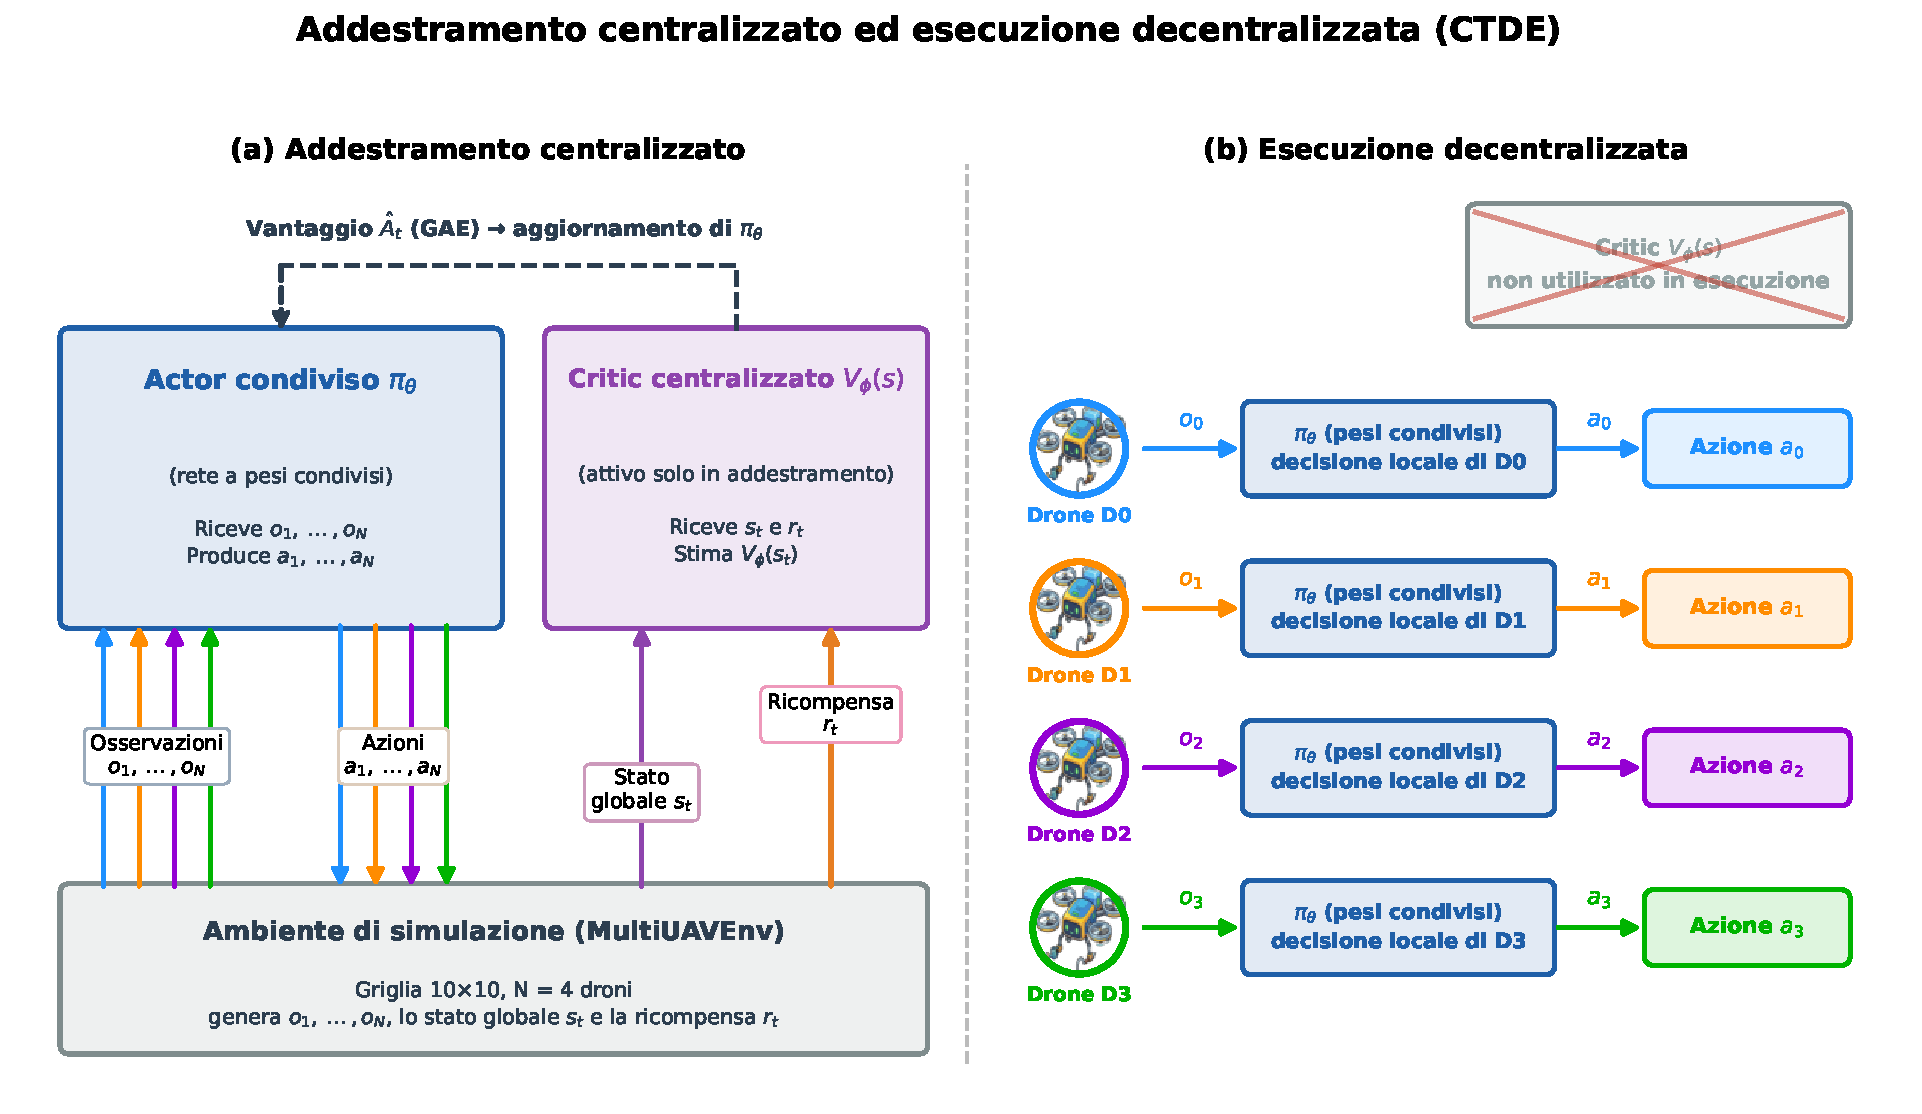
\includegraphics[width=0.95\textwidth]{fig_2_1_ctde.pdf}
    \caption{Addestramento centralizzato ed esecuzione decentralizzata: in addestramento un actor a pesi condivisi riceve le osservazioni locali e un critic centralizzato stima il valore dello stato globale; in esecuzione ciascun drone usa solo il proprio actor.}
    \label{fig:2_1}
\end{figure}

\section{Navigazione multi-agente: Multi-Agent Path Finding, collisioni e stalli}
\label{sec:mapf}

Il problema della navigazione di più agenti verso destinazioni senza collisioni è noto in letteratura come \emph{Multi-Agent Path Finding} (MAPF) \parencite{stern2019}. La formulazione standard modella l'ambiente come un grafo e definisce due classi di conflitto:
\begin{itemize}
    \item il \emph{vertex conflict}, quando due agenti occupano lo stesso nodo nello stesso istante;
    \item l'\emph{edge conflict}, o conflitto di scambio (\emph{swap}), quando due agenti attraversano lo stesso arco in direzioni opposte scambiandosi di posizione.
\end{itemize}

Gli approcci tradizionali al MAPF sono basati su pianificazione, tra cui la pianificazione prioritaria, in cui agli agenti è assegnato un ordine di precedenza e ciascuno pianifica evitando le traiettorie già riservate dagli agenti con priorità maggiore \parencite{silver2005}. Approcci basati su apprendimento, come PRIMAL \parencite{sartoretti2019}, addestrano invece policy decentralizzate che agiscono sulla base di osservazioni locali. Questi ultimi scalano meglio, ma sono esposti a due fenomeni tipici:
\begin{itemize}
    \item il \emph{deadlock} (stallo), in cui due o più agenti restano bloccati in configurazioni dalle quali nessuno riesce a progredire, per esempio ai lati di un passaggio stretto;
    \item il \emph{livelock}, in cui gli agenti si muovono continuamente senza avvicinarsi al proprio obiettivo, per esempio oscillando tra due celle.
\end{itemize}

Le configurazioni più critiche sono quelle in cui una risorsa è unica e condivisa, come nel caso di un solo hangar su cui devono convergere tutti i droni, oppure in cui lo spazio libero è ristretto, come i varchi di una sola cella tra un ostacolo e il bordo della mappa. In queste situazioni l'efficienza individuale delle policy può essere controproducente, poiché porta più agenti a competere nello stesso istante per la stessa cella. Le regole di precedenza utilizzate nella pianificazione prioritaria suggeriscono un possibile rimedio, basato sull'imposizione di un ordine.

% =============================================================================
% CAPITOLO 3 - AMBIENTE DI SIMULAZIONE
% =============================================================================
\chapter{Ambiente di simulazione}
\label{chap:ambiente}

\section{Scelte progettuali}
\label{sec:scelte_progettuali}

Gli esperimenti descritti in questa tesi sono stati condotti in un ambiente di simulazione sviluppato, implementato in Python come estensione della classe base \texttt{gymnasium.Env} \parencite{towers2024}. L'aderenza allo standard Gymnasium garantisce modularità e piena compatibilità con le librerie moderne di reinforcement learning, tra cui Stable-Baselines3 \parencite{raffin2021}, impiegata per la linea di base PPO, e con l'implementazione di MAPPO sviluppata in PyTorch.

Il mondo è modellato come una griglia bidimensionale discreta di dimensione $10 \times 10$, nella quale ogni uav occupa una cella e si sposta di una cella per passo (non diagonalmente). La scelta di un'astrazione discreta, che trascura la dinamica continua del volo, la quota e i vincoli aerodinamici, consente di concentrare l'analisi sul problema del coordinamento tra agenti, mantiene basso il costo computazionale di ciascun passo di simulazione e rende gli esperimenti riproducibili e confrontabili. Il rovescio di questa scelta, è che i risultati non sono direttamente trasferibili a scenari di volo reali.

Sono state realizzate due classi, che riflettono il percorso del lavoro: \texttt{SingleUAVEnv}, ambiente a singolo drone impiegato come prova di fattibilità e linea di base architetturale, e \texttt{MultiUAVEnv}, ambiente parametrico nel numero di droni che costituisce il banco di prova degli esperimenti principali. La seconda mantiene la medesima struttura della prima, estendendola alla gestione di più agenti e delle loro collisioni.

\section{Ambiente a singolo drone}
\label{sec:ambiente_singolo}

L'ambiente \texttt{SingleUAVEnv} rappresenta un singolo UAV che deve raggiungere un bersaglio, detto hangar, su una griglia $10 \times 10$ contenente quattro ostacoli statici (le ``montagne''). A ogni episodio il drone, il bersaglio e gli ostacoli sono collocati in celle distinte, in modo che gli ostacoli non occupino mai la posizione di partenza né quella del bersaglio.

\paragraph{Spazio delle osservazioni.} L'osservazione è un vettore monodimensionale di $12$ interi, $[\text{uav}_x, \text{uav}_y, \text{target}_x, \text{target}_y, \text{ob}_{1,x}, \text{ob}_{1,y}, \dots, \text{ob}_{4,x}, \text{ob}_{4,y}]$, che fornisce all'agente le coordinate del drone, del bersaglio e di ciascun ostacolo.
L'agente dispone quindi di un'informazione completa sulla configurazione del mondo.

\paragraph{Spazio delle azioni.} Lo spazio delle azioni è \texttt{Discrete(5)}, composto da cinque mosse, riportate in Tabella~\ref{tab:3_1}. L'asse verticale è orientato verso il basso, per cui l'azione ``Giù'' incrementa la coordinata $y$.

\begin{table}[htbp]
    \centering
    \begin{tabular}{cll}
        \toprule
        \textbf{Indice} & \textbf{Azione} & \textbf{Spostamento $(\Delta x, \Delta y)$} \\
        \midrule
        0 & Fermo    & $(0, 0)$  \\
        1 & Destra   & $(+1, 0)$ \\
        2 & Giù      & $(0, +1)$ \\
        3 & Sinistra & $(-1, 0)$ \\
        4 & Su       & $(0, -1)$ \\
        \bottomrule
    \end{tabular}
    \caption{Spazio delle azioni individuali, comune a \texttt{SingleUAVEnv} e \texttt{MultiUAVEnv}.}
    \label{tab:3_1}
\end{table}

\paragraph{Funzione di ricompensa e terminazione.} La ricompensa è costruita per insegnare due comportamenti: il raggiungimento rapido dell'obiettivo e l'evitamento degli ostacoli. Essa è composta da:
\begin{itemize}
    \item un premio di $+100$ al raggiungimento dell'hangar, che termina l'episodio con successo (\texttt{terminated = True});
    \item una penalità costante di $-1$ a ogni passo, che incentiva la ricerca del percorso più breve secondo la distanza di Manhattan;
    \item una penalità di $-10$ in caso di tentativo di uscita dai bordi della mappa o di urto contro un ostacolo, accompagnata dall'annullamento del movimento: il drone rimane nella cella precedente.
\end{itemize}
L'episodio è inoltre troncato (\texttt{truncated = True}) dopo $100$ passi.

\paragraph{Visualizzazione.} L'ambiente integra un motore di rendering basato su Pygame (finestra di $768 \times 768$ pixel, in modalità \texttt{render\_mode="human"}), con immagini dedicati per il drone, l'hangar e le montagne. Il rendering è utilizzato solo in fase di verifica visiva dei comportamenti appresi, mentre l'addestramento avviene senza interfaccia grafica per massimizzare il numero di passi al secondo. La Figura~\ref{fig:3_1} mostra una schermata dell'ambiente.

\begin{figure}[htbp]
    \centering
    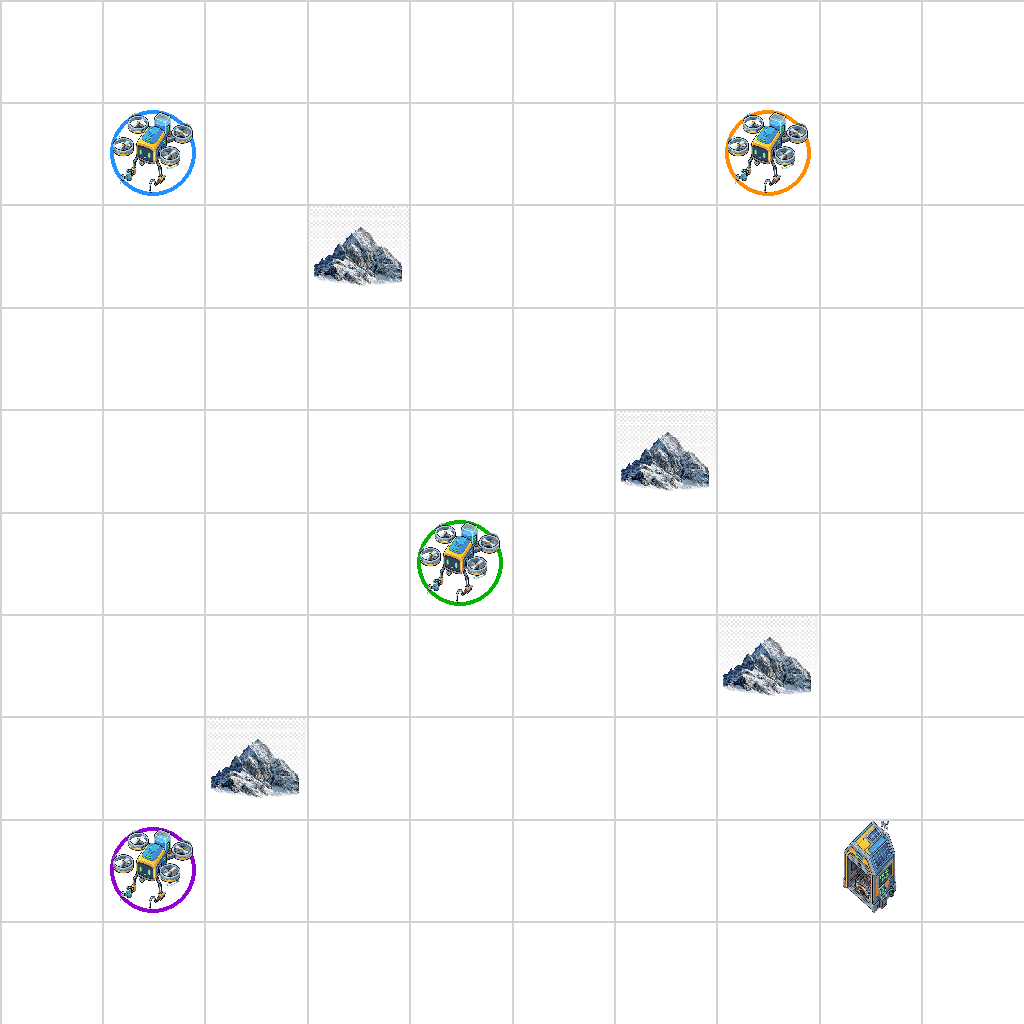
\includegraphics[width=0.65\textwidth]{fig_3_1_simulazione.png}
    \caption{Schermata dell'ambiente di simulazione (Pygame): griglia $10 \times 10$ con quattro droni, identificati dagli anelli cromatici (D0 blu, D1 arancione, D2 viola, D3 verde), quattro ostacoli montuosi e l'hangar in basso a destra.}
    \label{fig:3_1}
\end{figure}

\section{Ambiente multi-agente parametrico}
\label{sec:ambiente_multi}

L'ambiente \texttt{MultiUAVEnv} generalizza il precedente a una flotta di $N$ droni, con $N$ configurabile all'inizializzazione da $1$ a $4$, ad esempio con \texttt{MultiUAVEnv(size=10, num\_obstacles=4, num\_uavs=2)}. Tutti i droni condividono un unico bersaglio comune, l'hangar, e la missione è cooperativa.

\paragraph{Inizializzazione e posizionamento.} Le posizioni dei droni sono mantenute in una lista di coordinate. All'inizio di ogni episodio un insieme di posizioni occupate garantisce che i droni siano collocati in celle distinte tra loro, diverse dall'hangar e dagli ostacoli. In nessun episodio, pertanto, il posizionamento iniziale genera una sovrapposizione.

\paragraph{Spazio delle azioni.} Lo spazio delle azioni è $\texttt{MultiDiscrete}([5] \cdot N)$: a ogni passo l'ambiente riceve un vettore di $N$ interi, uno per drone, scelti tra le cinque azioni di Tabella~\ref{tab:3_1}. Lo spazio delle azioni congiunte ha pertanto cardinalità $5^N$ ($5$, $25$, $125$ e $625$ azioni per $N$ da $1$ a $4$), una crescita esponenziale che costituisce la principale difficoltà per un controllore centralizzato e motiva l'impiego di policy con parametri condivisi.

\paragraph{Spazio delle osservazioni.} Il vettore di stato globale restituito dall'ambiente ha dimensione $2N\text{ (n.\ droni)} + 2 + 2M\text{ (n.\ montagne)}$ e contiene, nell'ordine, le coordinate di tutti i droni, del bersaglio e degli ostacoli:
\[
[\text{uav}_0, \dots, \text{uav}_{N-1}, \text{target}, \text{ob}_1, \dots, \text{ob}_M].
\]
Per $N = 4$ e $M = 4$ si hanno quindi $18$ valori interi (Figura~\ref{fig:3_2}). Per il paradigma CTDE l'ambiente espone inoltre tre metodi di supporto, che preservano la compatibilità con Gymnasium:
\begin{itemize}
    \item \texttt{get\_agent\_obs(i)}, che restituisce l'osservazione ego-centrica del drone $i$: le coordinate proprie, quelle del bersaglio, quelle degli ostacoli e quelle degli altri $N - 1$ droni, in ordine di indice; la dimensione è $2 + 2 + 2M + 2(N - 1) = 2N + 2 + 2M$;
    \item \texttt{get\_all\_agent\_obs()}, che restituisce la matrice $(N, \text{obs\_dim})$ delle osservazioni di tutti i droni;
    \item \texttt{get\_global\_state()}, che fornisce il vettore di stato globale al critic centralizzato, con la stessa composizione di sole coordinate.
\end{itemize}

Tutte le osservazioni contengono esclusivamente coordinate spaziali $(x, y)$. Non è presente alcun indicatore esplicito di arrivo: lo stato di arrivo è usato solo per calcolare il tasso di successo e registrare le metriche, e non entra nelle reti. Quando un drone raggiunge l'hangar, la sua posizione viene fissata alle coordinate del bersaglio, per cui l'atterraggio è deducibile solo dalla coincidenza delle sue coordinate con quelle dell'hangar.

\begin{figure}[htbp]
    \centering
    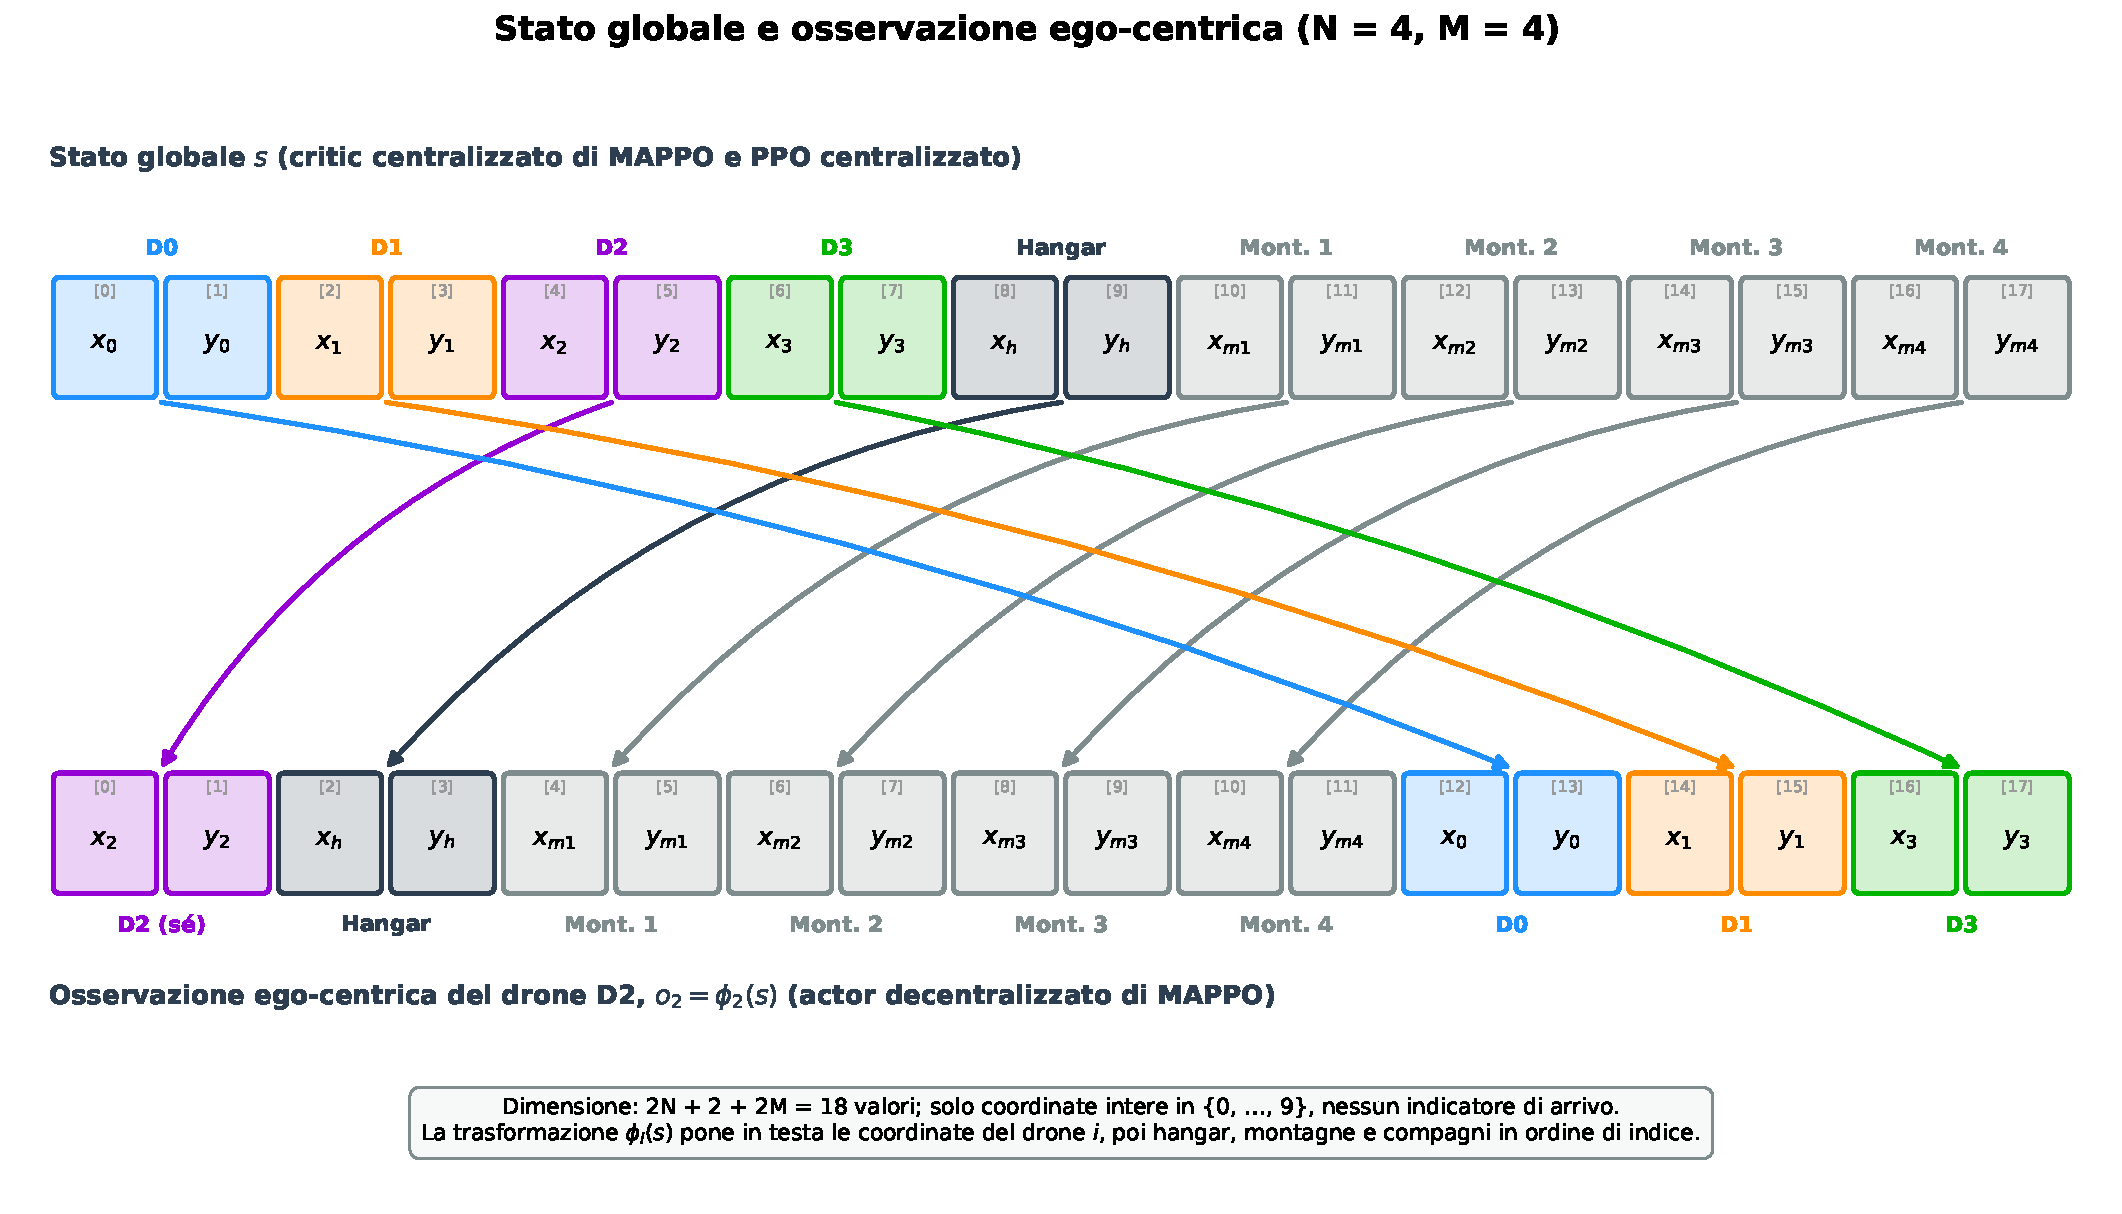
\includegraphics[width=0.95\textwidth]{fig_3_2_osservazione.pdf}
    \caption{Stato globale e osservazione ego-centrica del drone D2 per $N = 4$ e $M = 4$: la trasformazione riordina le stesse $18$ coordinate, ponendo in testa quelle del drone.}
    \label{fig:3_2}
\end{figure}

\paragraph{Confronto tra le due classi.} La Tabella~\ref{tab:3_2} riassume le differenze tra \texttt{SingleUAVEnv} e \texttt{MultiUAVEnv}.

\begin{table}[htbp]
    \centering
    \begin{tabularx}{\textwidth}{l X X}
        \toprule
        \textbf{Caratteristica} & \textbf{SingleUAVEnv} & \textbf{MultiUAVEnv} \\
        \midrule
        Numero di agenti          & 1 (fisso) & da 1 a 4 (parametrico) \\
        Spazio delle azioni       & \texttt{Discrete(5)} & $\texttt{MultiDiscrete}([5] \cdot N)$, $5^N$ combinazioni congiunte \\
        Spazio delle osservazioni & vettore statico di 12 elementi & vettore di $2N + 2 + 2M$ elementi \\
        Obiettivo                 & raggiungimento del bersaglio individuale & arrivo di tutta la flotta all'hangar comune \\
        Collisioni gestite        & bordi e ostacoli & bordi, ostacoli, collisioni tra droni (vertice e scambio) \\
        Ricompensa                & scalare individuale & scalare cooperativo di squadra \\
        \bottomrule
    \end{tabularx}
    \caption{Confronto tra l'ambiente a singolo drone e l'ambiente multi-agente.}
    \label{tab:3_2}
\end{table}

\section{Gestione delle collisioni}
\label{sec:gestione_collisioni}

L'ambiente distingue tre classi di eventi di collisione: l'urto con un ostacolo o con il bordo della mappa, la vertex collision e l'edge collision tra droni.

\paragraph{Urti con ostacoli e bordi.} Quando l'azione di un drone lo porterebbe fuori dalla griglia o in una cella occupata da una montagna, il movimento viene annullato e il drone rimane nella cella precedente. Il drone subisce una penalità individuale di $-10$, come già avviene nell'ambiente a singolo drone.

\paragraph{Vertex collision.} Si ha una vertex collision quando due droni tentano di occupare nello stesso istante la stessa cella, diversa dall'hangar. Indicata con $p_i$ la posizione corrente del drone $i$, con $p_i'$ la posizione che esso assumerebbe a seguito dell'azione scelta e con $h$ la posizione dell'hangar, la condizione è
\[
p_i' = p_j' \neq h, \quad \text{con } i \neq j.
\]
La condizione ricomprende anche il caso in cui uno dei due droni rimanga fermo e l'altro tenti di entrare nella sua cella.

\paragraph{Edge collision (scambio).} Si ha un'edge collision quando due droni adiacenti tentano di scambiarsi di posizione nello stesso passo, ossia quando
\[
p_i' = p_j \quad \text{e} \quad p_j' = p_i.
\]
Senza questo controllo due droni in rotta di collisione frontale si attraverserebbero senza urtarsi, in contraddizione con la natura fisica del problema, perché il test sulla sola cella di destinazione non rileverebbe il conflitto. La Figura~\ref{fig:3_3} illustra le due situazioni.

\begin{figure}[htbp]
    \centering
    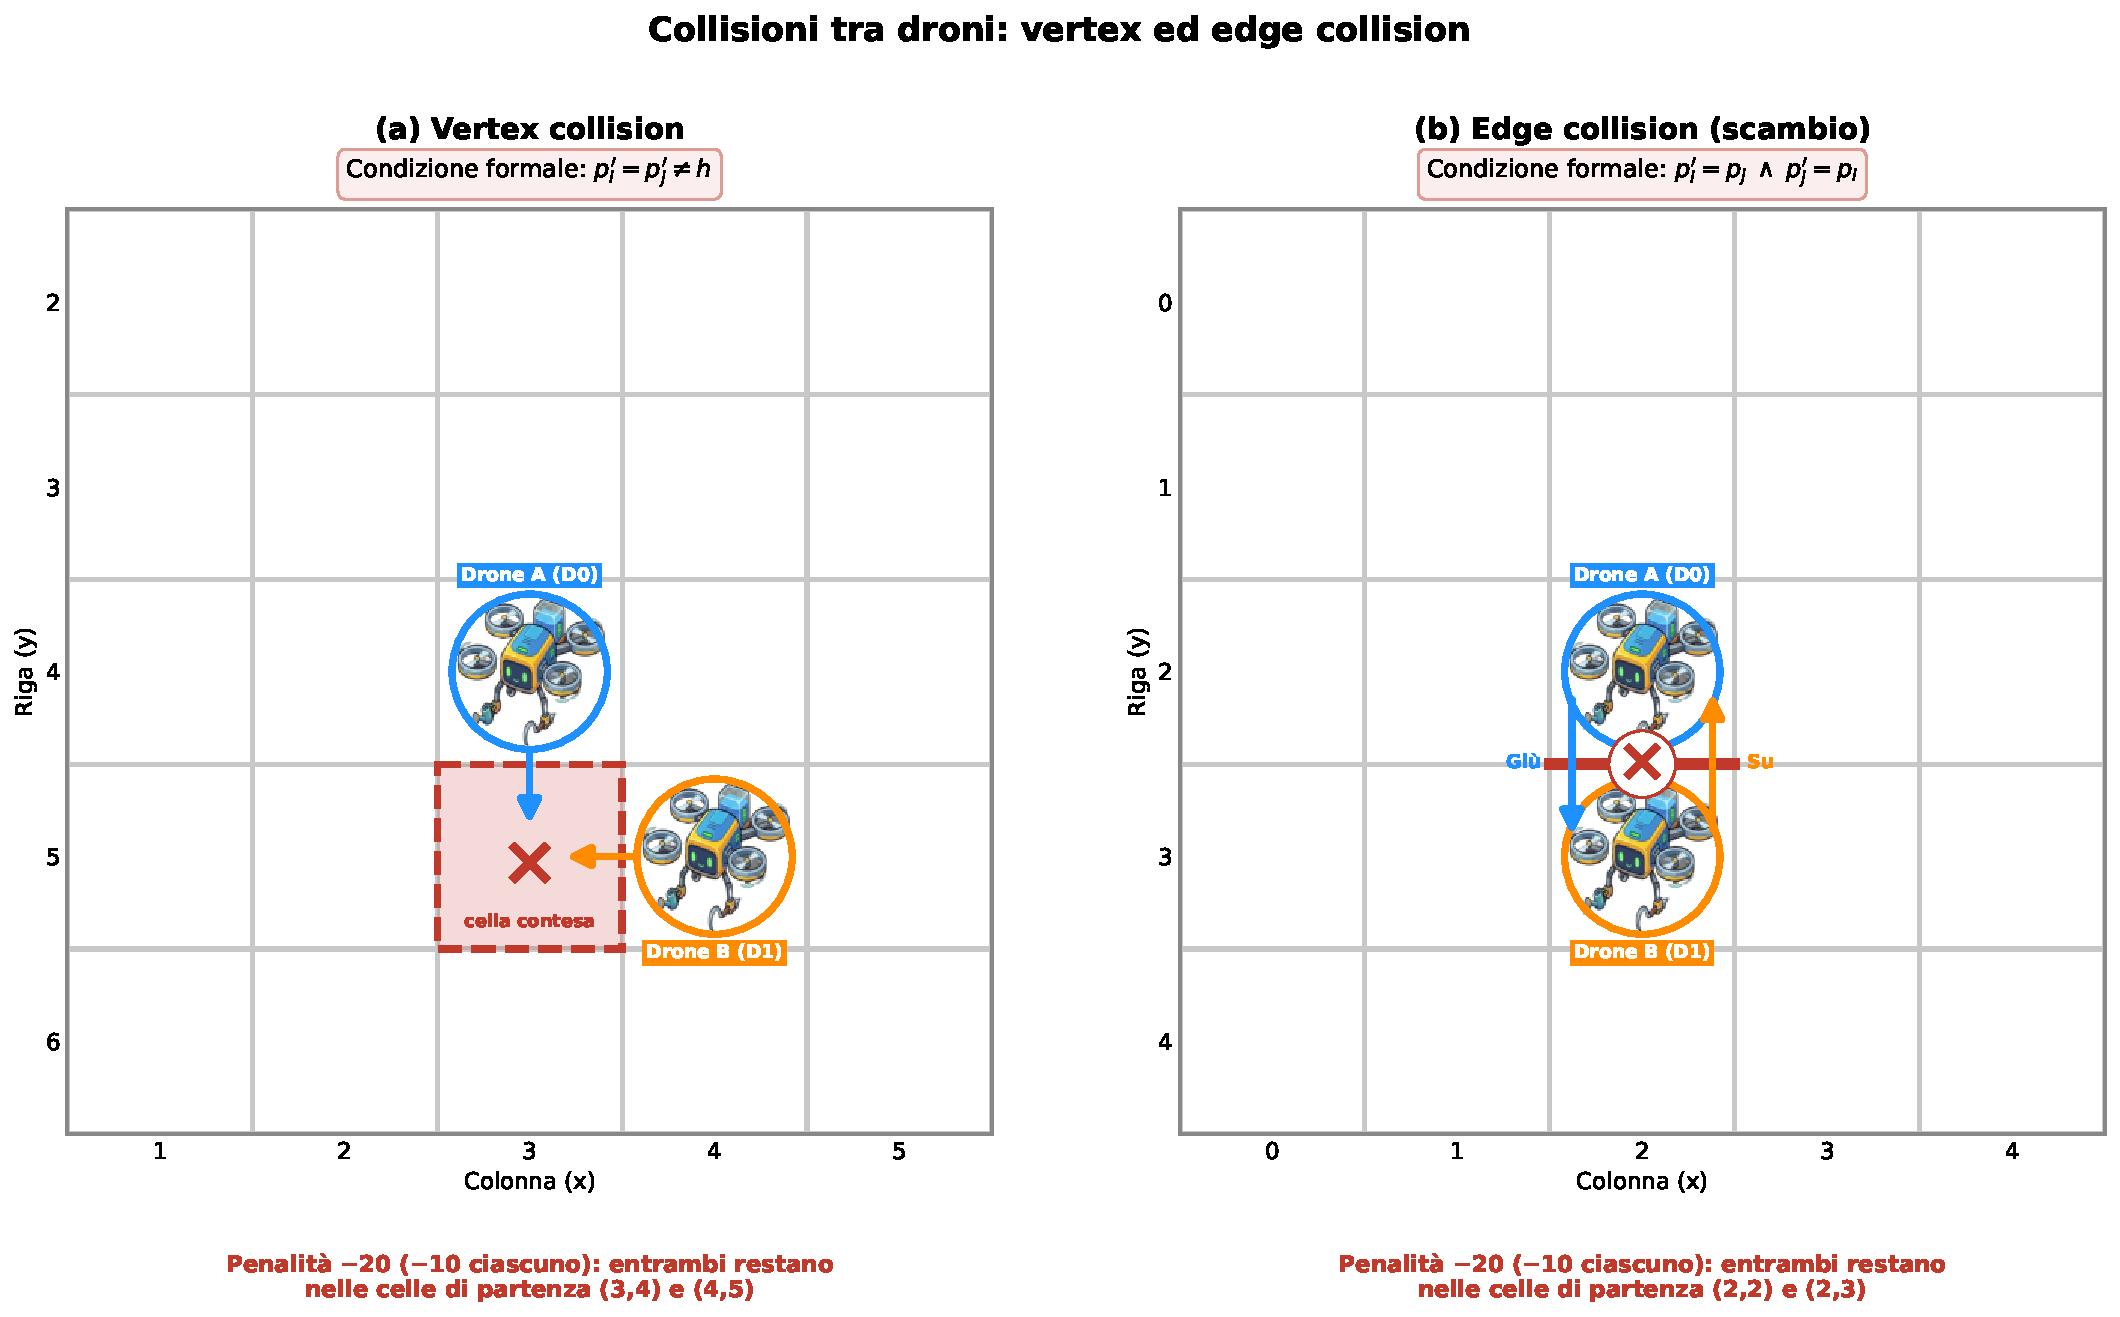
\includegraphics[width=0.95\textwidth]{fig_3_3_collisioni.pdf}
    \caption{Vertex collision (a sinistra) ed edge collision (a destra): esempi con due droni, condizioni formali e relativo blocco del movimento.}
    \label{fig:3_3}
\end{figure}

\paragraph{Ordine di valutazione.} Il metodo \texttt{step()} valuta gli eventi in due stadi sequenziali. Nel primo stadio, per ciascun drone $i$ si calcola la posizione candidata $p_i^{\text{cand}} = p_i + \Delta p_i$: se essa esce dai bordi della mappa o ricade su una montagna, il movimento è annullato (la posizione candidata torna a $p_i$) e si applica la penalità di $-10$. Nel secondo stadio, solo dopo che tutte le posizioni candidate sono state filtrate dal primo, l'ambiente esamina tutte le coppie di droni $(i, j)$ per rilevare le vertex collision sulle posizioni candidate risultanti e le edge collision confrontando le posizioni candidate con quelle correnti. Le condizioni precedenti vanno quindi lette assumendo che $p_i'$ sia la posizione candidata già filtrata dal primo stadio.

L'ordine ha una conseguenza diretta sulle penalità. Se un drone A tenta di entrare in una montagna, il suo movimento è annullato nel primo stadio e A rimane nella cella in cui si trova. Se nello stesso passo un drone B tenta legittimamente di entrare nella cella di A, nel secondo stadio si verifica una vertex collision ($p_B^{\text{cand}} = p_A^{\text{cand}}$). In questo caso A subisce sia la penalità per l'ostacolo ($-10$) sia la propria quota della penalità di collisione ($-10$), mentre B subisce $-10$ e viene respinto nella cella di partenza.

\paragraph{Conseguenze.} Una collisione tra droni, sia vertex sia edge, comporta una penalità congiunta di $-20$, ripartita in $-10$ per ciascuno dei due droni coinvolti nelle ricompense individuali, e il blocco del movimento: entrambi i droni rimangono nelle celle di partenza.

\paragraph{Coabitazione sull'hangar.} L'hangar è l'unica cella in cui più droni possono trovarsi contemporaneamente. Un drone che vi giunge è considerato atterrato e non genera più collisioni con i compagni che sopraggiungono, né nello stesso passo né in passi successivi. Il successo di squadra richiede che tutti gli $N$ droni si trovino contemporaneamente sull'hangar (la condizione di terminazione è \texttt{terminated = all(arrived)}), e un drone atterrato è mantenuto stabilmente sulle coordinate del bersaglio. Se l'hangar fosse soggetto al vincolo di esclusività spaziale, il primo drone atterrato occuperebbe la cella in modo permanente e ogni altro drone che tentasse di atterrare incorrerebbe in una vertex collision, con penalità di $-20$ e respingimento: per $N \ge 2$ la condizione di successo non sarebbe raggiungibile. Per questo la condizione di vertex collision esclude esplicitamente la cella dell'hangar.

\section{Regole del mondo e ricompensa cooperativa}
\label{sec:regole_ricompensa}

Il comportamento dell'ambiente multi-agente è disciplinato da sette regole, implementate nel metodo \texttt{MultiUAVEnv.step()}.
\begin{enumerate}
    \item \textbf{Bersaglio comune.} Sulla mappa è presente un'unica destinazione, l'hangar, condivisa dall'intera flotta.
    \item \textbf{Posizionamento distinto.} All'inizio di ogni episodio tutti i droni sono collocati in celle diverse, senza sovrapporsi tra loro, agli ostacoli o all'hangar.
    \item \textbf{Collisioni tra droni.} Due droni che tentano di entrare nella stessa cella, diversa dall'hangar, oppure di scambiarsi di posizione, subiscono la penalità congiunta di $-20$ ($-10$ ciascuno) e rimangono nelle posizioni di partenza.
    \item \textbf{Atterraggio e coabitazione.} Un drone che raggiunge l'hangar è marcato come arrivato, riceve un premio di $+100$ una tantum e viene mantenuto sulle coordinate del bersaglio. Non paga più la penalità temporale né genera collisioni con i compagni che sopraggiungono.
    \item \textbf{Penalità temporale differenziata.} Ogni drone ancora in volo subisce $-1$ a ogni passo, mentre i droni già atterrati subiscono $0$. Il passo in cui il drone raggiunge l'hangar è compensato dal premio di arrivo e non comporta la penalità temporale. In tal modo la squadra non è penalizzata dall'attesa del completamento della missione da parte dei compagni più lenti.
    \item \textbf{Successo di squadra.} L'episodio termina con successo (\texttt{terminated = all(arrived)}) soltanto quando tutti i droni hanno raggiunto l'hangar. Se questo non accade entro $100$ passi l'episodio è troncato (\texttt{truncated = True}) e considerato fallito.
    \item \textbf{Ricompensa cooperativa.} Il valore restituito a ogni passo è lo scalare complessivo della squadra, che allinea l'interesse di ciascun drone all'efficienza e alla sicurezza collettiva. Le ricompense individuali sono rese disponibili nel dizionario diagnostico \texttt{info} (\texttt{individual\_rewards}), insieme al flag booleano \texttt{success}.
\end{enumerate}

La Tabella~\ref{tab:3_3} riassume gli eventi che concorrono alla ricompensa.

\begin{table}[htbp]
    \centering
    \begin{tabularx}{\textwidth}{l c X}
        \toprule
        \textbf{Evento} & \textbf{Ricompensa} & \textbf{Note} \\
        \midrule
        Arrivo all'hangar                        & $+100$ & una tantum per drone, impedisce l'accumulo nei passi successivi \\
        Passo di volo                            & $-1$   & per ogni drone ancora in volo; $0$ per i droni già atterrati \\
        Urto contro ostacolo o bordo             & $-10$  & individuale; movimento annullato \\
        Collisione tra droni (vertice o spigolo) & $-20$  & congiunta, $-10$ per ciascun drone coinvolto; movimento bloccato \\
        \bottomrule
    \end{tabularx}
    \caption{Eventi dell'ambiente multi-agente e relative ricompense.}
    \label{tab:3_3}
\end{table}

Indicando con $r_{i,t}$ la ricompensa individuale del drone $i$ al passo $t$, il valore restituito dall'ambiente è la ricompensa di squadra $R_t$, somma dei contributi individuali:
\begin{multline*}
R_t = \sum_i r_{i,t}, \quad \text{con } r_{i,t} = +100\text{ (se $i$ atterra al passo $t$)} - 1\text{ (se $i$ è in volo)} \\
- 10\text{ (se $i$ urta un ostacolo o il bordo)} - 10\text{ (se $i$ è coinvolto in una collisione tra droni)}.
\end{multline*}

L'episodio consente di individuare alcuni valori caratteristici della ricompensa cumulativa. Il valore massimo teorico è dato dal solo premio di arrivo, $100 \cdot N$, diminuito del costo temporale dei passi di volo. Il valore di riferimento in assenza di arrivi e di collisioni è invece $N \cdot T_{\max} \cdot (-1) = -N \cdot 100$: per $N = 4$ corrisponde a $-400$. Quest'ultimo non rappresenta un minimo assoluto della ricompensa, poiché le penalità per urti e collisioni possono abbassarla ben oltre tale soglia.

\section{Formalizzazione del modello}
\label{sec:formalizzazione}

Gli elementi del modello sono riassunti nella Tabella~\ref{tab:3_4}.

\begin{table}[htbp]
    \centering
    \begin{tabularx}{\textwidth}{l X}
        \toprule
        \textbf{Elemento} & \textbf{Definizione nell'ambiente} \\
        \midrule
        Agenti $I$         & $N$ droni omogenei, $N \in \{1, \dots, 4\}$; stessa azione, stessa dinamica, stessa ricompensa \\
        Stati $S$          & $s = (p_1, \dots, p_N, h, b_1, \dots, b_M)$, con posizioni in $\{0, \dots, L - 1\}^2$, $L = 10$; hangar $h$ e ostacoli $b_k$ fissi durante l'episodio \\
        Azioni $A_i$       & $\{\text{Fermo}, \text{Destra}, \text{Giù}, \text{Sinistra}, \text{Su}\}$; azione congiunta in $A^N$, di cardinalità $5^N$ \\
        Transizione $P$    & deterministica data l'azione congiunta, secondo le regole delle Sezioni~\ref{sec:gestione_collisioni} e \ref{sec:regole_ricompensa} \\
        Stato iniziale     & estratto a caso a ogni episodio (posizioni distinte), con seme fissato per la riproducibilità \\
        Ricompensa $r$     & ricompensa di squadra $R_t$ della Sezione~\ref{sec:regole_ricompensa} \\
        Orizzonte          & $T_{\max} = 100$ passi; terminazione quando tutti i droni sono atterrati \\
        Osservazione $o_i$ & $o_i = \varphi_i(s)$: riorganizzazione ego-centrica dello stato \\
        \bottomrule
    \end{tabularx}
    \caption{Elementi del modello dell'ambiente.}
    \label{tab:3_4}
\end{table}

\paragraph{Funzione di osservazione.} L'osservazione del drone $i$ è ottenuta dallo stato globale mediante la trasformazione $s \to o_i$, che dispone nell'ordine le coordinate del drone $i$, quelle del bersaglio, quelle degli ostacoli e quelle degli altri $N - 1$ droni in ordine di indice. Tale trasformazione non nasconde alcuna porzione della mappa: l'osservazione contiene la stessa informazione dello stato globale, a meno dell'etichettatura degli agenti, per cui ciascun drone conosce sempre le posizioni di tutti gli altri, del bersaglio e degli ostacoli. Disponendo le informazioni proprie sempre nelle stesse posizioni del vettore, essa rende l'osservazione ego-centrica, così che un'unica rete con parametri condivisi possa governare tutti i droni omogenei (parameter sharing) senza dover distinguere gli agenti tramite l'indice.

\paragraph{Implicazioni.} Poiché l'osservabilità è completa, l'incertezza di ciascun agente non riguarda lo stato del mondo, ma le azioni che i compagni sceglieranno nello stesso istante, e l'esecuzione decentralizzata esclude qualsiasi comunicazione tra i droni. Il problema è pertanto di coordinamento. Il vantaggio del critic centralizzato, che riceve lo stato globale, non consiste quindi in un'informazione ulteriore sullo stato, ma nella stima del valore dello stato congiunto durante l'addestramento.

% =============================================================================
% CAPITOLO 4 - METODI: PPO E MAPPO
% =============================================================================
\chapter{Metodi: PPO e MAPPO}
\label{chap:metodi}

Il capitolo descrive i due approcci di apprendimento confrontati nella tesi: MAPPO, algoritmo esistente di cui è stata realizzata un'implementazione propria in PyTorch, e una linea di base PPO centralizzata, ottenuta con la libreria Stable-Baselines3.

\section{MAPPO con parameter sharing}
\label{sec:mappo}

L'algoritmo MAPPO (\emph{Multi-Agent Proximal Policy Optimization}) \parencite{yu2022} è un algoritmo esistente, di cui è stata realizzata un'implementazione propria in PyTorch (modulo \texttt{src/mappo.py}) secondo il paradigma CTDE, con condivisione dei parametri tra i droni omogenei della flotta. L'implementazione è parametrica nel numero di droni e si appoggia ai metodi dell'ambiente descritti nella Sezione~\ref{sec:ambiente_multi} (\texttt{get\_agent\_obs}, \texttt{get\_all\_agent\_obs}, \texttt{get\_global\_state}); un metodo di supporto, \texttt{extract\_agent\_observations()}, ricostruisce le osservazioni locali a partire dal vettore globale mantenendo il layout ego-centrico di sole coordinate.

L'implementazione riprende gli elementi essenziali dell'algoritmo: actor con parametri condivisi, critic centralizzato sullo stato globale, stima dell'advantage con GAE e clipped objective con value clipping. Non include la normalizzazione della value function in quanto, con una griglia così piccola e un orizzonte di al più $100$ passi, i rendimenti ricadono in un intervallo limitato e noto a priori.

\paragraph{Actor decentralizzato.} Ogni drone $i$ riceve la propria osservazione locale $o_i$, in formato ego-centrico: coordinate proprie, coordinate del bersaglio, coordinate degli ostacoli e posizioni degli altri $N - 1$ droni.

Per il parameter sharing i pesi dell'actor sono condivisi tra tutti i droni. La dimensione dell'uscita rimane quindi fissa a $5$ al crescere di $N$, e la rete apprende contemporaneamente dall'esperienza di tutti i velivoli. Per $N = 1$ l'osservazione locale coincide con lo stato globale e MAPPO si riduce al PPO a singolo agente; per $N > 1$ la stessa architettura gestisce in modo omogeneo flotte di $2$, $3$ e $4$ droni, senza modifiche alla struttura interna.

\paragraph{Critic centralizzato.} Durante l'addestramento il critic stima la value function $V(s)$ a partire dallo stato globale $s$, che comprende le coordinate di tutti i droni, del bersaglio e degli ostacoli.

Il critic non viene utilizzato in fase di esecuzione, in accordo con il paradigma CTDE: ciascun drone, durante il volo, dispone del solo actor.

\paragraph{stima dell'advantage.} I rendimenti e gli advantage sono calcolati con la Generalized Advantage Estimation.

\paragraph{Obiettivo di ottimizzazione.} L'actor massimizza il clipped objective di PPO con un termine di entropia:
\[
L_{\text{actor}}(\theta) = \mathbb{E}_t \left[ \min\left( \rho_t(\theta) \cdot \hat{A}_t , \operatorname{clip}(\rho_t(\theta), 1 - \varepsilon, 1 + \varepsilon) \cdot \hat{A}_t \right) \right] + c_H \cdot H[\pi_\theta],
\]
con $\varepsilon = 0,2$ e coefficiente di entropia $c_H = 0,01$, mentre il critic è addestrato con una funzione di perdita con value clipping. Per ciascun lotto di esperienza si eseguono $10$ epoche di ottimizzazione su minibatch di $64$ campioni, con limitazione della norma del gradiente a $0,5$. I valori degli iperparametri sono riportati in Tabella~\ref{tab:4_1}.

\paragraph{Ottimizzazione e dimensione dei lotti.} Actor e critic sono ottimizzati con due istanze separate dell'ottimizzatore Adam ($\varepsilon = 10^{-5}$), con learning rate rispettivamente di $3 \cdot 10^{-4}$ e $1 \cdot 10^{-3}$. Il valore più elevato per il critic è una prassi consolidata in MAPPO: accelera la convergenza della stima di $V(s)$ e fornisce all'actor advantage più stabili fin dalle prime fasi. Il parametro \texttt{n\_steps} conta i passi congiunti di interazione con l'ambiente (una chiamata a \texttt{env.step()}), non i campioni per agente. L'advantage $\hat{A}_t$ è calcolato dalla ricompensa di squadra e da $V(s_t)$, ed è quindi comune a tutti i droni nello stesso passo. In fase di aggiornamento, grazie al parameter sharing, le transizioni sono srotolate per agente: il critic riceve $1024$ campioni di stato globale per aggiornamento, indipendentemente da $N$, mentre l'actor, che elabora le tuple $(o_i^t, a_i^t, \hat{A}_t)$ di tutti i droni, è ottimizzato su $1024 \cdot N$ campioni ($1024$, $2048$, $3072$ e $4096$ per $N$ da $1$ a $4$).

\begin{table}[htbp]
    \centering
    \begin{tabular}{lc}
        \toprule
        \textbf{Iperparametro} & \textbf{Valore} \\
        \midrule
        Learning rate actor                    & $3 \cdot 10^{-4}$ \\
        Learning rate critic                   & $1 \cdot 10^{-3}$ \\
        Fattore di sconto $\gamma$             & $0,99$ \\
        Parametro GAE $\lambda$                & $0,95$ \\
        Parametro di clipping $\varepsilon$    & $0,2$  \\
        Coefficiente di entropia               & $0,01$ \\
        Passi per aggiornamento (\texttt{n\_steps}) & $1024$ \\
        Dimensione del minibatch               & $64$   \\
        Epoche di ottimizzazione per lotto     & $10$   \\
        Norma massima del gradiente            & $0,5$  \\
        \bottomrule
    \end{tabular}
    \caption{Iperparametri di MAPPO utilizzati in tutti gli esperimenti.}
    \label{tab:4_1}
\end{table}

\begin{figure}[htbp]
    \centering
    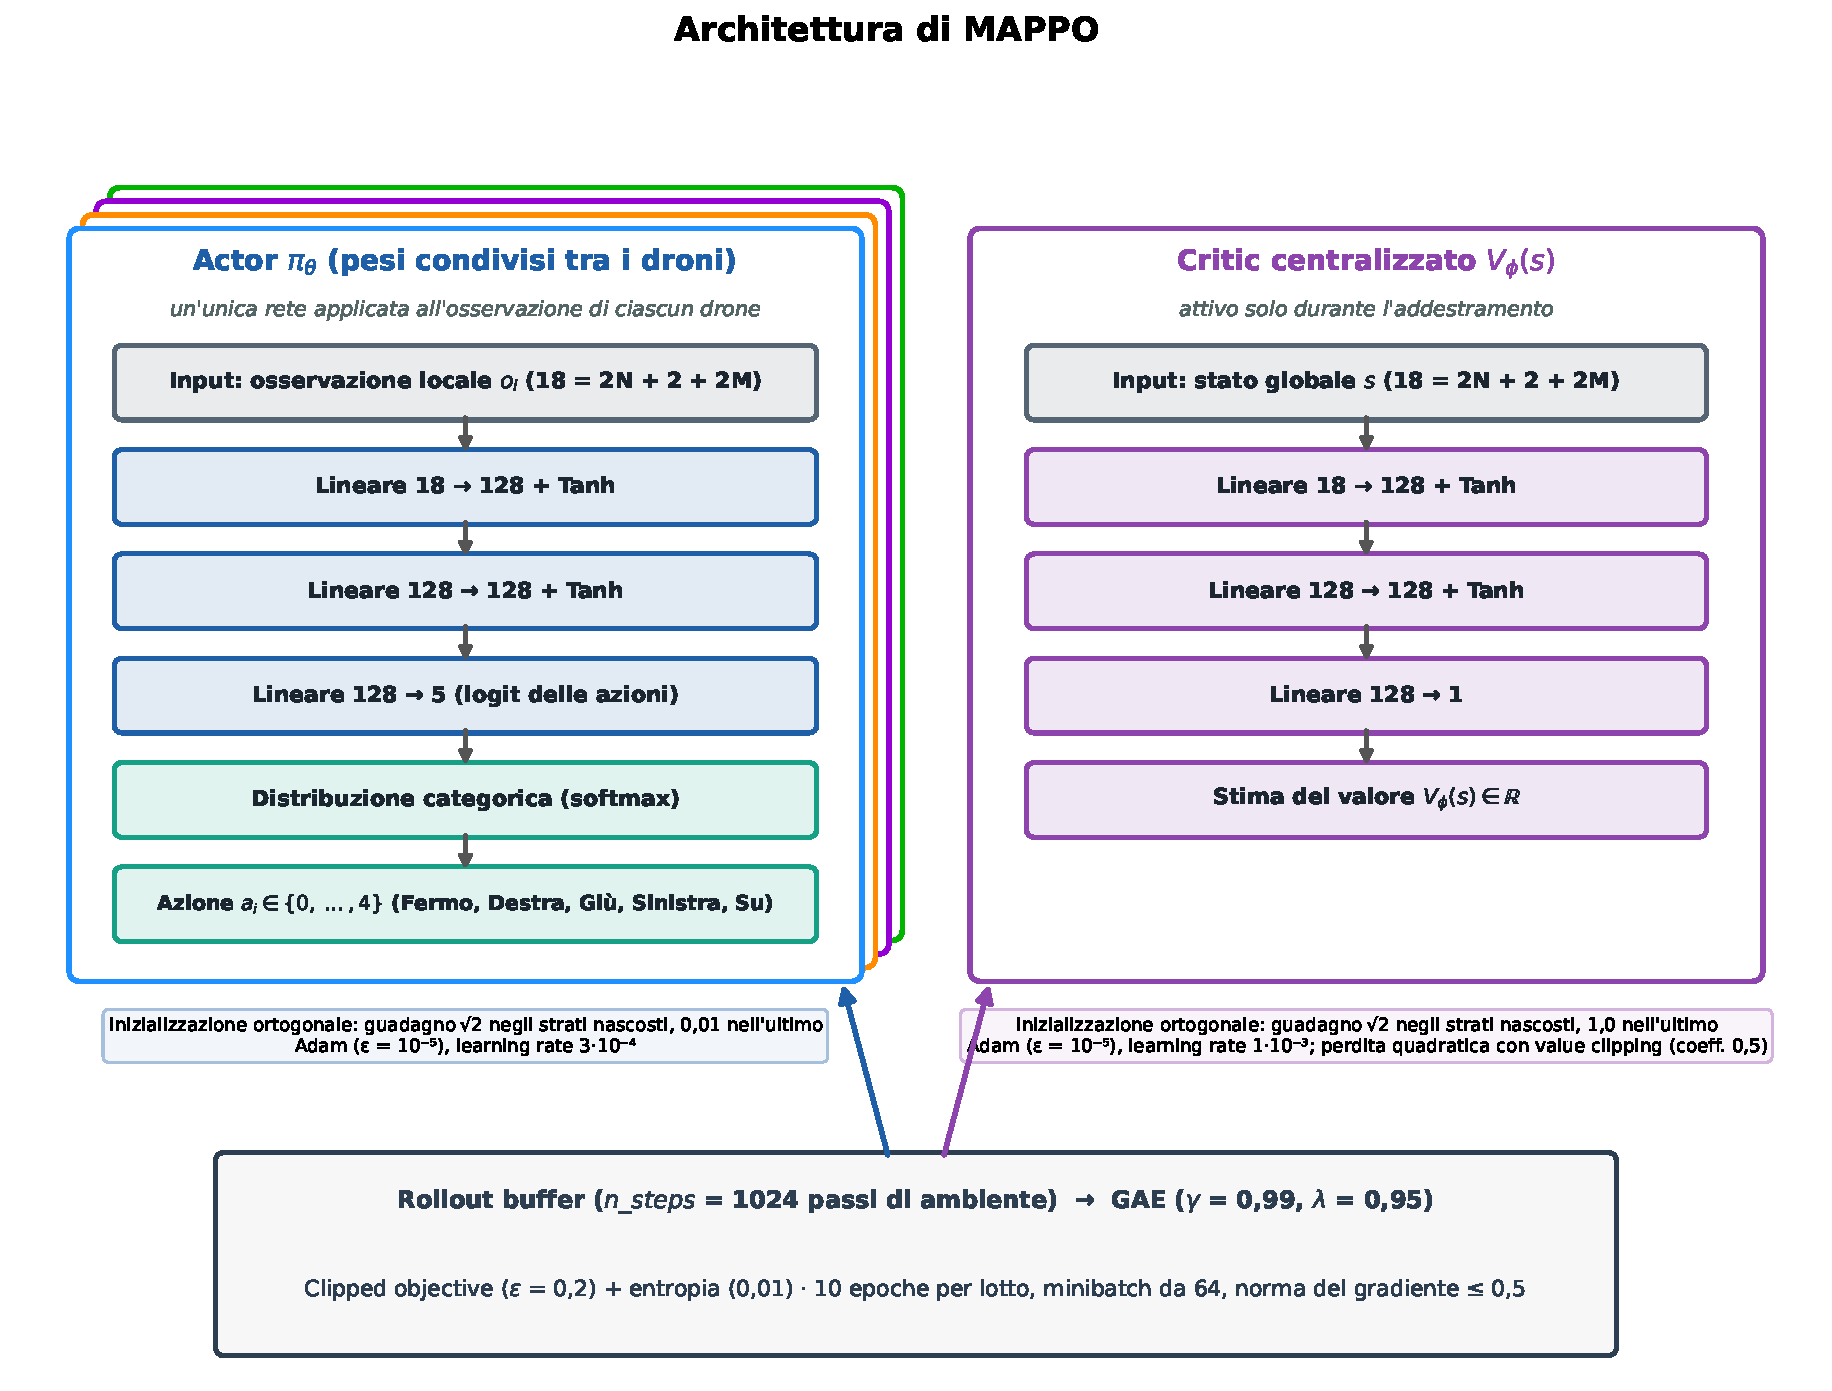
\includegraphics[width=0.95\textwidth]{fig_4_1_architettura_mappo.pdf}
    \caption{Architettura di MAPPO: actor a pesi condivisi applicato all'osservazione locale di ciascun drone e critic centralizzato sullo stato globale, con il ciclo di aggiornamento (buffer, GAE, clipped objective).}
    \label{fig:4_1}
\end{figure}

\section{PPO centralizzato (linea di base)}
\label{sec:ppo_baseline}

Come linea di base si impiega l'algoritmo PPO nell'implementazione di Stable-Baselines3, con policy \texttt{MlpPolicy}, adatta all'elaborazione di vettori numerici monodimensionali come le coordinate. Tutti gli iperparametri sono quelli predefiniti della libreria, utilizzati senza alcuna modifica (Tabella~\ref{tab:4_2}).

L'algoritmo è applicato direttamente all'ambiente \texttt{MultiUAVEnv}, senza alcun adattatore, e quindi allo spazio di azioni nativo $\texttt{MultiDiscrete}([5] \cdot N)$. L'osservazione fornita alla rete è il vettore globale canonico di $2N + 2 + 2M$ coordinate assolute intere, non scalate:
\[
s = [x_0, y_0, \dots, x_{N-1}, y_{N-1}, x_{\text{target}}, y_{\text{target}}, x_{\text{obs},1}, y_{\text{obs},1}, \dots, x_{\text{obs},M}, y_{\text{obs},M}].
\]
Le coordinate dei droni compaiono nell'ordine fisso dell'indice, senza alcun riordinamento ego-centrico: le posizioni $[0, 1]$ appartengono sempre al drone $0$, le posizioni $[2, 3]$ al drone $1$, e così via.

Per gli spazi \texttt{MultiDiscrete} Stable-Baselines3 impiega una distribuzione multicategorica. Lo strato di uscita della rete non produce $5^N$ valori, ma $5 \cdot N$ logit ($20$ per $N = 4$).
Il numero di pesi dello strato finale cresce dunque linearmente con $N$, ma lo spazio congiunto delle configurazioni d'azione da esplorare resta combinatorio ($5^N$). La rete deve apprendere il coordinamento delle $N$ uscite simultanee a partire da un unico vettore di stato. Poiché le uscite dei diversi droni sono distinte e l'osservazione non è ego-centrica, non esiste alcuna condivisione di parametri tra i droni: ciò che la rete apprende per un drone non è riutilizzabile per gli altri, dato che i loro ingressi e le loro uscite occupano posizioni diverse del tensore. Al tempo stesso, la distinzione tra le uscite consente alla policy deterministica di assegnare comportamenti diversi a droni in configurazioni equivalenti, cosa che non è possibile con un actor condiviso a osservazioni ego-centriche.

Il controllo è inoltre centralizzato anche in esecuzione: l'unica rete richiede lo stato globale di tutta la flotta e comanda tutti i droni, il che presuppone un nodo centrale connesso con latenza trascurabile ai velivoli. Si tratta di un vincolo che MAPPO non ha.

\begin{table}[htbp]
    \centering
    \begin{tabularx}{\textwidth}{l X}
        \toprule
        \textbf{Iperparametro} & \textbf{Valore} \\
        \midrule
        Policy                                      & \texttt{MlpPolicy} (reti separate per policy e valore, 2 strati da 64 unità, attivazione Tanh) \\
        Learning rate                               & $3 \cdot 10^{-4}$ \\
        Passi per aggiornamento (\texttt{n\_steps}) & $2048$ \\
        Dimensione del minibatch                    & $64$   \\
        Epoche di ottimizzazione per lotto          & $10$   \\
        Fattore di sconto $\gamma$                  & $0,99$ \\
        Parametro GAE $\lambda$                     & $0,95$ \\
        Parametro di clipping $\varepsilon$         & $0,2$  \\
        Coefficiente di entropia                    & $0,0$  \\
        Coefficiente della value function           & $0,5$  \\
        Norma massima del gradiente                 & $0,5$  \\
        Normalizzazione degli advantage             & attiva \\
        \bottomrule
    \end{tabularx}
    \caption{Iperparametri della linea di base PPO (valori predefiniti di Stable-Baselines3 v2.9.0).}
    \label{tab:4_2}
\end{table}

Poiché il rollout buffer ha dimensione $\texttt{n\_steps} = 2048$, il numero di passi effettivamente eseguiti da Stable-Baselines3 è il primo multiplo di $2048$ non inferiore al budget richiesto (ad esempio $51.200$ passi per un budget di $50.000$ e $501.760$ per $500.000$).

\section{Confronto tra le due configurazioni}
\label{sec:confronto_configurazioni}

La Tabella~\ref{tab:4_3} riassume le differenze tra le due configurazioni.

\begin{table}[htbp]
    \centering
    \begin{tabularx}{\textwidth}{l X X}
        \toprule
        \textbf{Aspetto} & \textbf{PPO centralizzato} & \textbf{MAPPO} \\
        \midrule
        Osservazione                       & vettore globale assoluto, ordine fisso dei droni & osservazione locale ego-centrica \\
        Policy                             & fattorizzata, $5 \cdot N$ logit, un'unica rete per tutti i droni & actor condiviso, $5$ logit per drone \\
        Parameter sharing                  & no & sì \\
        Esecuzione                         & centralizzata (stato globale e controllore unico) & decentralizzata (solo osservazione propria) \\
        Passi di ambiente per aggiornamento & $2048$ & $1024$ \\
        Campioni dell'actor per aggiornamento & $2048$, indipendenti da $N$ & $1024 \cdot N$ \\
        Learning rate                      & $3 \cdot 10^{-4}$ & $3 \cdot 10^{-4}$ (actor), $1 \cdot 10^{-3}$ (critic) \\
        Coefficiente di entropia           & $0,0$ & $0,01$ \\
        \bottomrule
    \end{tabularx}
    \caption{Confronto tra la linea di base PPO centralizzata e MAPPO.}
    \label{tab:4_3}
\end{table}

Le due configurazioni differiscono quindi non solo per l'approccio di apprendimento (condivisione dei parametri, osservazione ego-centrica, esecuzione decentralizzata), ma anche per diversi iperparametri. Il bonus di entropia in MAPPO contrasta la convergenza prematura verso una policy quasi deterministica, mentre PPO ne è privo. Le differenze di prestazione osservate non possono pertanto essere attribuite al solo paradigma CTDE o al parameter sharing.

Per $N = 1$ le due configurazioni coincidono nella struttura del problema (osservazione locale e globale identiche) e differiscono solo per l'implementazione e per gli iperparametri.

% =============================================================================
% CAPITOLO 5 - SETUP SPERIMENTALE
% =============================================================================
\chapter{Setup sperimentale}
\label{chap:setup}

Il capitolo descrive il protocollo con cui sono stati addestrati e valutati MAPPO e PPO centralizzato: configurazioni sperimentali, budget di addestramento, gestione dei semi, procedura di valutazione, metriche e piattaforma di calcolo.

\section{Configurazioni sperimentali}
\label{sec:configurazioni_sperimentali}

Le configurazioni sono definite dal numero di droni $N$ e dall'algoritmo. Il codice dell'ambiente è parametrico fino a $4$ droni; per la tesi si è scelto di iniziare da un drone, validare con tre e spingere l'analisi dei casi limite fino a quattro. Le motivazioni sono tre. Anzitutto, lo spazio delle azioni congiunte cresce come $5^N$ ($5$, $25$, $125$ e $625$ combinazioni per $N$ da $1$ a $4$), il che richiede un numero crescente di passi di addestramento per esplorare e convergere. In secondo luogo, da due a quattro droni l'addestramento converge in tempi ragionevoli su un pc dotato di GPU dedicata (NVIDIA RTX 4060), senza ricorrere a un cluster. Infine, la parametricità permette un confronto completo da $N = 1$ a $N = 4$, utile per quantificare come cresce la difficoltà di coordinamento con la flotta.

La Tabella~\ref{tab:5_1} riassume le configurazioni. Il confronto principale riguarda $N$ da $1$ a $4$ con budget differenziati, a cui si aggiunge uno studio asintotico a quattro droni con $4.000.000$ di passi.

\begin{table}[htbp]
    \centering
    \resizebox{\textwidth}{!}{%
    \begin{tabular}{lccccc}
        \toprule
        \textbf{Esperimento} & \textbf{Droni $N$} & \textbf{Algoritmi} & \textbf{Budget di addestramento (passi)} & \textbf{Semi} & \textbf{Valutazione} \\
        \midrule
        Confronto 1--4 droni & 1 & MAPPO, PPO & $150.000$   & 42, 123, 999 & 100 episodi per seme \\
                             & 2 & MAPPO, PPO & $450.000$   & 42, 123, 999 & 100 episodi per seme \\
                             & 3 & MAPPO, PPO & $750.000$   & 42, 123, 999 & 100 episodi per seme \\
                             & 4 & MAPPO, PPO & $1.000.000$ & 42, 123, 999 & 100 episodi per seme \\
        \midrule
        Studio singolo       & 4 & MAPPO, PPO & $4.000.000$ & 42, 123, 999 & 100 episodi per seme \\
        \bottomrule
    \end{tabular}%
    }
    \caption{Configurazioni sperimentali.}
    \label{tab:5_1}
\end{table}

A queste si aggiungono l'analisi della scomposizione della ricompensa a quattro droni e il test dello strato di risoluzione dei conflitti, che comprende cinque scenari critici posizionati manualmente e una valutazione statistica su $300$ episodi.

Le curve di addestramento registrate con TensorBoard sono disponibili per MAPPO da uno a quattro droni e per PPO a uno e due droni, nelle run di calibrazione descritte nel Capitolo~\ref{chap:risultati_1}, e per entrambi gli algoritmi nello studio a $4.000.000$ di passi.

\section{Budget di addestramento}
\label{sec:budget_addestramento}

Nel reinforcement learning la prestazione non migliora indefinitamente con il numero di passi. Un addestramento segue tipicamente tre fasi: una fase di crescita rapida (\emph{under-training}), in cui la policy passa da comportamenti con collisioni continue alla comprensione delle regole di base; un plateau di convergenza, in cui aggiungere passi produce solo guadagni marginali; e una fase di instabilità o sovra-addestramento (\emph{over-training}), in cui aggiornamenti bruschi o un eccessivo sfruttamento possono degradare la policy, ad esempio rendendola eccessivamente deterministica. Il criterio operativo adottato è l'osservazione delle curve di apprendimento: se al termine dell'addestramento la curva del reward è ancora in forte salita, il training è stato interrotto prematuramente; se è già piatta da $200.000$--$300.000$ passi, la policy ha raggiunto il massimo consentito dall'architettura e dalle regole di esecuzione.

\begin{figure}[htbp]
    \centering
    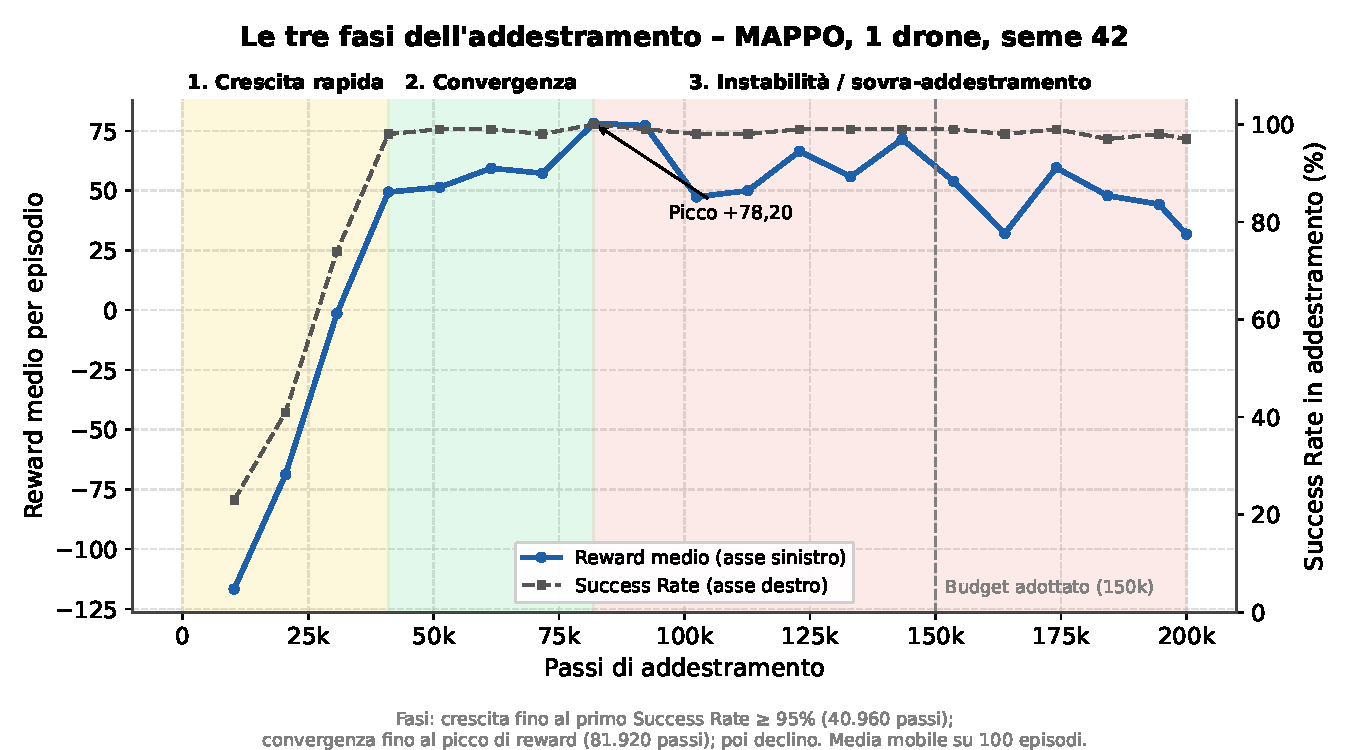
\includegraphics[width=0.95\textwidth]{fig_5_1_tre_fasi_training.pdf}
    \caption{Le tre fasi dell'addestramento su una curva reale: reward medio e Success Rate in addestramento di MAPPO a un drone, seme $42$. Crescita rapida fino al primo $\text{Success Rate} \ge 95\%$ ($40.960$ passi), convergenza fino al picco di reward ($+78,20$ a $81.920$ passi), poi declino fino a $+31,77$ a $200.000$ passi.}
    \label{fig:5_1}
\end{figure}

I budget del confronto principale ($150.000$, $450.000$, $750.000$ e $1.000.000$ di passi) sono stati calibrati sulla complessità combinatoria della flotta, a partire da run esplorative con $200.000$ passi per un drone, $500.000$ per due, $750.000$ per tre e $1.000.000$ per quattro. Lo studio a quattro droni con $4.000.000$ di passi verifica se il basso tasso di successo osservato possa essere risolto aumentando il budget.

Il PPO di Stable-Baselines3 esegue un numero di passi pari al primo multiplo di \texttt{n\_steps} ($2048$) non inferiore al budget richiesto: $50.000$ passi diventano $51.200$, $200.000$ diventano $200.704$, $500.000$ diventano $501.760$ e $4.000.000$ diventano $4.001.792$; i budget del confronto principale ($150.000$, $450.000$, $750.000$ e $1.000.000$) diventano rispettivamente $151.552$, $450.560$, $751.616$ e $1.001.472$. L'implementazione di MAPPO verifica invece il budget a ogni singolo passo di interazione e si arresta esattamente al valore nominale. Gli scarti per PPO restano inferiori all'$1\%$ e sono trascurabili ai fini del confronto.

\section{Riproducibilità e gestione dei semi}
\label{sec:riproducibilita}

Per garantire riproducibilità sui risultati viene introdotto il seme del generatore pseudo-casuale che controlla l'inizializzazione dei pesi, il campionamento delle azioni e la generazione procedurale di posizioni di partenza, hangar e ostacoli. Rieseguendo con lo stesso seme, produce le stesse curve di reward e le stesse metriche. Ne derivano tre vantaggi metodologici:
\begin{itemize}
    \item \textbf{Riproducibilità.} Un esperimento rieseguito a distanza di tempo da altri produce gli stessi risultati.
    \item \textbf{Confronti equi.} Nel confronto tra algoritmi (MAPPO e PPO) o tra configurazioni ($N$ droni), lo stesso seme garantisce la stessa sequenza di mappe generate, per cui le differenze di prestazione sono attribuibili all'algoritmo e non alla fortuna degli spawn.
    \item \textbf{Debugging deterministico.} Un comportamento anomalo osservato in un episodio (una collisione complessa, un vicolo cieco) può essere rieseguito identico per analizzarlo nel dettaglio.
\end{itemize}

Fissare il seme non significa che la mappa sia sempre la stessa: il generatore produce una sequenza deterministica di episodi, ciascuno con una configurazione diversa, per cui la flotta continua ad apprendere su mappe sempre nuove, ma la sequenza complessiva è identica da un'esecuzione all'altra. Nella prima fase del lavoro è stato usato solo il seme $42$. Il benchmark conclusivo utilizza tre semi indipendenti ($42$, $123$ e $999$): ciascuno produce un modello distinto, addestrato e valutato separatamente, e i risultati sono aggregati come media e deviazione standard campionaria sui tre semi.

\section{Protocollo di valutazione}
\label{sec:protocollo_valutazione}

Le policy addestrate sono valutate su $100$ episodi per seme, per un totale di $300$ episodi per configurazione. Gli episodi di valutazione sono generati con lo stesso seme dell'addestramento, ma costituiscono una sequenza di mappe nuova, non osservata durante l'addestramento. Tutte le valutazioni sono deterministiche: l'azione eseguita è quella a massima probabilità (\texttt{deterministic=True} per PPO, selezione per massimo logit per MAPPO), senza campionamento. Questa scelta differenzia le metriche di valutazione da quelle di addestramento, che derivano da policy stocastiche.

La scelta del numero di episodi è motivata dalla varianza campionaria. La prima versione del protocollo utilizzava $10$ episodi per configurazione. Per un tasso di successo $p$ stimato su $n$ episodi, l'errore standard della stima è $\sqrt{p(1 - p)/n}$, che nel caso peggiore ($p = 0,5$) vale circa $\pm 15\%$ per $n = 10$, $\pm 5\%$ per $n = 100$ e $\pm 3\%$ per i $300$ episodi complessivi. Con soli $10$ episodi un singolo episodio sposta la metrica del $10\%$, e uno spawn favorevole o sfavorevole può distorcere il risultato.

Il costo computazionale della valutazione è trascurabile rispetto all'addestramento. La valutazione è pura inferenza in avanti (\texttt{torch.no\_grad()}), senza calcolo di gradienti né ottimizzazione e senza rendering grafico: con un throughput superiore a $4.000$ passi al secondo e circa $50$ passi per episodio, $100$ episodi richiedono circa $1,3$ secondi e l'intera suite di otto valutazioni circa $11$ secondi, cioè lo $0,24\%$ del tempo totale.

\section{Metriche}
\label{sec:metriche}

Le metriche sono riportate nella Tabella~\ref{tab:5_2}.

\begin{table}[htbp]
    \centering
    \begin{tabularx}{\textwidth}{l X}
        \toprule
        \textbf{Metrica} & \textbf{Definizione} \\
        \midrule
        Success Rate (\%)          & percentuale di episodi in cui tutti i droni raggiungono l'hangar entro $100$ passi \\
        Reward medio               & ricompensa cumulata di squadra per episodio, sugli episodi di valutazione \\
        Passi medi                 & numero medio di passi per episodio, sugli episodi di valutazione \\
        Tempo di addestramento (s) & durata del training \\
        Throughput (FPS)           & passi di simulazione al secondo durante l'addestramento \\
        CPU media e di picco (\%)  & utilizzo cumulato dei core logici da parte del processo (può superare $100\%$ per l'impiego di più core) \\
        RAM (MB)                   & memoria residente del processo \\
        GPU (\%) e VRAM (MB)       & utilizzo medio e di picco della scheda video e memoria video impegnata \\
        \bottomrule
    \end{tabularx}
    \caption{Metriche di valutazione e di prestazione.}
    \label{tab:5_2}
\end{table}

L'utilizzo della CPU è misurato con \texttt{psutil}, che somma il carico di ciascun thread logico: il $100\%$ corrisponde a un singolo core interamente saturato. Sulla macchina impiegata, con $16$ thread logici, il massimo teorico è $1600\%$. Valori attorno a $800\%$ indicano la saturazione degli otto core fisici, in accordo con il parallelismo di PyTorch, che imposta otto thread. Con la rete più piccola di PPO si osserva invece un impegno di circa quattro o cinque core ($400$--$500\%$).

Durante l'addestramento, le metriche mostrate a schermo e registrate su TensorBoard (\texttt{rollout/ep\_rew\_mean}, \texttt{rollout/success\_rate}) sono medie mobili sugli ultimi $100$ episodi.Questa scelta non è motivata da ragioni computazionali, poiché il costo sarebbe minimo, ma dall'esigenza di escludere dall'analisi i risultati iniziali, molto negativi, della fase di esplorazione e di riflettere la prestazione corrente della policy.

\section{Piattaforma e strumenti}
\label{sec:piattaforma}

Gli esperimenti sono stati eseguiti su un computer con scheda video NVIDIA RTX 4060 ($8\text{ GB}$ di VRAM), un processore AMD Ryzen 7 9700X ($8$ core fisici e $16$ thread logici), $32\text{ GB}$ di RAM DDR5 e sistema operativo Microsoft Windows 11 Pro a $64$ bit. Il software impiegato è riportato nella Tabella~\ref{tab:5_3}.

\begin{table}[htbp]
    \centering
    \begin{tabularx}{\textwidth}{l X}
        \toprule
        \textbf{Strumento} & \textbf{Impiego} \\
        \midrule
        Python                     & linguaggio principale \\
        Gymnasium                  & infrastruttura dell'ambiente \\
        Stable-Baselines3 (v2.9.0) & implementazione di PPO (linea di base) \\
        PyTorch                    & implementazione di MAPPO e reti neurali \\
        NumPy                      & calcolo vettoriale e distanze di Manhattan \\
        Pygame                     & rendering 2D \\
        TensorBoard                & monitoraggio delle curve di addestramento \\
        \texttt{psutil}, \texttt{nvidia-smi} & misura delle risorse di CPU, RAM, GPU e VRAM \\
        \bottomrule
    \end{tabularx}
    \caption{Strumenti software.}
    \label{tab:5_3}
\end{table}

Il tracciamento delle risorse è affidata a un modulo di monitoraggio (\texttt{ResourceMonitor}) eseguito come thread concorrente, che campiona ogni $0,25$ secondi durante l'addestramento: percentuale media e di picco di CPU e RAM del processo tramite \texttt{psutil}, utilizzo della GPU e VRAM tramite interrogazioni a \texttt{nvidia-smi}, e throughput in passi al secondo. I risultati sono salvati in file CSV, da cui sono ricavati i grafici.

% =============================================================================
% CAPITOLO 6 - RISULTATI I: BASELINE E SCALABILITA DA 1 A 4 UAV
% =============================================================================
\chapter{Risultati I: baseline e scalabilità da 1 a 4 UAV}
\label{chap:risultati_1}

Il capitolo riporta i risultati del confronto tra MAPPO e PPO centralizzato al variare della dimensione della flotta, il loro costo computazionale e l'analisi delle curve di addestramento che ha guidato la scelta dei budget. Tutti i valori sono medie e deviazioni standard campionarie sui tre semi ($42$, $123$, $999$), con $100$ episodi di valutazione deterministica per seme.

\section{Prestazioni da uno a quattro droni}
\label{sec:prestazioni_1_4}

La Tabella~\ref{tab:6_1} riporta le prestazioni di valutazione e le Figure~\ref{fig:6_1}--\ref{fig:6_3} ne mostrano l'andamento in funzione del numero di droni.

\begin{table}[htbp]
    \centering
    \resizebox{\textwidth}{!}{%
    \begin{tabular}{clcccc}
        \toprule
        \textbf{Droni} & \textbf{Algoritmo} & \textbf{Budget (passi)} & \textbf{Success Rate (\%)} & \textbf{Reward medio} & \textbf{Passi medi} \\
        \midrule
        1 & MAPPO & $150.000$   & $79,7 \pm 4,9$ & $-115,6 \pm 29,6$    & $24,9 \pm 4,8$ \\
        1 & PPO   & $150.000$   & $76,7 \pm 3,1$ & $-165,3 \pm 41,2$    & $28,1 \pm 2,7$ \\
        2 & MAPPO & $450.000$   & $69,0 \pm 4,4$ & $-267,0 \pm 73,8$    & $36,7 \pm 4,1$ \\
        2 & PPO   & $450.000$   & $64,7 \pm 2,5$ & $-330,7 \pm 47,0$    & $40,5 \pm 2,2$ \\
        3 & MAPPO & $750.000$   & $34,7 \pm 8,1$ & $-868,9 \pm 219,5$   & $68,5 \pm 7,3$ \\
        3 & PPO   & $750.000$   & $39,3 \pm 5,5$ & $-748,7 \pm 128,7$   & $64,4 \pm 5,0$ \\
        4 & MAPPO & $1.000.000$ & $22,7 \pm 4,7$ & $-1.517,4 \pm 454,5$ & $79,6 \pm 4,3$ \\
        4 & PPO   & $1.000.000$ & $26,3 \pm 3,1$ & $-1.191,5 \pm 184,4$ & $76,3 \pm 2,8$ \\
        \bottomrule
    \end{tabular}%
    }
    \caption{Prestazioni di valutazione deterministica (media $\pm$ deviazione standard campionaria su 3 semi; 100 episodi per seme).}
    \label{tab:6_1}
\end{table}

\begin{figure}[htbp]
    \centering
    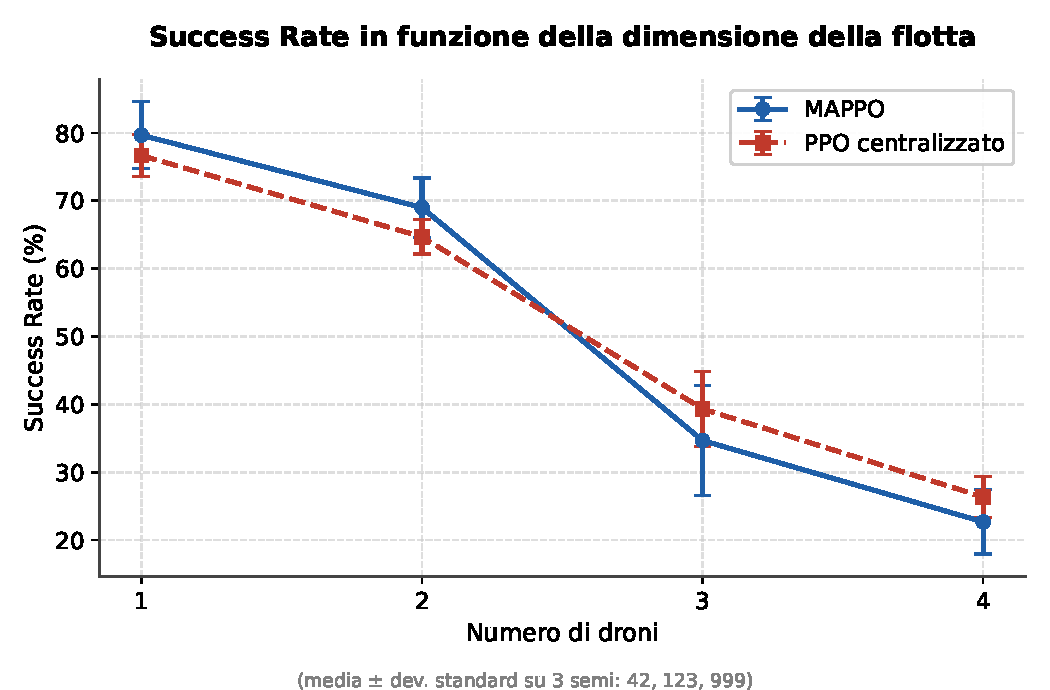
\includegraphics[width=0.8\textwidth]{fig_6_1_success_rate.pdf}
    \caption{Success Rate in funzione del numero di droni.}
    \label{fig:6_1}
\end{figure}

\begin{figure}[htbp]
    \centering
    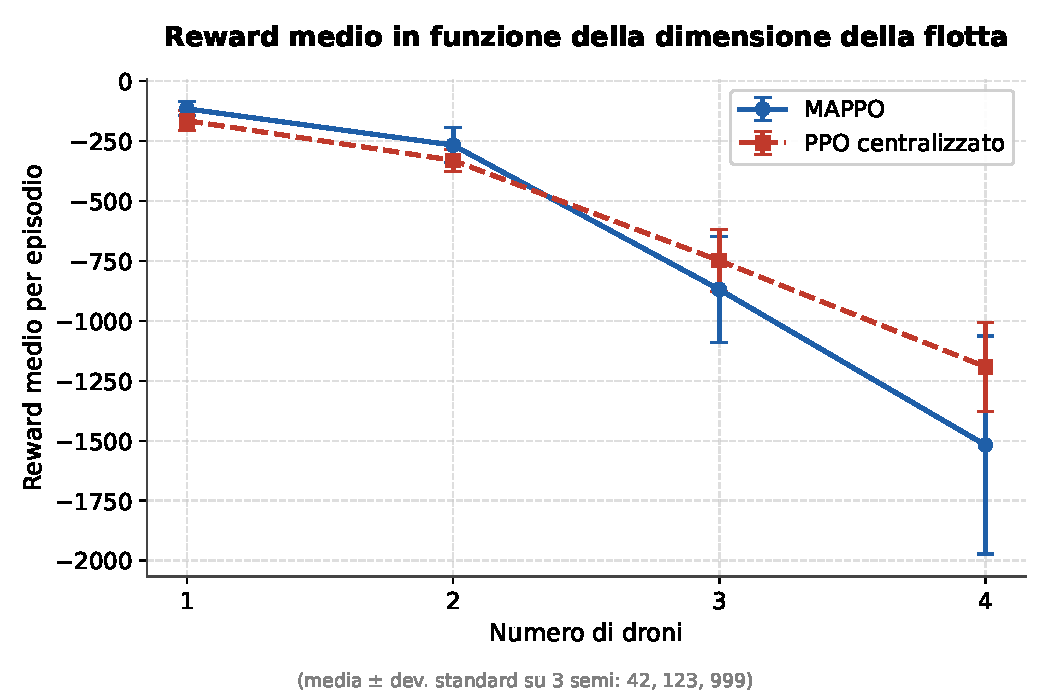
\includegraphics[width=0.8\textwidth]{fig_6_2_reward.pdf}
    \caption{Reward medio in funzione del numero di droni.}
    \label{fig:6_2}
\end{figure}

\begin{figure}[htbp]
    \centering
    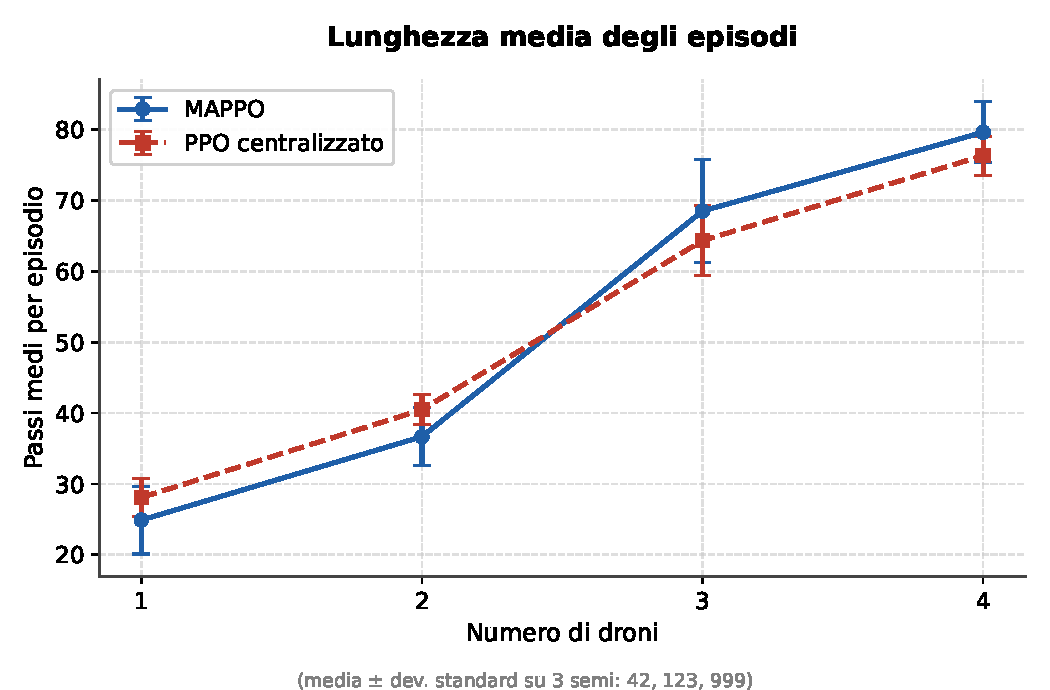
\includegraphics[width=0.8\textwidth]{fig_6_3_passi_medi.pdf}
    \caption{Lunghezza media degli episodi.}
    \label{fig:6_3}
\end{figure}

\paragraph{Andamento con la dimensione della flotta.} Per entrambi gli algoritmi il tasso di successo diminuisce in modo monotono all'aumentare dei droni: da $79,7\%$ a $22,7\%$ per MAPPO e da $76,7\%$ a $26,3\%$ per PPO. Il calo più marcato si registra tra due e tre droni (circa $34$ punti percentuali per MAPPO e $25$ per PPO). Un risultato di squadra richiede che tutti gli $N$ droni raggiungano l'hangar, per cui ogni drone aggiuntivo introduce nuove occasioni di conflitto in prossimità del bersaglio.

\paragraph{Confronto tra gli algoritmi.} MAPPO ottiene un tasso di successo più elevato con uno e due droni ($79,7\%$ contro $76,7\%$ e $69,0\%$ contro $64,7\%$) e un reward medio superiore ($-115,6$ contro $-165,3$ e $-267,0$ contro $-330,7$). Con tre e quattro droni l'ordine si inverte: PPO ottiene il $39,3\%$ contro il $34,7\%$ di MAPPO e il $26,3\%$ contro il $22,7\%$, con un reward migliore. Le differenze vanno però lette con cautela. Gli scarti (da $3$ a $4,7$ punti) sono dello stesso ordine della dispersione tra i semi e dell'errore standard sulla differenza, circa $4$ punti su $300$ episodi, e la loro direzione non è concorde in tutti i semi (Figura~\ref{fig:6_4}). Con soli tre semi, quindi, le differenze non sono significative.

\begin{figure}[htbp]
    \centering
    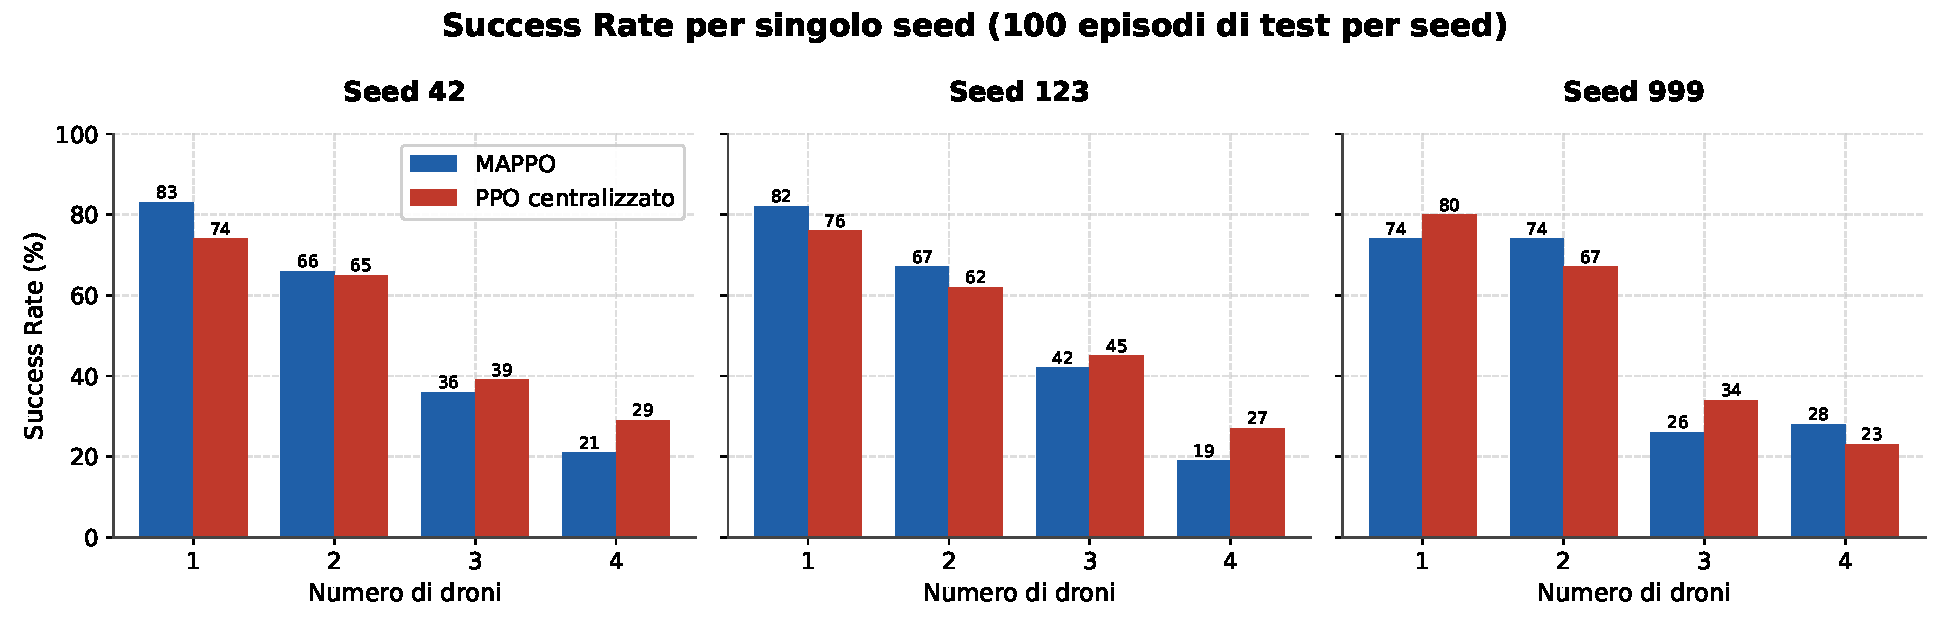
\includegraphics[width=0.95\textwidth]{fig_6_4_success_rate_per_seme.pdf}
    \caption{Success Rate per singolo seed.}
    \label{fig:6_4}
\end{figure}

\paragraph{Reward.} I valori del reward medio sono sempre negativi, anche con un tasso di successo prossimo all'$80\%$, e la loro dispersione è ampia (fino a $\pm 454,5$ a quattro droni con MAPPO). La causa è la struttura della ricompensa: un episodio fallito, in cui un drone rimane bloccato contro una montagna, accumula una penalità di $-10$ a ogni passo per oltre cento passi, e pochi episodi di questo tipo bastano a portare la media in territorio negativo. A titolo di esempio, l'analisi di scomposizione della ricompensa (\texttt{analisi\_reward.py}) applicata al modello MAPPO a un drone del seme $42$, su $100$ nuovi episodi di test, fornisce un tasso di successo del $75\%$. I $75$ episodi riusciti durano in media $5,8$ passi, senza urti, con una ricompensa di circa $+95,2$; i $25$ episodi falliti esauriscono i $100$ passi oscillando contro le montagne, con circa $96$ urti ciascuno, per una ricompensa di circa $-1060$. La media pesata, $0,75 \cdot (+95,2) + 0,25 \cdot (-1060) \approx -193,6$, coincide con il valore misurato di $-194,0$. La linea di base PPO, nelle stesse condizioni, mostra la stessa dinamica ($73\%$ di successo, reward medio $-209,2$, circa $25$ urti contro gli ostacoli per episodio in media). La sequenza di episodi è diversa da quella del benchmark, il che spiega lo scarto rispetto al valore per seme della Figura~\ref{fig:6_4}. Il reward è quindi una misura dominata dai fallimenti, più che dall'efficienza degli episodi riusciti.

\paragraph{Passi medi.} La lunghezza media è calcolata su tutti i $100$ episodi di valutazione, compresi quelli falliti, che terminano per troncamento a $100$ passi. Per questo cresce con il numero di droni (da circa $25$--$28$ passi a un drone a circa $76$--$80$ a quattro). Con quattro droni la maggioranza degli episodi termina per timeout.

\section{Costo computazionale}
\label{sec:costo_computazionale}

La Tabella~\ref{tab:6_2} riporta tempo di addestramento, throughput e risorse impegnate, e le Figure~\ref{fig:6_5} e \ref{fig:6_6} ne mostrano l'andamento.

\begin{table}[htbp]
    \centering
    \resizebox{\textwidth}{!}{%
    \begin{tabular}{clcccc}
        \toprule
        \textbf{Droni} & \textbf{Algoritmo} & \textbf{Tempo (s)} & \textbf{Throughput (passi/s)} & \textbf{CPU media (\%)} & \textbf{RAM (MB)} \\
        \midrule
        1 & MAPPO & $68,3 \pm 1,0$     & $2.196 \pm 33$ & $724,9 \pm 3,1$ & $340,6 \pm 0,5$ \\
        1 & PPO   & $70,0 \pm 0,4$     & $2.144 \pm 11$ & $532,8 \pm 1,3$ & $341,6 \pm 0,5$ \\
        2 & MAPPO & $308,8 \pm 4,0$    & $1.457 \pm 19$ & $798,9 \pm 0,7$ & $343,2 \pm 0,5$ \\
        2 & PPO   & $252,1 \pm 0,1$    & $1.785 \pm 1$  & $482,9 \pm 1,0$ & $342,3 \pm 0,5$ \\
        3 & MAPPO & $673,0 \pm 1,6$    & $1.114 \pm 3$  & $799,5 \pm 0,1$ & $344,7 \pm 0,4$ \\
        3 & PPO   & $486,7 \pm 4,1$    & $1.541 \pm 13$ & $451,1 \pm 0,3$ & $344,1 \pm 0,4$ \\
        4 & MAPPO & $1.254,8 \pm 121,2$ & $802 \pm 81$   & $798,8 \pm 0,9$ & $345,9 \pm 0,5$ \\
        4 & PPO   & $820,2 \pm 2,8$    & $1.219 \pm 4$  & $436,9 \pm 0,6$ & $344,7 \pm 0,6$ \\
        \bottomrule
    \end{tabular}%
    }
    \caption{Costo computazionale dell'addestramento (media $\pm$ deviazione standard su 3 semi).}
    \label{tab:6_2}
\end{table}

\begin{figure}[htbp]
    \centering
    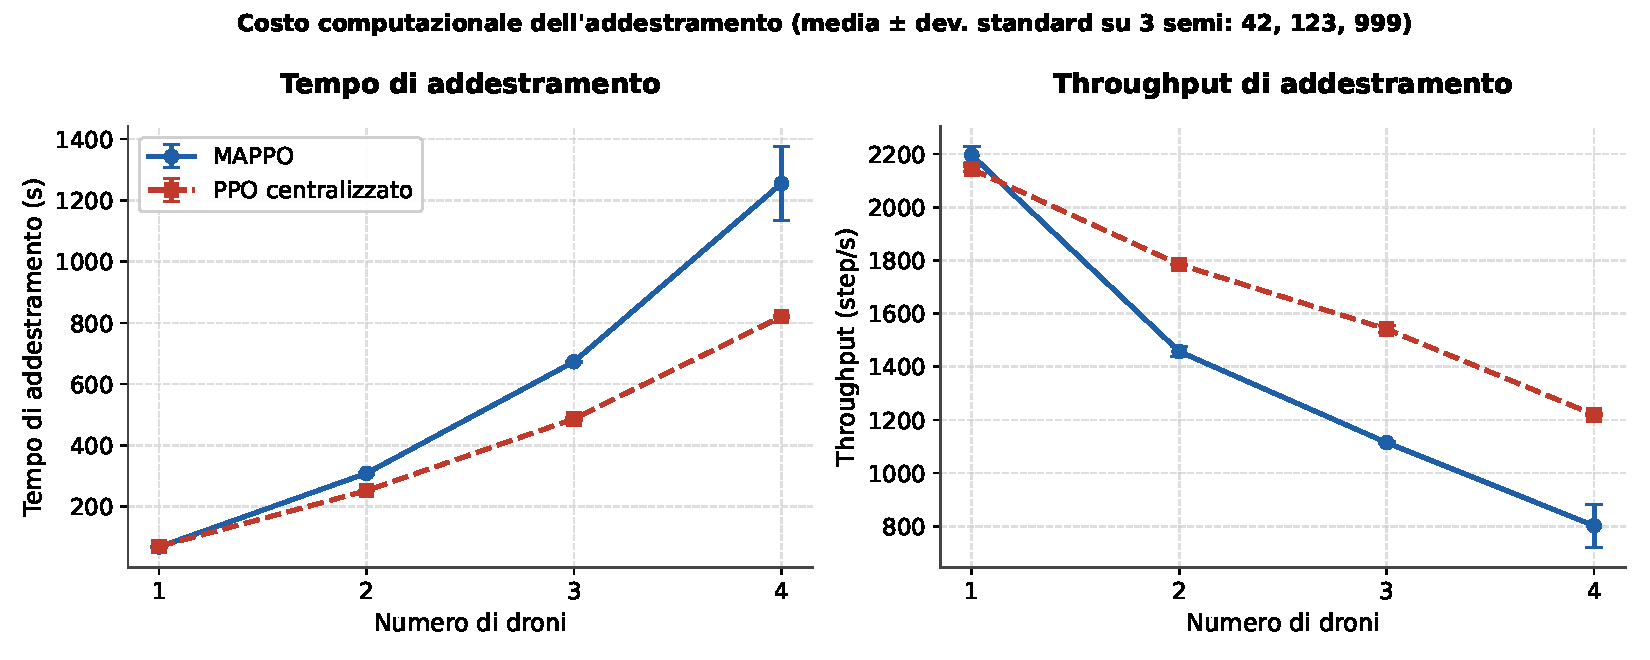
\includegraphics[width=0.95\textwidth]{fig_6_5_tempo_throughput.pdf}
    \caption{Tempo di addestramento e throughput.}
    \label{fig:6_5}
\end{figure}

\begin{figure}[htbp]
    \centering
    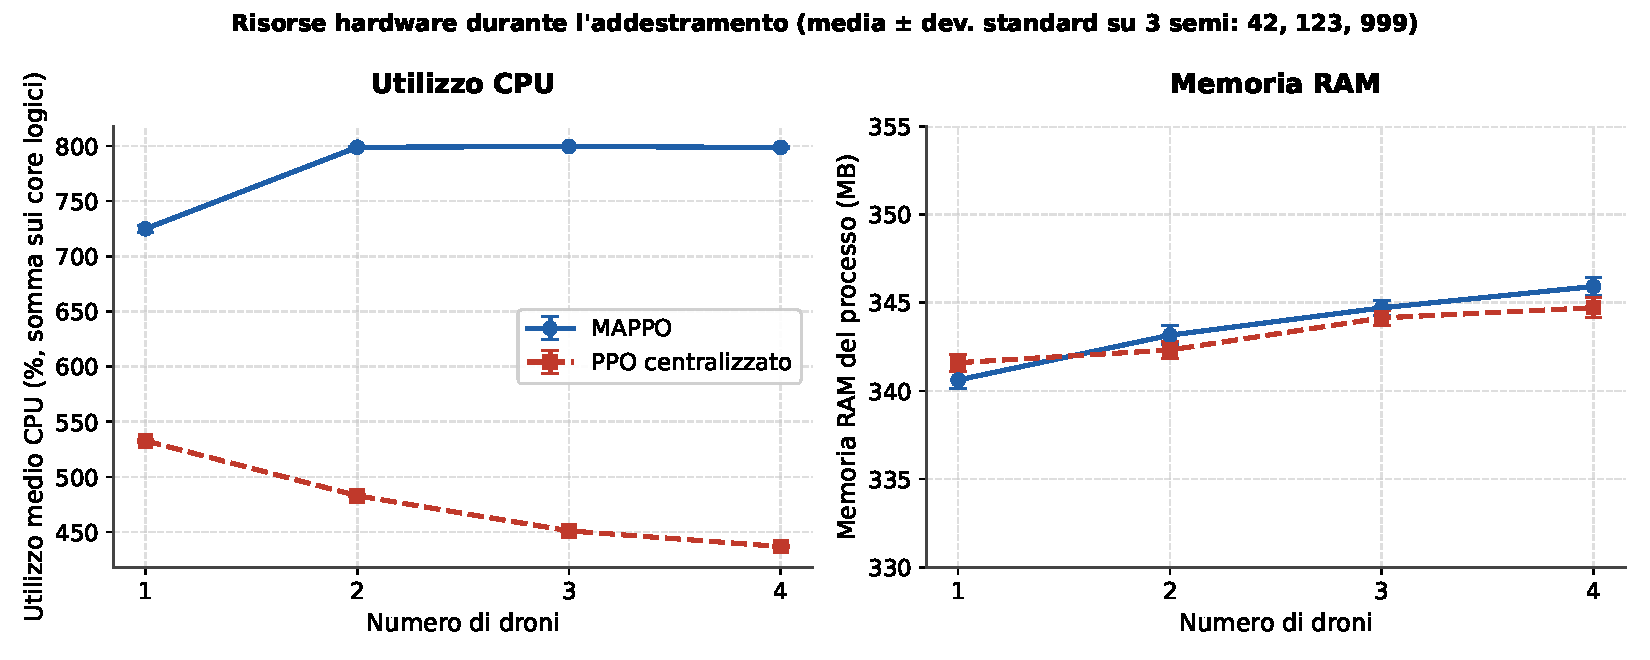
\includegraphics[width=0.95\textwidth]{fig_6_6_risorse_cpu_ram.pdf}
    \caption{Utilizzo di CPU e RAM.}
    \label{fig:6_6}
\end{figure}

Con un drone i due algoritmi hanno tempi e throughput equivalenti ($68,3\text{ s}$ contro $70,0\text{ s}$). Da due droni in poi MAPPO risulta più lento: a tre droni $673,0\text{ s}$ contro $486,7\text{ s}$, a quattro $1.254,8\text{ s}$ contro $820,2\text{ s}$, con un throughput che scende da $2.196$ a $802$ passi al secondo ($-63\%$) contro il calo da $2.144$ a $1.219$ ($-43\%$) di PPO. La crescita dei tempi dipende da due fattori: l'aumento del budget di passi (da $150.000$ a $1.000.000$) e la diminuzione del throughput con $N$. Il maggior costo di MAPPO è verosimilmente legato all'elaborazione per agente dell'actor condiviso, che per aggiornamento tratta $1024 \cdot N$ campioni e un critic distinto, mentre PPO aggiorna una sola rete su $2048$ campioni. A quattro droni la variabilità tra semi dei tempi di MAPPO è più elevata.

L'utilizzo della CPU di MAPPO si assesta su circa $800\%$ a partire da due droni (saturazione degli otto core fisici), mentre PPO impegna $440$--$530\%$. La RAM è praticamente indipendente dalla dimensione della flotta (da $340$ a $346\text{ MB}$, variazione inferiore al $2\%$). L'utilizzo medio della GPU è marginale in tutte le configurazioni (inferiore al $16\%$), come è lecito attendersi da reti di piccole dimensioni in un carico limitato dalla simulazione dell'ambiente.

\section{Calibrazione dei budget di addestramento}
\label{sec:calibrazione_budget}

I budget del confronto principale derivano da run esplorative registrate con TensorBoard per i tre semi. Le metriche sono medie mobili sugli ultimi $100$ episodi, ottenute con policy stocastica, e i valori riportati sono estratti direttamente dai log. Il tasso di successo in addestramento è disponibile solo per MAPPO, e per tre e quattro droni le curve di calibrazione sono disponibili solo per MAPPO; il confronto tra le curve dei due algoritmi a quattro droni è condotto nello studio a $4.000.000$ di passi. Per PPO l'entropia è riportata per drone, dividendo per $N$ l'entropia della distribuzione multicategorica, che è la somma delle entropie delle $N$ componenti: in questo modo è confrontabile con quella di MAPPO. Il valore massimo per cinque azioni è $\ln 5 \approx 1,61$.

\paragraph{Un drone (run a 200.000 passi).} MAPPO raggiunge rapidamente il successo in addestramento: il $95\%$ è superato a $20.480$ passi nei semi $123$ e $999$ e a $40.960$ nel seme $42$, e il $100\%$ è toccato a $20.480$ passi nei primi due e a $81.920$ nel terzo (Figura~\ref{fig:5_1}). Il reward di picco ($+78,20$, $+88,46$ e $+77,42$) avviene tra $61.440$ e $184.320$ passi. Nel tratto successivo il tasso di successo resta tra il $97$ e il $99\%$, mentre il reward diminuisce fino a $+31,77$, $+57,63$ e $+33,73$ a $200.000$ passi: a successo invariato, il calo indica episodi più lunghi o con più urti. PPO converge più lentamente, con picchi tra $+84,30$ e $+85,92$ a $133.120$--$186.368$ passi e valori finali tra $+65,52$ e $+75,25$. Le curve sono riportate nella Figura~\ref{fig:6_7}.

\begin{table}[htbp]
    \centering
    \begin{tabular}{clcc}
        \toprule
        \textbf{Seme} & \textbf{Algoritmo} & \textbf{Reward di picco (passo)} & \textbf{Reward a fine run} \\
        \midrule
        42  & MAPPO & $+78,20$ ($81.920$)  & $+31,77$ ($200.000$) \\
        123 & MAPPO & $+88,46$ ($61.440$)  & $+57,63$ ($200.000$) \\
        999 & MAPPO & $+77,42$ ($184.320$) & $+33,73$ ($200.000$) \\
        42  & PPO   & $+84,30$ ($133.120$) & $+65,52$ ($200.704$) \\
        123 & PPO   & $+85,92$ ($186.368$) & $+67,88$ ($200.704$) \\
        999 & PPO   & $+85,58$ ($137.216$) & $+75,25$ ($200.704$) \\
        \bottomrule
    \end{tabular}
    \caption{Reward medio di addestramento a un drone: picco e valore finale (run a 200.000 passi).}
    \label{tab:6_3}
\end{table}

\begin{figure}[htbp]
    \centering
    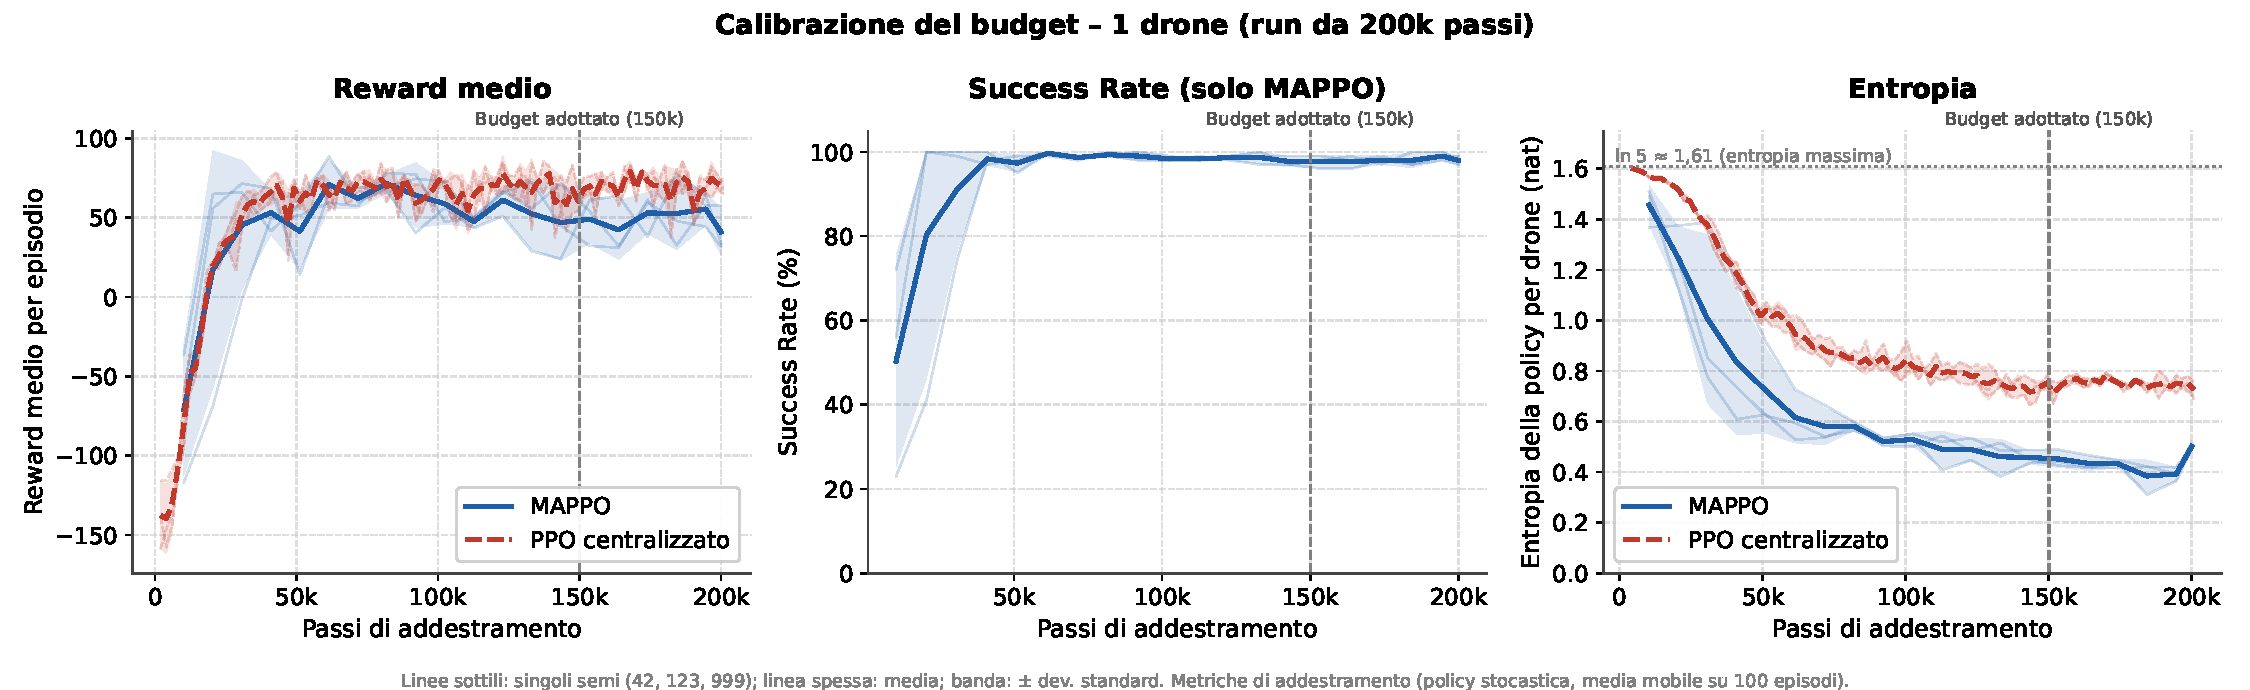
\includegraphics[width=0.95\textwidth]{fig_6_7_calibrazione_1uav.pdf}
    \caption{Calibrazione a un drone: reward medio (MAPPO e PPO), Success Rate (MAPPO) ed entropia per drone, tre semi.}
    \label{fig:6_7}
\end{figure}

\paragraph{Due droni (run a 500.000 passi).} MAPPO supera il $95\%$ di successo già tra $30.720$ e $51.200$ passi, con un massimo del $99\%$ nei semi $42$ e $123$ e del $100\%$ nel seme $999$, e raggiunge il picco di reward tra $61.440$ e $143.360$ passi (Tabella~\ref{tab:6_4}). Oltre questo punto il reward diminuisce in modo progressivo e marcato, fino a $-119,67$, $+2,90$ e $-49,70$ a $500.000$ passi, mentre il successo scende all'$83$--$90\%$ e l'entropia a $0,26$--$0,38$. PPO segue un andamento opposto: converge lentamente, con picchi tra $+155,51$ e $+161,26$ a $409.600$--$489.472$ passi, e mantiene a fine run valori elevati ($+103,51$, $+145,51$ e $+145,86$), con un'entropia per drone tra $0,87$ e $0,92$. Anche il budget di $450.000$ passi è un compromesso: consente a PPO di avvicinarsi al proprio plateau, ma interviene quando MAPPO ha superato il picco da oltre $300.000$ passi (Figura~\ref{fig:6_8}).

\begin{figure}[htbp]
    \centering
    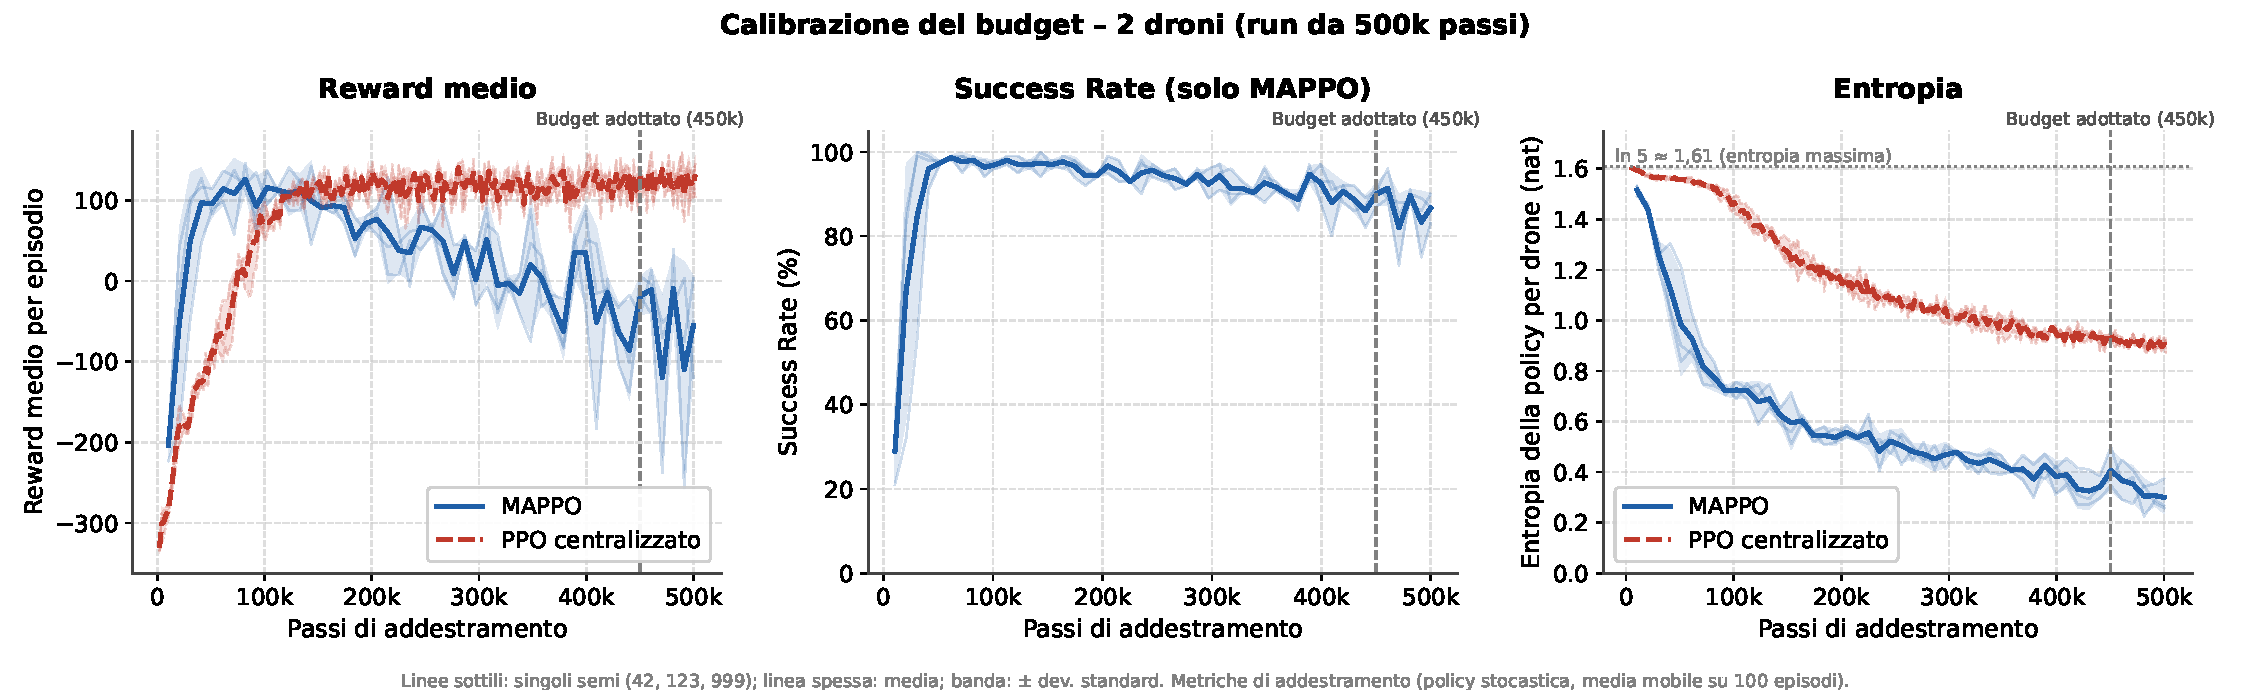
\includegraphics[width=0.95\textwidth]{fig_6_8_calibrazione_2uav.pdf}
    \caption{Calibrazione a due droni: reward medio, Success Rate (MAPPO) ed entropia per drone, tre semi.}
    \label{fig:6_8}
\end{figure}

\paragraph{Tre e quattro droni.} A tre droni MAPPO supera il $95\%$ di successo tra $51.200$ e $71.680$ passi e raggiunge il picco di reward tra $92.160$ e $122.880$ passi; a fine run ($750.000$ passi) il successo di addestramento è sceso al $58$--$65\%$ e il reward a valori tra $-274$ e $-342$, con un'entropia minima di $0,09$--$0,19$. A quattro droni il picco è più tardivo e più basso: il successo massimo è del $98$, $98$ e $92\%$ nei tre semi, tra $102.400$ e $215.040$ passi, e nel seme $999$ non raggiunge mai il $95\%$. A $1.000.000$ di passi il successo di addestramento è sceso al $55$--$64\%$ e il reward a valori tra $-384$ e $-636$ (Tabella~\ref{tab:6_4} e Figura~\ref{fig:6_9}).

\begin{table}[htbp]
    \centering
    \resizebox{\textwidth}{!}{%
    \begin{tabular}{ccccccc}
        \toprule
        \textbf{Droni} & \textbf{Seme} & \textbf{Success Rate max (passo)} & \textbf{Reward di picco (passo)} & \textbf{Reward a fine run} & \textbf{Success Rate a fine run} & \textbf{Entropia a fine run} \\
        \midrule
        2 & 42  & $99\%$ ($30.720$)  & $+136,45$ ($61.440$)  & $-119,67$ & $87\%$ & $0,27$ \\
        2 & 123 & $99\%$ ($61.440$)  & $+146,41$ ($81.920$)  & $+2,90$   & $90\%$ & $0,38$ \\
        2 & 999 & $100\%$ ($30.720$) & $+142,26$ ($143.360$) & $-49,70$  & $83\%$ & $0,26$ \\
        \midrule
        3 & 42  & $99\%$ ($122.880$) & $+196,58$ ($122.880$) & $-274,05$ & $64\%$ & $0,26$ \\
        3 & 123 & $99\%$ ($71.680$)  & $+176,82$ ($122.880$) & $-336,28$ & $65\%$ & $0,56$ \\
        3 & 999 & $100\%$ ($51.200$) & $+197,33$ ($92.160$)  & $-342,09$ & $58\%$ & $0,24$ \\
        \midrule
        4 & 42  & $98\%$ ($184.320$) & $+163,73$ ($184.320$) & $-635,72$ & $57\%$ & $0,29$ \\
        4 & 123 & $98\%$ ($102.400$) & $+188,31$ ($112.640$) & $-384,00$ & $55\%$ & $0,46$ \\
        4 & 999 & $92\%$ ($215.040$) & $+109,40$ ($215.040$) & $-626,06$ & $64\%$ & $0,29$ \\
        \bottomrule
    \end{tabular}%
    }
    \caption{Curve di addestramento di MAPPO da due a quattro droni: picco e valori a fine run (500.000, 750.000 e 1.000.000 di passi).}
    \label{tab:6_4}
\end{table}

\begin{figure}[htbp]
    \centering
    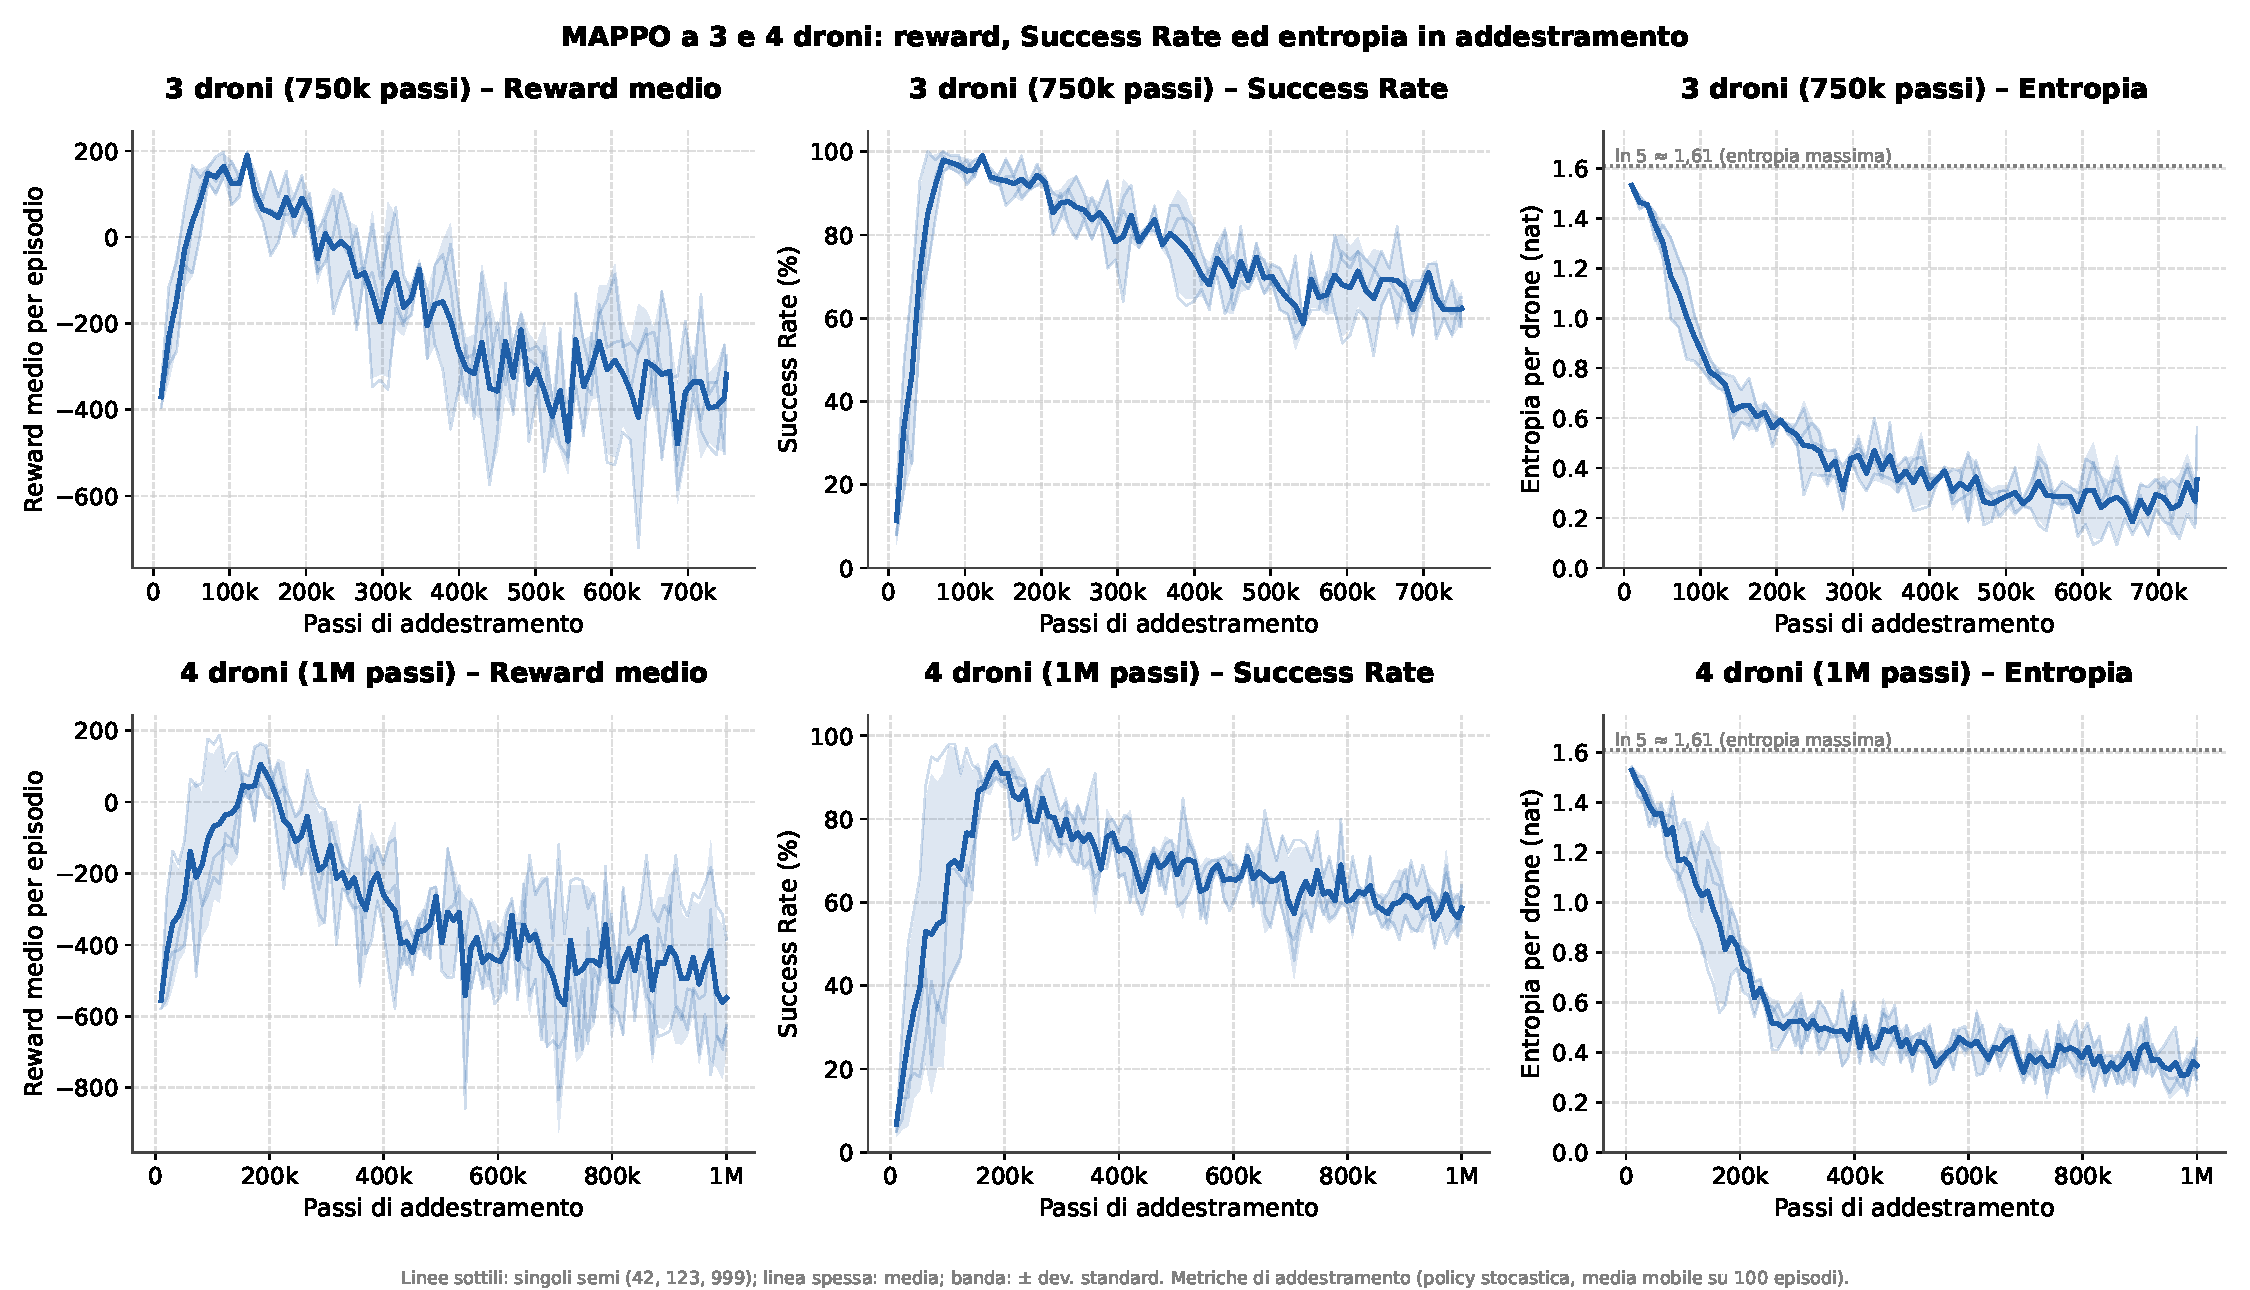
\includegraphics[width=0.95\textwidth]{fig_6_9_mappo_3_4_uav.pdf}
    \caption{MAPPO a tre e quattro droni: reward medio, Success Rate ed entropia in addestramento, tre semi.}
    \label{fig:6_9}
\end{figure}

\paragraph{Divario tra addestramento e valutazione.} Le metriche di addestramento, ottenute campionando le azioni, sono sistematicamente migliori di quelle di valutazione deterministica. A tre droni MAPPO termina l'addestramento con il $58$--$65\%$ di successo, contro il $34,7\%$ in valutazione; a quattro droni con il $55$--$64\%$, contro il $22,7\%$. Per PPO a due droni il reward di fine run è positivo (da $+103,5$ a $+145,9$), mentre quello di valutazione è $-330,7$.La discrepanza è pienamente giustificata dal passaggio dal campionamento stocastico alla valutazione puramente deterministica .

\section{Prove preliminari con PPO}
\label{sec:prove_preliminari}

Le prime sperimentazioni, condotte con PPO, avevano l'obiettivo di stimare il budget di addestramento (Figura~\ref{fig:6_10}).
\begin{itemize}
    \item \textbf{Un drone, 50.000 passi, senza ostacoli (51.200 effettivi).} L'agente converge in meno di $20.000$ passi: il reward diventa positivo già a $8.192$ passi e raggiunge $+93,61$ a fine run, con episodi di $6,39$ passi in media.
    \item \textbf{Un drone, 50.000 passi, con quattro ostacoli.} Il reward cresce più lentamente e a fine run vale $+10,20$ (picco di $+15,19$ a $47.104$ passi), con episodi di $38,6$ passi in media: il budget non basta in presenza di ostacoli e la curva è ancora in crescita.
    \item \textbf{Un drone, 500.000 passi, con quattro ostacoli (501.760 effettivi).} Il reward diventa positivo a $24.576$ passi e si stabilizza attorno a $+65$/$+80$ da circa $80.000$ passi, con episodi di $9$--$11$ passi. Il picco di $+86,05$ ($403.456$ passi) e il valore finale di $+57,13$ sono oscillazioni attorno a questo plateau: oltre la convergenza, ulteriori passi non producono miglioramenti.
\end{itemize}

Nella prima versione dell'ambiente multi-agente, PPO a due droni con seme $42$ è stato addestrato con $1.000.000$ ($1.001.472$ effettivi) e $1.500.000$ passi ($1.501.184$ effettivi). Il reward diventa positivo a $86.016$ e $73.728$ passi e si stabilizza tra $+100$ e $+150$ da circa $200.000$ passi. I picchi sono di $+162,02$ ($952.320$ passi, $11,98$ passi medi) e $+173,74$ ($1.411.072$ passi, $10,61$ passi medi), i valori finali di $+121,11$ e $+144,80$. Le due curve sono quasi sovrapposte, per cui l'aumento del budget da $1.000.000$ a $1.500.000$ passi produce solo un guadagno marginale.

\begin{figure}[htbp]
    \centering
    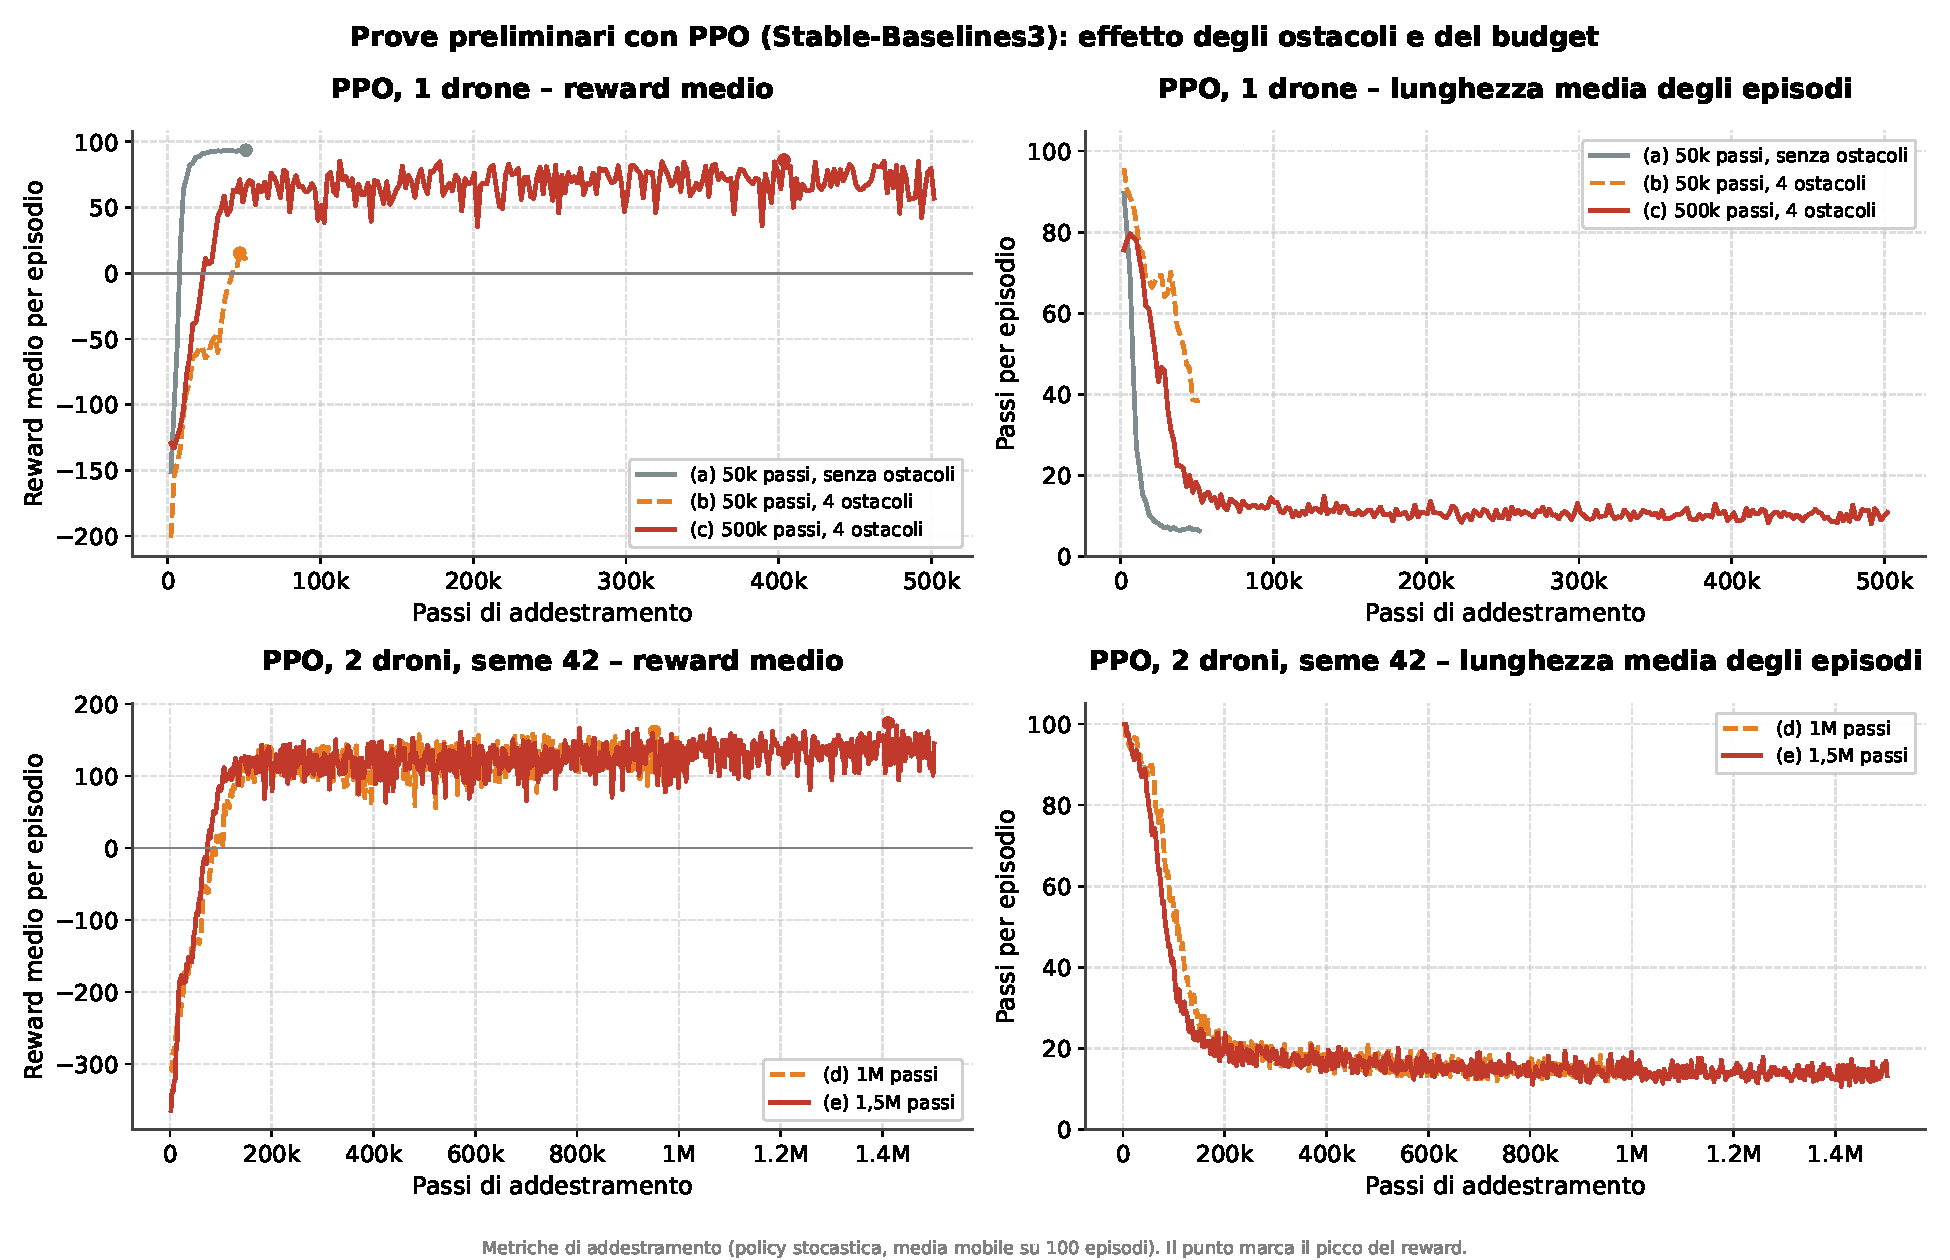
\includegraphics[width=0.95\textwidth]{fig_6_10_preliminari_ppo.pdf}
    \caption{Prove preliminari con PPO: reward medio e lunghezza degli episodi a un drone (senza ostacoli e con quattro ostacoli) e a due droni (1M e 1,5M passi).}
    \label{fig:6_10}
\end{figure}

% =============================================================================
% CAPITOLO 7 - RISULTATI II: ANALISI E DIAGNOSI A 4 UAV
% =============================================================================
\chapter{Risultati II: analisi e diagnosi a 4 UAV}
\label{chap:risultati_2}

Il capitolo verifica se il basso tasso di successo osservato a quattro droni possa essere risolto aumentando il budget di addestramento, e ne individua le cause attraverso la scomposizione della ricompensa e l'analisi dei casi di stallo. I valori di valutazione sono medie e deviazioni standard campionarie sui tre semi ($42$, $123$, $999$).

\section{Studio a 4.000.000 di passi}
\label{sec:studio_4m}

MAPPO e PPO sono stati riaddestrati a quattro droni con un budget di $4.000.000$ di passi, quattro volte quello del confronto principale. La Tabella~\ref{tab:7_1} riporta i risultati della valutazione deterministica.

\begin{table}[htbp]
    \centering
    \begin{tabular}{lcc}
        \toprule
        \textbf{Metrica} & \textbf{MAPPO} & \textbf{PPO centralizzato} \\
        \midrule
        Success Rate (\%)          & $18,0 \pm 6,6$      & $41,0 \pm 7,5$ \\
        Reward medio               & $-1.083,3 \pm 96,5$ & $-1.011,6 \pm 163,1$ \\
        Passi medi per episodio    & $84,2 \pm 5,8$      & $63,1 \pm 6,7$ \\
        Tempo di addestramento (s) & $5.375,6 \pm 159,9$ & $3.447,1 \pm 67,3$ \\
        Throughput (passi/s)       & $745 \pm 23$        & $1.161 \pm 22$ \\
        CPU media (\%)             & $795,9 \pm 0,2$     & $425,0 \pm 4,6$ \\
        RAM (MB)                   & $354,5 \pm 10,6$    & $355,9 \pm 7,7$ \\
        \bottomrule
    \end{tabular}
    \caption{Confronto a quattro droni con budget di 4.000.000 di passi (media $\pm$ deviazione standard su 3 semi; 100 episodi per seme).}
    \label{tab:7_1}
\end{table}

L'aumento del budget ha effetti opposti sui due algoritmi (Figura~\ref{fig:7_1}). Il tasso di successo di MAPPO non migliora, anzi passa dal $22,7 \pm 4,7\%$ a $1.000.000$ di passi al $18,0 \pm 6,6\%$ ($12$, $25$ e $17\%$ nei tre semi). Quello di PPO sale dal $26,3 \pm 3,1\%$ al $41,0 \pm 7,5\%$ ($42$, $48$ e $33\%$). Raggiunti i $4$ milioni di passi, PPO stacca di $23$ punti: pari a circa tre volte la deviazione standard e confermato su tutti e tre i seed. Il reward medio dei due algoritmi resta invece simile ($-1.083,3$ contro $-1.011,6$) e molto negativo. Sul piano computazionale una run di MAPPO dura in media circa $1$ ora e $30$ minuti e una di PPO circa $57$ minuti (Figura~\ref{fig:7_2}), con un throughput di PPO superiore del $56\%$.

\begin{figure}[htbp]
    \centering
    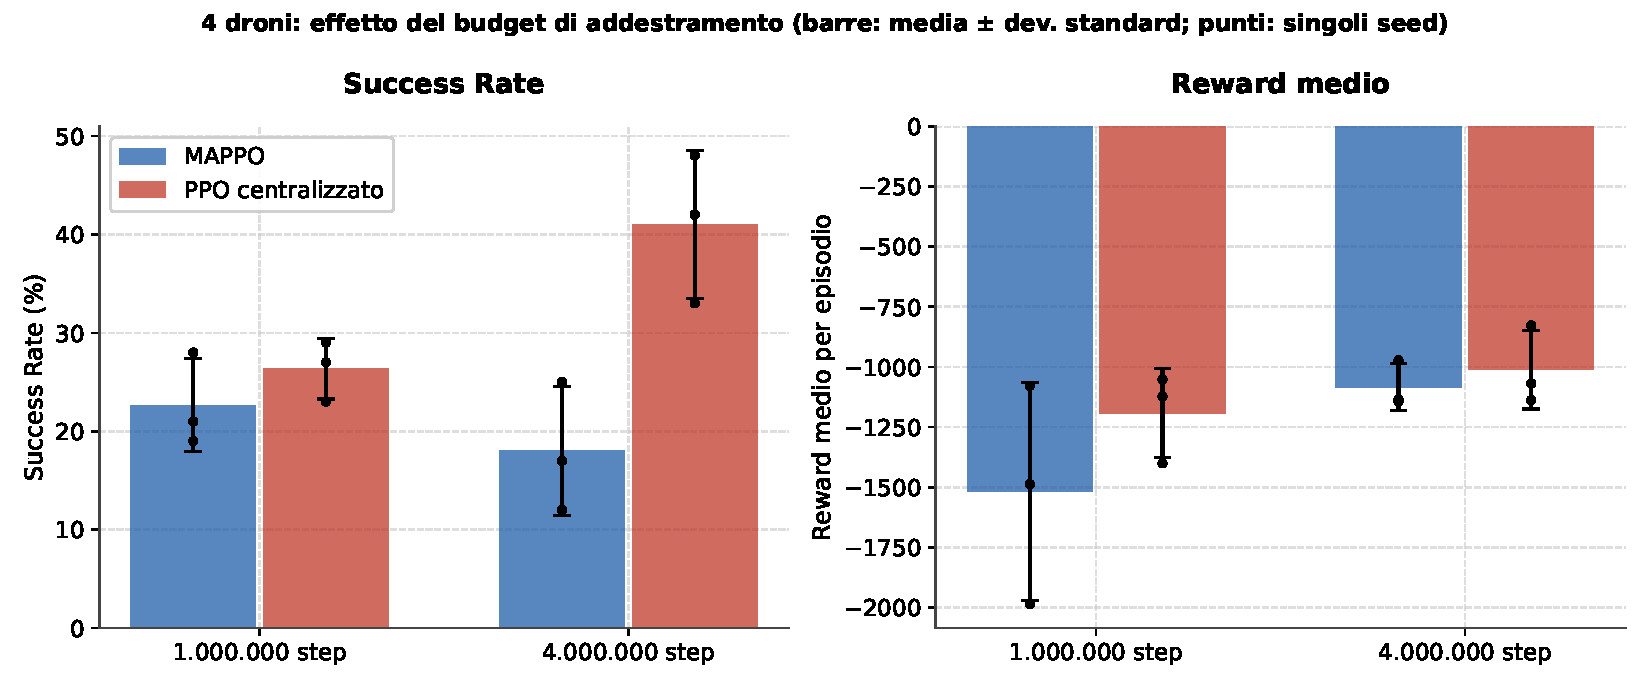
\includegraphics[width=0.95\textwidth]{fig_7_1_4uav_1M_vs_4M.pdf}
    \caption{4 droni: Success Rate e reward medio a 1.000.000 e 4.000.000 di passi (barre: media $\pm$ deviazione standard; punti: singoli semi).}
    \label{fig:7_1}
\end{figure}

\begin{figure}[htbp]
    \centering
    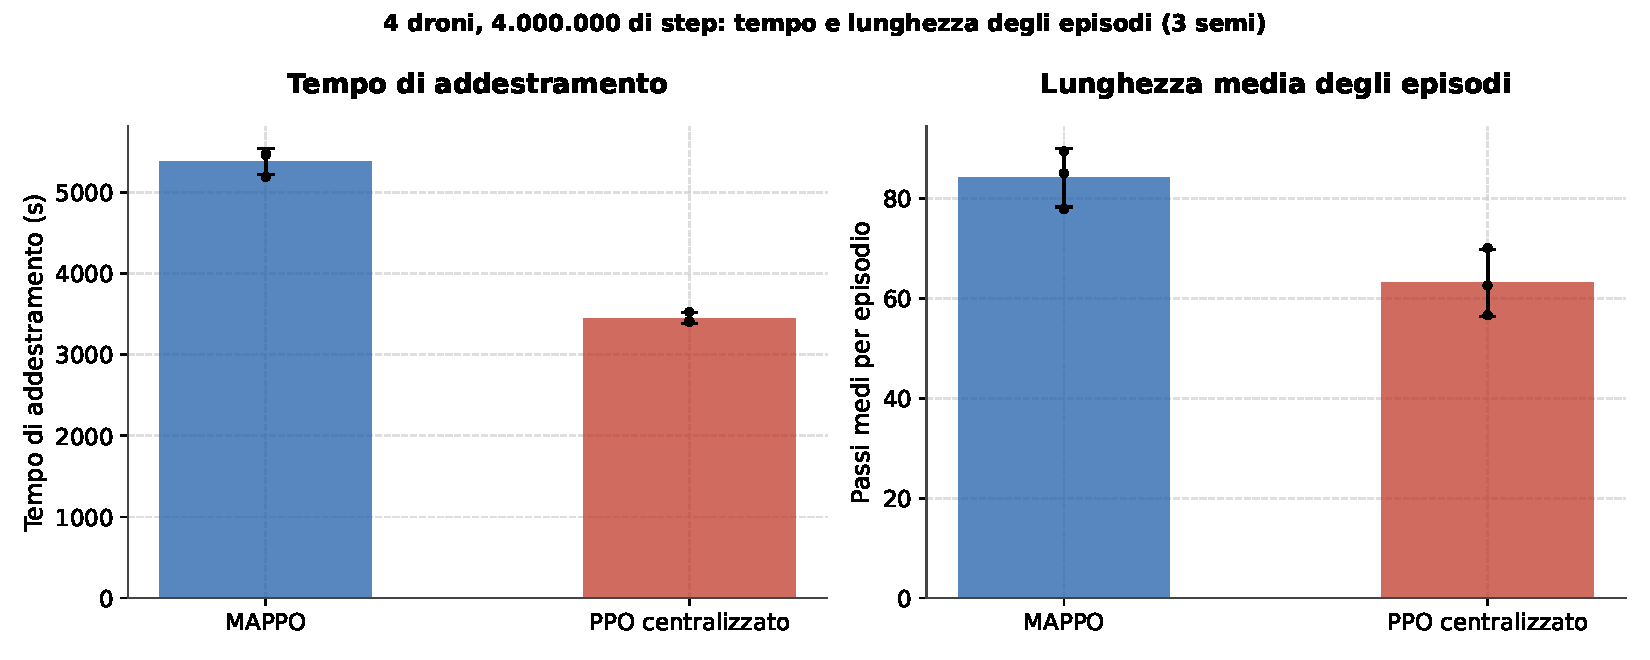
\includegraphics[width=0.95\textwidth]{fig_7_2_4uav_4M_tempo_passi.pdf}
    \caption{4 droni, 4.000.000 di passi: tempo di addestramento e lunghezza media degli episodi.}
    \label{fig:7_2}
\end{figure}

\section{Curve di addestramento a 4.000.000 di passi}
\label{sec:curve_4m}

Le curve di addestramento (Figura~\ref{fig:7_3}) mostrano due dinamiche molto diverse.

\paragraph{MAPPO.} La prestazione massima viene raggiunta presto, tra $102.400$ e $215.040$ passi: il successo in addestramento tocca il $98\%$ nei semi $42$ e $123$ e il $92\%$ nel seme $999$, con reward di picco di $+163,73$, $+188,31$ e $+109,40$. In corrispondenza del picco l'entropia della policy è ancora elevata (tra $0,77$ e $0,94$). Proseguendo l'addestramento, reward e successo diminuiscono e si stabilizzano su valori molto più bassi: nell'ultimo milione di passi il successo medio di addestramento è del $44$--$50\%$ e il reward medio tra $-239$ e $-283$. Parallelamente, l'entropia diminuisce fino ad attestarsi su valori medi di $0,33$--$0,39$ nell'ultimo milione di passi, toccando minimi puntuali di $0,13$--$0,15$ (Figura~\ref{fig:7_4}).

\paragraph{PPO.} Il reward cresce più lentamente, si stabilizza attorno a $+200$ da circa $500.000$ passi e raggiunge i valori massimi molto tardi ($+286,84$, $+291,01$ e $+298,35$, tra $2,94$ e $3,26$ milioni di passi). Nell'ultimo milione di passi il reward medio di addestramento è tra $+210$ e $+226$ e la lunghezza media degli episodi tra $21$ e $22$ passi (Figura~\ref{fig:7_5}). L'entropia per drone, pur in assenza di bonus di entropia, rimane tra $0,91$ e $0,95$ nell'ultimo milione di passi, molto al di sopra di quella di MAPPO.

\begin{figure}[htbp]
    \centering
    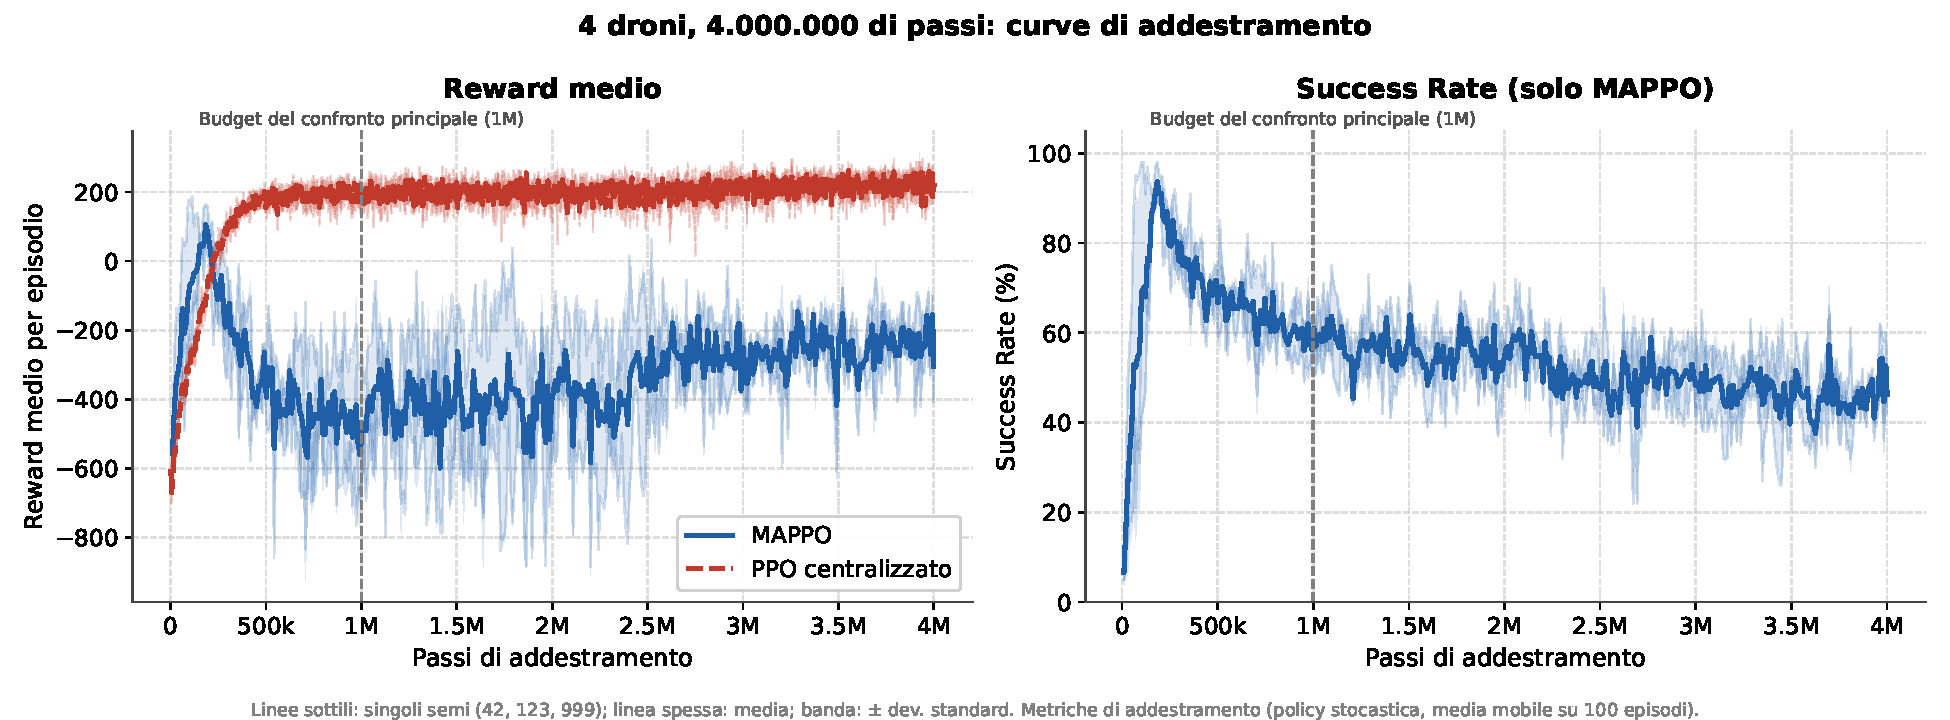
\includegraphics[width=0.95\textwidth]{fig_7_3_4uav_4M_curve.pdf}
    \caption{4 droni, 4.000.000 di passi: reward medio (MAPPO e PPO) e Success Rate (MAPPO) in addestramento.}
    \label{fig:7_3}
\end{figure}

\begin{figure}[htbp]
    \centering
    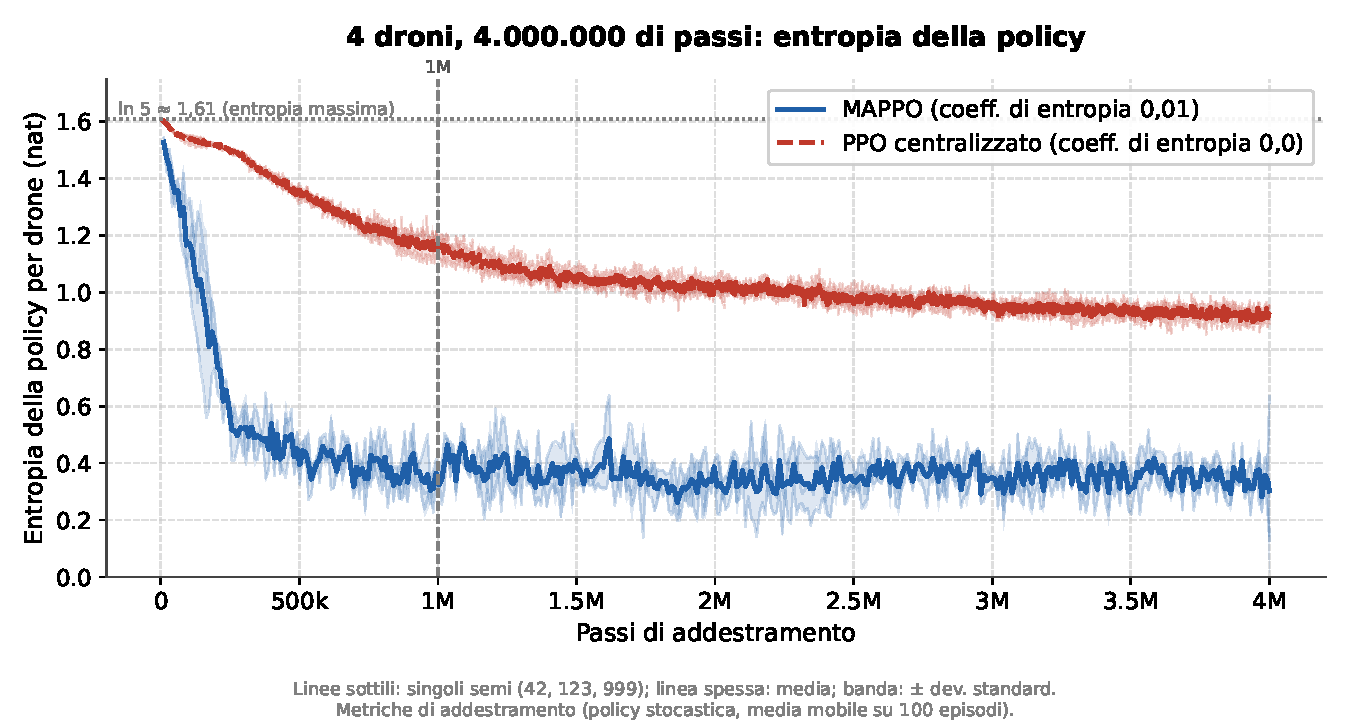
\includegraphics[width=0.9\textwidth]{fig_7_4_4uav_4M_entropia.pdf}
    \caption{4 droni, 4.000.000 di passi: entropia della policy per drone.}
    \label{fig:7_4}
\end{figure}

\begin{figure}[htbp]
    \centering
    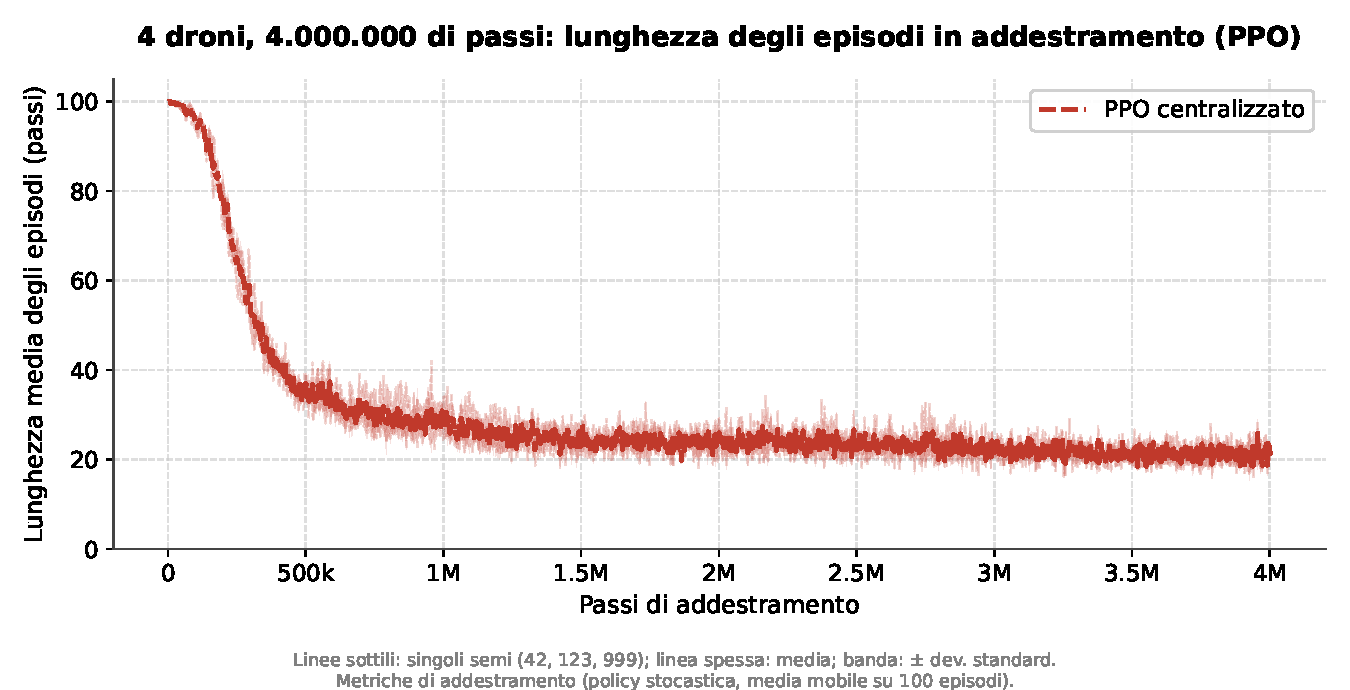
\includegraphics[width=0.9\textwidth]{fig_7_5_4uav_4M_lunghezza_ppo.pdf}
    \caption{4 droni, 4.000.000 di passi: lunghezza media degli episodi in addestramento per PPO.}
    \label{fig:7_5}
\end{figure}

\paragraph{Divario tra addestramento e valutazione.} Per entrambi gli algoritmi le metriche di addestramento sono molto migliori di quelle di valutazione deterministica, e per PPO il divario è particolarmente evidente: in addestramento il reward è positivo (circa $+220$ a fine run) e gli episodi durano $20$--$22$ passi, in valutazione il reward è $-1.011,6$ e gli episodi durano in media $63,1$ passi. Per MAPPO il successo passa dal $44$--$50\%$ di addestramento al $18,0\%$ di valutazione. La policy stocastica consente ai droni di uscire da una situazione di blocco con una scelta diversa da quella più probabile; con la selezione deterministica, invece, un drone la cui azione più probabile è bloccata da un ostacolo o da un compagno ripete la stessa scelta fino al termine dell'episodio.

\section{Scomposizione della ricompensa}
\label{sec:scomposizione_ricompensa}

Il reward medio osservato a $4.000.000$ di passi, $-1.083,3$ per MAPPO e $-1.011,6$ per PPO, è ben inferiore al riferimento di $-400$ in assenza di arrivi e di collisioni: la differenza può derivare solo dalle penalità di collisione. Per quantificarne la composizione è stato sviluppato uno script di analisi (\texttt{analisi\_reward.py}), che esegue $100$ nuovi episodi per ciascun seme con una versione strumentata dell'ambiente e registra separatamente ciascuna voce della ricompensa (Tabella~\ref{tab:7_2}, Figura~\ref{fig:7_6}).

\begin{table}[htbp]
    \centering
    \begin{tabular}{lcc}
        \toprule
        \textbf{Voce (media per episodio)} & \textbf{MAPPO} & \textbf{PPO centralizzato} \\
        \midrule
        Reward totale                              & $-1.118,6 \pm 16,2$      & $-901,7 \pm 75,1$ \\
        Success Rate                               & $16,7\%$                 & $41,0\%$ \\
        Passi medi                                 & $85,3$                   & $63,4$ \\
        Droni atterrati (su 4)                     & $2,03$                   & $2,91$ \\
        Bonus di atterraggio ($+100$)              & $+202,7$                 & $+290,7$ \\
        Penalità temporale ($-1$ per drone in volo) & $-209,3$                 & $-126,9$ \\
        Collisioni tra droni ($-20$)               & $-646,5$ ($32,3$ eventi) & $-473,7$ ($23,7$ eventi) \\
        Urti con ostacoli ($-10$)                  & $-390,7$ ($39,1$ eventi) & $-528,1$ ($52,8$ eventi) \\
        Uscite dai bordi ($-10$)                   & $-74,7$ ($7,5$ eventi)   & $-63,5$ ($6,4$ eventi) \\
        \bottomrule
    \end{tabular}
    \caption{Scomposizione della ricompensa a quattro droni (modelli a 4.000.000 di passi; 100 nuovi episodi per seme, 300 in totale).}
    \label{tab:7_2}
\end{table}

\begin{figure}[htbp]
    \centering
    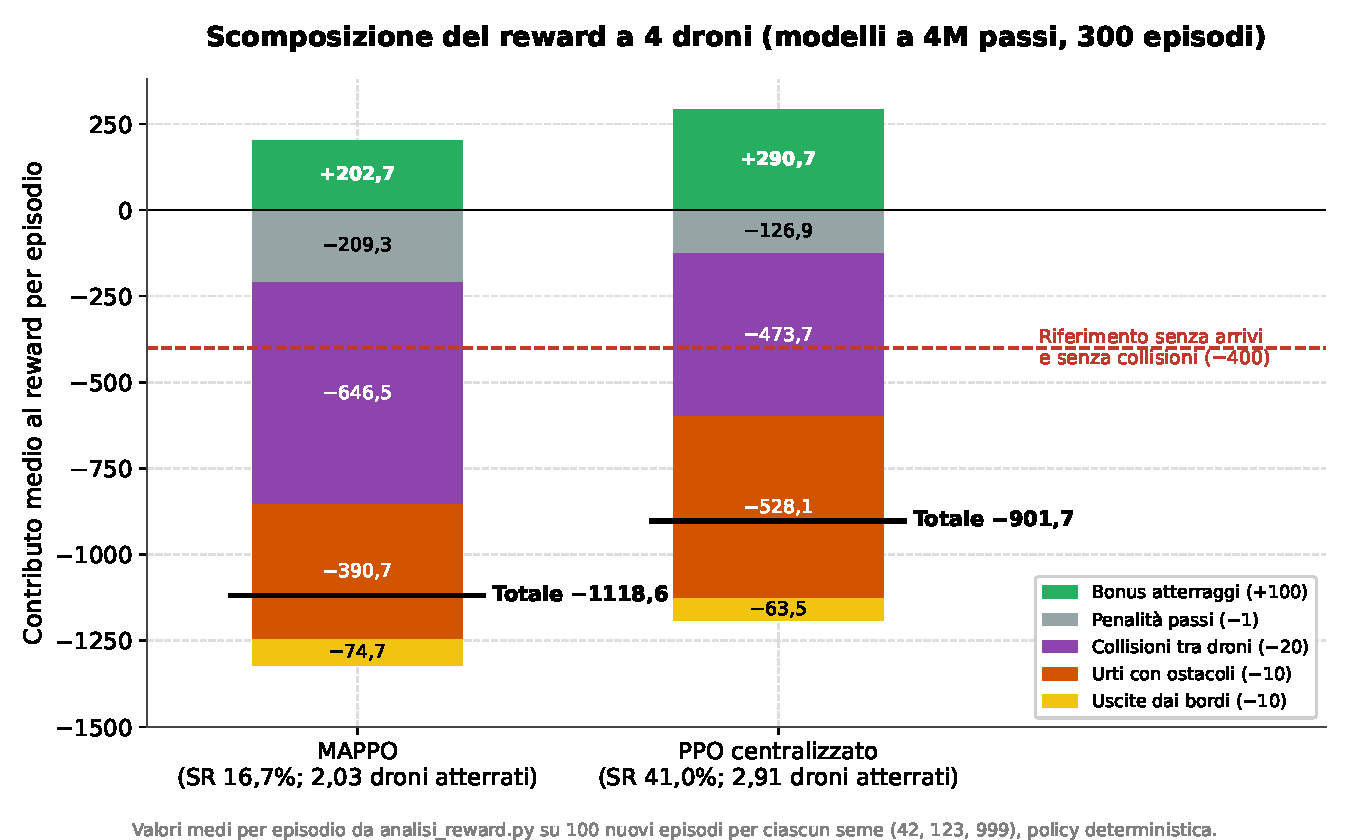
\includegraphics[width=0.95\textwidth]{fig_7_6_scomposizione_ricompensa.pdf}
    \caption{Scomposizione della ricompensa a quattro droni rispetto al riferimento di $-400$.}
    \label{fig:7_6}
\end{figure}

La sequenza di episodi è diversa da quella del benchmark, per cui i valori differiscono leggermente da quelli della Tabella~\ref{tab:7_1}. La scomposizione mette in luce due meccanismi di fallimento distinti. Per MAPPO la voce più pesante sono le collisioni tra droni: $32,3$ eventi per episodio, contro i $23,7$ di PPO, a cui si aggiunge un numero minore di droni atterrati ($2,03$ contro $2,91$). Per PPO prevalgono invece gli urti contro gli ostacoli ($52,8$ eventi per episodio, contro i $39,1$ di MAPPO). In entrambi i casi questi urti sono coerenti con il comportamento osservato a un drone: un drone la cui azione deterministica punta contro una montagna ripete il tentativo a ogni passo, accumulando $-10$ per passo. Il conflitto tra droni è dunque la causa che distingue MAPPO da PPO, mentre il blocco contro gli ostacoli è comune ai due algoritmi.

\section{Il dilemma di coordinazione simmetrica}
\label{sec:dilemma_simmetrico}

Il maggior numero di collisioni tra droni di MAPPO può essere ricondotto al problema della rottura della simmetria nei sistemi multi-agente omogenei. Il meccanismo nasce dalla combinazione di tre fattori.
\begin{itemize}
    \item \textbf{Parametri condivisi e osservazione ego-centrica.} Tutti i droni usano la stessa rete. Due droni in posizioni equivalenti o speculari rispetto all'hangar ricevono osservazioni che, in forma ego-centrica, differiscono poco, e tendono quindi a produrre la stessa decisione: ad esempio, avanzare entrambi verso la stessa cella libera adiacente al bersaglio.
    \item \textbf{Policy quasi deterministica.} Sia in valutazione, deterministica, sia in addestramento, dove l'entropia di MAPPO scende a $0,33$--$0,39$, la policy offre poche occasioni di uscire da un conflitto con una scelta diversa.
    \item \textbf{Regola di blocco.} Una collisione congela entrambi i droni nelle celle di partenza. Al passo successivo la configurazione è identica, la decisione si ripete e la collisione si rinnova, potenzialmente fino al termine dell'episodio.
\end{itemize}

A questi fattori si aggiunge il problema dell'assegnazione del reward: la ricompensa è di squadra e l'advantage è comune a tutti i droni nello stesso passo, per cui la penalità di una collisione tra due droni ricade su tutti e quattro, senza indicare quale dei due avrebbe dovuto cedere il passo.

Il PPO centralizzato non è soggetto allo stesso vincolo. Le uscite dei diversi droni sono distinte, e una stessa configurazione di ingresso può quindi produrre azioni diverse per droni diversi: ad esempio, un drone che avanza mentre gli altri attendono. La sua policy mantiene inoltre un'entropia molto più elevata in addestramento. Il vantaggio di PPO a quattro droni non va però interpretato come prova di una superiorità del paradigma centralizzato: PPO richiede un controllore unico con accesso allo stato globale anche in esecuzione, e le due configurazioni differiscono anche negli iperparametri.

La dipendenza dalla dimensione della flotta è causata perché l'hangar è una singola cella con al più quattro celle adiacenti, e i droni la raggiungono passando da queste ultime. Con due droni restano sempre più celle di accesso libere di quanti siano i droni in arrivo; con quattro droni il numero di accessi è pari a quello dei droni, e basta una montagna vicina all'hangar o al bordo della mappa per rendere impossibile l'accesso simultaneo, imponendo un ordine che le policy, senza una regola esplicita, non riescono a stabilire.

\begin{figure}[htbp]
    \centering
    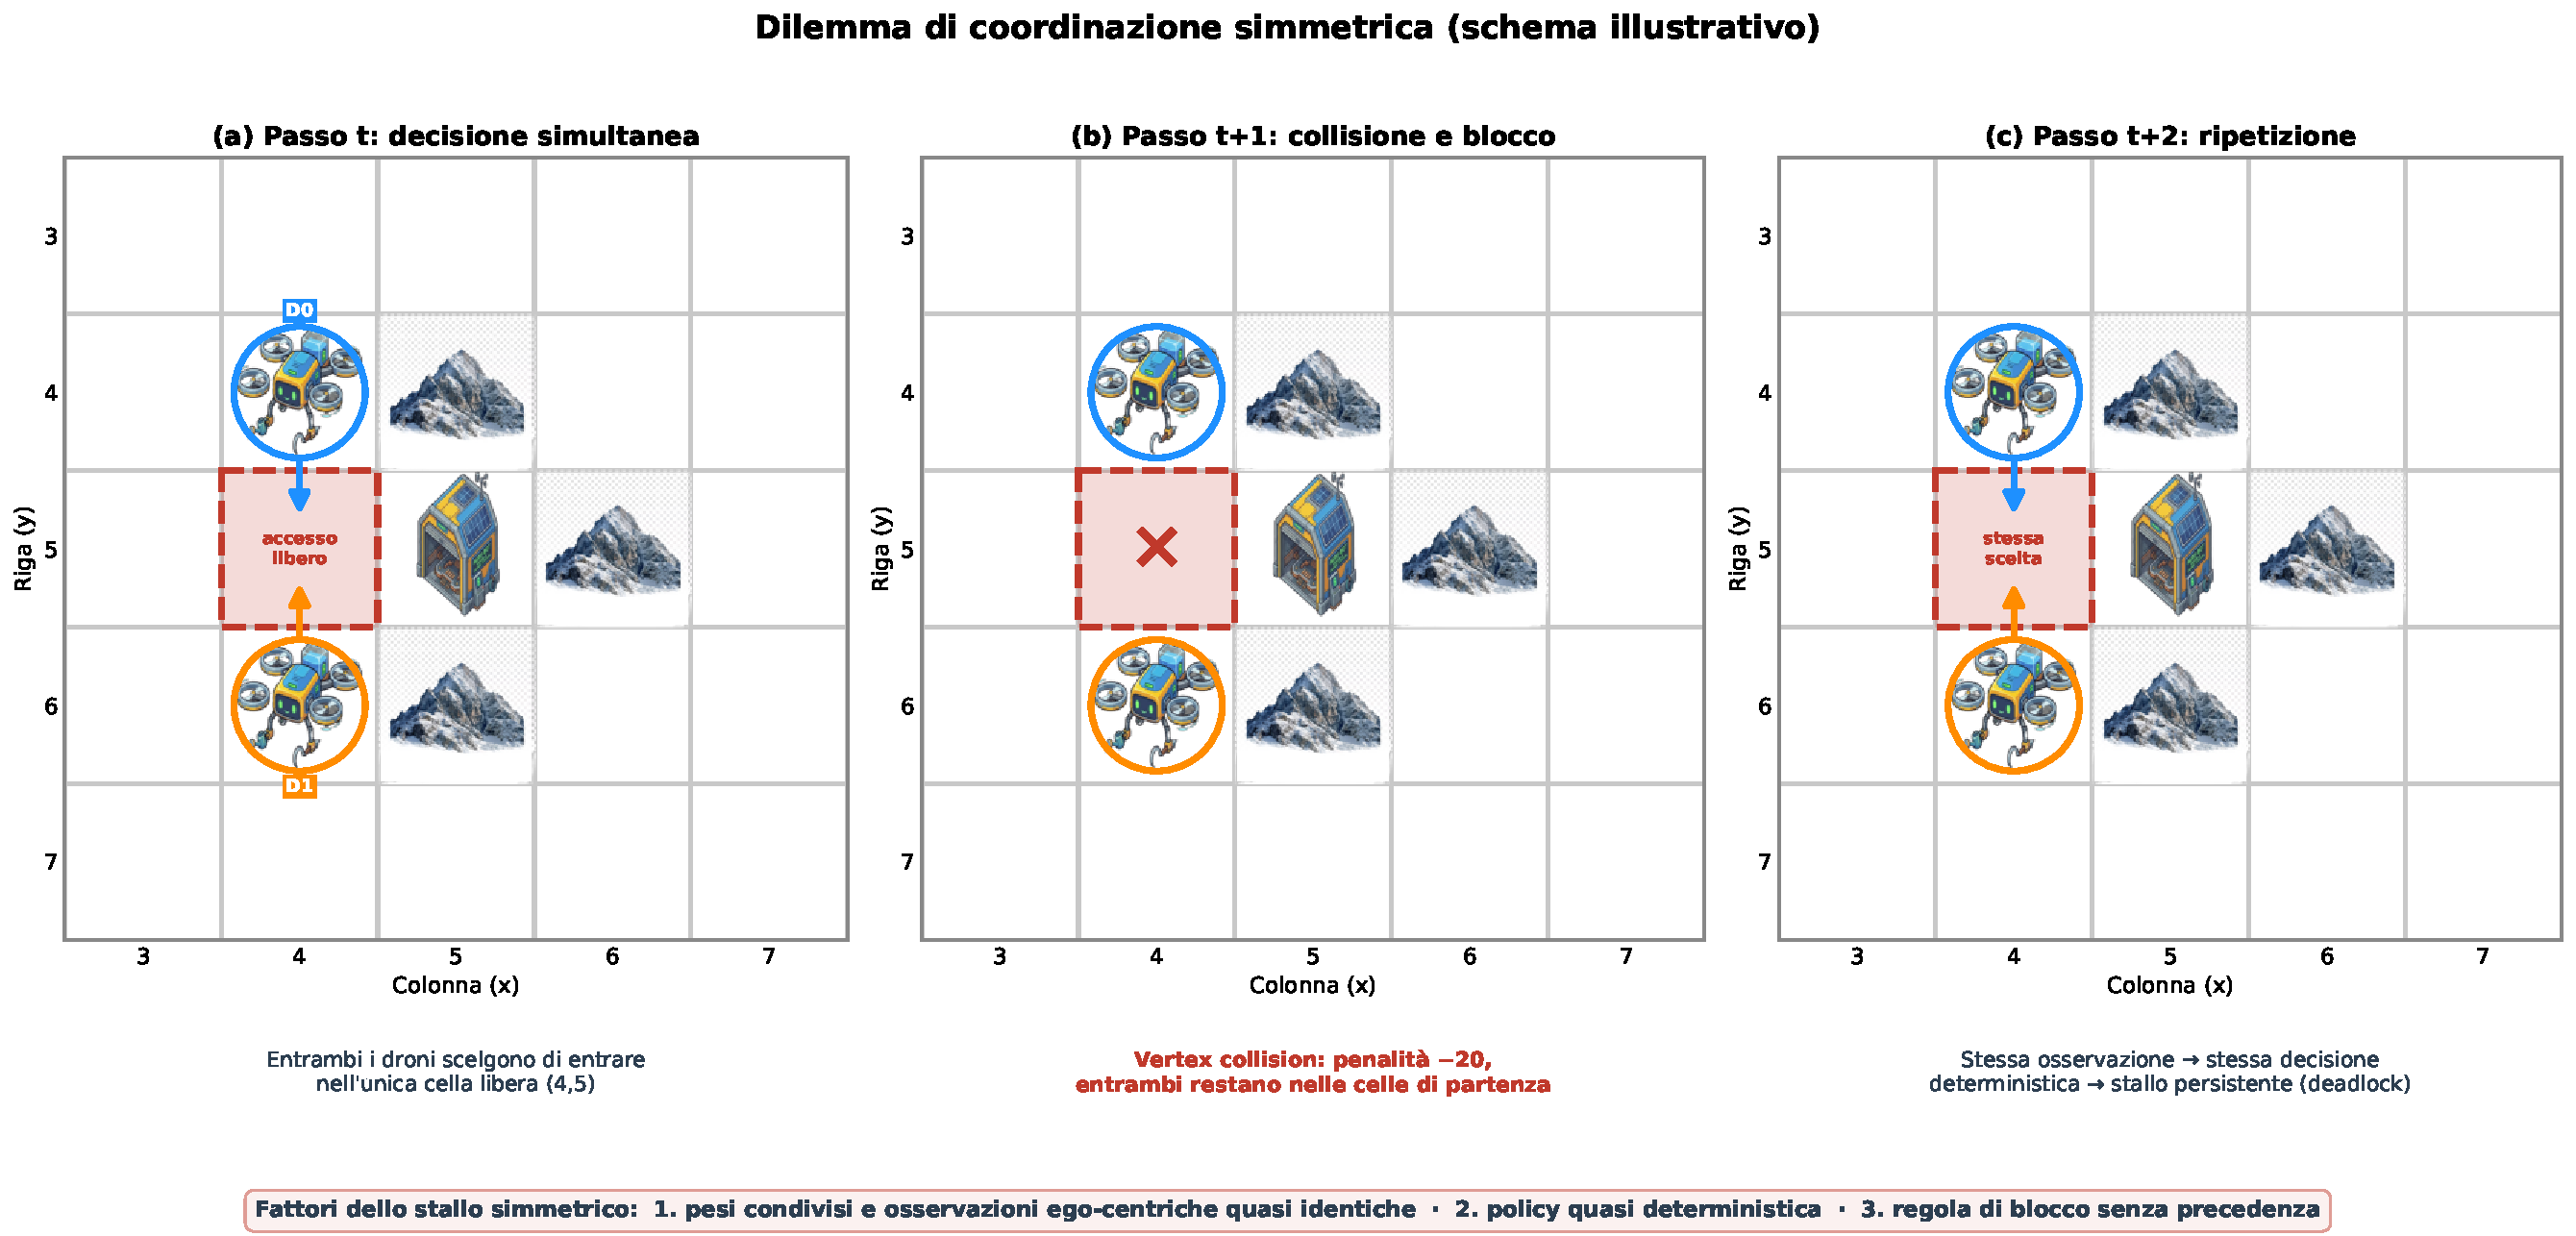
\includegraphics[width=0.95\textwidth]{fig_7_7_dilemma_simmetrico.pdf}
    \caption{Dilemma di coordinazione simmetrica (schema illustrativo, non uno degli scenari testati): due droni in posizioni speculari rispetto all'unico accesso libero all'hangar scelgono la stessa cella, vengono bloccati e ripetono la stessa decisione.}
    \label{fig:7_7}
\end{figure}

\section{Anatomia degli stalli}
\label{sec:anatomia_stalli}

L'osservazione diretta degli episodi falliti e un test su $300$ episodi per algoritmo ($100$ per seme, policy deterministica, ambiente standard) hanno permesso di individuare due configurazioni ricorrenti di stallo (Figura~\ref{fig:7_8}).
\begin{itemize}
    \item \textbf{Caso 1 -- Contesa ai lati dell'hangar.} Lo stallo non avviene sull'hangar: due droni che vi entrano nello stesso passo da lati diversi atterrano entrambi, perché l'hangar è escluso dalla vertex collision. Avviene invece un passo prima, quando due droni tentano di raggiungere la stessa cella adiacente all'hangar. La collisione li riporta alle posizioni precedenti, la configurazione si ripete e lo stallo può durare per decine di passi.
    \item \textbf{Caso 2 -- Varco di una cella tra montagna e bordo.} Quando una montagna lascia un solo corridoio di una cella verso il bordo della mappa e due o più droni devono attraversarlo, oppure quando l'azione più probabile di un drone punta contro la montagna stessa, i droni restano bloccati.
\end{itemize}

\begin{figure}[htbp]
    \centering
    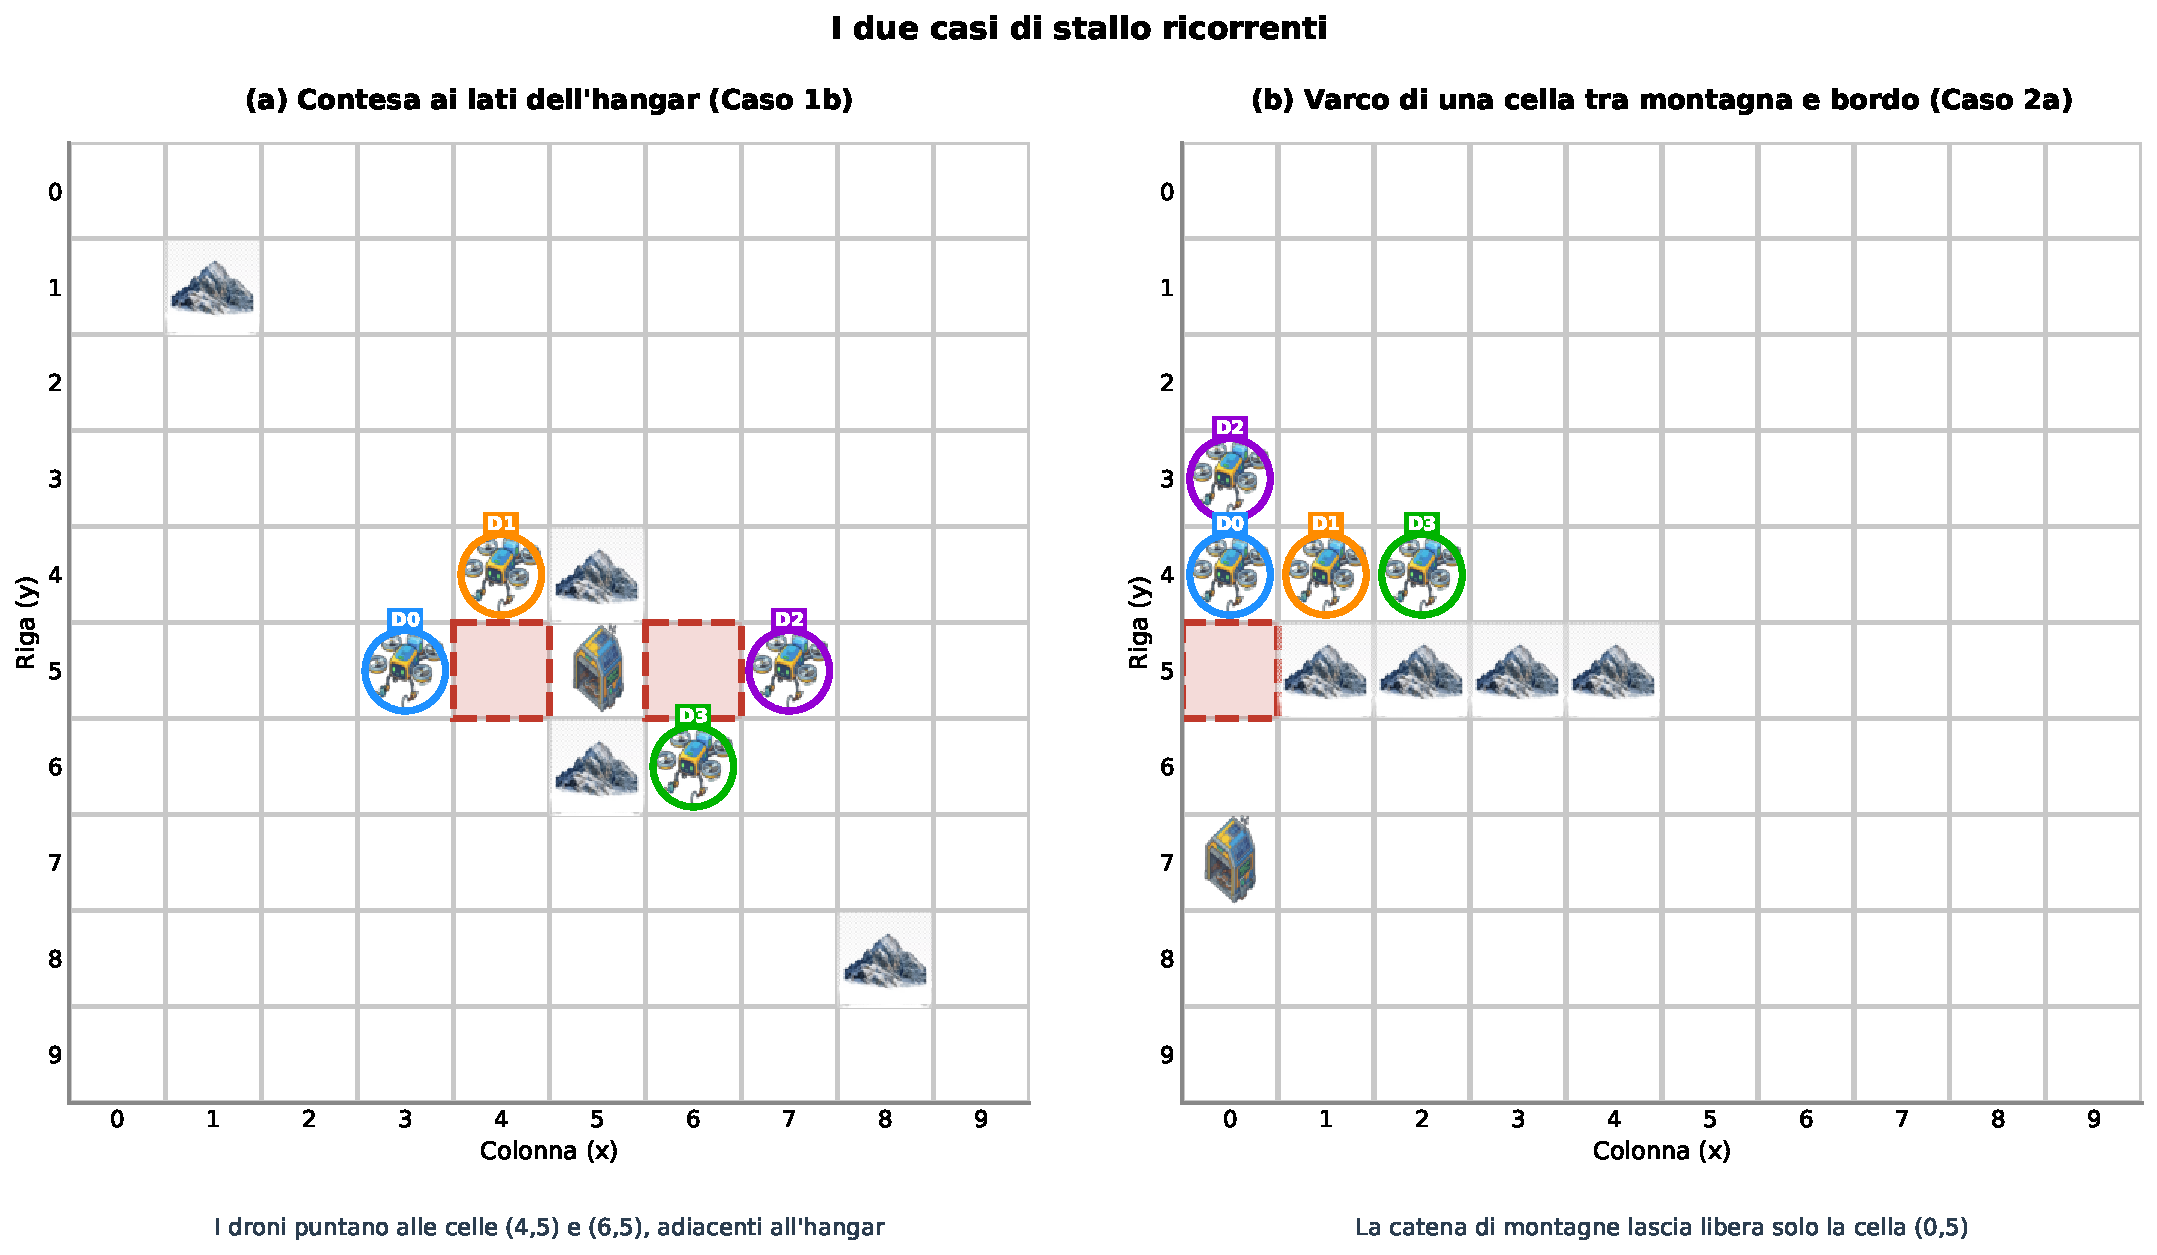
\includegraphics[width=0.95\textwidth]{fig_7_8_tipi_stallo.pdf}
    \caption{I due casi di stallo ricorrenti: (a) contesa ai lati dell'hangar (Caso 1b); (b) varco di una cella tra montagna e bordo (Caso 2a).}
    \label{fig:7_8}
\end{figure}

La Tabella~\ref{tab:7_3} riporta la frequenza dei fallimenti e delle loro cause nell'ambiente standard.

\begin{table}[htbp]
    \centering
    \begin{tabular}{lcc}
        \toprule
        \textbf{Metrica (300 episodi, ambiente standard)} & \textbf{MAPPO} & \textbf{PPO centralizzato} \\
        \midrule
        Episodi completati                              & $64$ ($21,3\%$)  & $141$ ($47,0\%$) \\
        Episodi falliti                                 & $236$ ($78,7\%$) & $159$ ($53,0\%$) \\
        Vertex collision totali                         & $7.444$          & $6.002$ \\
        Droni non arrivati (media per episodio fallito) & $567$ ($2,40$)   & $305$ ($1,92$) \\
        -- rimasti bloccati nella stessa cella          & $450$ ($79,4\%$) & $265$ ($86,9\%$) \\
        -- in movimento continuo senza progredire       & $117$ ($20,6\%$) & $40$ ($13,1\%$) \\
        Caso 1 almeno una volta / fino a fine episodio  & $12,7\%$ / $9,3\%$  & $10,1\%$ / $9,4\%$ \\
        Caso 2 almeno una volta / fino a fine episodio  & $17,8\%$ / $12,3\%$ & $23,9\%$ / $23,3\%$ \\
        \bottomrule
    \end{tabular}
    \caption{Frequenza e cause dei fallimenti a quattro droni nell'ambiente standard (percentuali dei casi riferite agli episodi falliti).}
    \label{tab:7_3}
\end{table}

Gli stalli (deadlock) prevalgono nettamente sulle oscillazioni (livelock). I due casi catalogati spiegano solo una parte dei fallimenti: riguardano circa il $22\%$ degli episodi falliti di MAPPO e il $33\%$ di quelli di PPO. La quota restante è attribuibile ad altre configurazioni di blocco, in particolare ai droni fermi contro un ostacolo, coerentemente con la scomposizione della ricompensa. Il Caso 2 è più frequente per PPO, il Caso 1 è di entità simile nei due algoritmi. I tassi di successo di questo test ($21,3\%$ e $47,0\%$) differiscono da quelli della Tabella~\ref{tab:7_1} perché la sequenza di episodi è diversa.

\section{Soluzioni considerate}
\label{sec:soluzioni_considerate}

Prima di intervenire sul codice sono state valutate tre possibili modifiche alla meccanica di risoluzione dei conflitti.
\begin{itemize}
    \item \textbf{Soluzione A -- Rottura della simmetria con regola di precedenza.} Invece di bloccare entrambi i droni che contendono la stessa cella, si assegna la precedenza a uno dei due (quello che si avvicina all'hangar e, a parità, quello con indice minore), mentre l'altro attende un passo.
    \item \textbf{Soluzione B -- Area di atterraggio estesa.} Si considera atterrato un drone non appena raggiunge una delle celle adiacenti all'hangar.
    \item \textbf{Soluzione C -- Disimpegno casuale.} In caso di collisione si applica una deviazione casuale al movimento dei droni coinvolti.
\end{itemize}

È stata scelta ed estesa la Soluzione A, combinata con il mascheramento delle azioni non valide e con un meccanismo anti-livelock, applicati in fase di esecuzione senza riaddestramento. Questa scelta lascia invariata la definizione del compito, poiché l'hangar resta una singola cella su cui devono convergere tutti i droni. Infine, non richiede di ripetere gli addestramenti, che a $4.000.000$ di passi richiedono circa $1$ ora e mezza per run di MAPPO.

% =============================================================================
% CAPITOLO 8 - STRATO DI RISOLUZIONE DEI CONFLITTI
% =============================================================================
\chapter{Strato di risoluzione dei conflitti}
\label{chap:strato_risoluzione}

Il capitolo descrive lo strato introdotto in fase di esecuzione per eliminare gli stalli individuati e ne riporta la validazione su scenari critici e su un test di $300$ episodi per algoritmo.

\section{Principio e posizionamento}
\label{sec:principio_posizionamento}

Lo strato di risoluzione dei conflitti si colloca tra le policy addestrate e l'ambiente, ed è applicato in esecuzione ai modelli già addestrati a quattro droni con $4.000.000$ di passi (MAPPO e PPO), senza alcun riaddestramento. È composto da tre meccanismi:
\begin{itemize}
    \item una regola di precedenza, che risolve nell'ambiente le contese di più droni sulla stessa cella libera;
    \item un mascheramento delle azioni non valide (action masking), che agisce sulla selezione dell'azione a partire dai logit della rete;
    \item un meccanismo anti-livelock, che interrompe le oscillazioni cicliche.
\end{itemize}

Lo strato è una componente distinta dalle policy, e i requisiti informativi dei tre meccanismi sono diversi. Il mascheramento e il meccanismo anti-livelock usano solo informazioni di cui ogni drone dispone individualmente: la propria posizione, quella degli ostacoli, la propria traiettoria recente e l'esito del proprio ultimo movimento. La regola di precedenza, invece, richiede di conoscere le mosse che i droni intendono compiere nello stesso passo, e presuppone quindi un arbitro centrale o una comunicazione tra i droni. Il sistema risultante non è più a esecuzione puramente decentralizzata, e i risultati di questo capitolo vanno letti come prestazioni dell'insieme di policy e strato, non della sola policy. Nei test i tre meccanismi sono sempre attivati insieme: il contributo di ciascuno non è stato misurato separatamente. La Figura~\ref{fig:8_1} schematizza il funzionamento dello strato.

\begin{figure}[htbp]
    \centering
    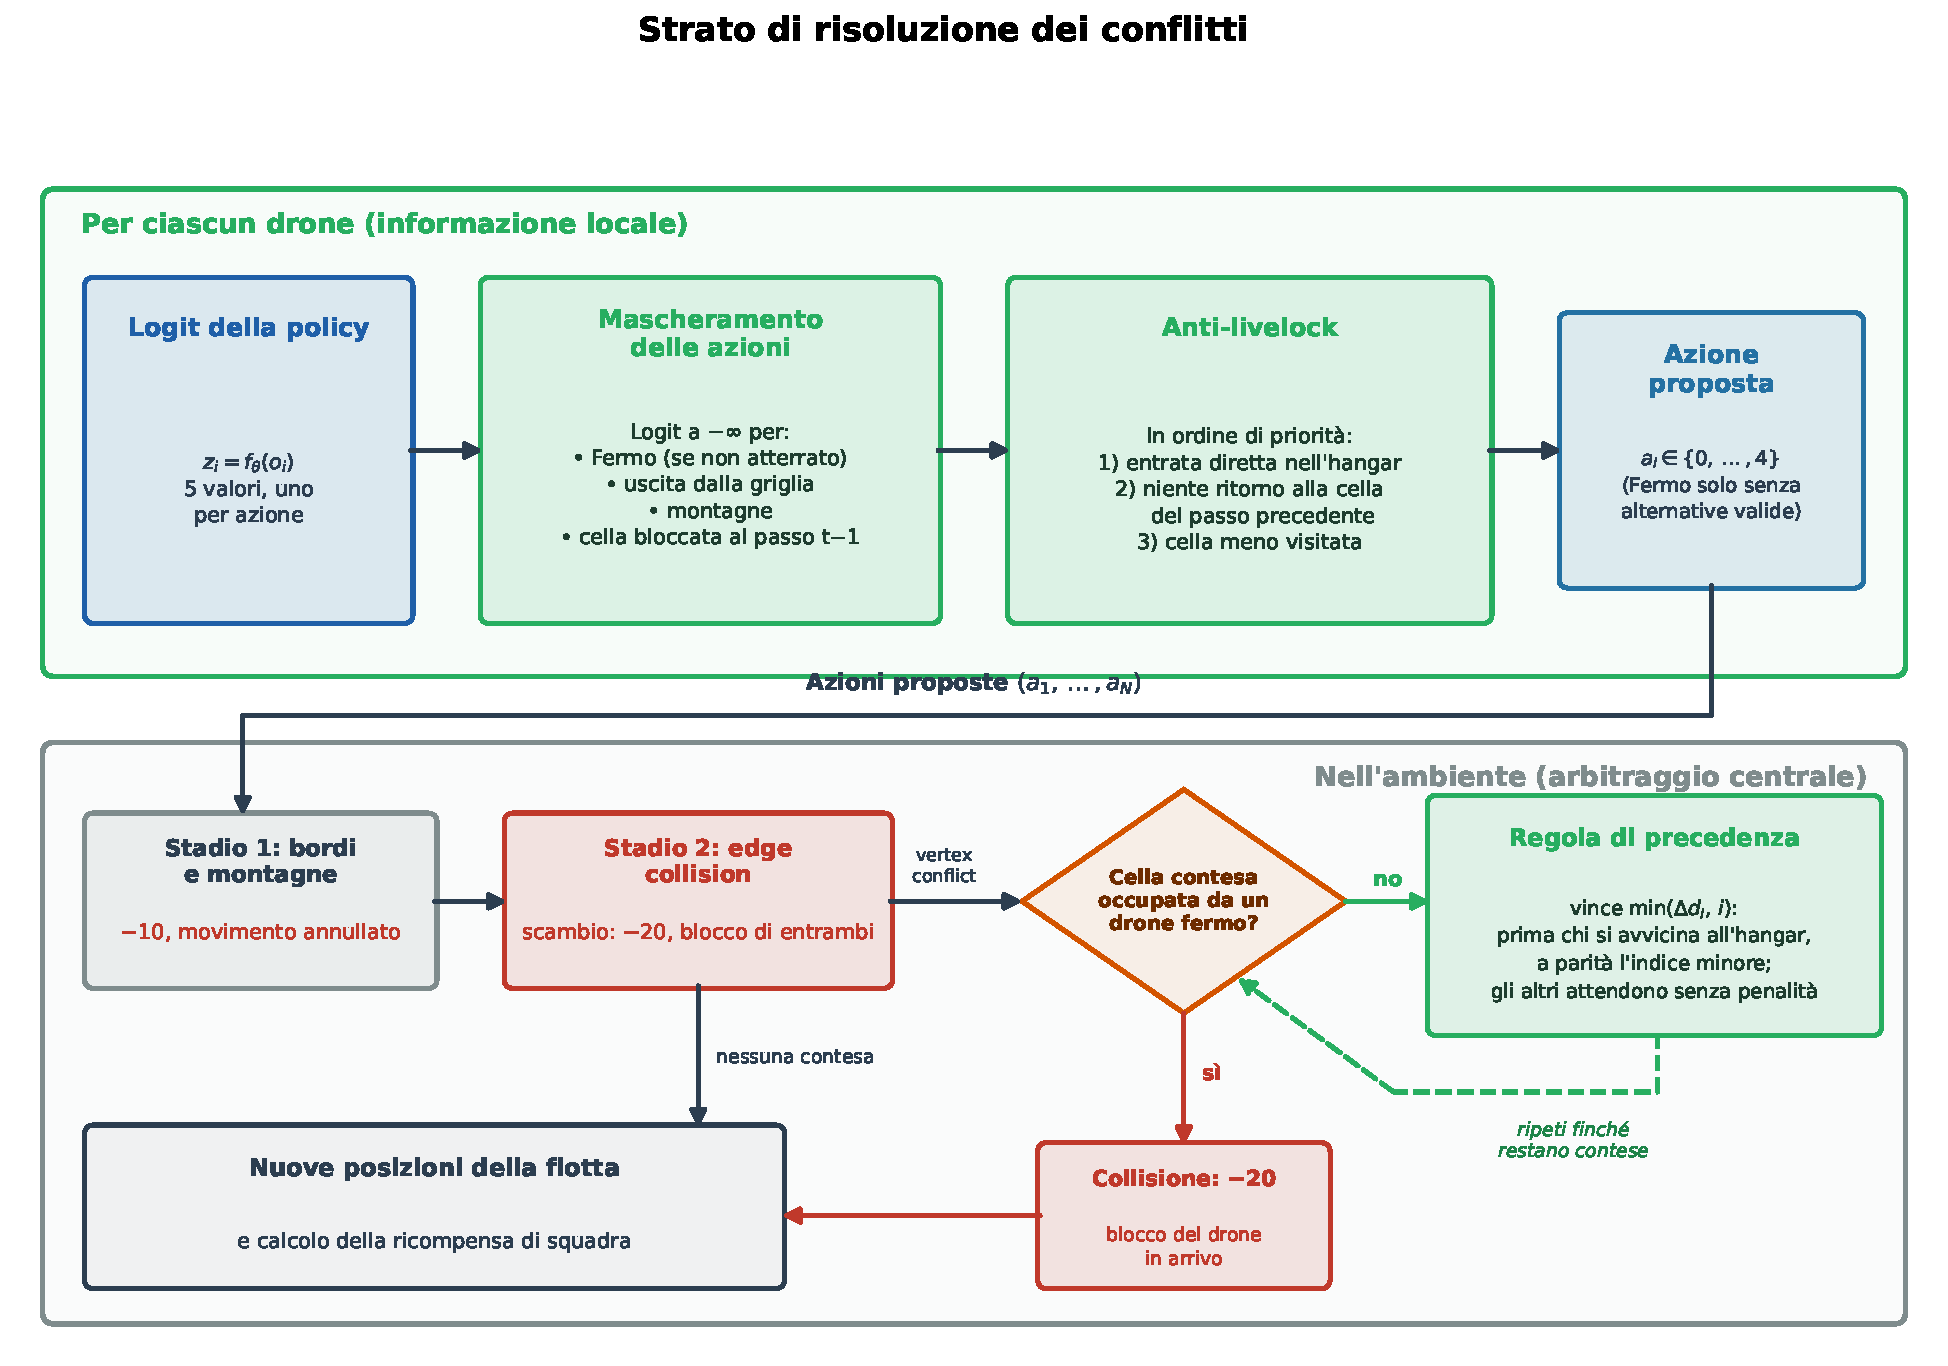
\includegraphics[width=0.95\textwidth]{fig_8_1_strato_risoluzione.pdf}
    \caption{Strato di risoluzione dei conflitti: mascheramento e anti-livelock applicati da ciascun drone ai logit della policy, poi i due stadi dell'ambiente con la regola di precedenza.}
    \label{fig:8_1}
\end{figure}

\section{Regola di precedenza}
\label{sec:regola_precedenza}

La regola modifica il secondo stadio del metodo \texttt{step()}. Il primo stadio, con l'annullamento dei movimenti verso bordi e ostacoli e la relativa penalità, resta invariato, così come il trattamento delle edge collision, che continuano a essere penalizzate e bloccate. I vertex conflict sono invece risolti in modo iterativo:
\begin{itemize}
    \item se la cella contesa è già occupata da un drone che vi rimane, gli altri droni che tentano di entrarvi sono bloccati e la collisione è penalizzata come nell'ambiente standard;
    \item se la cella contesa è libera, passa un solo drone e gli altri attendono nella propria cella per un passo, senza penalità.
\end{itemize}

Il vincitore è il drone che minimizza la coppia $(\Delta d_i, i)$, dove $\Delta d_i = d(c, h) - d(p_i, h)$ è la variazione della distanza di Manhattan dall'hangar $h$ che il drone $i$ otterrebbe entrando nella cella contesa $c$: ha la precedenza il drone che si avvicina all'hangar ($\Delta d = -1$) rispetto a quello che se ne allontana ($\Delta d = +1$) e, a parità, il drone con indice minore. Poiché un drone che attende può a sua volta liberare o occupare celle contese da altri, la procedura viene ripetuta finché non restano contese, gestendo così i blocchi a cascata. L'hangar resta escluso dalle contese.

\section{Mascheramento delle azioni non valide}
\label{sec:mascheramento}

Nel test dell'ambiente standard il $79,4\%$ dei droni non arrivati di MAPPO ($450$ su $567$) e l'$86,9\%$ di quelli di PPO ($265$ su $305$) rimane fermo nella stessa cella fino al termine dell'episodio. La causa è la selezione deterministica: quando l'azione più probabile punta fuori dalla griglia, contro una montagna o coincide con l'azione Fermo, il drone la ripete a ogni passo. Nel Caso 2b, ad esempio, i quattro droni di MAPPO scelgono Fermo per tutti i $100$ passi, ottenendo esattamente il reward di riferimento di $-400$.

Il mascheramento interviene prima della selezione. Dalla rete si estraggono i cinque logit di ciascun drone e si pone a $-\infty$ il logit delle azioni:
\begin{itemize}
    \item Fermo, finché il drone non ha raggiunto l'hangar;
    \item che porterebbero fuori dalla griglia o dentro una montagna;
    \item che porterebbero verso una cella nella quale il drone è stato bloccato da un altro drone al passo precedente, purché esistano alternative valide.
\end{itemize}
Viene quindi scelta l'azione con il logit più alto tra quelle rimaste, cioè la migliore alternativa valida secondo la policy appresa. Se non resta alcuna azione valida il drone rimane fermo. Escludendo l'azione Fermo, l'attesa di un drone avviene soltanto per effetto della regola di precedenza.

\section{Meccanismo anti-livelock}
\label{sec:anti_livelock}

Il restante $20,6\%$ dei droni non arrivati di MAPPO e il $13,1\%$ di quelli di PPO si muove continuamente senza progredire, tipicamente oscillando tra due celle. Nel Caso 1b, per esempio, il drone D0 di MAPPO raggiunge una cella adiacente all'hangar e poi oscilla per $96$ passi tra le celle $(4, 5)$ e $(4, 4)$, senza mai entrare nel bersaglio. Il meccanismo anti-livelock opera dopo il mascheramento, per ciascun drone, secondo tre regole in ordine di priorità:
\begin{enumerate}
    \item se un'azione valida porta direttamente nell'hangar, viene eseguita;
    \item se l'azione scelta riporterebbe il drone nella cella occupata al passo precedente (ciclo di periodo $2$), si sceglie tra le altre azioni valide quella che porta nella cella meno visitata nell'episodio, a parità di visite quella con il logit più alto;
    \item se il drone sta ripassando su celle già visitate (cella corrente visitata almeno due volte e cella di destinazione almeno una), si preferisce la cella valida meno visitata, per forzare l'aggiramento dell'ostacolo.
\end{enumerate}
Il conteggio delle visite è mantenuto separatamente per ciascun drone nel corso dell'episodio.

\section{Validazione su scenari critici}
\label{sec:validazione_scenari}

Lo strato è stato inizialmente verificato su cinque scenari costruiti manualmente per riprodurre i casi di stallo osservati (Tabella~\ref{tab:8_1}), utilizzando i modelli del seme $42$.

\begin{table}[htbp]
    \centering
    \footnotesize
    \setlength{\tabcolsep}{3.5pt}
    \begin{tabularx}{\textwidth}{l >{\raggedright\arraybackslash}X c l l}
        \toprule
        \textbf{Scenario} & \textbf{Descrizione} & \textbf{Hangar} & \textbf{Montagne} & \textbf{Posizioni iniziali dei droni} \\
        \midrule
        Caso 1a & Due droni già atterrati; D1 e D3 cercano di passare per la stessa cella sopra l'hangar & $(4, 8)$ & $(1, 1), (8, 1), (1, 4), (8, 4)$ & $(4, 8), (5, 7), (4, 8), (4, 6)$ \\
        Caso 1b & Hangar tra due montagne; due droni puntano al lato sinistro e due al lato destro      & $(5, 5)$ & $(5, 4), (5, 6), (1, 1), (8, 8)$ & $(3, 5), (4, 4), (7, 5), (6, 6)$ \\
        Caso 2a & Quattro montagne lasciano libera solo la cella $(0, 5)$ sul bordo sinistro            & $(0, 7)$ & $(1, 5), (2, 5), (3, 5), (4, 5)$ & $(0, 4), (1, 4), (0, 3), (2, 4)$ \\
        Caso 2b & Quattro montagne lasciano libera solo la cella $(5, 0)$ sul bordo superiore           & $(7, 0)$ & $(5, 1), (5, 2), (5, 3), (5, 4)$ & $(4, 0), (4, 1), (3, 0), (4, 2)$ \\
        Caso 2c & Passaggio di una cella lungo il bordo destro                                          & $(9, 8)$ & $(8, 5), (8, 6), (8, 7), (7, 7)$ & $(9, 4), (8, 4), (9, 3), (7, 4)$ \\
        \bottomrule
    \end{tabularx}
    \caption{Scenari critici a quattro droni.}
    \label{tab:8_1}
\end{table}

\begin{table}[htbp]
    \centering
    \resizebox{\textwidth}{!}{%
    \begin{tabular}{llcccccc}
        \toprule
        \textbf{Algoritmo} & \textbf{Scenario} & \textbf{Standard: droni} & \textbf{Con lo strato:} & \textbf{Vertex collision} & \textbf{Precedenze} & \textbf{Mascheramenti} & \textbf{Anti-livelock} \\
         & & \textbf{arrivati (reward)} & \textbf{passi (reward)} & \textbf{(prima $\to$ dopo)} & & & \\
        \midrule
        MAPPO & Caso 1a & 3/4 ($-1$)     & $2$ ($+198$)  & $0 \to 0$   & 0 & 0  & 1  \\
        MAPPO & Caso 1b & 3/4 ($+165$)   & $4$ ($+393$)  & $1 \to 0$   & 1 & 1  & 3  \\
        MAPPO & Caso 2a & 0/4 ($-5.340$) & $12$ ($+374$) & $98 \to 0$  & 0 & 9  & 6  \\
        MAPPO & Caso 2b & 0/4 ($-400$)   & $13$ ($+325$) & $0 \to 1$   & 0 & 39 & 20 \\
        MAPPO & Caso 2c & 2/4 ($-1.967$) & $8$ ($+381$)  & $0 \to 0$   & 1 & 6  & 2  \\
        \midrule
        PPO   & Caso 1a & 2/4 ($-2.200$) & $3$ ($+197$)  & $100 \to 0$ & 1 & 0  & 2  \\
        PPO   & Caso 1b & 3/4 ($-814$)   & $3$ ($+394$)  & $0 \to 0$   & 2 & 3  & 0  \\
        PPO   & Caso 2a & 2/4 ($-2.005$) & $6$ ($+386$)  & $0 \to 0$   & 2 & 4  & 0  \\
        PPO   & Caso 2b & 2/4 ($-2.005$) & $6$ ($+386$)  & $0 \to 0$   & 2 & 4  & 0  \\
        PPO   & Caso 2c & 2/4 ($-1.987$) & $8$ ($+381$)  & $0 \to 0$   & 1 & 3  & 0  \\
        \bottomrule
    \end{tabular}%
    }
    \caption{Esito degli scenari critici senza e con lo strato di risoluzione (modelli del seme 42; fallimento per timeout a 100 passi nel caso standard).}
    \label{tab:8_2}
\end{table}

Nell'ambiente standard tutti e dieci i casi falliscono per timeout; con lo strato tutti si concludono con l'arrivo dei quattro droni, in un numero di passi compreso tra $2$ e $13$. Gli scenari mostrano che stalli apparentemente simili hanno cause diverse. Nel Caso 1a, progettato per riprodurre una contesa, PPO genera $100$ vertex collision, mentre MAPPO non ne genera alcuno e fallisce perché il drone D1 oscilla accanto all'hangar senza entrarvi. Nel Caso 2a MAPPO accumula $98$ scontri e numerosi urti contro le montagne (reward $-5.340$), mentre nel Caso 2b tutti i droni restano fermi. I meccanismi più attivi sono di conseguenza diversi da caso a caso: nei Casi 2a e 2b di MAPPO intervengono soprattutto il mascheramento ($9$ e $39$ volte) e l'anti-livelock ($6$ e $20$), mentre la precedenza interviene al più due volte per scenario.

La traccia del Caso 1b con MAPPO illustra il funzionamento combinato dei tre meccanismi (Figura~\ref{fig:8_2}).
\begin{itemize}
    \item \textbf{Passo 1.} D3 sceglierebbe Sinistra, contro la montagna in $(5, 6)$: il mascheramento la sostituisce con Su. D2 e D3 contendono la cella $(6, 5)$, entrambi a distanza $2$ dall'hangar: per la regola di precedenza passa D2, con indice minore, e D3 attende.
    \item \textbf{Passo 2.} D1, in $(4, 5)$, sceglierebbe Giù, allontanandosi dall'hangar: l'anti-livelock rileva che una mossa valida porta direttamente nel bersaglio e sceglie Destra. D1 e D2 atterrano.
    \item \textbf{Passo 3.} D3 entra nell'hangar per la stessa regola, mentre D0 raggiunge la cella $(4, 5)$.
    \item \textbf{Passo 4.} D0, che nell'ambiente standard da questa cella oscillerebbe verso $(4, 4)$ per $96$ passi, viene indirizzato nell'hangar dall'anti-livelock.
\end{itemize}
L'episodio si conclude in $4$ passi con un reward di $+393$, contro il fallimento per timeout dell'ambiente standard ($3$ droni su $4$ arrivati, reward $+165$).

\begin{figure}[htbp]
    \centering
    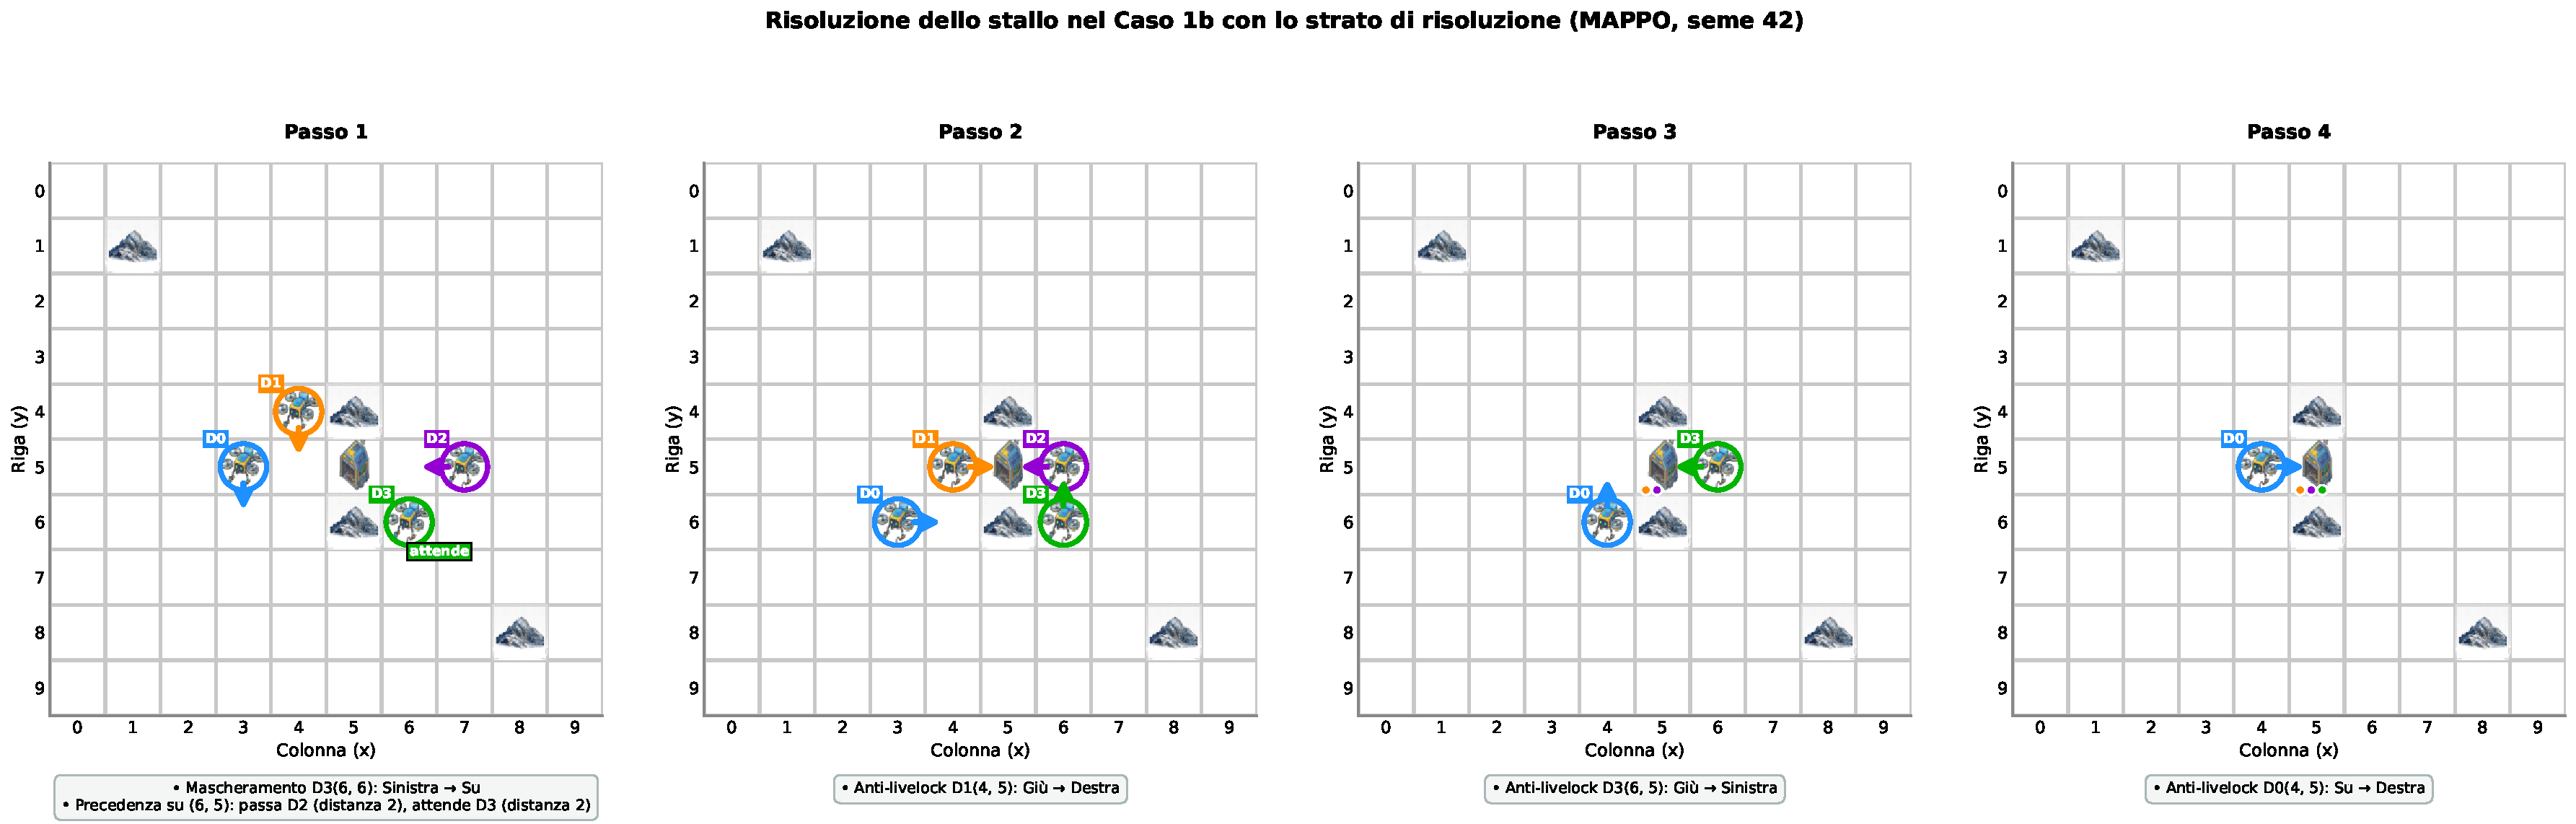
\includegraphics[width=0.95\textwidth]{fig_8_2_traccia_caso_1b.pdf}
    \caption{Traccia del Caso 1b con MAPPO (seme 42): quattro istantanee della griglia (passi 1--4) con le mosse eseguite e le correzioni dello strato.}
    \label{fig:8_2}
\end{figure}

\section{Validazione statistica}
\label{sec:validazione_statistica}

La validazione decisiva è il test su $300$ episodi per algoritmo ($100$ per ciascuno dei semi $42$, $123$ e $999$), con mappe generate, che confronta l'ambiente standard con l'ambiente dotato dello strato (Tabella~\ref{tab:8_3}, Figure~\ref{fig:8_3} e \ref{fig:8_4}).

\begin{table}[htbp]
    \centering
    \resizebox{\textwidth}{!}{%
    \begin{tabular}{lcccc}
        \toprule
        \textbf{Metrica (300 episodi)} & \textbf{MAPPO standard} & \textbf{MAPPO con strato} & \textbf{PPO standard} & \textbf{PPO con strato} \\
        \midrule
        Episodi completati                      & $64$ ($21,3\%$)  & $297$ ($99,0\%$)     & $141$ ($47,0\%$) & $300$ ($100,0\%$) \\
        Vertex collision totali                 & $7.444$          & $2$                  & $6.002$          & $3$ \\
        Interventi della regola di precedenza   & --               & $59$ (in 52 episodi) & --               & $52$ (in 49 episodi) \\
        Interventi del mascheramento            & --               & $3.017$              & --               & $319$ \\
        Interventi anti-livelock                & --               & $1.916$              & --               & $132$ \\
        Contesa ai lati dell'hangar persistente & $22$             & $0$                  & $15$             & $0$ \\
        Varco di una cella persistente          & $29$             & $0$                  & $37$             & $0$ \\
        \bottomrule
    \end{tabular}%
    }
    \caption{Test statistico dello strato di risoluzione dei conflitti a quattro droni (modelli a 4.000.000 di passi).}
    \label{tab:8_3}
\end{table}

\begin{figure}[htbp]
    \centering
    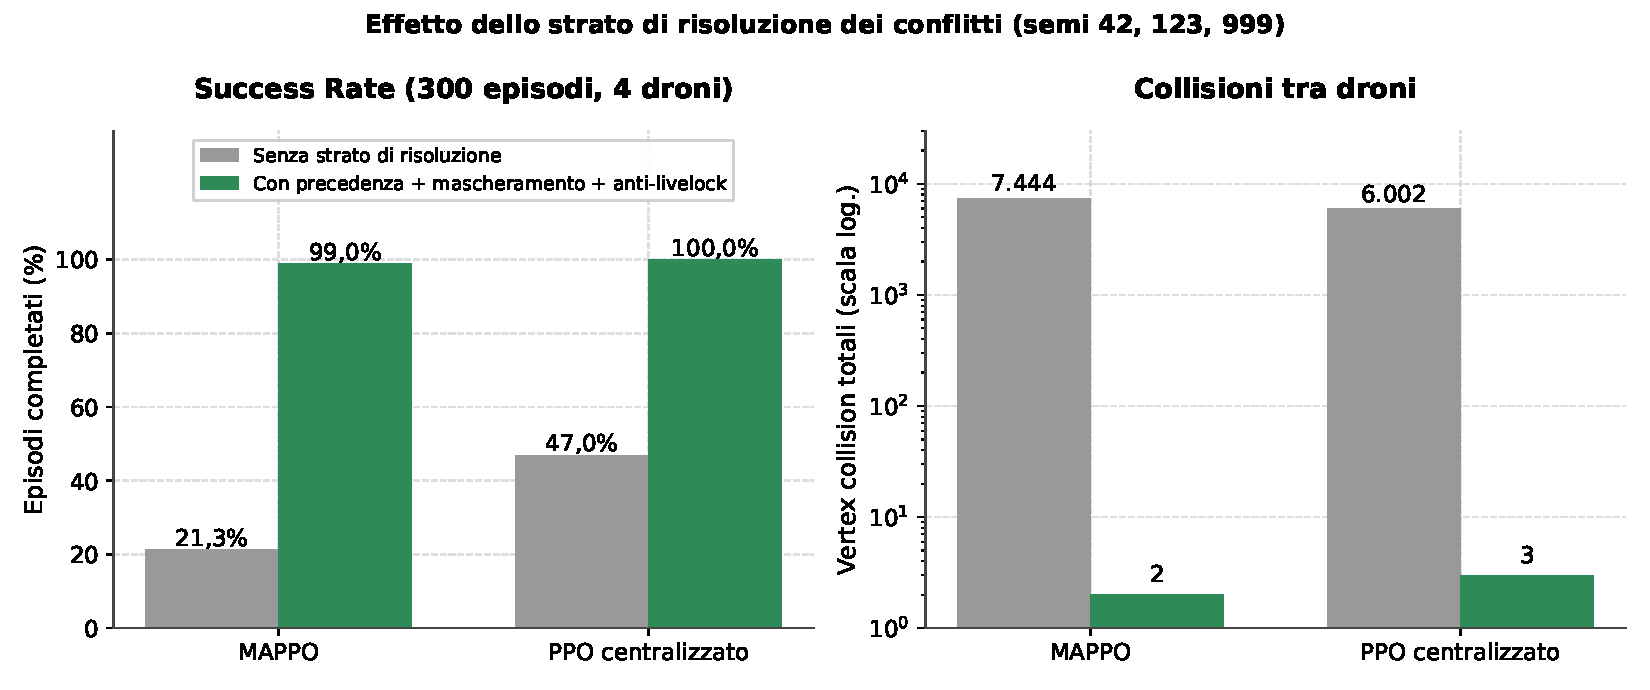
\includegraphics[width=0.95\textwidth]{fig_8_3_strato_sr_collisioni.pdf}
    \caption{Success Rate e vertex collision senza e con lo strato.}
    \label{fig:8_3}
\end{figure}

\begin{figure}[htbp]
    \centering
    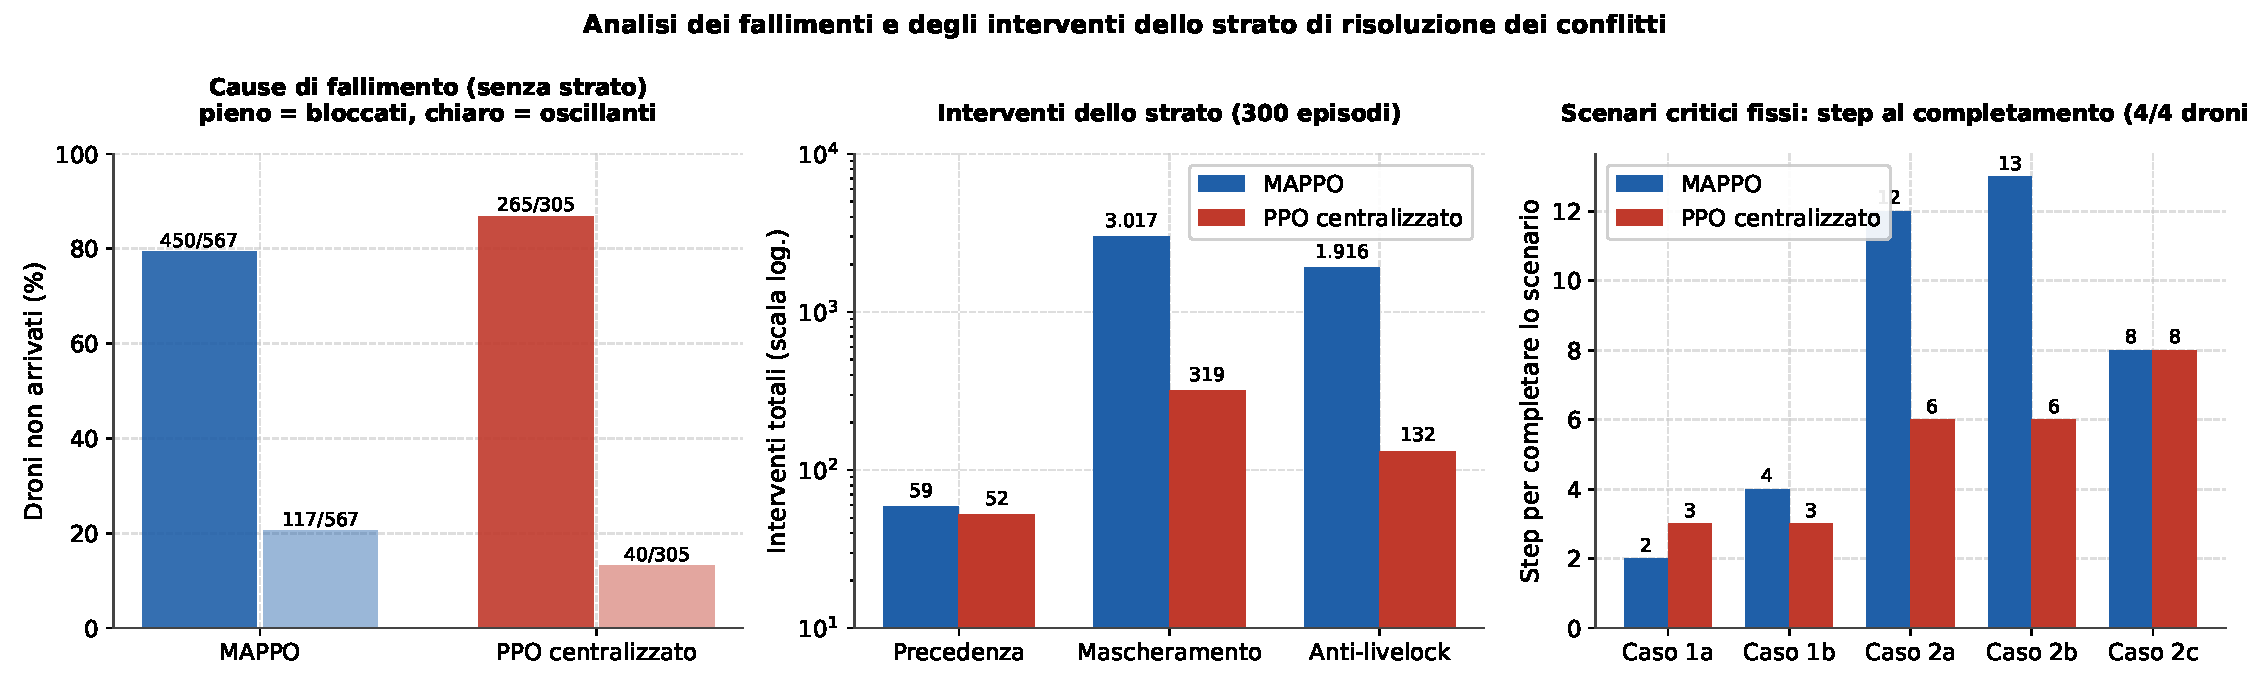
\includegraphics[width=0.95\textwidth]{fig_8_4_strato_cause_interventi.pdf}
    \caption{Cause di fallimento nell'ambiente standard, interventi dello strato e passi di completamento degli scenari critici.}
    \label{fig:8_4}
\end{figure}

Con lo strato il tasso di successo passa dal $21,3\%$ al $99,0\%$ per MAPPO e dal $47,0\%$ al $100,0\%$ per PPO. I tre episodi falliti di MAPPO terminano ciascuno con un solo drone non arrivato, in movimento continuo senza progredire: un livelock residuo che il meccanismo anti-livelock non risolve. Le vertex collision scendono da $7.444$ a $2$ per MAPPO e da $6.002$ a $3$ per PPO. Questa riduzione va interpretata correttamente: nell'ambiente standard gran parte degli scontri si ripete a ogni passo all'interno degli stessi stalli, mentre con lo strato le contese sulle celle libere sono risolte dalla regola di precedenza prima di diventare collisioni e non sono più conteggiate come tali; restano solo i rari casi di un drone che tenta di entrare in una cella occupata da un compagno fermo.

La frequenza degli interventi conferma la diagnosi delle cause di fallimento. Il mascheramento interviene circa dieci volte più spesso per MAPPO ($3.017$ contro $319$) e l'anti-livelock circa quindici volte più spesso ($1.916$ contro $132$): le policy di MAPPO puntano più spesso verso mosse non valide o in ciclo. La regola di precedenza interviene invece raramente e in misura simile per i due algoritmi (in $52$ e $49$ episodi su $300$). I tassi di successo dell'ambiente standard ($21,3\%$ e $47,0\%$) differiscono da quelli del benchmark della Tabella~\ref{tab:7_1} ($18,0\%$ e $41,0\%$) perché la sequenza di episodi è diversa.

\paragraph{Limiti della validazione.} Gli scenari critici sono stati costruiti a mano, il test usa gli stessi semi dell'addestramento e i tre meccanismi sono stati valutati sempre insieme.

% =============================================================================
% CAPITOLO 9 - DISCUSSIONE
% =============================================================================
\chapter{Discussione}
\label{chap:discussione}

Il capitolo interpreta i risultati, li colloca rispetto alla letteratura e discute i limiti del lavoro e le minacce alla validità delle conclusioni.

\section{Interpretazione dei risultati}
\label{sec:interpretazione_risultati}

\paragraph{Scalabilità.} Il tasso di successo di squadra diminuisce rapidamente con il numero di droni per entrambi gli algoritmi, con il calo più marcato tra due e tre droni. Il successo richiede che tutti i droni raggiungano l'hangar, per cui la probabilità di fallimento cresce con il numero di agenti anche a parità di abilità individuale. A ciò si aggiunge la contesa per l'accesso all'unico hangar, che con quattro droni impone un ordine di arrivo.

\paragraph{Confronto tra MAPPO e PPO.} I risultati non indicano una superiorità generale di nessuno dei due approcci. MAPPO è moderatamente avanti con uno e due droni, PPO con tre e quattro; le differenze a $1.000.000$ di passi sono dell'ordine della variabilità tra i semi, mentre a $4.000.000$ di passi il vantaggio di PPO a quattro droni ($41,0\%$ contro $18,0\%$) è netto e concorde in tutti i semi. Con lo strato di risoluzione dei conflitti la distanza si annulla quasi del tutto ($99,0\%$ contro $100,0\%$). Ne segue che a quattro droni gran parte del divario tra i due algoritmi non dipende dalla capacità di navigazione appresa, ma dal modo in cui le policy gestiscono i conflitti in esecuzione.

\paragraph{Addestramento e valutazione.} Il risultato più ricorrente è il divario tra metriche di addestramento, ottenute con policy stocastica, e metriche di valutazione deterministica. La valutazione deterministica, scelta per garantire riproducibilità e confrontabilità, misura quindi una proprietà diversa dalla qualità media della policy stocastica.

\paragraph{Entropia.} L'entropia delle policy di MAPPO cala molto più di quella di PPO, nonostante il bonus di entropia sia presente solo in MAPPO ($0,01$ contro $0,0$). I dati non permettono di isolare la causa, ma suggeriscono alcune ipotesi da verificare: la condivisione dei parametri, per cui l'actor riceve $N$ campioni per passo con il medesimo advantage di squadra; la dimensione maggiore delle reti; il learning rate più elevato del critic, che accelera la stima dell'advantage.

\paragraph{Strato di risoluzione dei conflitti.} Uno strato semplice, composto da regole deterministiche e senza riaddestramento, porta il successo vicino al $100\%$. Le policy apprese contengono quindi già una buona capacità di navigazione, e ciò che manca è soprattutto la capacità di risolvere le situazioni di stallo. Questo suggerisce una divisione dei compiti tra apprendimento e regole: le policy si occupano della navigazione verso l'obiettivo, mentre la sicurezza e la precedenza sono affidate a uno strato esplicito, verificabile e prevedibile.

\section{Confronto con la letteratura}
\label{sec:confronto_letteratura}

MAPPO ha ottenuto prestazioni competitive su numerosi benchmark cooperativi \parencite{yu2022}. I risultati di questa tesi non contraddicono quel lavoro, ma evidenziano un limite in un contesto specifico: agenti omogenei con osservazioni ego-centriche e parametri condivisi, valutati in modo deterministico, in un compito con una risorsa unica contesa. In letteratura è noto che la condivisione completa dei parametri può limitare la diversificazione dei comportamenti tra agenti \parencite{christianos2021}. Una pratica diffusa per attenuare il problema è aggiungere all'osservazione un identificativo dell'agente, che consente alla rete condivisa di specializzare il comportamento di ciascun drone e di rompere la simmetria; nelle osservazioni di questa tesi tale identificativo è assente.

La regola di precedenza riprende un'idea consolidata nella pianificazione multi-agente, la pianificazione prioritaria \parencite{silver2005}, e lo strato nel suo complesso è affine ai meccanismi di sicurezza che filtrano le azioni di una policy appresa prima dell'esecuzione.

\section{Limiti del lavoro e scelte di compromesso}
\label{sec:limiti_lavoro}

\subsection*{Validità interna.}
\begin{itemize}
    \item \textbf{Configurazioni non controllate.} MAPPO e PPO differiscono anche negli iperparametri e nell'implementazione. L'implementazione di MAPPO, inoltre, non include la normalizzazione della value function, che potrebbero migliorarne le prestazioni. Le differenze osservate non sono attribuibili al solo paradigma CTDE o al parameter sharing.
    \item \textbf{Budget comune.} I budget del confronto principale sono un compromesso tra i due algoritmi. Un confronto con budget ottimizzato per ciascun algoritmo, o con selezione del modello migliore durante l'addestramento, potrebbe dare risultati diversi.
    \item \textbf{Assenza di ablazione.} I tre meccanismi dello strato sono stati valutati sempre insieme, per cui il contributo di ciascuno non è quantificato.
\end{itemize}

\subsection*{Validità statistica.}
\begin{itemize}
    \item \textbf{Numero di semi.} Le conclusioni si basano su tre semi. Le deviazioni standard misurano la dispersione tra tre modelli e sono quindi stime poco precise; a $1.000.000$ di passi le differenze tra gli algoritmi non risultano significative con questo campione.
    \item \textbf{Sequenze di episodi diverse.} Benchmark, analisi della ricompensa e test dello strato usano sequenze di episodi diverse, per cui i tassi di successo dell'ambiente standard variano tra le analisi (ad esempio $18,0\%$, $16,7\%$ e $21,3\%$ per MAPPO a quattro droni). Le variazioni sono coerenti con l'errore campionario, ma impongono di confrontare i valori solo all'interno della stessa analisi.
\end{itemize}

\subsection*{Validità di costrutto.}
\begin{itemize}
    \item \textbf{Metriche.} Il reward medio è dominato dagli episodi falliti e i passi medi includono gli episodi troncati: entrambe le metriche vanno lette insieme al tasso di successo.
    \item \textbf{Conteggio delle collisioni.} Con lo strato le contese risolte dalla precedenza non sono conteggiate come collisioni, per cui la riduzione delle vertex collision è in parte una conseguenza della definizione.
    \item \textbf{Valutazione deterministica.} Esaminare la policy deterministica mira a misurare una proprietà ben definita della flotta: condurre invece una valutazione stocastica fornirebbe riscontri diversi e plausibilmente più coerenti con le metriche di addestramento.
\end{itemize}

\subsection*{Validità esterna.}
\begin{itemize}
    \item \textbf{Astrazione.} L'ambiente è una griglia discreta $10 \times 10$, senza dinamica continua, quota, vento, rumore di sensori né vincoli di comunicazione. I risultati non sono direttamente trasferibili al volo reale.
    \item \textbf{Configurazione del problema.} Le flotte arrivano a quattro droni, gli ostacoli sono statici e la destinazione è unica e comune. Non è verificato come le conclusioni si estendano a flotte più numerose o a destinazioni multiple.
    \item \textbf{Generalizzazione.} I test usano gli stessi semi dell'addestramento, con sequenze di mappe nuove ma generate dallo stesso processo. Non è misurata la generalizzazione a semi non visti né a mappe con distribuzione diversa.
    \item \textbf{Scenari critici.} I cinque scenari sono stati costruiti dopo aver osservato i fallimenti e non costituiscono un campione rappresentativo.
    \item \textbf{Decentralizzazione.} La regola di precedenza richiede un'arbitrazione centrale o una comunicazione tra i droni, per cui il sistema non è a esecuzione puramente decentralizzata.
\end{itemize}

% =============================================================================
% CAPITOLO 10 - CONCLUSIONI E SVILUPPI FUTURI
% =============================================================================
\chapter{Conclusioni e sviluppi futuri}
\label{chap:conclusioni}

\section{Conclusioni}
\label{sec:conclusioni}

La tesi ha affrontato la navigazione cooperativa di una flotta di UAV verso un hangar comune, su una griglia con ostacoli generati proceduralmente, mediante \emph{Multi-Agent Reinforcement Learning} (MARL). È stato sviluppato un ambiente parametrico compatibile con Gymnasium, con rilevamento delle vertex collision ed edge collision e ricompensa di squadra, formalizzato come processo decisionale di Markov multi-agente a osservabilità completa. Su di esso sono stati confrontati MAPPO, algoritmo esistente \parencite{yu2022} di cui è stata realizzata un'implementazione propria in PyTorch, con parametri condivisi e osservazioni ego-centriche, e un PPO centralizzato basato su Stable-Baselines3, con un protocollo di valutazione su $100$ episodi per ciascuno di tre semi.

I risultati principali sono quattro.
\begin{enumerate}
    \item \textbf{Scalabilità.} Il tasso di successo di squadra diminuisce rapidamente con la dimensione della flotta per entrambi gli algoritmi, dall'$80\%$ circa con un drone al $23$--$26\%$ con quattro droni a $1.000.000$ di passi.
    \item \textbf{Confronto tra gli algoritmi.} MAPPO è moderatamente avanti con uno e due droni e PPO con tre e quattro, con differenze dell'ordine della variabilità tra i semi. Aumentando il budget a $4.000.000$ di passi MAPPO non migliora ($18,0\%$), mentre PPO sale al $41,0\%$.
    \item \textbf{Diagnosi.} Il reward fortemente negativo a quattro droni è dovuto alle collisioni: tra droni, più frequenti per MAPPO, e contro gli ostacoli, più frequenti per PPO. Il degrado di MAPPO è associato a una forte contrazione dell'entropia e a un problema derivante dalle coordinazioni simmetriche, per cui droni con gli stessi pesi in configurazioni equivalenti prendono la stessa decisione e restano bloccati. Le metriche di addestramento stocastiche sono sistematicamente migliori di quelle di valutazione deterministica.
    \item \textbf{Strato di risoluzione dei conflitti.} Uno strato composto da regola di precedenza, mascheramento delle azioni non valide e meccanismo anti-livelock, applicato in esecuzione senza riaddestramento, porta il tasso di successo a quattro droni dal $21,3\%$ al $99,0\%$ per MAPPO e dal $47,0\%$ al $100,0\%$ per PPO, eliminando gli stalli persistenti.
\end{enumerate}

Nel complesso, le policy apprese possiedono una buona capacità di navigazione, mentre la risoluzione dei conflitti tra agenti omogenei in prossimità di una risorsa contesa rimane il punto critico. In questo contesto la combinazione di policy apprese e regole esplicite di coordinamento si è dimostrata più efficace del solo apprendimento, pagando però il prezzo di una regola di precedenza vincolata a un coordinatore centrale.

\section{Sviluppi futuri}
\label{sec:sviluppi_futuri}

I limiti del lavoro suggeriscono diverse linee di sviluppo.
\begin{itemize}
    \item \textbf{Identificativo dell'agente o condivisione selettiva dei parametri.} Aggiungere all'osservazione un identificativo del drone, oppure condividere solo una parte della rete \parencite{christianos2021}, permetterebbe di apprendere comportamenti diversi per ciascun drone e di rompere la simmetria già nella policy, senza ricorrere a uno strato esterno.
    \item \textbf{Rimozione selettiva dei meccanismi dello strato.} Valutare precedenza, mascheramento e anti-livelock singolarmente e in combinazione chiarirebbe il contributo di ciascuno e individuerebbe quelli eventualmente ridondanti.
    \item \textbf{Precedenza decentralizzata.} Sostituire l'arbitrazione centrale con uno scambio di messaggi tra droni vicini, ad esempio la comunicazione della cella che si intende occupare, riporterebbe l'intero sistema a un'esecuzione decentralizzata.
    \item \textbf{Budget ottimizzati e selezione del modello.} Adottare per ciascun algoritmo il proprio budget, oppure valutare il modello al picco di prestazione anziché quello finale, renderebbe il confronto più equo, dato che MAPPO raggiunge il picco molto prima di PPO.
    \item \textbf{Generalizzazione e flotte più numerose.} Valutare i modelli su semi non utilizzati in addestramento misurerebbe la generalizzazione effettiva; estendere gli esperimenti a cinque o più droni verificherebbe la tenuta delle conclusioni sulla scalabilità e sullo strato.
    \item \textbf{Integrazione dello strato nell'addestramento.} Applicare il mascheramento delle azioni non valide già durante l'addestramento \parencite{huang2022} renderebbe coerenti la regola di selezione appresa e quella usata in esecuzione, concentrerebbe l'esplorazione sulle mosse utili e potrebbe ridurre gli interventi correttivi necessari; un confronto tra policy addestrate con e senza maschera, valutate con e senza strato, ne quantificherebbe il beneficio.
    \item \textbf{Ambienti più realistici.} Portare l'approccio in un ambiente continuo o in un simulatore fisico, con dinamica di volo, quota e rumore di misura, è il passo necessario per valutarne la trasferibilità a droni reali.
\end{itemize}

% =============================================================================
% APPENDICE A - TRACCE DEGLI SCENARI CRITICI
% =============================================================================
\appendix
\chapter{Tracce degli scenari critici}
\label{app:tracce}

L'appendice riporta, per ciascuno dei cinque scenari critici del Capitolo~\ref{chap:strato_risoluzione} (Tabella~\ref{tab:8_1}), le tracce passo per passo degli episodi eseguiti con i modelli MAPPO e PPO del seme $42$ addestrati a quattro droni con $4.000.000$ di passi, nell'ambiente standard e con lo strato di risoluzione dei conflitti. Tutti gli episodi sono eseguiti con policy deterministica.

\paragraph{Convenzioni.} Le coordinate sono indicate come $(x, y)$, con $x$ indice di colonna da sinistra a destra e $y$ indice di riga dall'alto verso il basso: l'azione Giù incrementa $y$. Nelle tabelle le posizioni sono quelle all'inizio di ciascun passo, nell'ordine $\text{D0} \cdot \text{D1} \cdot \text{D2} \cdot \text{D3}$, e il simbolo --- indica un drone già atterrato. Le azioni sono quelle effettivamente eseguite, dopo le eventuali correzioni dello strato; la colonna degli eventi riporta urti, collisioni e interventi dello strato, nella forma \guillemotleft{}azione proposta $\to$ azione eseguita\guillemotright{}. I cicli ripetuti fino al termine dell'episodio sono compressi in una sola riga.

\paragraph{Figure.} Ogni figura riporta tre pannelli: (a) la configurazione iniziale, con la cella critica evidenziata dal riquadro tratteggiato rosso; (b) le traiettorie nell'ambiente standard; (c) le traiettorie con lo strato di risoluzione. Le traiettorie sono tracciate nel colore del drone (D0 blu, D1 arancione, D2 viola, D3 verde): un cerchio vuoto indica la posizione iniziale, un marcatore pieno quella finale, la doppia freccia un'oscillazione tra due celle e la croce un drone rimasto fermo.

\begin{figure}[H]
    \centering
    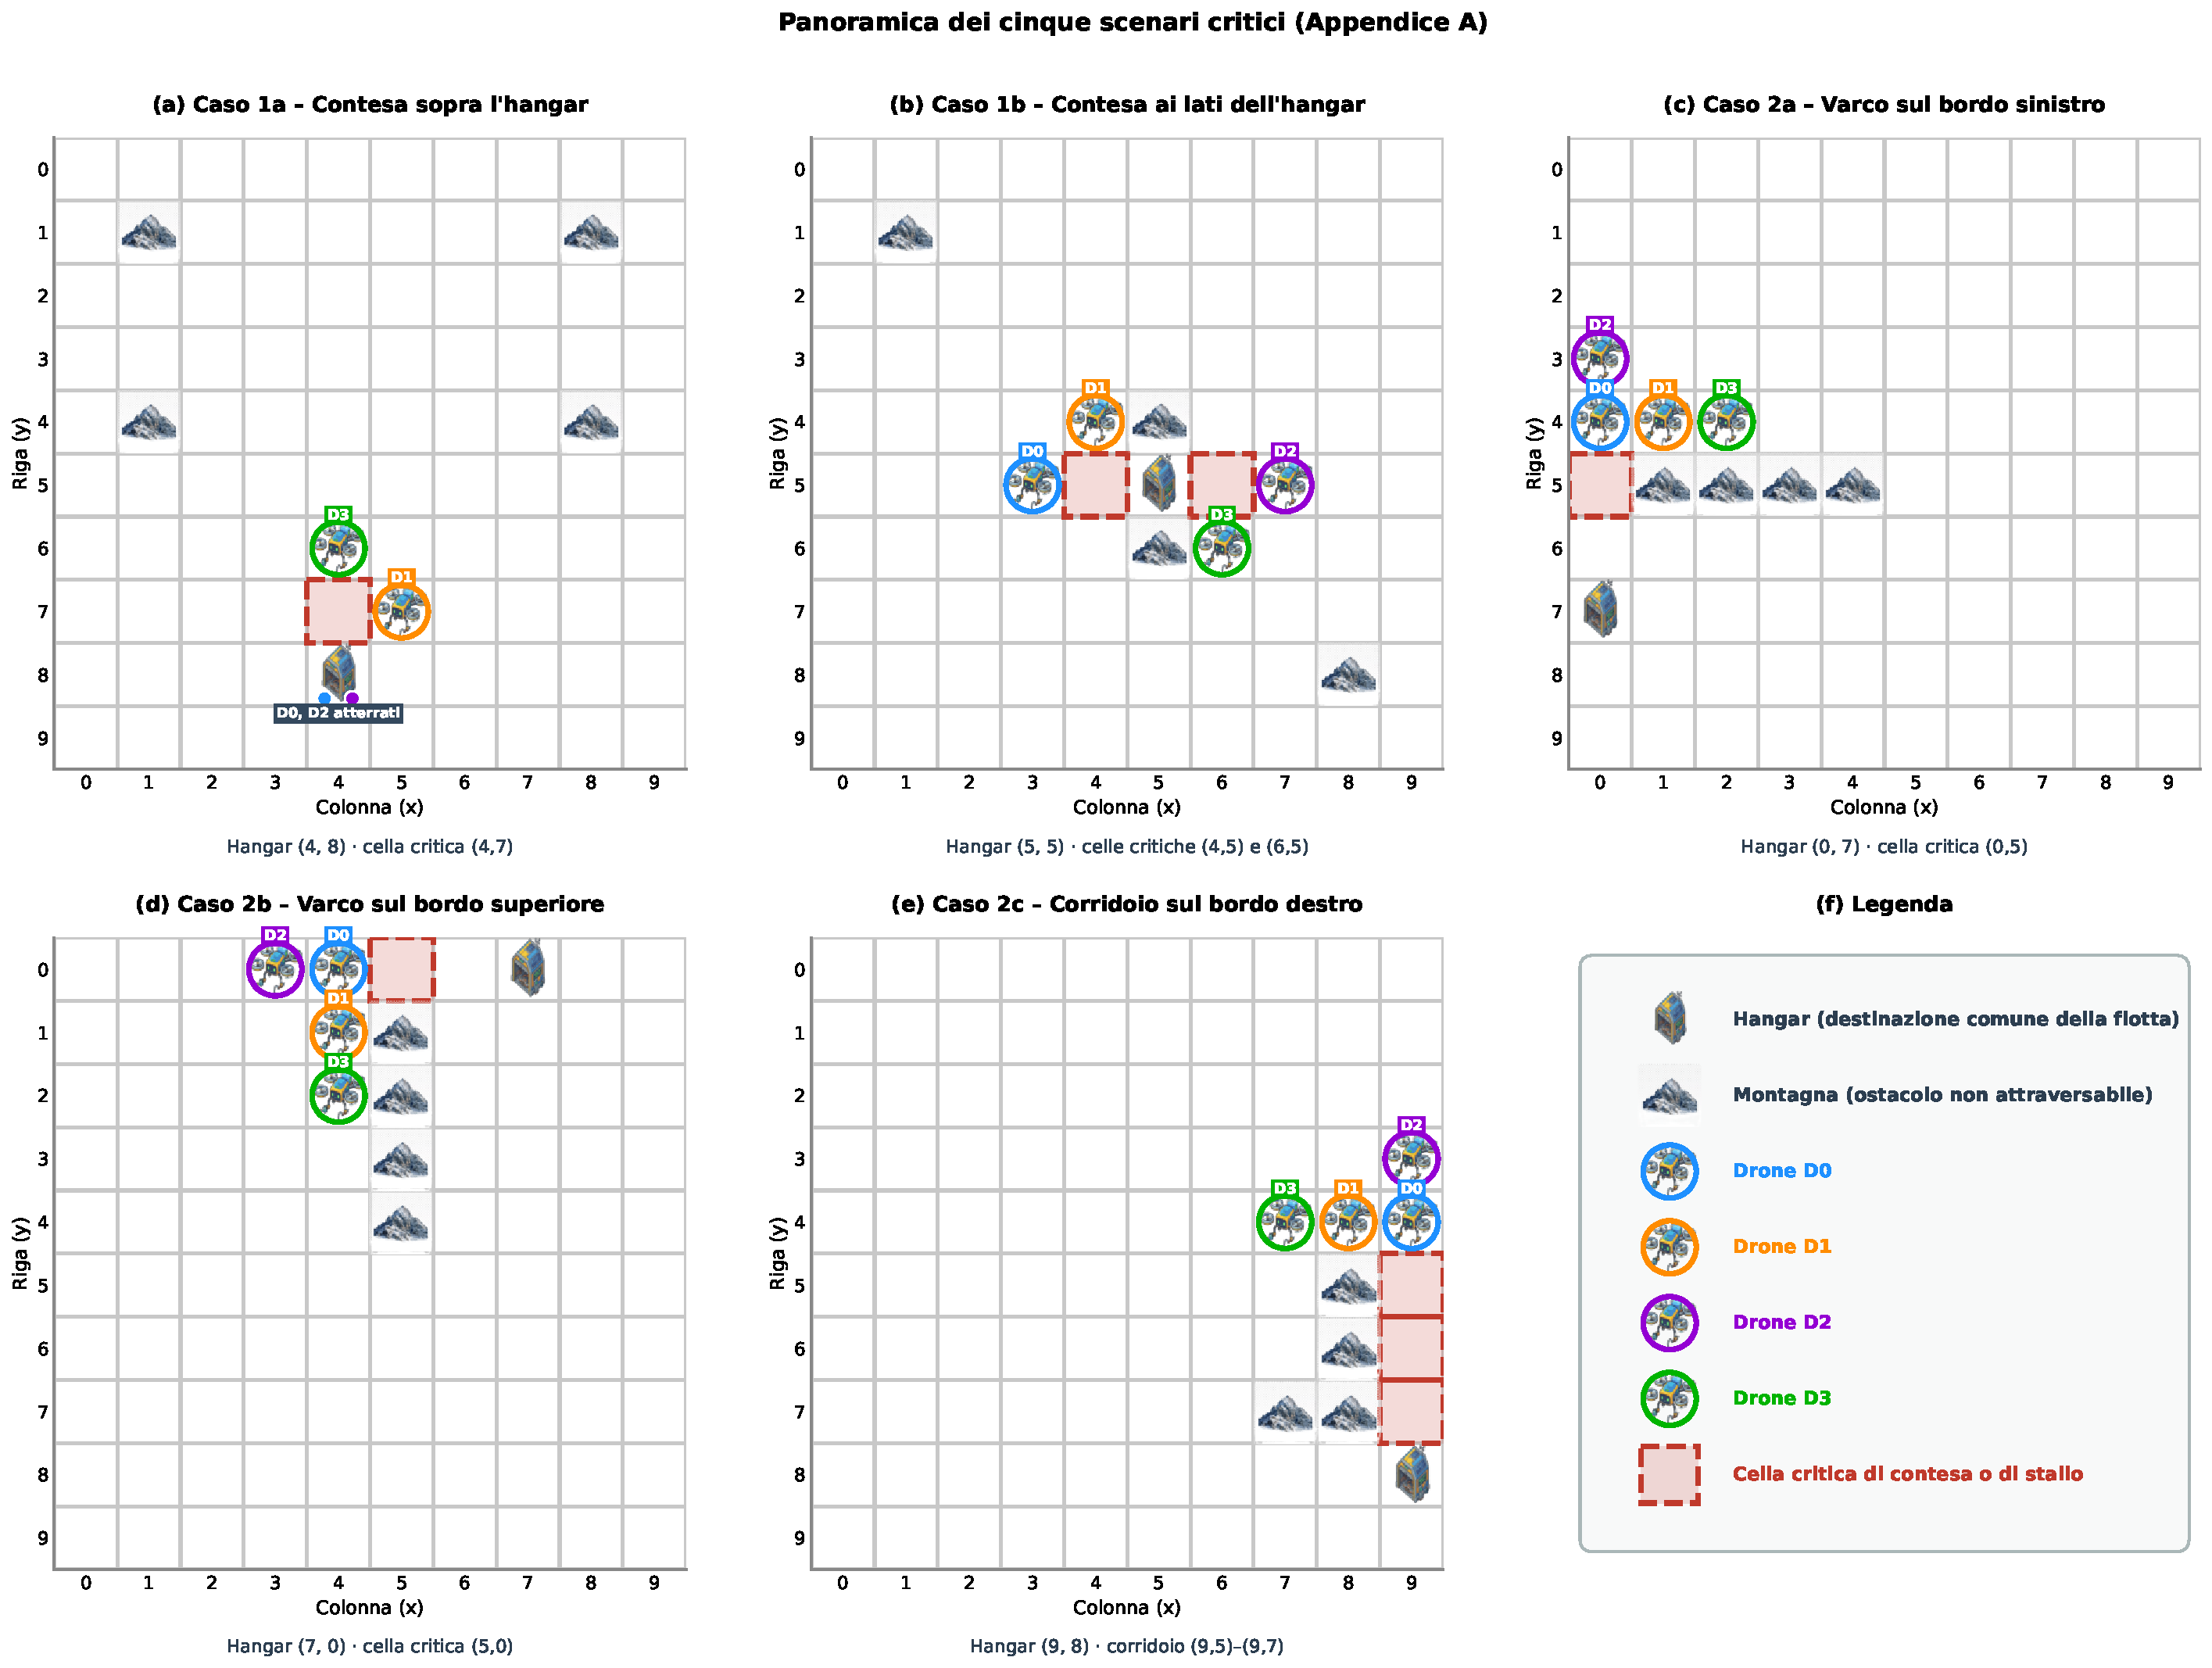
\includegraphics[width=0.98\textwidth]{fig_A_1_panoramica.pdf}
    \caption{Panoramica dei cinque scenari critici e legenda dei simboli.}
    \label{fig:A_1}
\end{figure}

% -----------------------------------------------------------------------------
% CASO 1A
% -----------------------------------------------------------------------------
\section{Caso 1a -- Contesa della stessa casella ai lati dell'hangar (2 droni in volo)}
\label{sec:app_caso_1a}

Hangar in $(4,8)$. I droni D0 e D2 sono già arrivati, mentre D1 in $(5,7)$ e D3 in $(4,6)$ cercano entrambi di passare per la casella $(4,7)$ sopra l'hangar.

\begin{figure}[H]
    \centering
    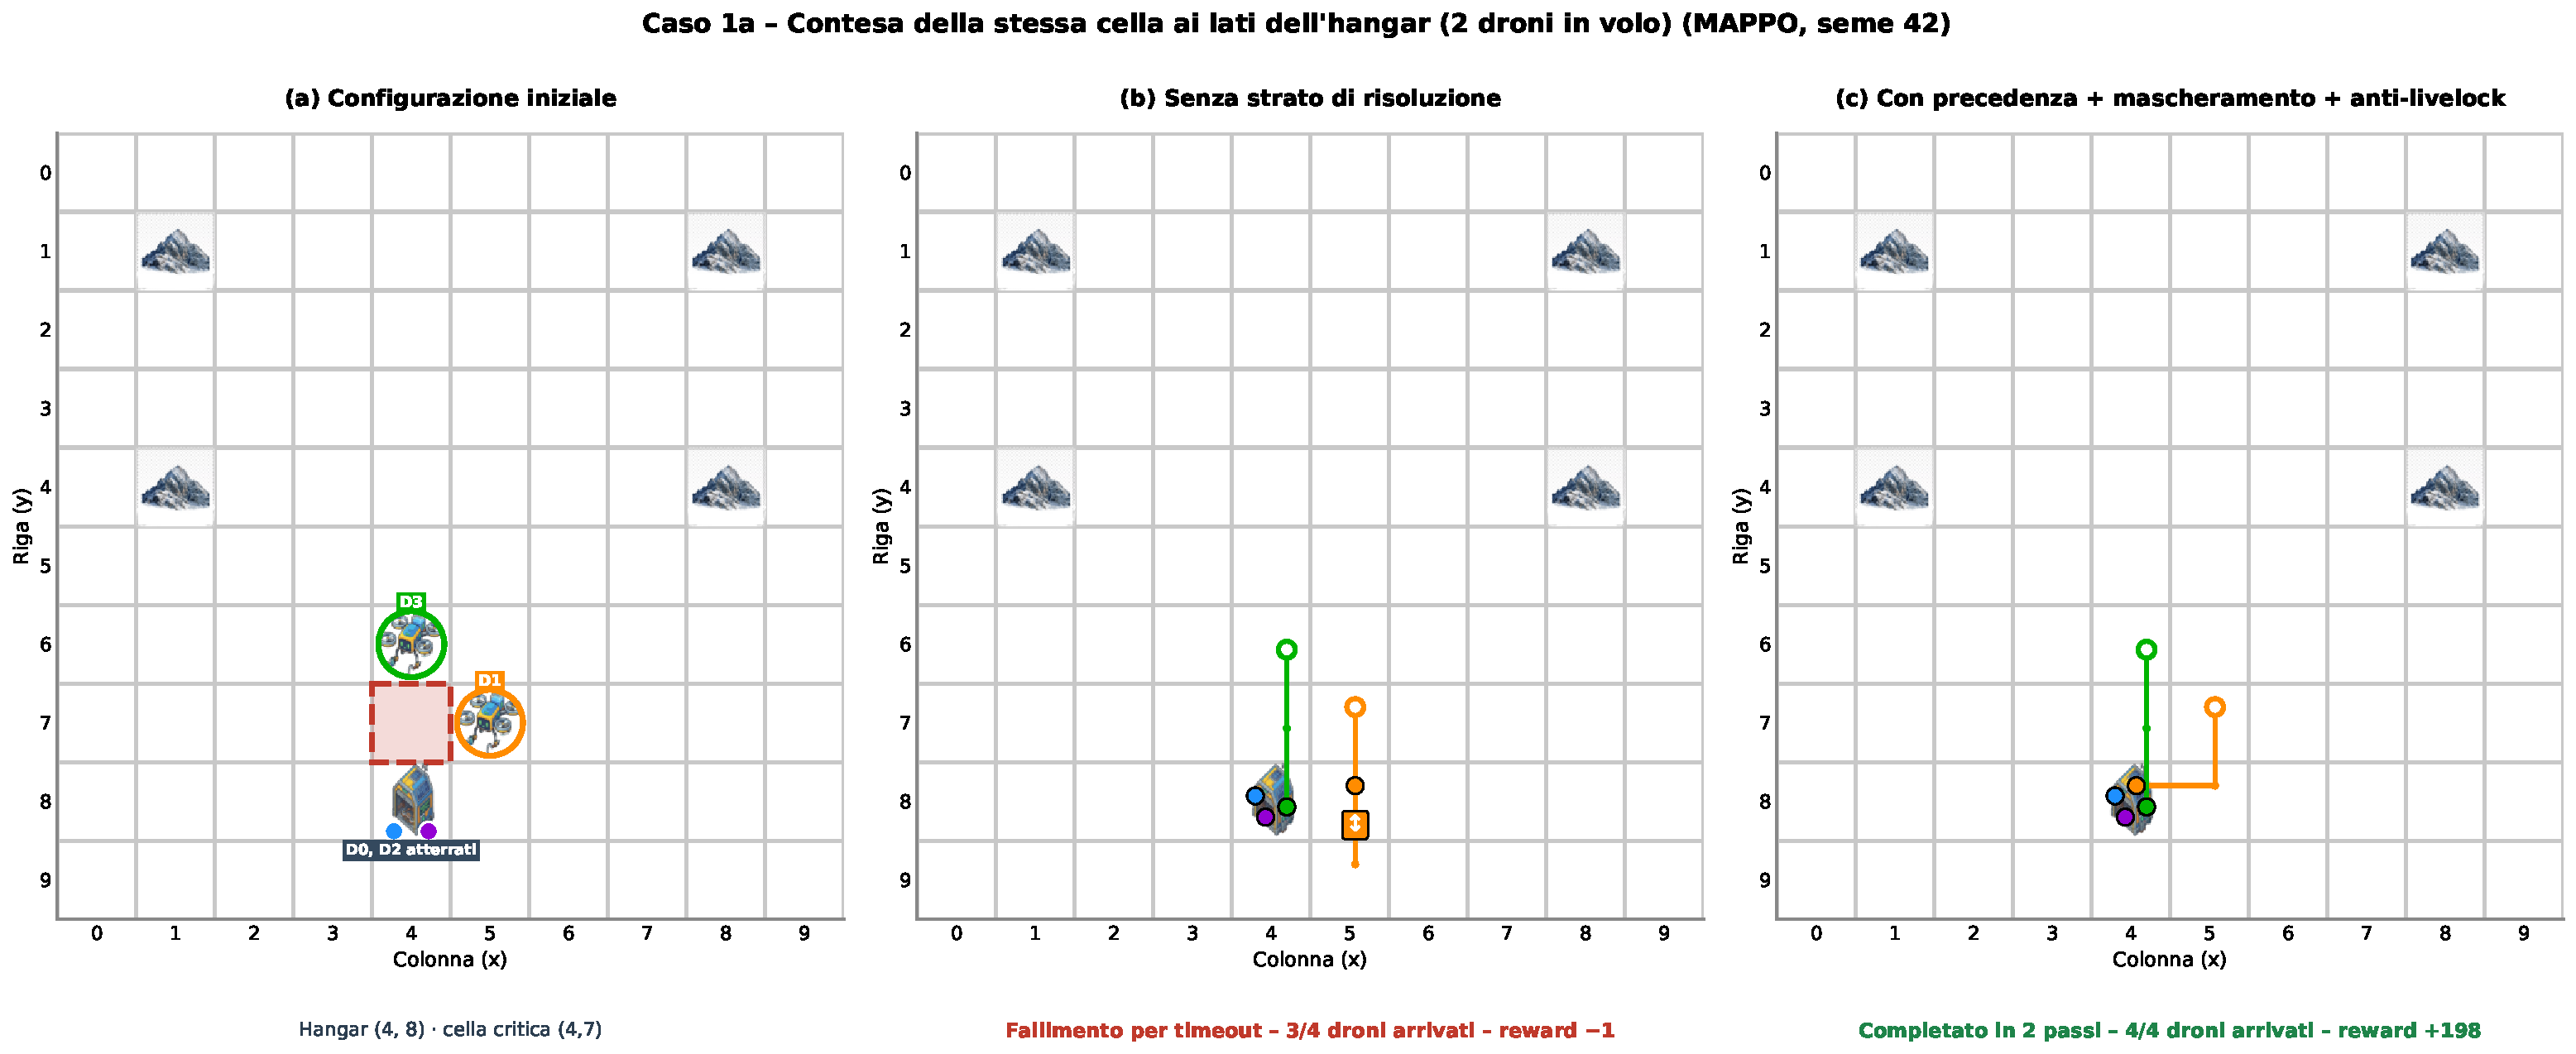
\includegraphics[width=0.95\textwidth]{fig_A_2_caso_1a_mappo.pdf}
    \caption{Caso 1a, MAPPO (seme 42): configurazione iniziale, traiettorie senza strato e con strato di risoluzione.}
    \label{fig:A_2}
\end{figure}

\begin{figure}[H]
    \centering
    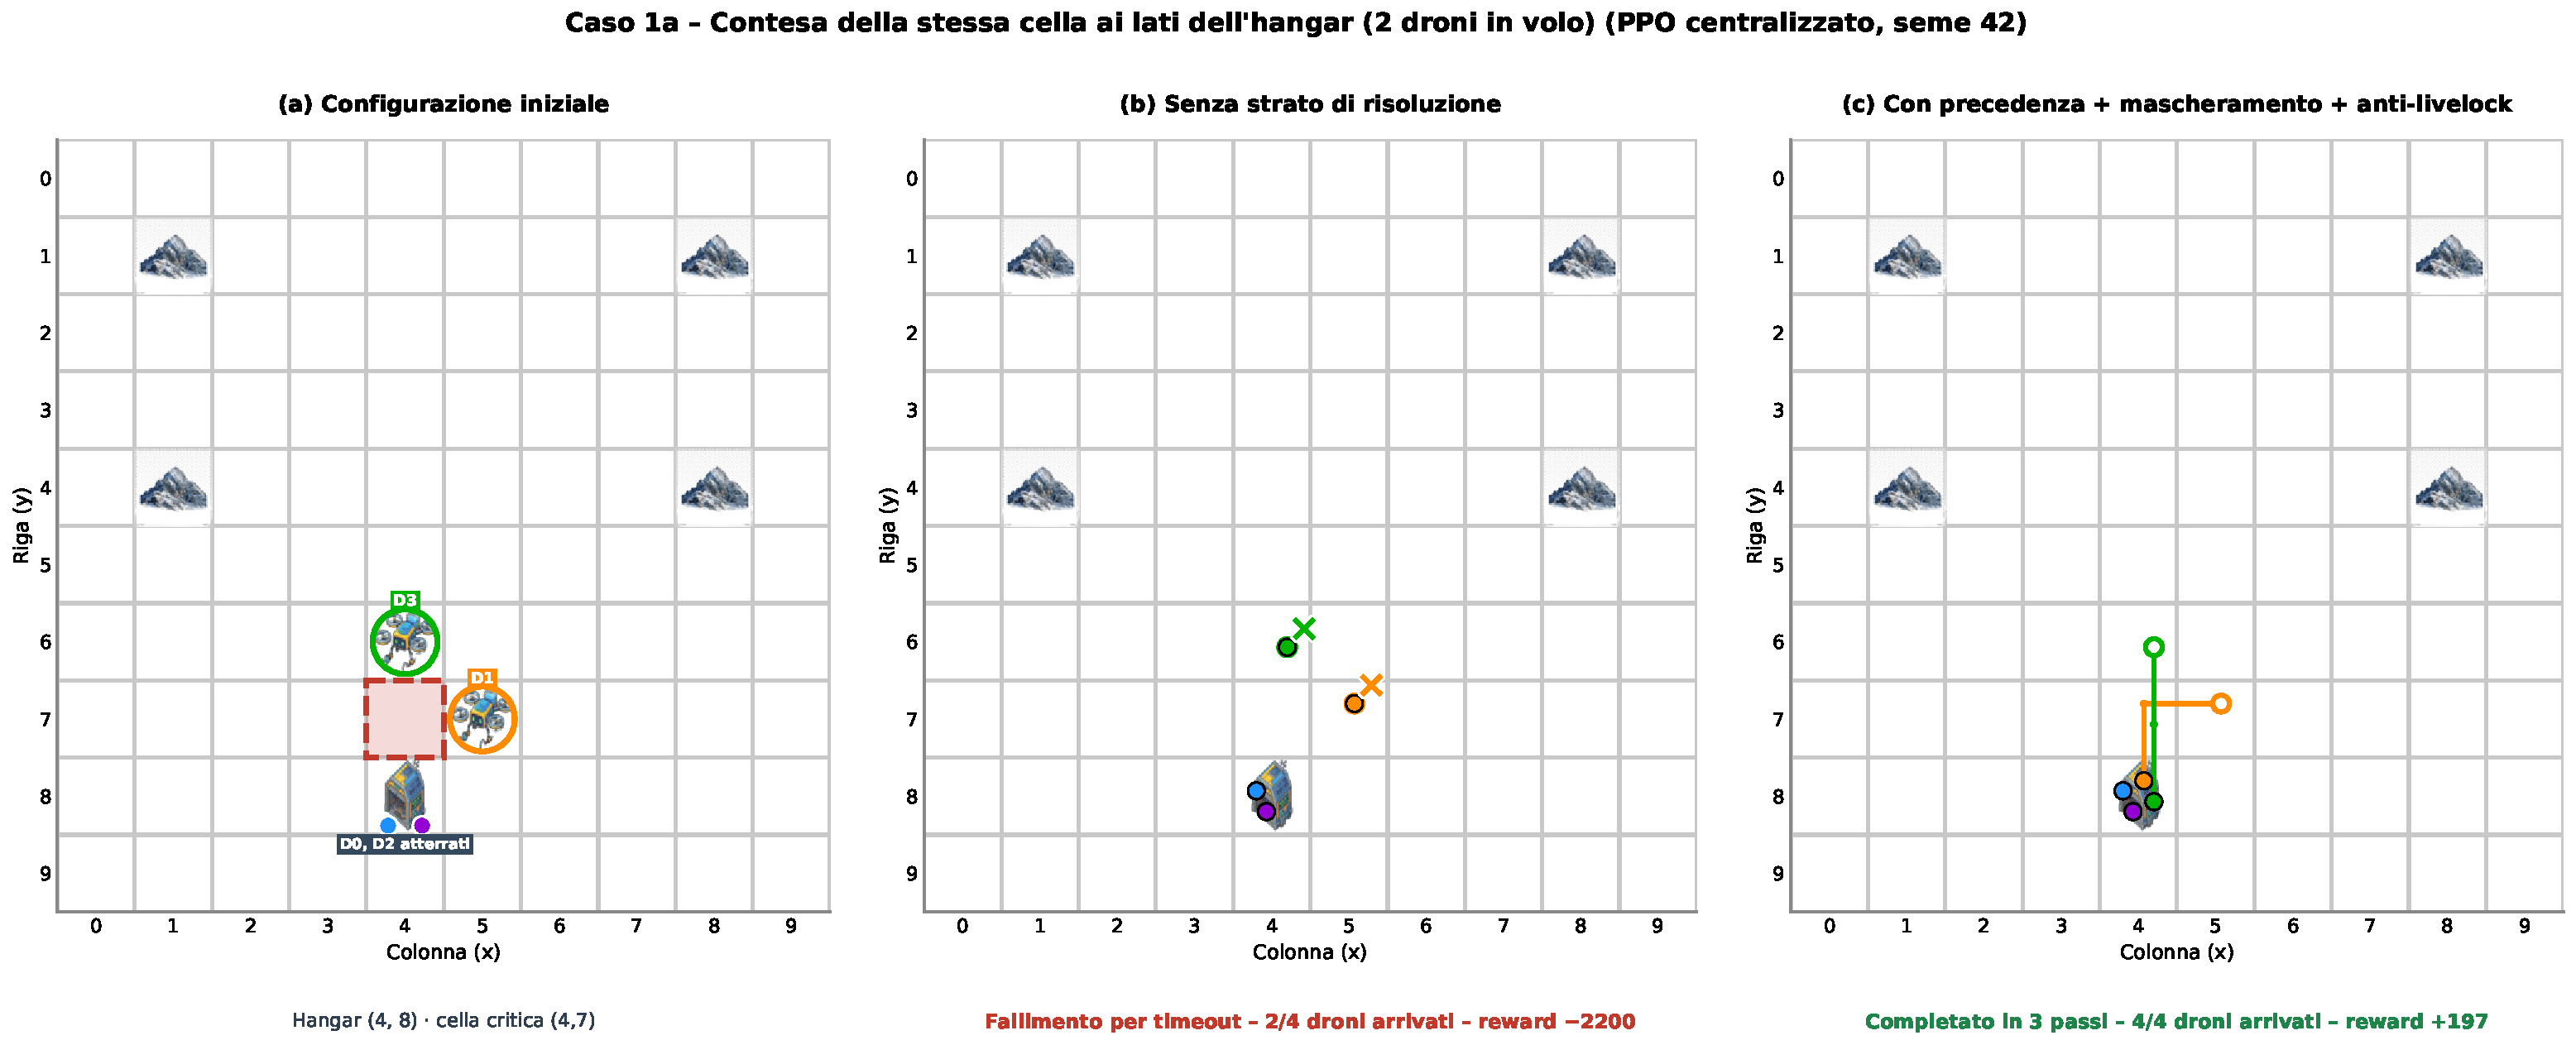
\includegraphics[width=0.95\textwidth]{fig_A_3_caso_1a_ppo.pdf}
    \caption{Caso 1a, PPO (seme 42): configurazione iniziale, traiettorie senza strato e con strato di risoluzione.}
    \label{fig:A_3}
\end{figure}

\noindent\textbf{MAPPO, senza strato di risoluzione.} Fallimento per timeout ($100$ passi) (droni arrivati: 3/4, reward: $-1$, vertex collision: $0$).

{\footnotesize
\setlength{\tabcolsep}{3.5pt}
\begin{longtable}{c l l >{\raggedright\arraybackslash}p{3.8cm}}
\toprule
\textbf{Passo} & \textbf{Posizioni ($\text{D0} \cdot \text{D1} \cdot \text{D2} \cdot \text{D3}$)} & \textbf{Azioni ($\text{D0} \cdot \text{D1} \cdot \text{D2} \cdot \text{D3}$)} & \textbf{Eventi} \\
\midrule
\endfirsthead
\toprule
\textbf{Passo} & \textbf{Posizioni ($\text{D0} \cdot \text{D1} \cdot \text{D2} \cdot \text{D3}$)} & \textbf{Azioni ($\text{D0} \cdot \text{D1} \cdot \text{D2} \cdot \text{D3}$)} & \textbf{Eventi} \\
\midrule
\endhead
\bottomrule
\endlastfoot
1      & $(4, 8) \cdot (5, 7) \cdot (4, 8) \cdot (4, 6)$ & --- $\cdot$ Giù $\cdot$ --- $\cdot$ Giù & si muovono D1, D3 \\
2      & $(4, 8) \cdot (5, 8) \cdot (4, 8) \cdot (4, 7)$ & --- $\cdot$ Giù $\cdot$ --- $\cdot$ Giù & si muovono D1, D3 \\
3      & $(4, 8) \cdot (5, 9) \cdot (4, 8) \cdot (4, 8)$ & --- $\cdot$ Su $\cdot$ --- $\cdot$ ---  & si muove D1 \\
4      & $(4, 8) \cdot (5, 8) \cdot (4, 8) \cdot (4, 8)$ & --- $\cdot$ Giù $\cdot$ --- $\cdot$ --- & si muove D1 \\
5--100 & & & D1 oscilla tra $(5, 9)$ e $(5, 8)$ \\
\end{longtable}
}

\noindent\textbf{MAPPO, con strato di risoluzione.} Completato con successo in $2$ passi (droni arrivati: 4/4, reward: $+198$, precedenze: $0$, mascheramenti: $0$, anti-livelock: $1$).

{\footnotesize
\setlength{\tabcolsep}{3.5pt}
\begin{longtable}{c l l >{\raggedright\arraybackslash}p{3.8cm}}
\toprule
\textbf{Passo} & \textbf{Posizioni ($\text{D0} \cdot \text{D1} \cdot \text{D2} \cdot \text{D3}$)} & \textbf{Azioni ($\text{D0} \cdot \text{D1} \cdot \text{D2} \cdot \text{D3}$)} & \textbf{Eventi} \\
\midrule
\endfirsthead
\toprule
\textbf{Passo} & \textbf{Posizioni ($\text{D0} \cdot \text{D1} \cdot \text{D2} \cdot \text{D3}$)} & \textbf{Azioni ($\text{D0} \cdot \text{D1} \cdot \text{D2} \cdot \text{D3}$)} & \textbf{Eventi} \\
\midrule
\endhead
\bottomrule
\endlastfoot
1 & $(4, 8) \cdot (5, 7) \cdot (4, 8) \cdot (4, 6)$ & --- $\cdot$ Giù $\cdot$ --- $\cdot$ Giù      & si muovono D1, D3 \\
2 & $(4, 8) \cdot (5, 8) \cdot (4, 8) \cdot (4, 7)$ & --- $\cdot$ Sinistra $\cdot$ --- $\cdot$ Giù & anti-livelock D1$(5, 8)$: Giù $\to$ Sinistra \\
\end{longtable}
}

\noindent\textbf{PPO, senza strato di risoluzione.} Fallimento per timeout ($100$ passi) (droni arrivati: 2/4, reward: $-2200$, vertex collision: $100$).

{\footnotesize
\setlength{\tabcolsep}{3.5pt}
\begin{longtable}{c l l >{\raggedright\arraybackslash}p{3.8cm}}
\toprule
\textbf{Passo} & \textbf{Posizioni ($\text{D0} \cdot \text{D1} \cdot \text{D2} \cdot \text{D3}$)} & \textbf{Azioni ($\text{D0} \cdot \text{D1} \cdot \text{D2} \cdot \text{D3}$)} & \textbf{Eventi} \\
\midrule
\endfirsthead
\toprule
\textbf{Passo} & \textbf{Posizioni ($\text{D0} \cdot \text{D1} \cdot \text{D2} \cdot \text{D3}$)} & \textbf{Azioni ($\text{D0} \cdot \text{D1} \cdot \text{D2} \cdot \text{D3}$)} & \textbf{Eventi} \\
\midrule
\endhead
\bottomrule
\endlastfoot
1      & $(4, 8) \cdot (5, 7) \cdot (4, 8) \cdot (4, 6)$ & --- $\cdot$ Sinistra $\cdot$ --- $\cdot$ Giù & scontro D1$(5, 7)$ / D3$(4, 6)$ su $(4, 7)$ accanto all'hangar \\
2--100 & & & D1 resta fermo in $(5, 7)$; D3 resta fermo in $(4, 6)$ \\
\end{longtable}
}

\noindent\textbf{PPO, con strato di risoluzione.} Completato con successo in $3$ passi (droni arrivati: 4/4, reward: $+197$, precedenze: $1$, mascheramenti: $0$, anti-livelock: $2$).

{\footnotesize
\setlength{\tabcolsep}{3.5pt}
\begin{longtable}{c l l >{\raggedright\arraybackslash}p{3.8cm}}
\toprule
\textbf{Passo} & \textbf{Posizioni ($\text{D0} \cdot \text{D1} \cdot \text{D2} \cdot \text{D3}$)} & \textbf{Azioni ($\text{D0} \cdot \text{D1} \cdot \text{D2} \cdot \text{D3}$)} & \textbf{Eventi} \\
\midrule
\endfirsthead
\toprule
\textbf{Passo} & \textbf{Posizioni ($\text{D0} \cdot \text{D1} \cdot \text{D2} \cdot \text{D3}$)} & \textbf{Azioni ($\text{D0} \cdot \text{D1} \cdot \text{D2} \cdot \text{D3}$)} & \textbf{Eventi} \\
\midrule
\endhead
\bottomrule
\endlastfoot
1 & $(4, 8) \cdot (5, 7) \cdot (4, 8) \cdot (4, 6)$ & --- $\cdot$ Sinistra $\cdot$ --- $\cdot$ Giù & precedenza su $(4, 7)$: passa D1 (distanza $2$), attende D3 (distanza $2$) \\
2 & $(4, 8) \cdot (4, 7) \cdot (4, 8) \cdot (4, 6)$ & --- $\cdot$ Giù $\cdot$ --- $\cdot$ Giù      & anti-livelock D1$(4, 7)$: Sinistra $\to$ Giù \\
3 & $(4, 8) \cdot (4, 8) \cdot (4, 8) \cdot (4, 7)$ & --- $\cdot$ --- $\cdot$ --- $\cdot$ Giù      & anti-livelock D3$(4, 7)$: Sinistra $\to$ Giù \\
\end{longtable}
}

% -----------------------------------------------------------------------------
% CASO 1B
% -----------------------------------------------------------------------------
\section{Caso 1b -- Contesa ai lati dell'hangar con 4 droni}
\label{sec:app_caso_1b}

Hangar in $(5,5)$ con montagne sopra $(5,4)$ e sotto $(5,6)$. D0$(3,5)$ e D1$(4,4)$ puntano al lato sinistro $(4,5)$, mentre D2$(7,5)$ e D3$(6,6)$ puntano al lato destro $(6,5)$.

\begin{figure}[H]
    \centering
    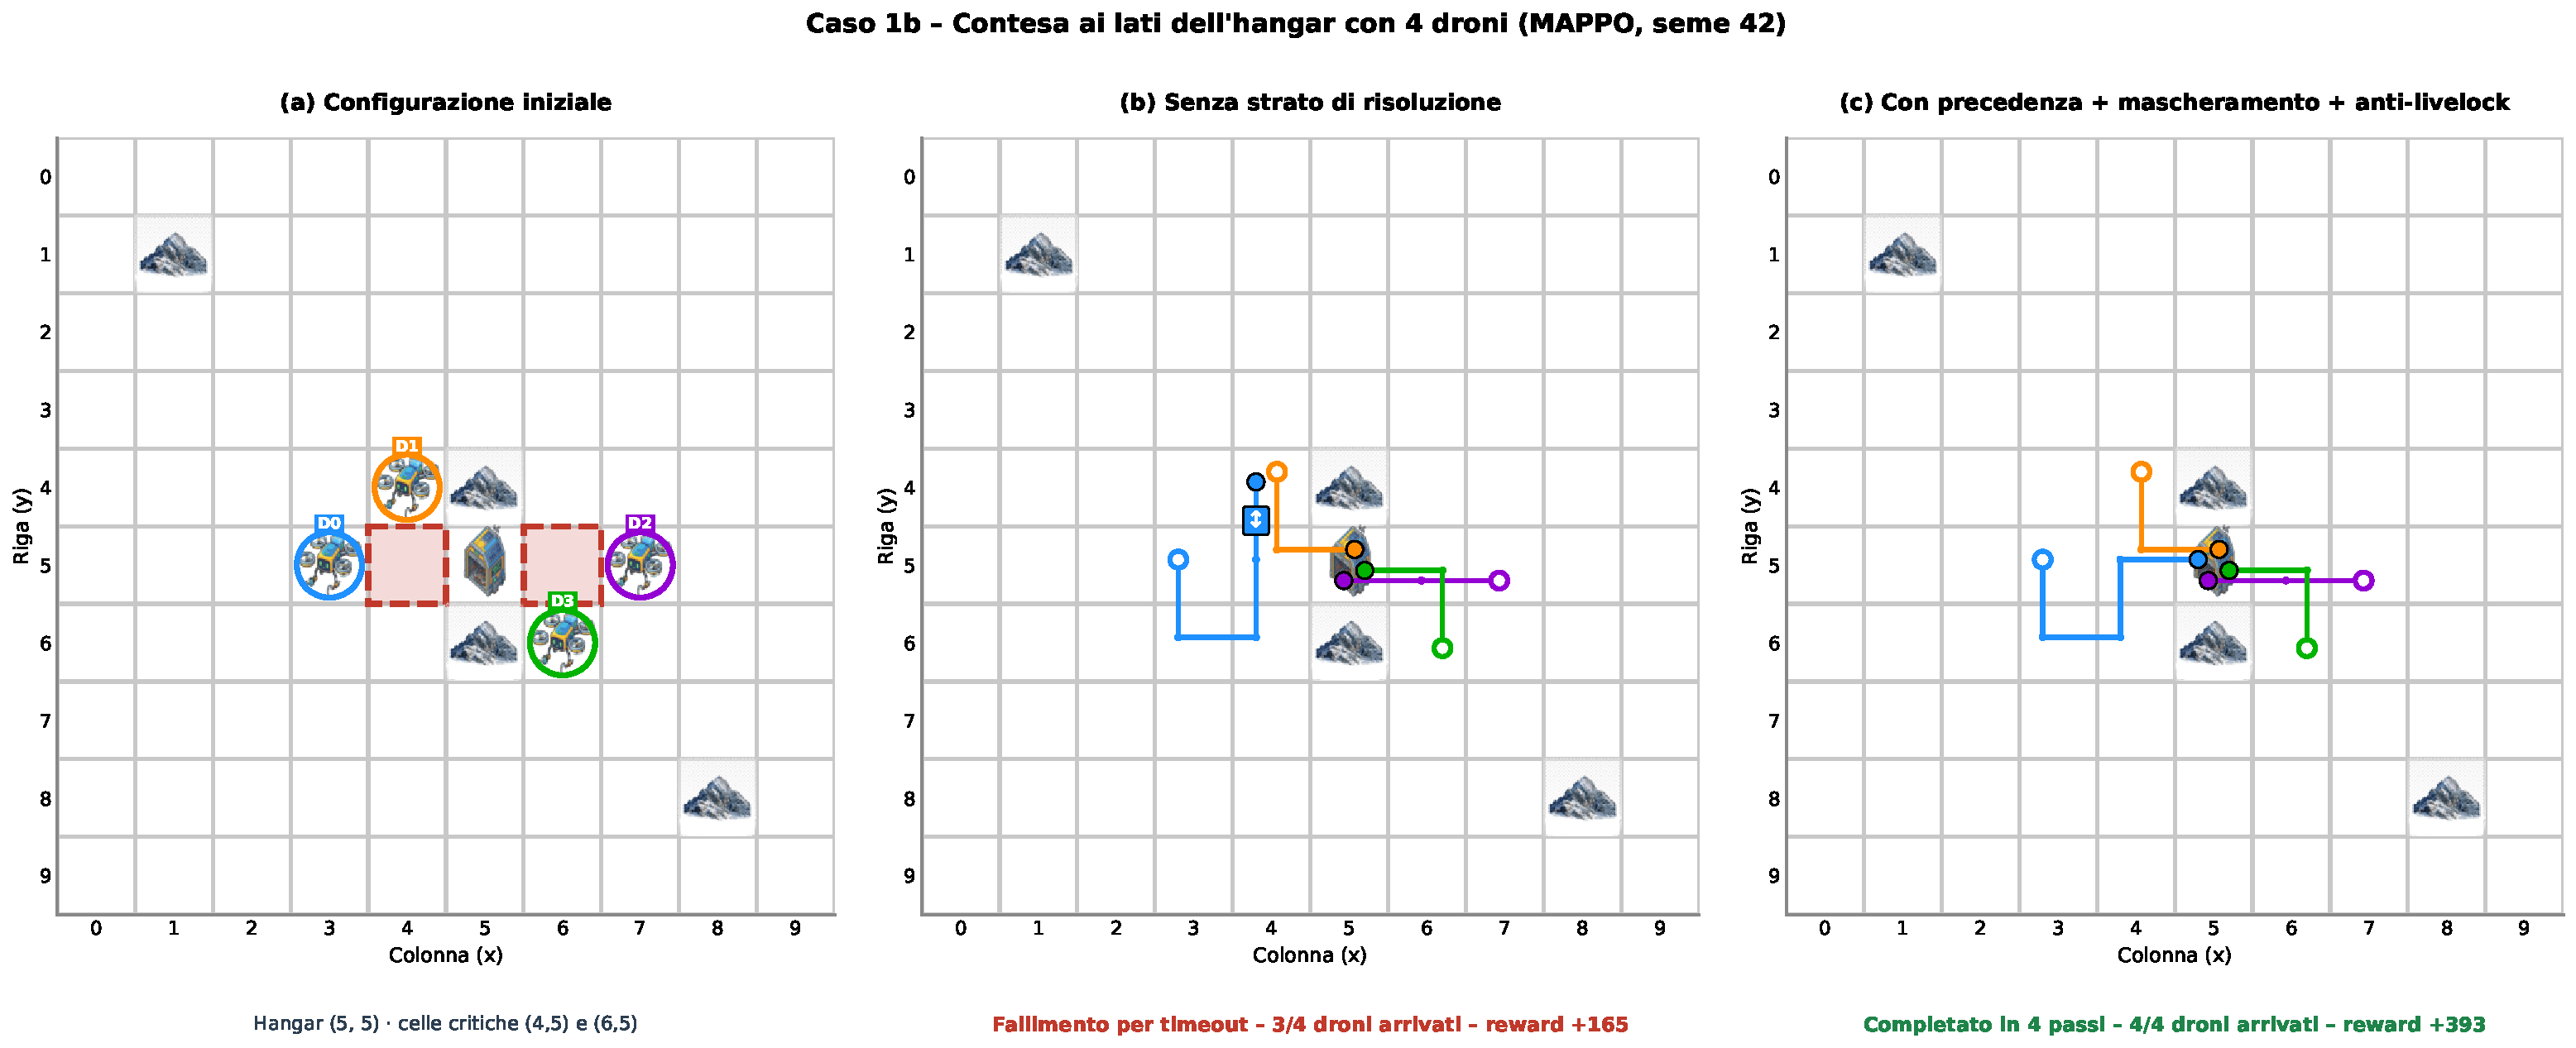
\includegraphics[width=0.95\textwidth]{fig_A_4_caso_1b_mappo.pdf}
    \caption{Caso 1b, MAPPO (seme 42): configurazione iniziale, traiettorie senza strato e con strato di risoluzione.}
    \label{fig:A_4}
\end{figure}

\begin{figure}[H]
    \centering
    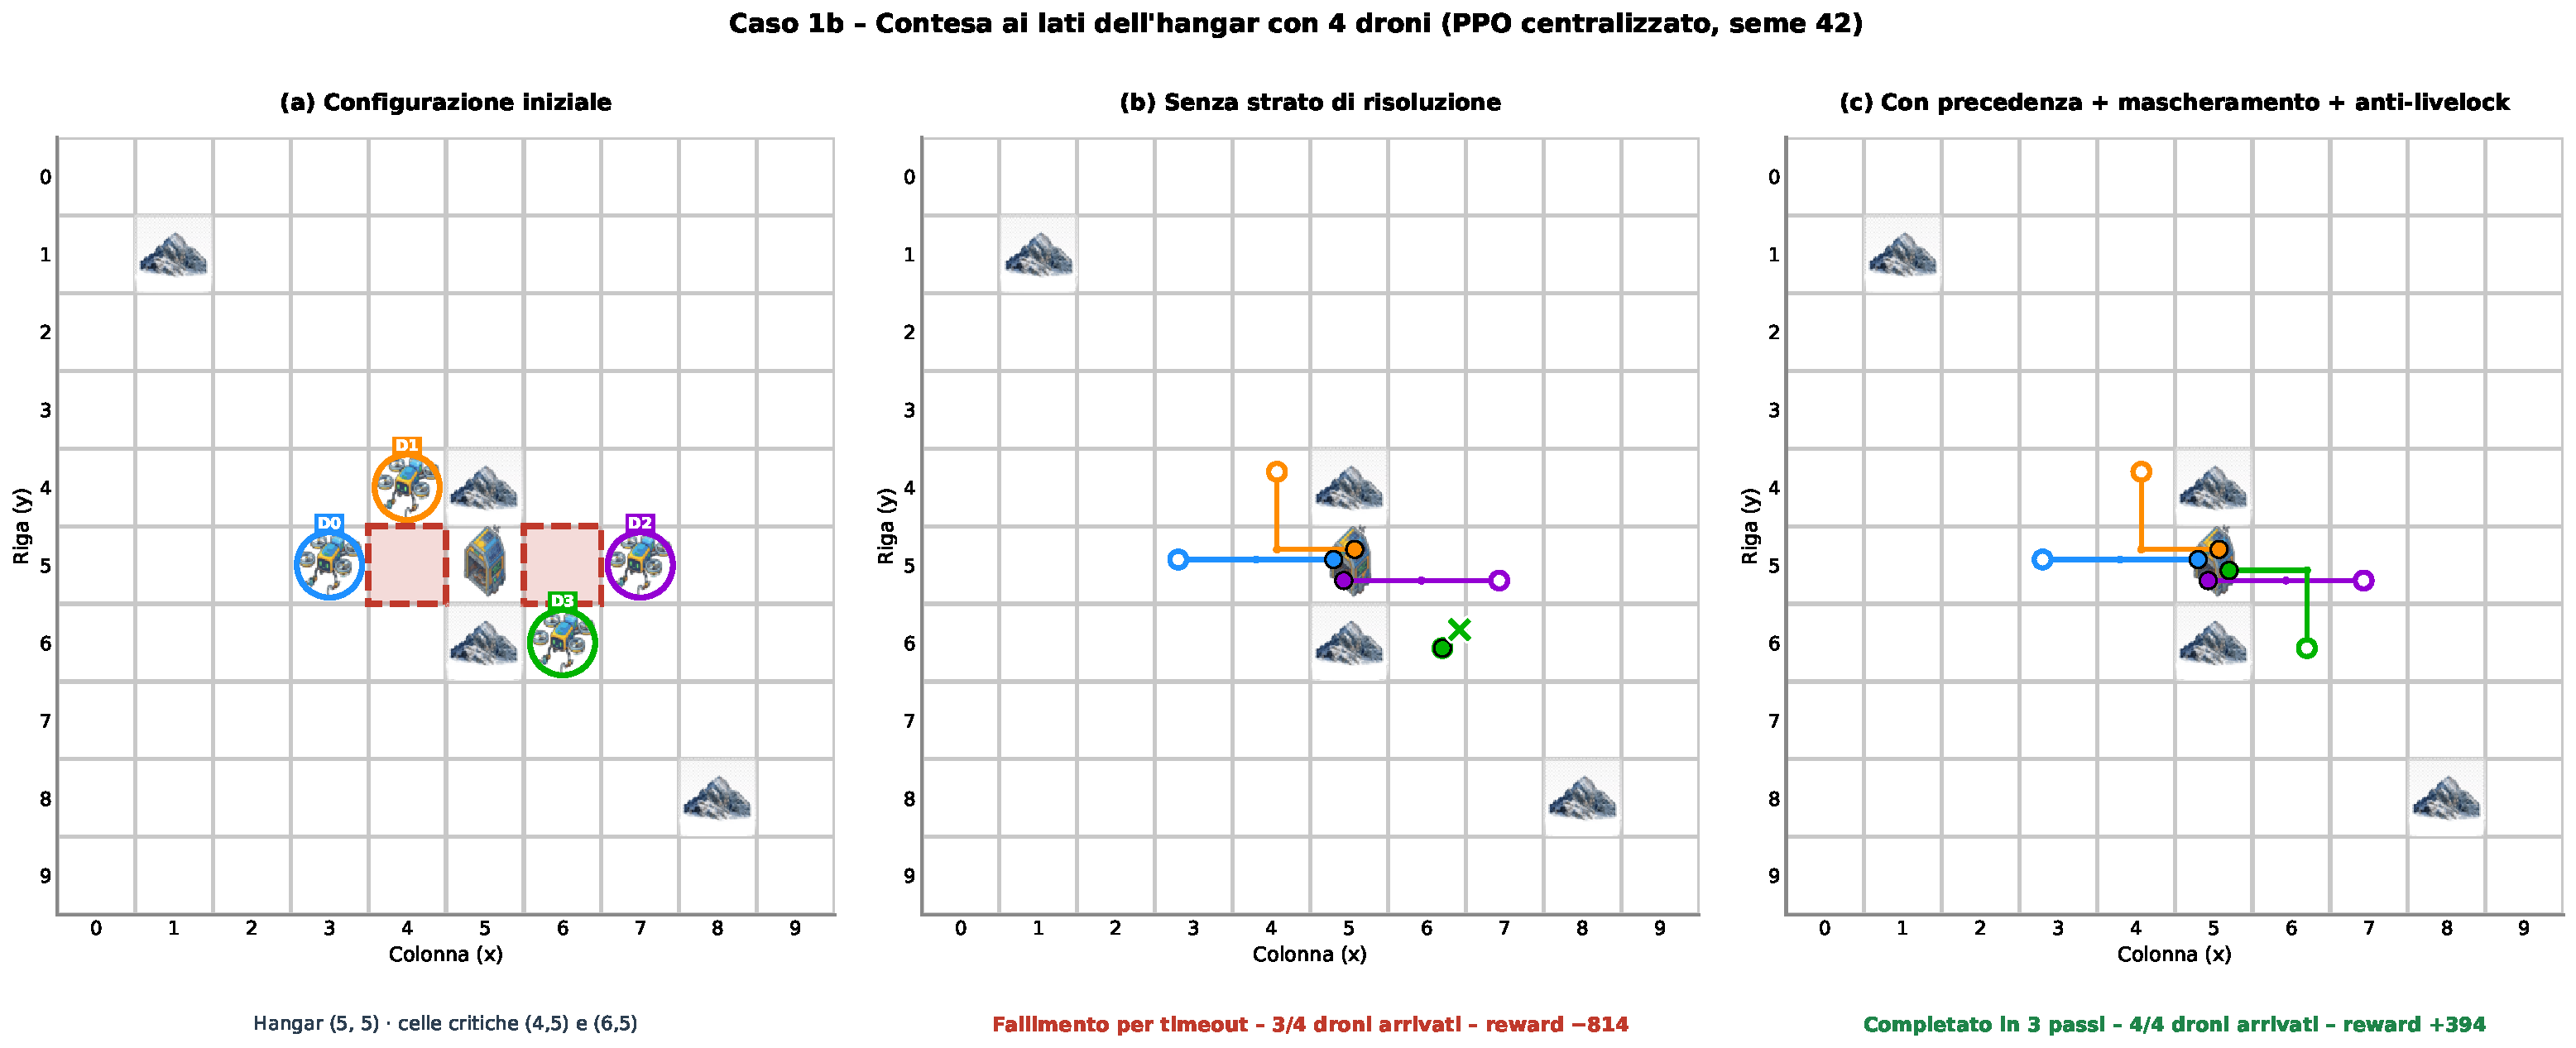
\includegraphics[width=0.95\textwidth]{fig_A_5_caso_1b_ppo.pdf}
    \caption{Caso 1b, PPO (seme 42): configurazione iniziale, traiettorie senza strato e con strato di risoluzione.}
    \label{fig:A_5}
\end{figure}

\noindent\textbf{MAPPO, senza strato di risoluzione.} Fallimento per timeout ($100$ passi) (droni arrivati: 3/4, reward: $+165$, vertex collision: $1$).

{\footnotesize
\setlength{\tabcolsep}{3.5pt}
\begin{longtable}{c l l >{\raggedright\arraybackslash}p{3.8cm}}
\toprule
\textbf{Passo} & \textbf{Posizioni ($\text{D0} \cdot \text{D1} \cdot \text{D2} \cdot \text{D3}$)} & \textbf{Azioni ($\text{D0} \cdot \text{D1} \cdot \text{D2} \cdot \text{D3}$)} & \textbf{Eventi} \\
\midrule
\endfirsthead
\toprule
\textbf{Passo} & \textbf{Posizioni ($\text{D0} \cdot \text{D1} \cdot \text{D2} \cdot \text{D3}$)} & \textbf{Azioni ($\text{D0} \cdot \text{D1} \cdot \text{D2} \cdot \text{D3}$)} & \textbf{Eventi} \\
\midrule
\endhead
\bottomrule
\endlastfoot
1      & $(3, 5) \cdot (4, 4) \cdot (7, 5) \cdot (6, 6)$ & Giù $\cdot$ Giù $\cdot$ Sinistra $\cdot$ Sinistra & D3$(6, 6)$ urta la montagna in $(5, 6)$ \\
2      & $(3, 6) \cdot (4, 5) \cdot (6, 5) \cdot (6, 6)$ & Destra $\cdot$ Giù $\cdot$ Sinistra $\cdot$ Su    & scontro D0$(3, 6)$ / D1$(4, 5)$ su $(4, 6)$ \\
3      & $(3, 6) \cdot (4, 5) \cdot (5, 5) \cdot (6, 5)$ & Destra $\cdot$ Destra $\cdot$ --- $\cdot$ Sinistra & si muovono D0, D1, D3 \\
4      & $(4, 6) \cdot (5, 5) \cdot (5, 5) \cdot (5, 5)$ & Su $\cdot$ --- $\cdot$ --- $\cdot$ ---            & si muove D0 \\
5      & $(4, 5) \cdot (5, 5) \cdot (5, 5) \cdot (5, 5)$ & Su $\cdot$ --- $\cdot$ --- $\cdot$ ---            & si muove D0 \\
6      & $(4, 4) \cdot (5, 5) \cdot (5, 5) \cdot (5, 5)$ & Giù $\cdot$ --- $\cdot$ --- $\cdot$ ---           & si muove D0 \\
7--100 & & & D0 oscilla tra $(4, 5)$ e $(4, 4)$ \\
\end{longtable}
}

\noindent\textbf{MAPPO, con strato di risoluzione.} Completato con successo in $4$ passi (droni arrivati: 4/4, reward: $+393$, precedenze: $1$, mascheramenti: $1$, anti-livelock: $3$).

{\footnotesize
\setlength{\tabcolsep}{3.5pt}
\begin{longtable}{c l l >{\raggedright\arraybackslash}p{3.8cm}}
\toprule
\textbf{Passo} & \textbf{Posizioni ($\text{D0} \cdot \text{D1} \cdot \text{D2} \cdot \text{D3}$)} & \textbf{Azioni ($\text{D0} \cdot \text{D1} \cdot \text{D2} \cdot \text{D3}$)} & \textbf{Eventi} \\
\midrule
\endfirsthead
\toprule
\textbf{Passo} & \textbf{Posizioni ($\text{D0} \cdot \text{D1} \cdot \text{D2} \cdot \text{D3}$)} & \textbf{Azioni ($\text{D0} \cdot \text{D1} \cdot \text{D2} \cdot \text{D3}$)} & \textbf{Eventi} \\
\midrule
\endhead
\bottomrule
\endlastfoot
1 & $(3, 5) \cdot (4, 4) \cdot (7, 5) \cdot (6, 6)$ & Giù $\cdot$ Giù $\cdot$ Sinistra $\cdot$ Su       & mascheramento D3$(6, 6)$: Sinistra $\to$ Su; precedenza su $(6, 5)$: passa D2 (distanza $2$), attende D3 (distanza $2$) \\
2 & $(3, 6) \cdot (4, 5) \cdot (6, 5) \cdot (6, 6)$ & Destra $\cdot$ Destra $\cdot$ Sinistra $\cdot$ Su & anti-livelock D1$(4, 5)$: Giù $\to$ Destra \\
3 & $(4, 6) \cdot (5, 5) \cdot (5, 5) \cdot (6, 5)$ & Su $\cdot$ --- $\cdot$ --- $\cdot$ Sinistra       & anti-livelock D3$(6, 5)$: Giù $\to$ Sinistra \\
4 & $(4, 5) \cdot (5, 5) \cdot (5, 5) \cdot (5, 5)$ & Destra $\cdot$ --- $\cdot$ --- $\cdot$ ---        & anti-livelock D0$(4, 5)$: Su $\to$ Destra \\
\end{longtable}
}

\noindent\textbf{PPO, senza strato di risoluzione.} Fallimento per timeout ($100$ passi) (droni arrivati: 3/4, reward: $-814$, vertex collision: $0$).

{\footnotesize
\setlength{\tabcolsep}{3.5pt}
\begin{longtable}{c l l >{\raggedright\arraybackslash}p{3.8cm}}
\toprule
\textbf{Passo} & \textbf{Posizioni ($\text{D0} \cdot \text{D1} \cdot \text{D2} \cdot \text{D3}$)} & \textbf{Azioni ($\text{D0} \cdot \text{D1} \cdot \text{D2} \cdot \text{D3}$)} & \textbf{Eventi} \\
\midrule
\endfirsthead
\toprule
\textbf{Passo} & \textbf{Posizioni ($\text{D0} \cdot \text{D1} \cdot \text{D2} \cdot \text{D3}$)} & \textbf{Azioni ($\text{D0} \cdot \text{D1} \cdot \text{D2} \cdot \text{D3}$)} & \textbf{Eventi} \\
\midrule
\endhead
\bottomrule
\endlastfoot
1      & $(3, 5) \cdot (4, 4) \cdot (7, 5) \cdot (6, 6)$ & Destra $\cdot$ Destra $\cdot$ Sinistra $\cdot$ Sinistra & D1$(4, 4)$ urta la montagna in $(5, 4)$; D3$(6, 6)$ urta la montagna in $(5, 6)$ \\
2      & $(4, 5) \cdot (4, 4) \cdot (6, 5) \cdot (6, 6)$ & Destra $\cdot$ Giù $\cdot$ Sinistra $\cdot$ Sinistra    & D3$(6, 6)$ urta la montagna in $(5, 6)$ \\
3      & $(5, 5) \cdot (4, 5) \cdot (5, 5) \cdot (6, 6)$ & --- $\cdot$ Destra $\cdot$ --- $\cdot$ Sinistra         & D3$(6, 6)$ urta la montagna in $(5, 6)$ \\
4      & $(5, 5) \cdot (5, 5) \cdot (5, 5) \cdot (6, 6)$ & --- $\cdot$ --- $\cdot$ --- $\cdot$ Sinistra            & D3$(6, 6)$ urta la montagna in $(5, 6)$ \\
5--100 & & & D3 resta fermo in $(6, 6)$ \\
\end{longtable}
}

\noindent\textbf{PPO, con strato di risoluzione.} Completato con successo in $3$ passi (droni arrivati: 4/4, reward: $+394$, precedenze: $2$, mascheramenti: $3$, anti-livelock: $0$).

{\footnotesize
\setlength{\tabcolsep}{3.5pt}
\begin{longtable}{c l l >{\raggedright\arraybackslash}p{3.8cm}}
\toprule
\textbf{Passo} & \textbf{Posizioni ($\text{D0} \cdot \text{D1} \cdot \text{D2} \cdot \text{D3}$)} & \textbf{Azioni ($\text{D0} \cdot \text{D1} \cdot \text{D2} \cdot \text{D3}$)} & \textbf{Eventi} \\
\midrule
\endfirsthead
\toprule
\textbf{Passo} & \textbf{Posizioni ($\text{D0} \cdot \text{D1} \cdot \text{D2} \cdot \text{D3}$)} & \textbf{Azioni ($\text{D0} \cdot \text{D1} \cdot \text{D2} \cdot \text{D3}$)} & \textbf{Eventi} \\
\midrule
\endhead
\bottomrule
\endlastfoot
1 & $(3, 5) \cdot (4, 4) \cdot (7, 5) \cdot (6, 6)$ & Destra $\cdot$ Giù $\cdot$ Sinistra $\cdot$ Su & mascheramento D1$(4, 4)$: Destra $\to$ Giù; mascheramento D3$(6, 6)$: Sinistra $\to$ Su; precedenza su $(4, 5)$: passa D0 (distanza $2$), attende D1 (distanza $2$); precedenza su $(6, 5)$: passa D2 (distanza $2$), attende D3 (distanza $2$) \\
2 & $(4, 5) \cdot (4, 4) \cdot (6, 5) \cdot (6, 6)$ & Destra $\cdot$ Giù $\cdot$ Sinistra $\cdot$ Su & mascheramento D3$(6, 6)$: Sinistra $\to$ Su \\
3 & $(5, 5) \cdot (4, 5) \cdot (5, 5) \cdot (6, 5)$ & --- $\cdot$ Destra $\cdot$ --- $\cdot$ Sinistra & si muovono D1, D3 \\
\end{longtable}
}

% -----------------------------------------------------------------------------
% CASO 2A
% -----------------------------------------------------------------------------
\section{Caso 2a -- Montagne a 1 cella dal bordo sinistro}
\label{sec:app_caso_2a}

Montagne in $(1,5)$, $(2,5)$, $(3,5)$, $(4,5)$ che lasciano solo la cella $(0,5)$ libera sul bordo sinistro. Hangar in $(0,7)$ e droni in $(0,4)$, $(1,4)$, $(0,3)$ e $(2,4)$ che devono passare da $(0,5)$.

\begin{figure}[H]
    \centering
    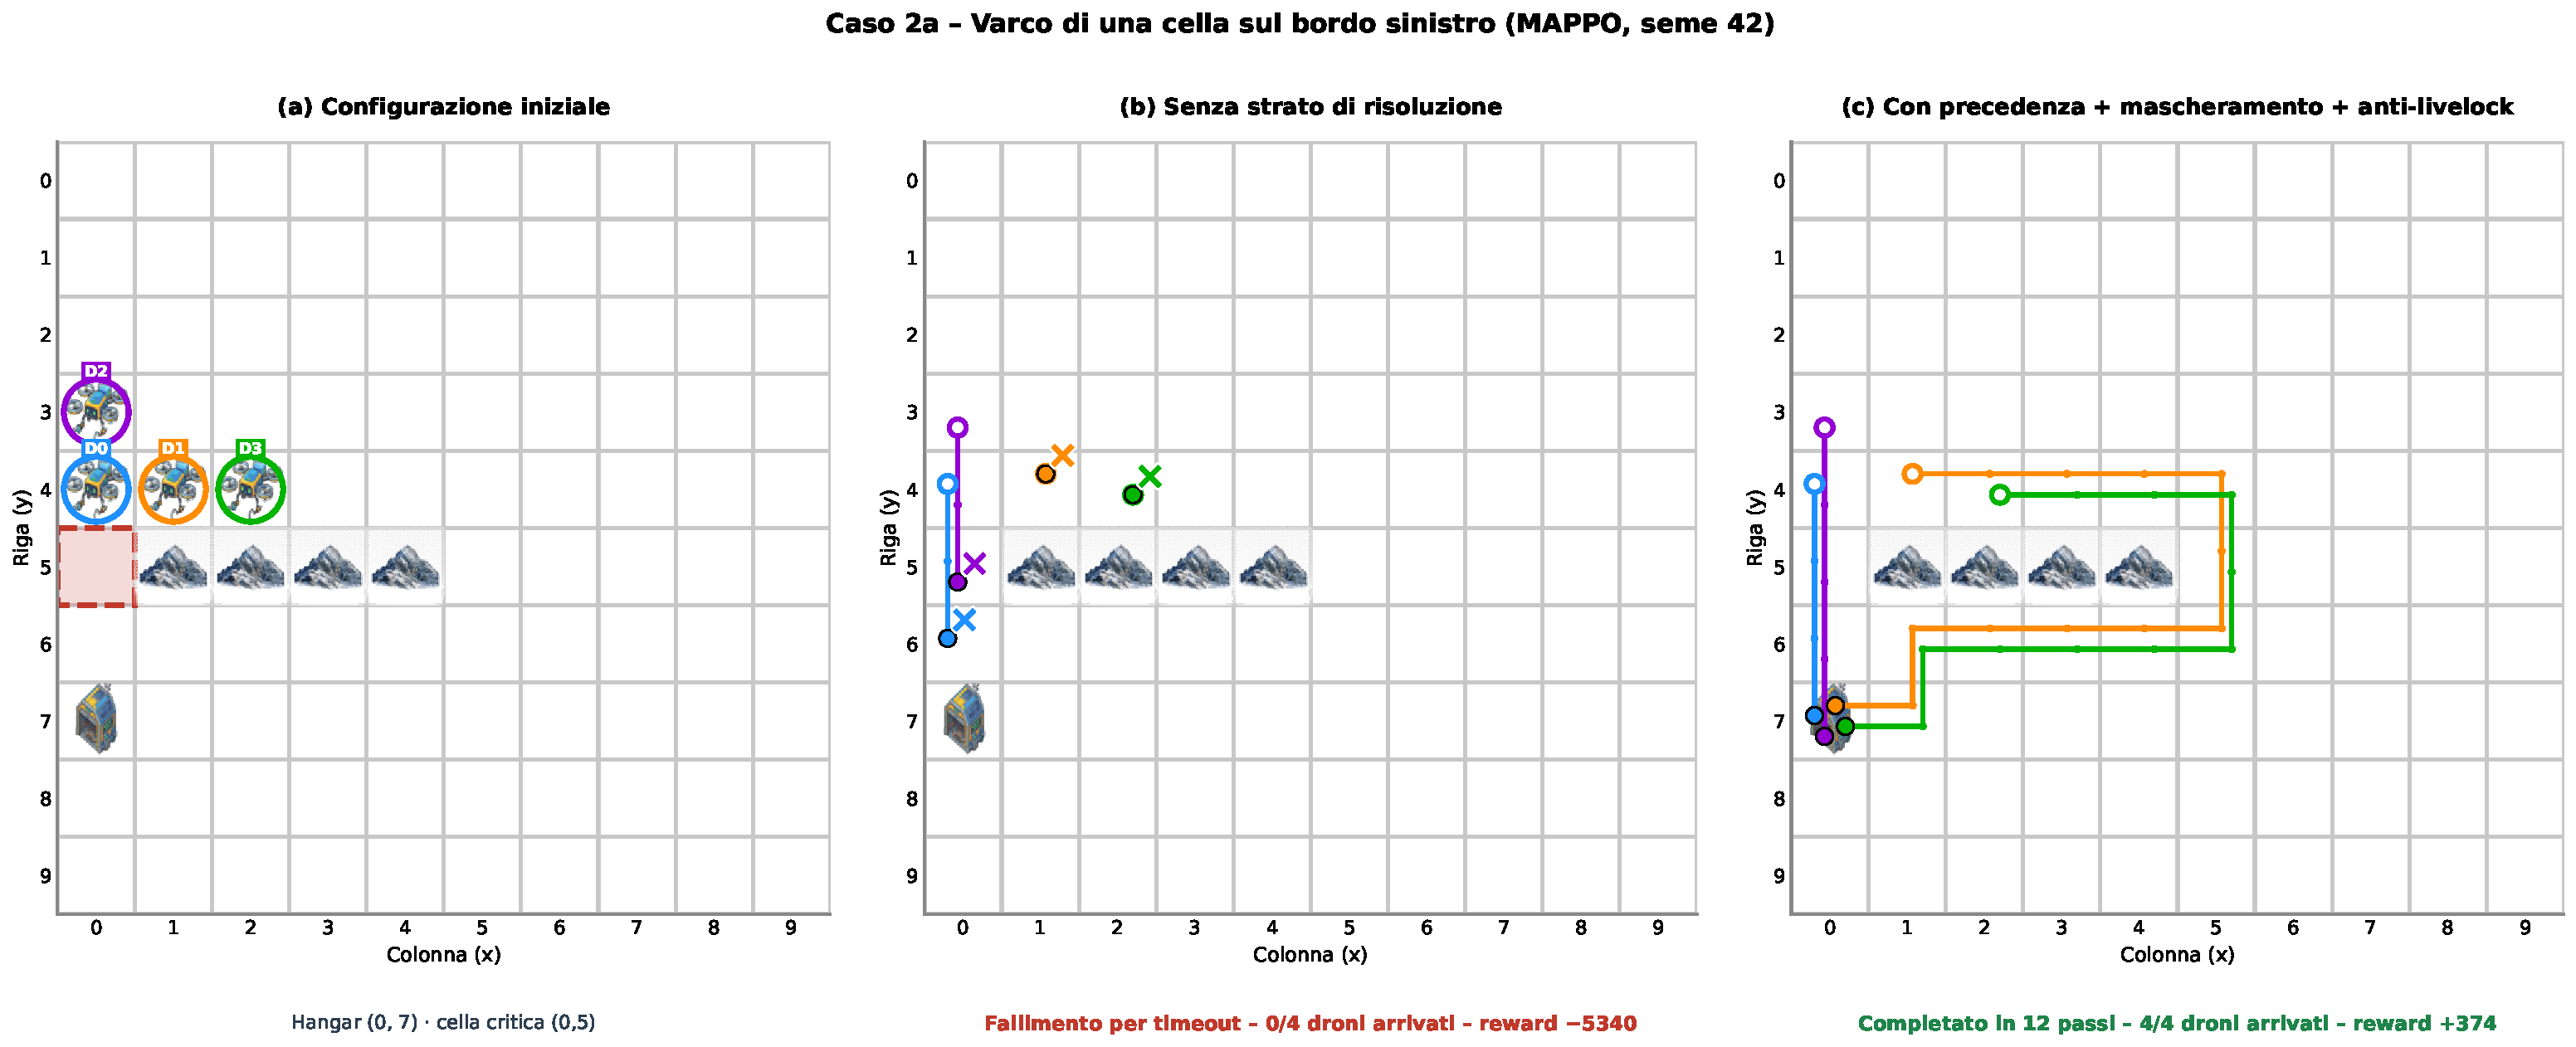
\includegraphics[width=0.95\textwidth]{fig_A_6_caso_2a_mappo.pdf}
    \caption{Caso 2a, MAPPO (seme 42): configurazione iniziale, traiettorie senza strato e con strato di risoluzione.}
    \label{fig:A_6}
\end{figure}

\begin{figure}[H]
    \centering
    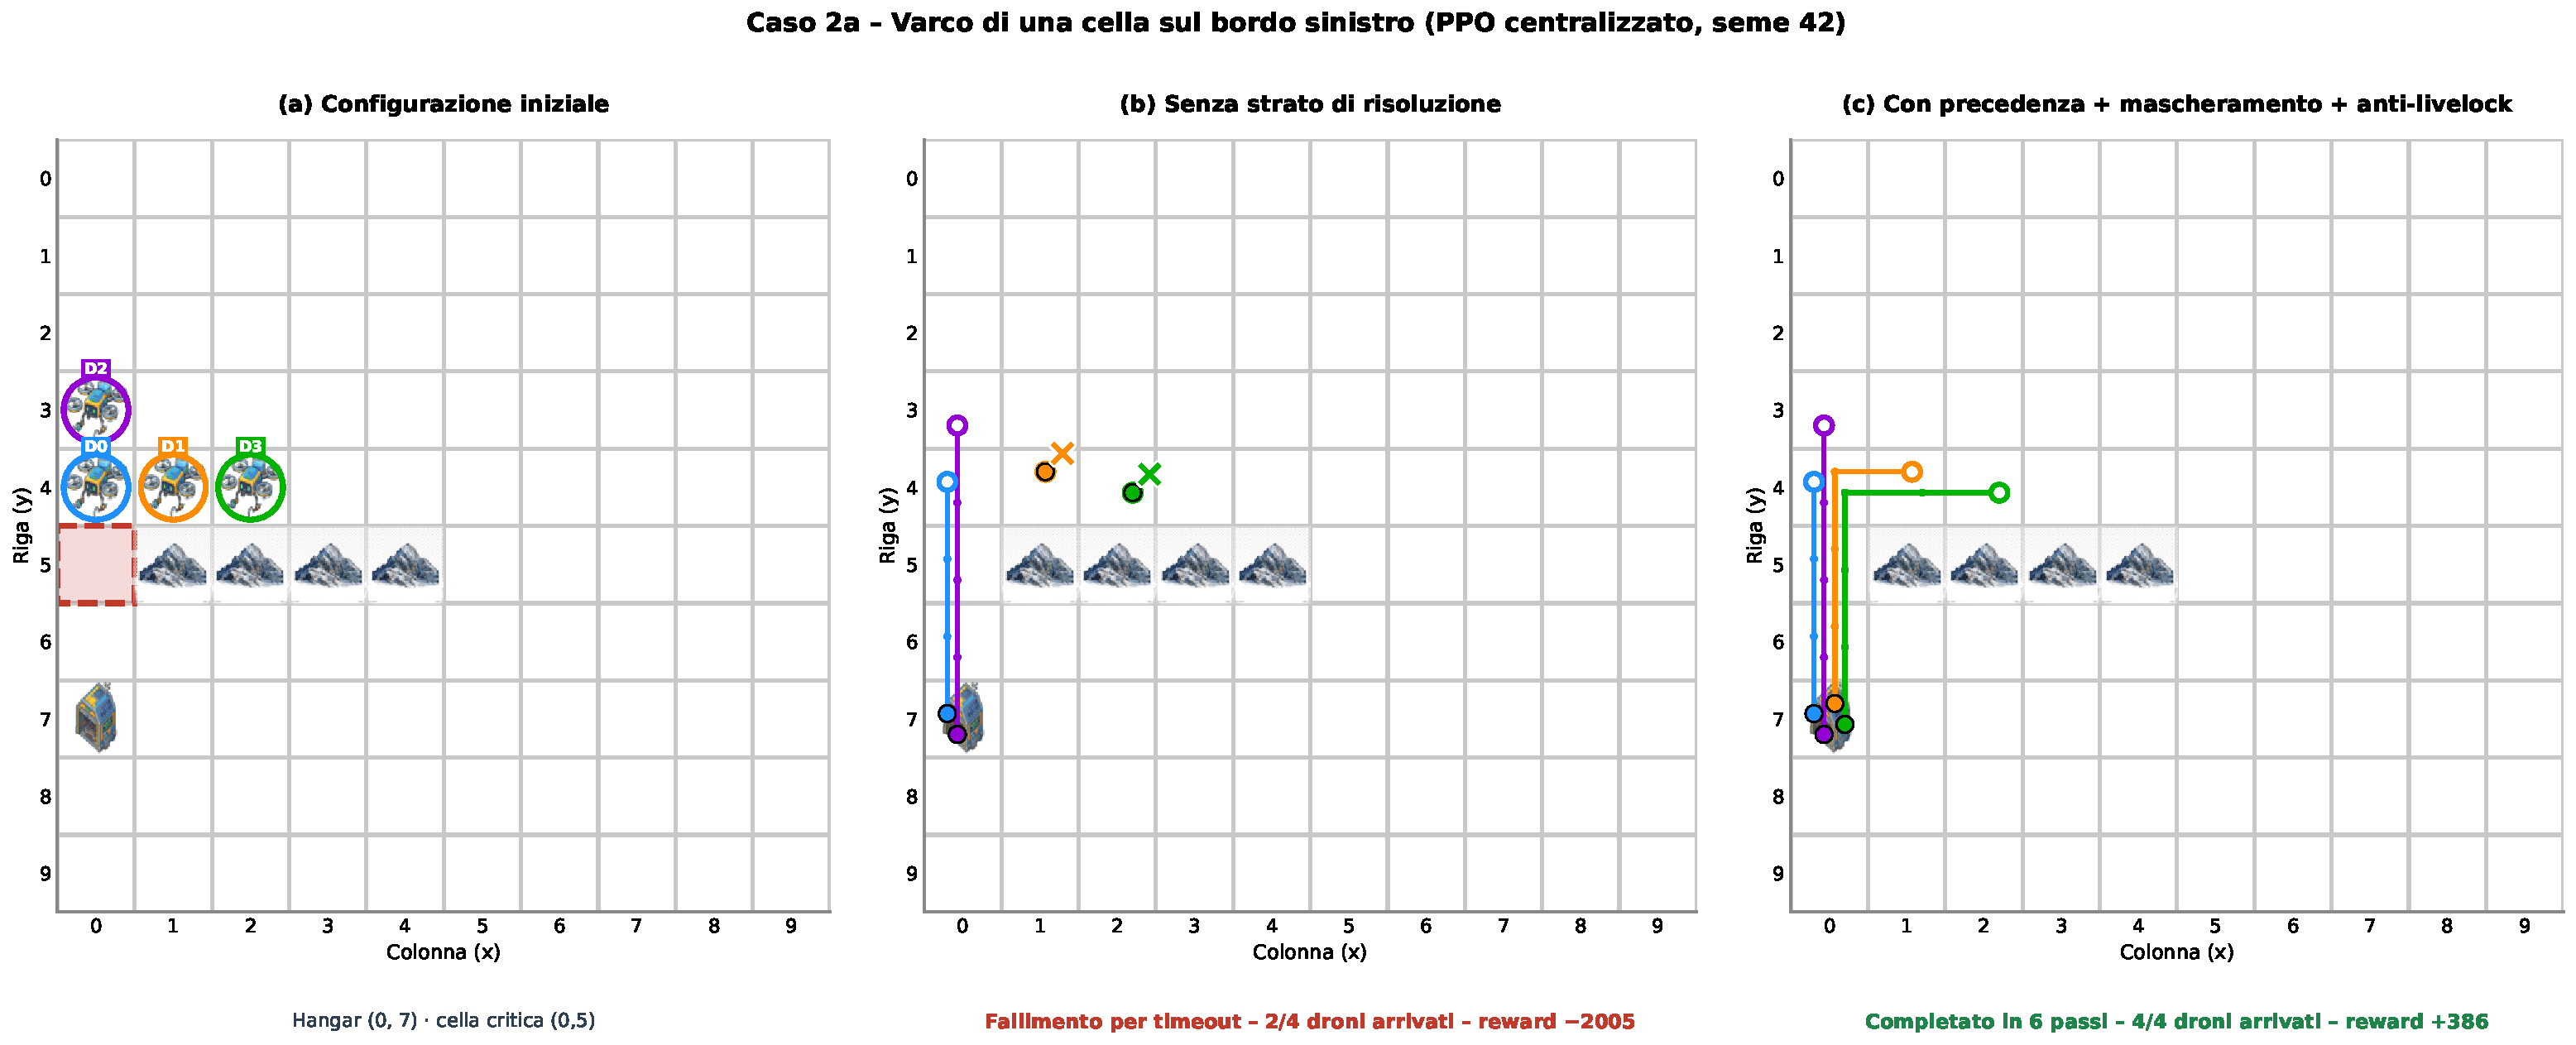
\includegraphics[width=0.95\textwidth]{fig_A_7_caso_2a_ppo.pdf}
    \caption{Caso 2a, PPO (seme 42): configurazione iniziale, traiettorie senza strato e con strato di risoluzione.}
    \label{fig:A_7}
\end{figure}

\noindent\textbf{MAPPO, senza strato di risoluzione.} Fallimento per timeout ($100$ passi) (droni arrivati: 0/4, reward: $-5340$, vertex collision: $98$).

{\footnotesize
\setlength{\tabcolsep}{3.5pt}
\begin{longtable}{c l l >{\raggedright\arraybackslash}p{3.8cm}}
\toprule
\textbf{Passo} & \textbf{Posizioni ($\text{D0} \cdot \text{D1} \cdot \text{D2} \cdot \text{D3}$)} & \textbf{Azioni ($\text{D0} \cdot \text{D1} \cdot \text{D2} \cdot \text{D3}$)} & \textbf{Eventi} \\
\midrule
\endfirsthead
\toprule
\textbf{Passo} & \textbf{Posizioni ($\text{D0} \cdot \text{D1} \cdot \text{D2} \cdot \text{D3}$)} & \textbf{Azioni ($\text{D0} \cdot \text{D1} \cdot \text{D2} \cdot \text{D3}$)} & \textbf{Eventi} \\
\midrule
\endhead
\bottomrule
\endlastfoot
1      & $(0, 4) \cdot (1, 4) \cdot (0, 3) \cdot (2, 4)$ & Giù $\cdot$ Giù $\cdot$ Giù $\cdot$ Giù      & D1$(1, 4)$ urta la montagna in $(1, 5)$; D3$(2, 4)$ urta la montagna in $(2, 5)$ \\
2      & $(0, 5) \cdot (1, 4) \cdot (0, 4) \cdot (2, 4)$ & Giù $\cdot$ Giù $\cdot$ Giù $\cdot$ Giù      & D1$(1, 4)$ urta la montagna in $(1, 5)$; D3$(2, 4)$ urta la montagna in $(2, 5)$ \\
3      & $(0, 6) \cdot (1, 4) \cdot (0, 5) \cdot (2, 4)$ & Sinistra $\cdot$ Giù $\cdot$ Giù $\cdot$ Giù & scontro D0$(0, 6)$ / D2$(0, 5)$ su $(0, 6)$ accanto all'hangar; D1$(1, 4)$ urta la montagna in $(1, 5)$; D3$(2, 4)$ urta la montagna in $(2, 5)$; D0$(0, 6)$ urta il bordo della mappa \\
4--100 & & & D0 resta fermo in $(0, 6)$; D1 resta fermo in $(1, 4)$; D2 resta fermo in $(0, 5)$; D3 resta fermo in $(2, 4)$ \\
\end{longtable}
}

\noindent\textbf{MAPPO, con strato di risoluzione.} Completato con successo in $12$ passi (droni arrivati: 4/4, reward: $+374$, precedenze: $0$, mascheramenti: $9$, anti-livelock: $6$).

{\footnotesize
\setlength{\tabcolsep}{3.5pt}
\begin{longtable}{c l l >{\raggedright\arraybackslash}p{3.8cm}}
\toprule
\textbf{Passo} & \textbf{Posizioni ($\text{D0} \cdot \text{D1} \cdot \text{D2} \cdot \text{D3}$)} & \textbf{Azioni ($\text{D0} \cdot \text{D1} \cdot \text{D2} \cdot \text{D3}$)} & \textbf{Eventi} \\
\midrule
\endfirsthead
\toprule
\textbf{Passo} & \textbf{Posizioni ($\text{D0} \cdot \text{D1} \cdot \text{D2} \cdot \text{D3}$)} & \textbf{Azioni ($\text{D0} \cdot \text{D1} \cdot \text{D2} \cdot \text{D3}$)} & \textbf{Eventi} \\
\midrule
\endhead
\bottomrule
\endlastfoot
1  & $(0, 4) \cdot (1, 4) \cdot (0, 3) \cdot (2, 4)$ & Giù $\cdot$ Destra $\cdot$ Giù $\cdot$ Destra   & mascheramento D1$(1, 4)$: Giù $\to$ Destra; mascheramento D3$(2, 4)$: Giù $\to$ Destra \\
2  & $(0, 5) \cdot (2, 4) \cdot (0, 4) \cdot (3, 4)$ & Giù $\cdot$ Destra $\cdot$ Giù $\cdot$ Destra   & mascheramento D1$(2, 4)$: Giù $\to$ Sinistra; mascheramento D3$(3, 4)$: Giù $\to$ Sinistra; anti-livelock D1$(2, 4)$: Sinistra $\to$ Destra; anti-livelock D3$(3, 4)$: Sinistra $\to$ Destra \\
3  & $(0, 6) \cdot (3, 4) \cdot (0, 5) \cdot (4, 4)$ & Giù $\cdot$ Destra $\cdot$ Giù $\cdot$ Destra   & mascheramento D0$(0, 6)$: Sinistra $\to$ Giù; mascheramento D1$(3, 4)$: Giù $\to$ Sinistra; mascheramento D3$(4, 4)$: Giù $\to$ Sinistra; anti-livelock D1$(3, 4)$: Sinistra $\to$ Destra; anti-livelock D3$(4, 4)$: Sinistra $\to$ Destra \\
4  & $(0, 7) \cdot (4, 4) \cdot (0, 6) \cdot (5, 4)$ & --- $\cdot$ Destra $\cdot$ Giù $\cdot$ Giù      & mascheramento D1$(4, 4)$: Giù $\to$ Sinistra; anti-livelock D1$(4, 4)$: Sinistra $\to$ Destra \\
5  & $(0, 7) \cdot (5, 4) \cdot (0, 7) \cdot (5, 5)$ & --- $\cdot$ Giù $\cdot$ --- $\cdot$ Giù         & anti-livelock D1$(5, 4)$: Sinistra $\to$ Giù \\
6  & $(0, 7) \cdot (5, 5) \cdot (0, 7) \cdot (5, 6)$ & --- $\cdot$ Giù $\cdot$ --- $\cdot$ Sinistra    & mascheramento D1$(5, 5)$: Sinistra $\to$ Giù \\
7  & $(0, 7) \cdot (5, 6) \cdot (0, 7) \cdot (4, 6)$ & --- $\cdot$ Sinistra $\cdot$ --- $\cdot$ Sinistra & si muovono D1, D3 \\
8  & $(0, 7) \cdot (4, 6) \cdot (0, 7) \cdot (3, 6)$ & --- $\cdot$ Sinistra $\cdot$ --- $\cdot$ Sinistra & si muovono D1, D3 \\
9  & $(0, 7) \cdot (3, 6) \cdot (0, 7) \cdot (2, 6)$ & --- $\cdot$ Sinistra $\cdot$ --- $\cdot$ Sinistra & si muovono D1, D3 \\
10 & $(0, 7) \cdot (2, 6) \cdot (0, 7) \cdot (1, 6)$ & --- $\cdot$ Sinistra $\cdot$ --- $\cdot$ Giù    & si muovono D1, D3 \\
11 & $(0, 7) \cdot (1, 6) \cdot (0, 7) \cdot (1, 7)$ & --- $\cdot$ Giù $\cdot$ --- $\cdot$ Sinistra    & si muovono D1, D3 \\
12 & $(0, 7) \cdot (1, 7) \cdot (0, 7) \cdot (0, 7)$ & --- $\cdot$ Sinistra $\cdot$ --- $\cdot$ ---    & si muove D1 \\
\end{longtable}
}

\noindent\textbf{PPO, senza strato di risoluzione.} Fallimento per timeout ($100$ passi) (droni arrivati: 2/4, reward: $-2005$, vertex collision: $0$).

{\footnotesize
\setlength{\tabcolsep}{3.5pt}
\begin{longtable}{c l l >{\raggedright\arraybackslash}p{3.8cm}}
\toprule
\textbf{Passo} & \textbf{Posizioni ($\text{D0} \cdot \text{D1} \cdot \text{D2} \cdot \text{D3}$)} & \textbf{Azioni ($\text{D0} \cdot \text{D1} \cdot \text{D2} \cdot \text{D3}$)} & \textbf{Eventi} \\
\midrule
\endfirsthead
\toprule
\textbf{Passo} & \textbf{Posizioni ($\text{D0} \cdot \text{D1} \cdot \text{D2} \cdot \text{D3}$)} & \textbf{Azioni ($\text{D0} \cdot \text{D1} \cdot \text{D2} \cdot \text{D3}$)} & \textbf{Eventi} \\
\midrule
\endhead
\bottomrule
\endlastfoot
1      & $(0, 4) \cdot (1, 4) \cdot (0, 3) \cdot (2, 4)$ & Giù $\cdot$ Giù $\cdot$ Giù $\cdot$ Giù & D1$(1, 4)$ urta la montagna in $(1, 5)$; D3$(2, 4)$ urta la montagna in $(2, 5)$ \\
2      & $(0, 5) \cdot (1, 4) \cdot (0, 4) \cdot (2, 4)$ & Giù $\cdot$ Giù $\cdot$ Giù $\cdot$ Giù & D1$(1, 4)$ urta la montagna in $(1, 5)$; D3$(2, 4)$ urta la montagna in $(2, 5)$ \\
3      & $(0, 6) \cdot (1, 4) \cdot (0, 5) \cdot (2, 4)$ & Giù $\cdot$ Giù $\cdot$ Giù $\cdot$ Giù & D1$(1, 4)$ urta la montagna in $(1, 5)$; D3$(2, 4)$ urta la montagna in $(2, 5)$ \\
4      & $(0, 7) \cdot (1, 4) \cdot (0, 6) \cdot (2, 4)$ & --- $\cdot$ Giù $\cdot$ Giù $\cdot$ Giù & D1$(1, 4)$ urta la montagna in $(1, 5)$; D3$(2, 4)$ urta la montagna in $(2, 5)$ \\
5      & $(0, 7) \cdot (1, 4) \cdot (0, 7) \cdot (2, 4)$ & --- $\cdot$ Giù $\cdot$ --- $\cdot$ Giù & D1$(1, 4)$ urta la montagna in $(1, 5)$; D3$(2, 4)$ urta la montagna in $(2, 5)$ \\
6--100 & & & D1 resta fermo in $(1, 4)$; D3 resta fermo in $(2, 4)$ \\
\end{longtable}
}

\noindent\textbf{PPO, con strato di risoluzione.} Completato con successo in $6$ passi (droni arrivati: 4/4, reward: $+386$, precedenze: $2$, mascheramenti: $4$, anti-livelock: $0$).

{\footnotesize
\setlength{\tabcolsep}{3.5pt}
\begin{longtable}{c l l >{\raggedright\arraybackslash}p{3.8cm}}
\toprule
\textbf{Passo} & \textbf{Posizioni ($\text{D0} \cdot \text{D1} \cdot \text{D2} \cdot \text{D3}$)} & \textbf{Azioni ($\text{D0} \cdot \text{D1} \cdot \text{D2} \cdot \text{D3}$)} & \textbf{Eventi} \\
\midrule
\endfirsthead
\toprule
\textbf{Passo} & \textbf{Posizioni ($\text{D0} \cdot \text{D1} \cdot \text{D2} \cdot \text{D3}$)} & \textbf{Azioni ($\text{D0} \cdot \text{D1} \cdot \text{D2} \cdot \text{D3}$)} & \textbf{Eventi} \\
\midrule
\endhead
\bottomrule
\endlastfoot
1 & $(0, 4) \cdot (1, 4) \cdot (0, 3) \cdot (2, 4)$ & Giù $\cdot$ Sinistra $\cdot$ Giù $\cdot$ Sinistra & mascheramento D1$(1, 4)$: Giù $\to$ Sinistra; mascheramento D3$(2, 4)$: Giù $\to$ Sinistra; precedenza su $(0, 4)$: passa D1 (distanza $4$), attende D2 (distanza $4$) \\
2 & $(0, 5) \cdot (0, 4) \cdot (0, 3) \cdot (1, 4)$ & Giù $\cdot$ Giù $\cdot$ Giù $\cdot$ Sinistra      & mascheramento D3$(1, 4)$: Giù $\to$ Sinistra; precedenza su $(0, 4)$: passa D2 (distanza $4$), attende D3 (distanza $4$) \\
3 & $(0, 6) \cdot (0, 5) \cdot (0, 4) \cdot (1, 4)$ & Giù $\cdot$ Giù $\cdot$ Giù $\cdot$ Sinistra      & mascheramento D3$(1, 4)$: Giù $\to$ Sinistra \\
4 & $(0, 7) \cdot (0, 6) \cdot (0, 5) \cdot (0, 4)$ & --- $\cdot$ Giù $\cdot$ Giù $\cdot$ Giù           & si muovono D1, D2, D3 \\
5 & $(0, 7) \cdot (0, 7) \cdot (0, 6) \cdot (0, 5)$ & --- $\cdot$ --- $\cdot$ Giù $\cdot$ Giù           & si muovono D2, D3 \\
6 & $(0, 7) \cdot (0, 7) \cdot (0, 7) \cdot (0, 6)$ & --- $\cdot$ --- $\cdot$ --- $\cdot$ Giù           & si muove D3 \\
\end{longtable}
}

% -----------------------------------------------------------------------------
% CASO 2B
% -----------------------------------------------------------------------------
\section{Caso 2b -- Montagne a 1 cella dal bordo superiore}
\label{sec:app_caso_2b}

Montagne in $(5,1)$, $(5,2)$, $(5,3)$, $(5,4)$ che lasciano solo la cella $(5,0)$ libera sul bordo in alto. Hangar in $(7,0)$ e droni in $(4,0)$, $(4,1)$, $(3,0)$, $(4,2)$ che devono passare da $(5,0)$.

\begin{figure}[H]
    \centering
    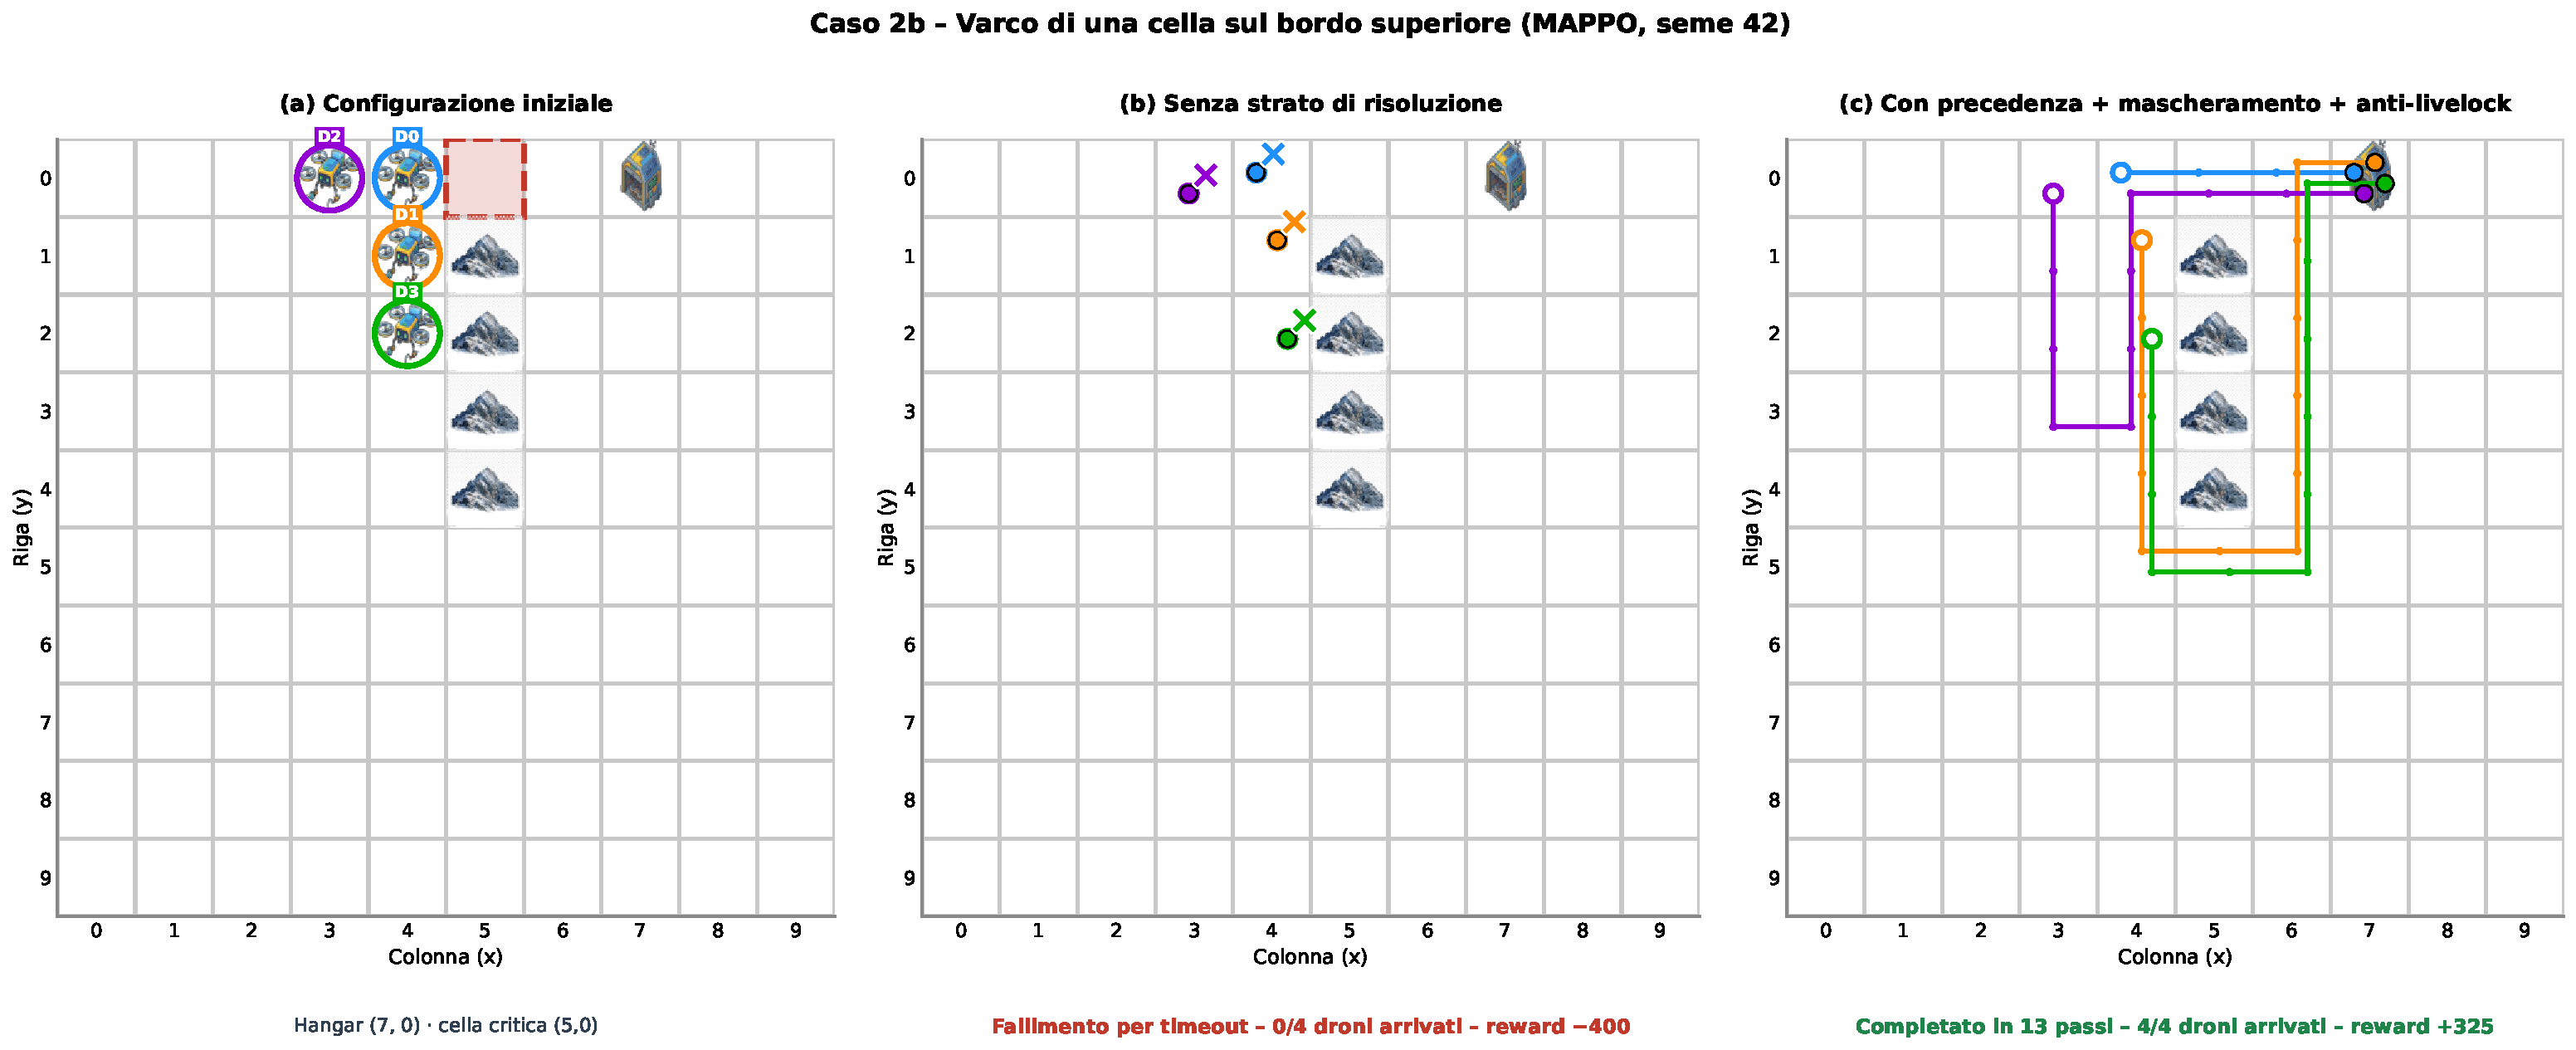
\includegraphics[width=0.95\textwidth]{fig_A_8_caso_2b_mappo.pdf}
    \caption{Caso 2b, MAPPO (seme 42): configurazione iniziale, traiettorie senza strato e con strato di risoluzione.}
    \label{fig:A_8}
\end{figure}

\begin{figure}[H]
    \centering
    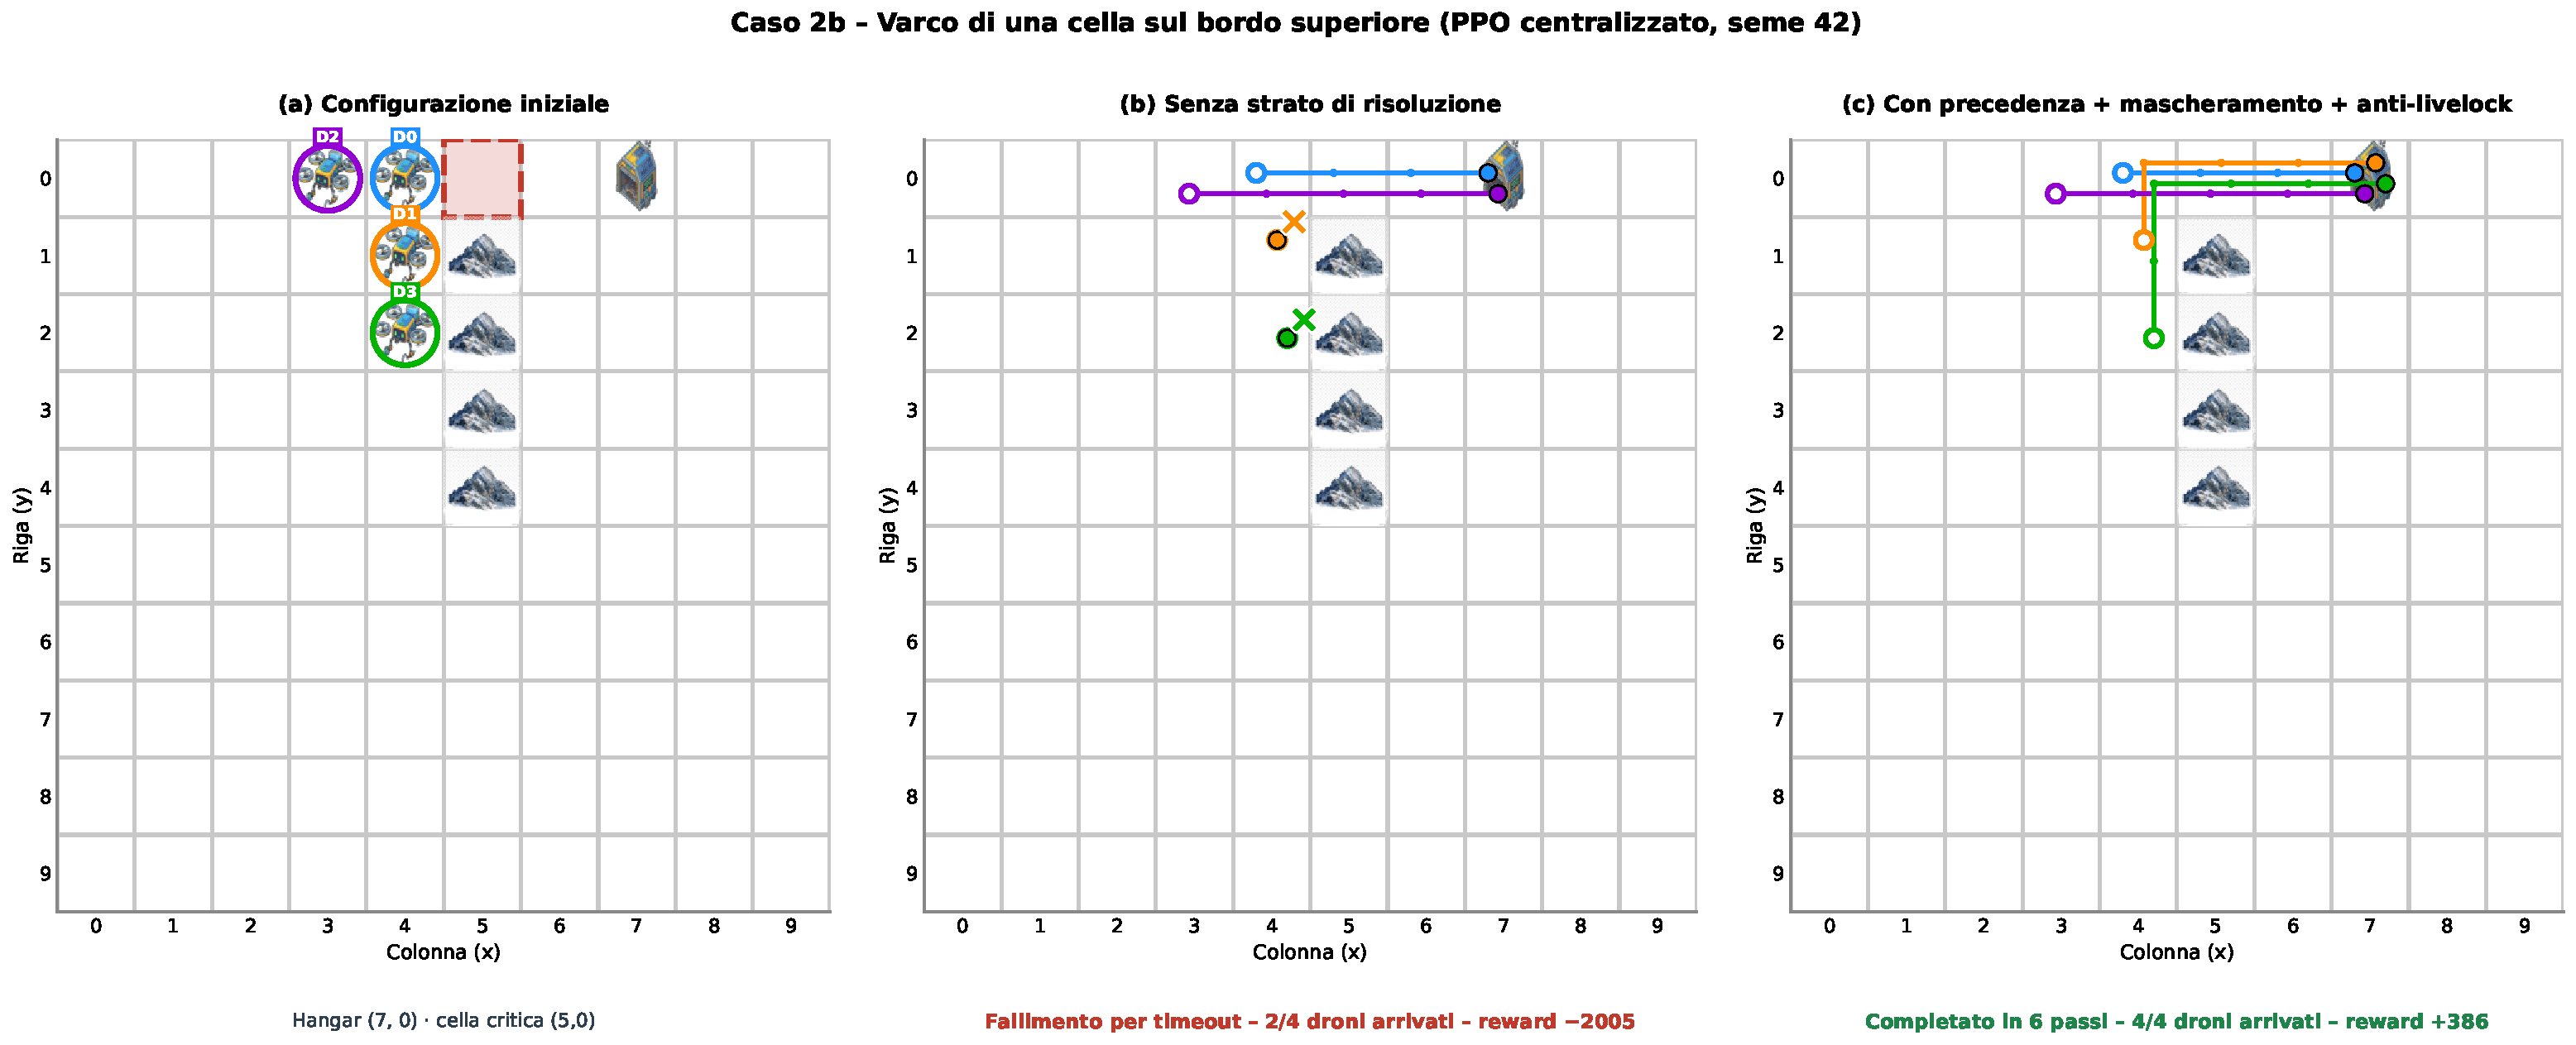
\includegraphics[width=0.95\textwidth]{fig_A_9_caso_2b_ppo.pdf}
    \caption{Caso 2b, PPO (seme 42): configurazione iniziale, traiettorie senza strato e con strato di risoluzione.}
    \label{fig:A_9}
\end{figure}

\noindent\textbf{MAPPO, senza strato di risoluzione.} Fallimento per timeout ($100$ passi) (droni arrivati: 0/4, reward: $-400$, vertex collision: $0$).

{\footnotesize
\setlength{\tabcolsep}{3.5pt}
\begin{longtable}{c l l >{\raggedright\arraybackslash}p{3.8cm}}
\toprule
\textbf{Passo} & \textbf{Posizioni ($\text{D0} \cdot \text{D1} \cdot \text{D2} \cdot \text{D3}$)} & \textbf{Azioni ($\text{D0} \cdot \text{D1} \cdot \text{D2} \cdot \text{D3}$)} & \textbf{Eventi} \\
\midrule
\endfirsthead
\toprule
\textbf{Passo} & \textbf{Posizioni ($\text{D0} \cdot \text{D1} \cdot \text{D2} \cdot \text{D3}$)} & \textbf{Azioni ($\text{D0} \cdot \text{D1} \cdot \text{D2} \cdot \text{D3}$)} & \textbf{Eventi} \\
\midrule
\endhead
\bottomrule
\endlastfoot
1      & $(4, 0) \cdot (4, 1) \cdot (3, 0) \cdot (4, 2)$ & Fermo $\cdot$ Fermo $\cdot$ Fermo $\cdot$ Fermo & restano fermi D0, D1, D2, D3 \\
2--100 & & & D0 resta fermo in $(4, 0)$; D1 resta fermo in $(4, 1)$; D2 resta fermo in $(3, 0)$; D3 resta fermo in $(4, 2)$ \\
\end{longtable}
}

\noindent\textbf{MAPPO, con strato di risoluzione.} Completato con successo in $13$ passi (droni arrivati: 4/4, reward: $+325$, precedenze: $0$, mascheramenti: $39$, anti-livelock: $20$).

{\footnotesize
\setlength{\tabcolsep}{3.5pt}
\begin{longtable}{c l l >{\raggedright\arraybackslash}p{3.8cm}}
\toprule
\textbf{Passo} & \textbf{Posizioni ($\text{D0} \cdot \text{D1} \cdot \text{D2} \cdot \text{D3}$)} & \textbf{Azioni ($\text{D0} \cdot \text{D1} \cdot \text{D2} \cdot \text{D3}$)} & \textbf{Eventi} \\
\midrule
\endfirsthead
\toprule
\textbf{Passo} & \textbf{Posizioni ($\text{D0} \cdot \text{D1} \cdot \text{D2} \cdot \text{D3}$)} & \textbf{Azioni ($\text{D0} \cdot \text{D1} \cdot \text{D2} \cdot \text{D3}$)} & \textbf{Eventi} \\
\midrule
\endhead
\bottomrule
\endlastfoot
1  & $(4, 0) \cdot (4, 1) \cdot (3, 0) \cdot (4, 2)$ & Giù $\cdot$ Giù $\cdot$ Giù $\cdot$ Su       & mascheramento D0$(4, 0)$: Fermo $\to$ Giù; mascheramento D1$(4, 1)$: Fermo $\to$ Giù; mascheramento D2$(3, 0)$: Fermo $\to$ Giù; mascheramento D3$(4, 2)$: Fermo $\to$ Su; scontro D0$(4, 0)$ / D1$(4, 1)$ su $(4, 1)$; scambio bloccato tra D1$(4, 1)$ e D3$(4, 2)$ \\
2  & $(4, 0) \cdot (4, 1) \cdot (3, 1) \cdot (4, 2)$ & Destra $\cdot$ Giù $\cdot$ Giù $\cdot$ Giù   & mascheramento D0$(4, 0)$: Fermo $\to$ Destra; mascheramento D1$(4, 1)$: Fermo $\to$ Giù; mascheramento D2$(3, 1)$: Fermo $\to$ Giù; mascheramento D3$(4, 2)$: Fermo $\to$ Giù \\
3  & $(5, 0) \cdot (4, 2) \cdot (3, 2) \cdot (4, 3)$ & Destra $\cdot$ Giù $\cdot$ Giù $\cdot$ Giù   & mascheramento D0$(5, 0)$: Fermo $\to$ Destra; mascheramento D1$(4, 2)$: Fermo $\to$ Su; mascheramento D2$(3, 2)$: Fermo $\to$ Su; mascheramento D3$(4, 3)$: Fermo $\to$ Su; anti-livelock D1$(4, 2)$: Su $\to$ Giù; anti-livelock D2$(3, 2)$: Su $\to$ Giù; anti-livelock D3$(4, 3)$: Su $\to$ Giù \\
4  & $(6, 0) \cdot (4, 3) \cdot (3, 3) \cdot (4, 4)$ & Destra $\cdot$ Giù $\cdot$ Destra $\cdot$ Giù & mascheramento D0$(6, 0)$: Fermo $\to$ Giù; mascheramento D1$(4, 3)$: Fermo $\to$ Su; mascheramento D2$(3, 3)$: Fermo $\to$ Su; mascheramento D3$(4, 4)$: Fermo $\to$ Su; anti-livelock D0$(6, 0)$: Giù $\to$ Destra; anti-livelock D1$(4, 3)$: Su $\to$ Giù; anti-livelock D2$(3, 3)$: Su $\to$ Destra; anti-livelock D3$(4, 4)$: Su $\to$ Giù \\
5  & $(7, 0) \cdot (4, 4) \cdot (4, 3) \cdot (4, 5)$ & --- $\cdot$ Giù $\cdot$ Su $\cdot$ Destra    & mascheramento D1$(4, 4)$: Fermo $\to$ Su; mascheramento D2$(4, 3)$: Fermo $\to$ Su; mascheramento D3$(4, 5)$: Fermo $\to$ Su; anti-livelock D1$(4, 4)$: Su $\to$ Giù; anti-livelock D3$(4, 5)$: Su $\to$ Destra \\
6  & $(7, 0) \cdot (4, 5) \cdot (4, 2) \cdot (5, 5)$ & --- $\cdot$ Destra $\cdot$ Su $\cdot$ Destra & mascheramento D1$(4, 5)$: Fermo $\to$ Su; mascheramento D2$(4, 2)$: Fermo $\to$ Giù; mascheramento D3$(5, 5)$: Fermo $\to$ Destra; anti-livelock D1$(4, 5)$: Su $\to$ Destra; anti-livelock D2$(4, 2)$: Giù $\to$ Su \\
7  & $(7, 0) \cdot (5, 5) \cdot (4, 1) \cdot (6, 5)$ & --- $\cdot$ Destra $\cdot$ Su $\cdot$ Su     & mascheramento D1$(5, 5)$: Fermo $\to$ Destra; mascheramento D2$(4, 1)$: Fermo $\to$ Giù; mascheramento D3$(6, 5)$: Fermo $\to$ Su; anti-livelock D2$(4, 1)$: Giù $\to$ Su \\
8  & $(7, 0) \cdot (6, 5) \cdot (4, 0) \cdot (6, 4)$ & --- $\cdot$ Su $\cdot$ Destra $\cdot$ Su     & mascheramento D1$(6, 5)$: Fermo $\to$ Su; mascheramento D2$(4, 0)$: Fermo $\to$ Giù; mascheramento D3$(6, 4)$: Fermo $\to$ Su; anti-livelock D2$(4, 0)$: Giù $\to$ Destra \\
9  & $(7, 0) \cdot (6, 4) \cdot (5, 0) \cdot (6, 3)$ & --- $\cdot$ Su $\cdot$ Destra $\cdot$ Su     & mascheramento D1$(6, 4)$: Fermo $\to$ Su; mascheramento D2$(5, 0)$: Fermo $\to$ Destra; mascheramento D3$(6, 3)$: Fermo $\to$ Su \\
10 & $(7, 0) \cdot (6, 3) \cdot (6, 0) \cdot (6, 2)$ & --- $\cdot$ Su $\cdot$ Destra $\cdot$ Su     & mascheramento D1$(6, 3)$: Fermo $\to$ Su; mascheramento D2$(6, 0)$: Fermo $\to$ Giù; mascheramento D3$(6, 2)$: Fermo $\to$ Giù; anti-livelock D2$(6, 0)$: Giù $\to$ Destra; anti-livelock D3$(6, 2)$: Giù $\to$ Su \\
11 & $(7, 0) \cdot (6, 2) \cdot (7, 0) \cdot (6, 1)$ & --- $\cdot$ Su $\cdot$ --- $\cdot$ Su        & mascheramento D1$(6, 2)$: Fermo $\to$ Giù; mascheramento D3$(6, 1)$: Fermo $\to$ Giù; anti-livelock D1$(6, 2)$: Giù $\to$ Su; anti-livelock D3$(6, 1)$: Giù $\to$ Su \\
12 & $(7, 0) \cdot (6, 1) \cdot (7, 0) \cdot (6, 0)$ & --- $\cdot$ Su $\cdot$ --- $\cdot$ Destra    & mascheramento D1$(6, 1)$: Fermo $\to$ Giù; mascheramento D3$(6, 0)$: Fermo $\to$ Giù; anti-livelock D1$(6, 1)$: Giù $\to$ Su; anti-livelock D3$(6, 0)$: Giù $\to$ Destra \\
13 & $(7, 0) \cdot (6, 0) \cdot (7, 0) \cdot (7, 0)$ & --- $\cdot$ Destra $\cdot$ --- $\cdot$ ---   & mascheramento D1$(6, 0)$: Fermo $\to$ Giù; anti-livelock D1$(6, 0)$: Giù $\to$ Destra \\
\end{longtable}
}

\noindent\textbf{PPO, senza strato di risoluzione.} Fallimento per timeout ($100$ passi) (droni arrivati: 2/4, reward: $-2005$, vertex collision: $0$).

{\footnotesize
\setlength{\tabcolsep}{3.5pt}
\begin{longtable}{c l l >{\raggedright\arraybackslash}p{3.8cm}}
\toprule
\textbf{Passo} & \textbf{Posizioni ($\text{D0} \cdot \text{D1} \cdot \text{D2} \cdot \text{D3}$)} & \textbf{Azioni ($\text{D0} \cdot \text{D1} \cdot \text{D2} \cdot \text{D3}$)} & \textbf{Eventi} \\
\midrule
\endfirsthead
\toprule
\textbf{Passo} & \textbf{Posizioni ($\text{D0} \cdot \text{D1} \cdot \text{D2} \cdot \text{D3}$)} & \textbf{Azioni ($\text{D0} \cdot \text{D1} \cdot \text{D2} \cdot \text{D3}$)} & \textbf{Eventi} \\
\midrule
\endhead
\bottomrule
\endlastfoot
1      & $(4, 0) \cdot (4, 1) \cdot (3, 0) \cdot (4, 2)$ & Destra $\cdot$ Destra $\cdot$ Destra $\cdot$ Destra & D1$(4, 1)$ urta la montagna in $(5, 1)$; D3$(4, 2)$ urta la montagna in $(5, 2)$ \\
2      & $(5, 0) \cdot (4, 1) \cdot (4, 0) \cdot (4, 2)$ & Destra $\cdot$ Destra $\cdot$ Destra $\cdot$ Destra & D1$(4, 1)$ urta la montagna in $(5, 1)$; D3$(4, 2)$ urta la montagna in $(5, 2)$ \\
3      & $(6, 0) \cdot (4, 1) \cdot (5, 0) \cdot (4, 2)$ & Destra $\cdot$ Destra $\cdot$ Destra $\cdot$ Destra & D1$(4, 1)$ urta la montagna in $(5, 1)$; D3$(4, 2)$ urta la montagna in $(5, 2)$ \\
4      & $(7, 0) \cdot (4, 1) \cdot (6, 0) \cdot (4, 2)$ & --- $\cdot$ Destra $\cdot$ Destra $\cdot$ Destra    & D1$(4, 1)$ urta la montagna in $(5, 1)$; D3$(4, 2)$ urta la montagna in $(5, 2)$ \\
5      & $(7, 0) \cdot (4, 1) \cdot (7, 0) \cdot (4, 2)$ & --- $\cdot$ Destra $\cdot$ --- $\cdot$ Destra       & D1$(4, 1)$ urta la montagna in $(5, 1)$; D3$(4, 2)$ urta la montagna in $(5, 2)$ \\
6--100 & & & D1 resta fermo in $(4, 1)$; D3 resta fermo in $(4, 2)$ \\
\end{longtable}
}

\noindent\textbf{PPO, con strato di risoluzione.} Completato con successo in $6$ passi (droni arrivati: 4/4, reward: $+386$, precedenze: $2$, mascheramenti: $4$, anti-livelock: $0$).

{\footnotesize
\setlength{\tabcolsep}{3.5pt}
\begin{longtable}{c l l >{\raggedright\arraybackslash}p{3.8cm}}
\toprule
\textbf{Passo} & \textbf{Posizioni ($\text{D0} \cdot \text{D1} \cdot \text{D2} \cdot \text{D3}$)} & \textbf{Azioni ($\text{D0} \cdot \text{D1} \cdot \text{D2} \cdot \text{D3}$)} & \textbf{Eventi} \\
\midrule
\endfirsthead
\toprule
\textbf{Passo} & \textbf{Posizioni ($\text{D0} \cdot \text{D1} \cdot \text{D2} \cdot \text{D3}$)} & \textbf{Azioni ($\text{D0} \cdot \text{D1} \cdot \text{D2} \cdot \text{D3}$)} & \textbf{Eventi} \\
\midrule
\endhead
\bottomrule
\endlastfoot
1 & $(4, 0) \cdot (4, 1) \cdot (3, 0) \cdot (4, 2)$ & Destra $\cdot$ Su $\cdot$ Destra $\cdot$ Su     & mascheramento D1$(4, 1)$: Destra $\to$ Su; mascheramento D3$(4, 2)$: Destra $\to$ Su; precedenza su $(4, 0)$: passa D1 (distanza $4$), attende D2 (distanza $4$) \\
2 & $(5, 0) \cdot (4, 0) \cdot (3, 0) \cdot (4, 1)$ & Destra $\cdot$ Destra $\cdot$ Destra $\cdot$ Su & mascheramento D3$(4, 1)$: Destra $\to$ Su; precedenza su $(4, 0)$: passa D2 (distanza $4$), attende D3 (distanza $4$) \\
3 & $(6, 0) \cdot (5, 0) \cdot (4, 0) \cdot (4, 1)$ & Destra $\cdot$ Destra $\cdot$ Destra $\cdot$ Su & mascheramento D3$(4, 1)$: Destra $\to$ Su \\
4 & $(7, 0) \cdot (6, 0) \cdot (5, 0) \cdot (4, 0)$ & --- $\cdot$ Destra $\cdot$ Destra $\cdot$ Destra & si muovono D1, D2, D3 \\
5 & $(7, 0) \cdot (7, 0) \cdot (6, 0) \cdot (5, 0)$ & --- $\cdot$ --- $\cdot$ Destra $\cdot$ Destra   & si muovono D2, D3 \\
6 & $(7, 0) \cdot (7, 0) \cdot (7, 0) \cdot (6, 0)$ & --- $\cdot$ --- $\cdot$ --- $\cdot$ Destra      & si muove D3 \\
\end{longtable}
}

% -----------------------------------------------------------------------------
% CASO 2C
% -----------------------------------------------------------------------------
\section{Caso 2c -- Passaggio di 1 cella lungo il bordo destro}
\label{sec:app_caso_2c}

Montagne in $(8,5)$, $(8,6)$, $(8,7)$, $(7,7)$ che lasciano un passaggio di $1$ cella sul bordo destro per arrivare all'hangar in $(9,8)$. Droni in partenza da $(9,4)$, $(8,4)$, $(9,3)$, $(7,4)$.

\begin{figure}[H]
    \centering
    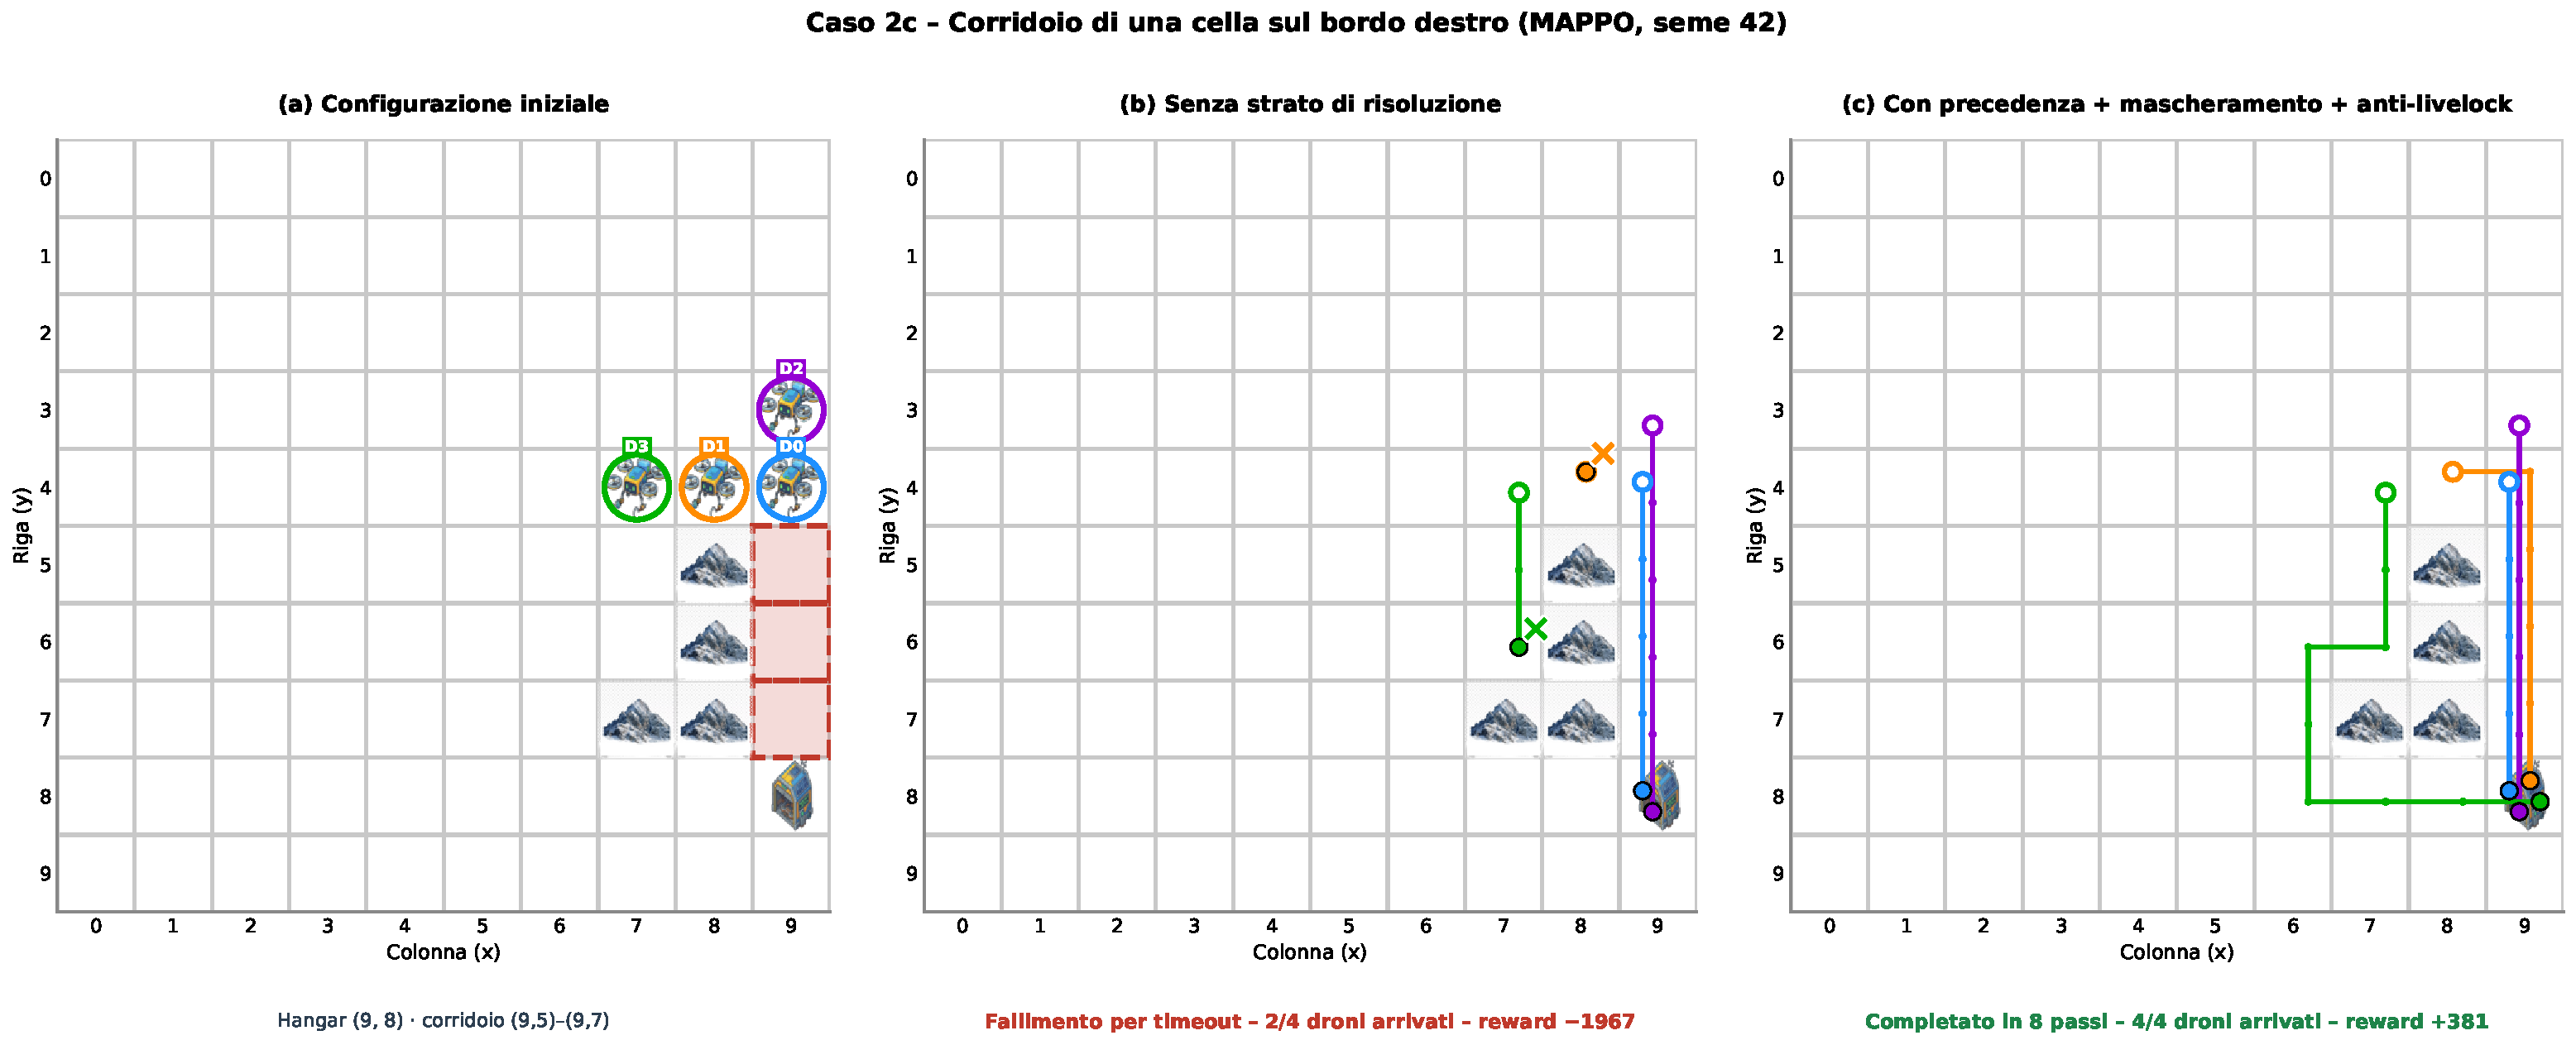
\includegraphics[width=0.95\textwidth]{fig_A_10_caso_2c_mappo.pdf}
    \caption{Caso 2c, MAPPO (seme 42): configurazione iniziale, traiettorie senza strato e con strato di risoluzione.}
    \label{fig:A_10}
\end{figure}

\begin{figure}[H]
    \centering
    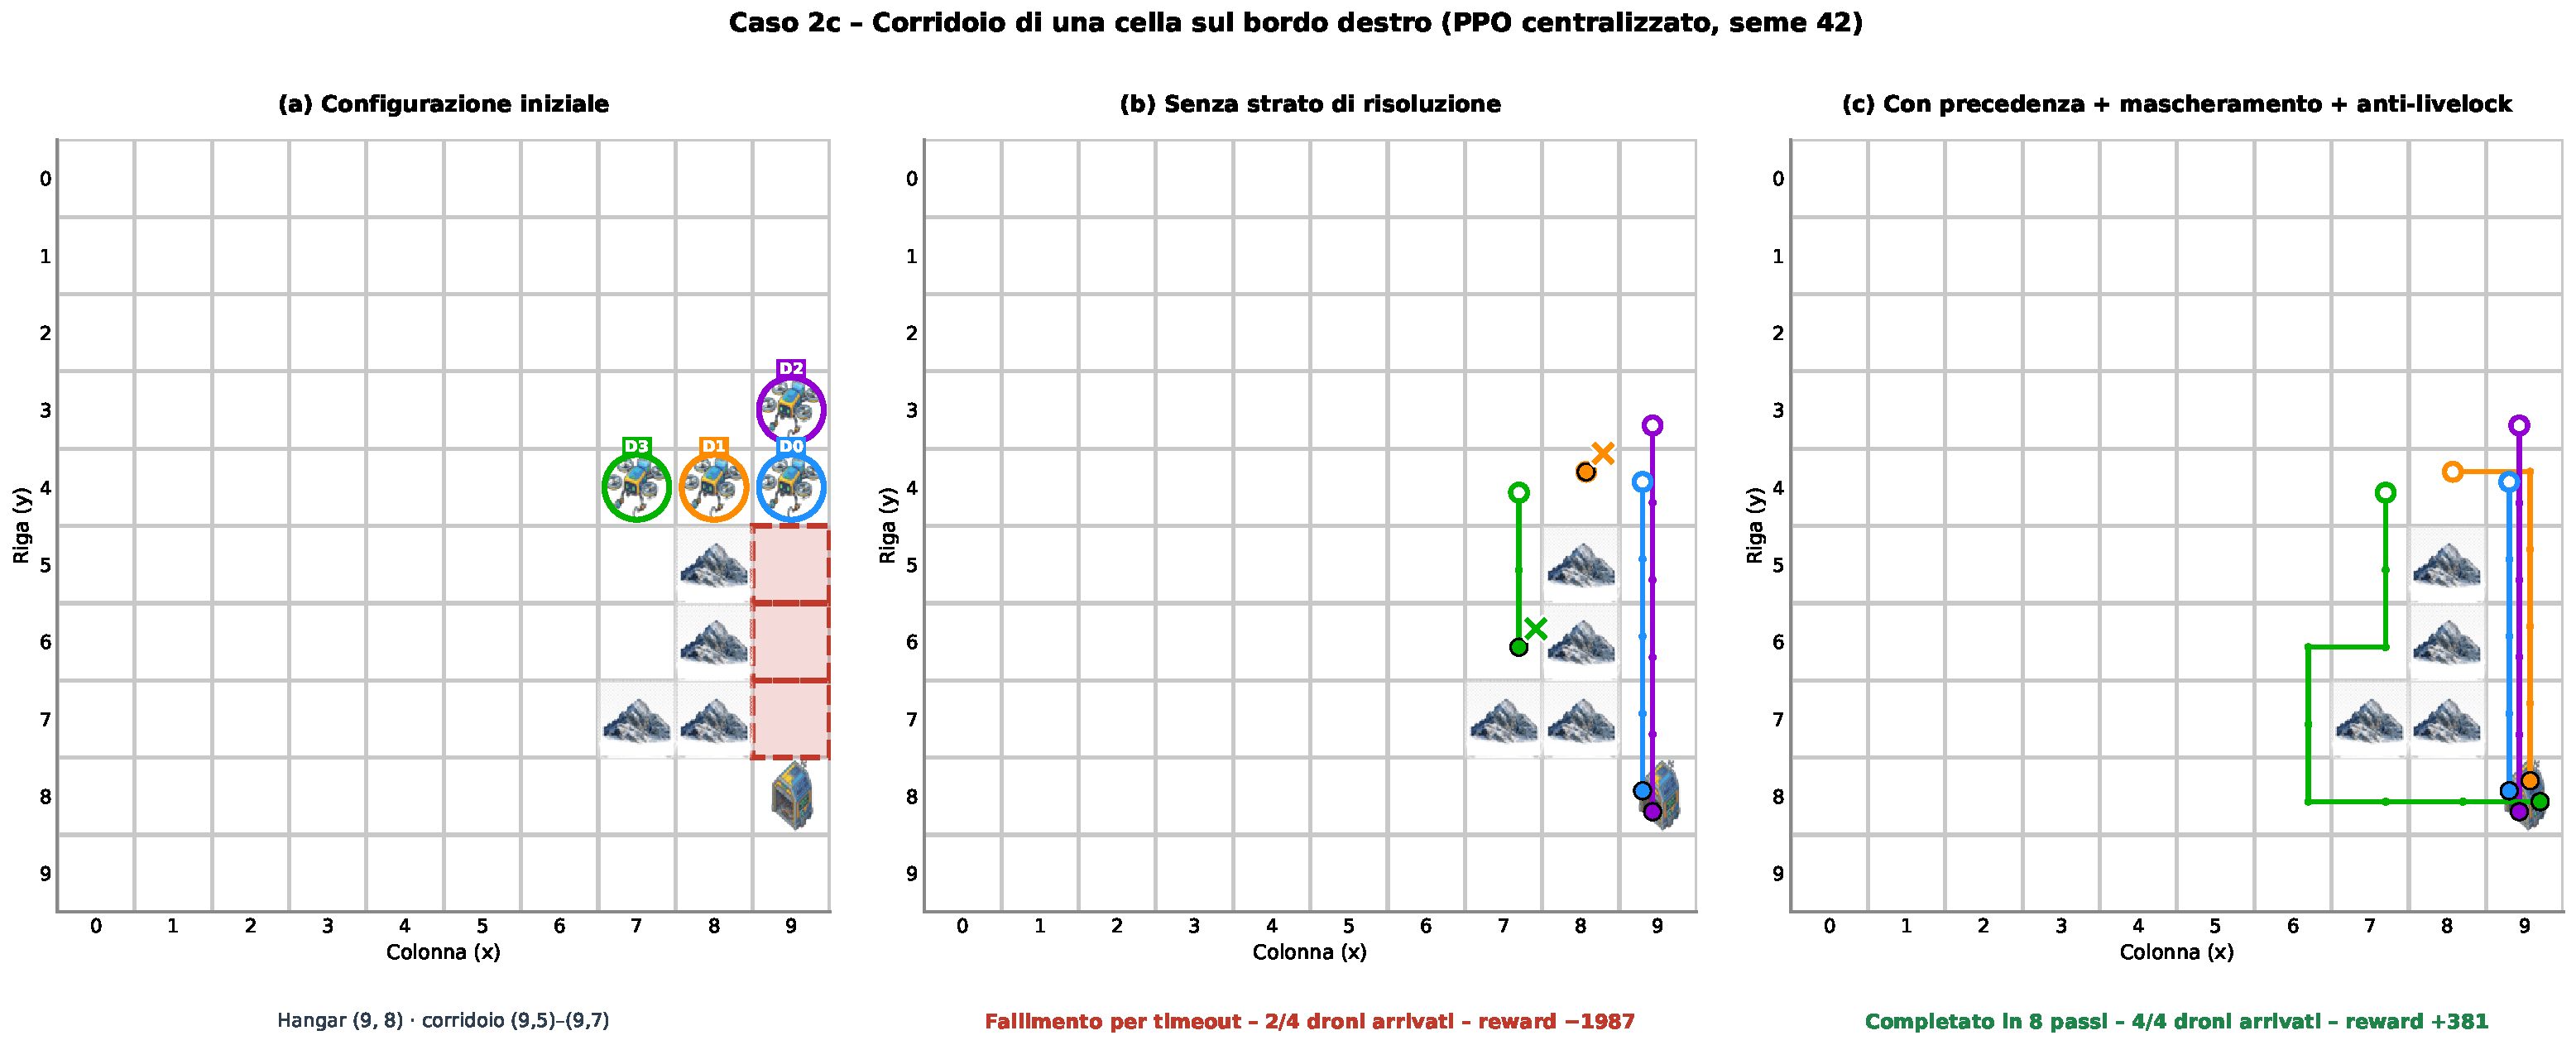
\includegraphics[width=0.95\textwidth]{fig_A_11_caso_2c_ppo.pdf}
    \caption{Caso 2c, PPO (seme 42): configurazione iniziale, traiettorie senza strato e con strato di risoluzione.}
    \label{fig:A_11}
\end{figure}

\noindent\textbf{MAPPO, senza strato di risoluzione.} Fallimento per timeout ($100$ passi) (droni arrivati: 2/4, reward: $-1967$, vertex collision: $0$).

{\footnotesize
\setlength{\tabcolsep}{3.5pt}
\begin{longtable}{c l l >{\raggedright\arraybackslash}p{3.8cm}}
\toprule
\textbf{Passo} & \textbf{Posizioni ($\text{D0} \cdot \text{D1} \cdot \text{D2} \cdot \text{D3}$)} & \textbf{Azioni ($\text{D0} \cdot \text{D1} \cdot \text{D2} \cdot \text{D3}$)} & \textbf{Eventi} \\
\midrule
\endfirsthead
\toprule
\textbf{Passo} & \textbf{Posizioni ($\text{D0} \cdot \text{D1} \cdot \text{D2} \cdot \text{D3}$)} & \textbf{Azioni ($\text{D0} \cdot \text{D1} \cdot \text{D2} \cdot \text{D3}$)} & \textbf{Eventi} \\
\midrule
\endhead
\bottomrule
\endlastfoot
1      & $(9, 4) \cdot (8, 4) \cdot (9, 3) \cdot (7, 4)$ & Giù $\cdot$ Fermo $\cdot$ Giù $\cdot$ Fermo & restano fermi D1, D3 \\
2      & $(9, 5) \cdot (8, 4) \cdot (9, 4) \cdot (7, 4)$ & Giù $\cdot$ Giù $\cdot$ Giù $\cdot$ Giù     & D1$(8, 4)$ urta la montagna in $(8, 5)$ \\
3      & $(9, 6) \cdot (8, 4) \cdot (9, 5) \cdot (7, 5)$ & Giù $\cdot$ Giù $\cdot$ Giù $\cdot$ Giù     & D1$(8, 4)$ urta la montagna in $(8, 5)$ \\
4      & $(9, 7) \cdot (8, 4) \cdot (9, 6) \cdot (7, 6)$ & Giù $\cdot$ Giù $\cdot$ Giù $\cdot$ Giù     & D1$(8, 4)$ urta la montagna in $(8, 5)$; D3$(7, 6)$ urta la montagna in $(7, 7)$ \\
5      & $(9, 8) \cdot (8, 4) \cdot (9, 7) \cdot (7, 6)$ & --- $\cdot$ Giù $\cdot$ Giù $\cdot$ Giù     & D1$(8, 4)$ urta la montagna in $(8, 5)$; D3$(7, 6)$ urta la montagna in $(7, 7)$ \\
6      & $(9, 8) \cdot (8, 4) \cdot (9, 8) \cdot (7, 6)$ & --- $\cdot$ Giù $\cdot$ --- $\cdot$ Giù     & D1$(8, 4)$ urta la montagna in $(8, 5)$; D3$(7, 6)$ urta la montagna in $(7, 7)$ \\
7--100 & & & D1 resta fermo in $(8, 4)$; D3 resta fermo in $(7, 6)$ \\
\end{longtable}
}

\noindent\textbf{MAPPO, con strato di risoluzione.} Completato con successo in $8$ passi (droni arrivati: 4/4, reward: $+381$, precedenze: $1$, mascheramenti: $6$, anti-livelock: $2$).

{\footnotesize
\setlength{\tabcolsep}{3.5pt}
\begin{longtable}{c l l >{\raggedright\arraybackslash}p{3.8cm}}
\toprule
\textbf{Passo} & \textbf{Posizioni ($\text{D0} \cdot \text{D1} \cdot \text{D2} \cdot \text{D3}$)} & \textbf{Azioni ($\text{D0} \cdot \text{D1} \cdot \text{D2} \cdot \text{D3}$)} & \textbf{Eventi} \\
\midrule
\endfirsthead
\toprule
\textbf{Passo} & \textbf{Posizioni ($\text{D0} \cdot \text{D1} \cdot \text{D2} \cdot \text{D3}$)} & \textbf{Azioni ($\text{D0} \cdot \text{D1} \cdot \text{D2} \cdot \text{D3}$)} & \textbf{Eventi} \\
\midrule
\endhead
\bottomrule
\endlastfoot
1 & $(9, 4) \cdot (8, 4) \cdot (9, 3) \cdot (7, 4)$ & Giù $\cdot$ Destra $\cdot$ Giù $\cdot$ Giù   & mascheramento D1$(8, 4)$: Fermo $\to$ Destra; mascheramento D3$(7, 4)$: Fermo $\to$ Giù; precedenza su $(9, 4)$: passa D1 (distanza $5$), attende D2 (distanza $5$) \\
2 & $(9, 5) \cdot (9, 4) \cdot (9, 3) \cdot (7, 5)$ & Giù $\cdot$ Giù $\cdot$ Giù $\cdot$ Giù      & mascheramento D3$(7, 5)$: Fermo $\to$ Giù \\
3 & $(9, 6) \cdot (9, 5) \cdot (9, 4) \cdot (7, 6)$ & Giù $\cdot$ Giù $\cdot$ Giù $\cdot$ Sinistra & mascheramento D3$(7, 6)$: Giù $\to$ Su; anti-livelock D3$(7, 6)$: Su $\to$ Sinistra \\
4 & $(9, 7) \cdot (9, 6) \cdot (9, 5) \cdot (6, 6)$ & Giù $\cdot$ Giù $\cdot$ Giù $\cdot$ Giù      & si muovono D0, D1, D2, D3 \\
5 & $(9, 8) \cdot (9, 7) \cdot (9, 6) \cdot (6, 7)$ & --- $\cdot$ Giù $\cdot$ Giù $\cdot$ Giù      & mascheramento D3$(6, 7)$: Fermo $\to$ Giù \\
6 & $(9, 8) \cdot (9, 8) \cdot (9, 7) \cdot (6, 8)$ & --- $\cdot$ --- $\cdot$ Giù $\cdot$ Destra   & si muovono D2, D3 \\
7 & $(9, 8) \cdot (9, 8) \cdot (9, 8) \cdot (7, 8)$ & --- $\cdot$ --- $\cdot$ --- $\cdot$ Destra   & si muove D3 \\
8 & $(9, 8) \cdot (9, 8) \cdot (9, 8) \cdot (8, 8)$ & --- $\cdot$ --- $\cdot$ --- $\cdot$ Destra   & mascheramento D3$(8, 8)$: Fermo $\to$ Giù; anti-livelock D3$(8, 8)$: Giù $\to$ Destra \\
\end{longtable}
}

\noindent\textbf{PPO, senza strato di risoluzione.} Fallimento per timeout ($100$ passi) (droni arrivati: 2/4, reward: $-1987$, vertex collision: $0$).

{\footnotesize
\setlength{\tabcolsep}{3.5pt}
\begin{longtable}{c l l >{\raggedright\arraybackslash}p{3.8cm}}
\toprule
\textbf{Passo} & \textbf{Posizioni ($\text{D0} \cdot \text{D1} \cdot \text{D2} \cdot \text{D3}$)} & \textbf{Azioni ($\text{D0} \cdot \text{D1} \cdot \text{D2} \cdot \text{D3}$)} & \textbf{Eventi} \\
\midrule
\endfirsthead
\toprule
\textbf{Passo} & \textbf{Posizioni ($\text{D0} \cdot \text{D1} \cdot \text{D2} \cdot \text{D3}$)} & \textbf{Azioni ($\text{D0} \cdot \text{D1} \cdot \text{D2} \cdot \text{D3}$)} & \textbf{Eventi} \\
\midrule
\endhead
\bottomrule
\endlastfoot
1      & $(9, 4) \cdot (8, 4) \cdot (9, 3) \cdot (7, 4)$ & Giù $\cdot$ Giù $\cdot$ Giù $\cdot$ Giù & D1$(8, 4)$ urta la montagna in $(8, 5)$ \\
2      & $(9, 5) \cdot (8, 4) \cdot (9, 4) \cdot (7, 5)$ & Giù $\cdot$ Giù $\cdot$ Giù $\cdot$ Giù & D1$(8, 4)$ urta la montagna in $(8, 5)$ \\
3      & $(9, 6) \cdot (8, 4) \cdot (9, 5) \cdot (7, 6)$ & Giù $\cdot$ Giù $\cdot$ Giù $\cdot$ Giù & D1$(8, 4)$ urta la montagna in $(8, 5)$; D3$(7, 6)$ urta la montagna in $(7, 7)$ \\
4      & $(9, 7) \cdot (8, 4) \cdot (9, 6) \cdot (7, 6)$ & Giù $\cdot$ Giù $\cdot$ Giù $\cdot$ Giù & D1$(8, 4)$ urta la montagna in $(8, 5)$; D3$(7, 6)$ urta la montagna in $(7, 7)$ \\
5      & $(9, 8) \cdot (8, 4) \cdot (9, 7) \cdot (7, 6)$ & --- $\cdot$ Giù $\cdot$ Giù $\cdot$ Giù & D1$(8, 4)$ urta la montagna in $(8, 5)$; D3$(7, 6)$ urta la montagna in $(7, 7)$ \\
6      & $(9, 8) \cdot (8, 4) \cdot (9, 8) \cdot (7, 6)$ & --- $\cdot$ Giù $\cdot$ --- $\cdot$ Giù & D1$(8, 4)$ urta la montagna in $(8, 5)$; D3$(7, 6)$ urta la montagna in $(7, 7)$ \\
7--100 & & & D1 resta fermo in $(8, 4)$; D3 resta fermo in $(7, 6)$ \\
\end{longtable}
}

\noindent\textbf{PPO, con strato di risoluzione.} Completato con successo in $8$ passi (droni arrivati: 4/4, reward: $+381$, precedenze: $1$, mascheramenti: $3$, anti-livelock: $0$).

{\footnotesize
\setlength{\tabcolsep}{3.5pt}
\begin{longtable}{c l l >{\raggedright\arraybackslash}p{3.8cm}}
\toprule
\textbf{Passo} & \textbf{Posizioni ($\text{D0} \cdot \text{D1} \cdot \text{D2} \cdot \text{D3}$)} & \textbf{Azioni ($\text{D0} \cdot \text{D1} \cdot \text{D2} \cdot \text{D3}$)} & \textbf{Eventi} \\
\midrule
\endfirsthead
\toprule
\textbf{Passo} & \textbf{Posizioni ($\text{D0} \cdot \text{D1} \cdot \text{D2} \cdot \text{D3}$)} & \textbf{Azioni ($\text{D0} \cdot \text{D1} \cdot \text{D2} \cdot \text{D3}$)} & \textbf{Eventi} \\
\midrule
\endhead
\bottomrule
\endlastfoot
1 & $(9, 4) \cdot (8, 4) \cdot (9, 3) \cdot (7, 4)$ & Giù $\cdot$ Destra $\cdot$ Giù $\cdot$ Giù   & mascheramento D1$(8, 4)$: Giù $\to$ Destra; precedenza su $(9, 4)$: passa D1 (distanza $5$), attende D2 (distanza $5$) \\
2 & $(9, 5) \cdot (9, 4) \cdot (9, 3) \cdot (7, 5)$ & Giù $\cdot$ Giù $\cdot$ Giù $\cdot$ Giù      & si muovono D0, D1, D2, D3 \\
3 & $(9, 6) \cdot (9, 5) \cdot (9, 4) \cdot (7, 6)$ & Giù $\cdot$ Giù $\cdot$ Giù $\cdot$ Sinistra & mascheramento D3$(7, 6)$: Giù $\to$ Sinistra \\
4 & $(9, 7) \cdot (9, 6) \cdot (9, 5) \cdot (6, 6)$ & Giù $\cdot$ Giù $\cdot$ Giù $\cdot$ Giù      & si muovono D0, D1, D2, D3 \\
5 & $(9, 8) \cdot (9, 7) \cdot (9, 6) \cdot (6, 7)$ & --- $\cdot$ Giù $\cdot$ Giù $\cdot$ Giù      & mascheramento D3$(6, 7)$: Destra $\to$ Giù \\
6 & $(9, 8) \cdot (9, 8) \cdot (9, 7) \cdot (6, 8)$ & --- $\cdot$ --- $\cdot$ Giù $\cdot$ Destra   & si muovono D2, D3 \\
7 & $(9, 8) \cdot (9, 8) \cdot (9, 8) \cdot (7, 8)$ & --- $\cdot$ --- $\cdot$ --- $\cdot$ Destra   & si muove D3 \\
8 & $(9, 8) \cdot (9, 8) \cdot (9, 8) \cdot (8, 8)$ & --- $\cdot$ --- $\cdot$ --- $\cdot$ Destra   & si muove D3 \\
\end{longtable}
}

% =============================================================================
% BIBLIOGRAFIA
% =============================================================================
\cleardoublepage
\phantomsection
\addcontentsline{toc}{chapter}{\bibname}
\nocite{*}
\bibliographystyle{plainnat}
\bibliography{bibliografia}

\end{document}
